\documentclass[11pt,openany]{amsbook}
\renewcommand\citeform[1]{{#1}}
\usepackage{capt-of}
\usepackage{xcolor}
\usepackage{comment}
\usepackage{amsmath}
\usepackage{multicol}
\usepackage{stmaryrd}
\usepackage[margin=1.25in]{geometry}
\usepackage{pifont}
\usepackage{amsfonts}
\usepackage{mathtools}
\usepackage{array}
\usepackage{tabularx}
\usepackage{setspace}
\usepackage{dsfont}
\usepackage{amssymb}
\usepackage{amsthm}
\usepackage{graphicx}
\usepackage{microtype}
\usepackage{tikz-cd}
\usepackage{quiver}
\usepackage{enumitem}
\usepackage{nicefrac}
\usepackage{scalerel}[2016/12/29]
\usepackage{etoolbox}
\usepackage{setspace}
\pagestyle{plain}
\makeatletter
\patchcmd\@thm
  {\let\thm@indent\indent}{\let\thm@indent\noindent}%
  {}{}
\makeatother
\usepackage{etoolbox}

\expandafter\patchcmd\csname\string\proof\endcsname
  {\normalparindent}{0pt }{}{}
\setstretch{1.1}
\usepackage{hyperref}
\usepackage[capitalise]{cleveref}
\usepackage{mathrsfs}
\usepackage[english]{babel}
\usepackage[mathscr]{euscript}
\usepackage{mlmodern}
\usepackage[T1]{fontenc}
\usepackage[]{mdframed}

\newtheoremstyle{propositions} % name
    {1em plus .2em minus .1em}                    % Space above
    {1em plus .2em minus .1em}                    % Space below
    {\itshape}                   % Body font
    {}                           % Indent amount
    {\bfseries}                   % Theorem head font
    {.}                          % Punctuation after theorem head
    {.5em}                       % Space after theorem head
    {}  % Theorem head spec (can be left empty, meaning ‘normal’)

    \theoremstyle{propositions}
\newtheorem{thm}{Theorem}[section]
 \newtheorem{lem}[thm]{Lemma}
\newtheorem{prop}[thm]{Proposition}
\newtheorem{rec}[thm]{Recollection}
\newtheorem*{prop*}{Proposition}
\crefname{prop}{Proposition}{Propositions}
\newtheorem{cor}[thm]{Corollary}
\crefname{cor}{Corollary}{Corollaries}
\theoremstyle{definition}
\newtheorem{const}[thm]{Construction}
\newtheorem{defn}[thm]{Definition}
\newtheorem{notn}[thm]{Notation}
\crefname{const}{Construction}{Constructions}
\crefname{defn}{Definition}{Definitions}
\newtheorem{ex}[thm]{Example}
\newtheorem{recdef}[thm]{Recollection}
\crefname{thm}{Theorem}{Theorems}
\newtheorem{conv}[thm]{Convention}
\theoremstyle{remark}
\newtheorem{rem}[thm]{Remark}
\crefname{rem}{Remark}{Remarks}
\newtheorem*{sk}{Sketch}
%Alternative command to the abstracts of chapters. Thanks to egreg



\newcommand\tcof{\stackrel{\scriptstyle\sim}{\smash{\hookrightarrow}\rule{0pt}{0.4ex}}}



\newcommand{\rightarrowdbl}{\rightarrow\mathrel{\mkern-14mu}\rightarrow}

\newcommand{\xrightarrowdbl}[2][]{%
  \xrightarrow[#1]{#2}\mathrel{\mkern-14mu}\rightarrow
}
\newcommand{\wkeq}{\xrightarrow{
   \,\smash{\raisebox{-0.65ex}{\ensuremath{\scriptstyle\sim}}}\,}}
\newcommand\genmathchar[6]{%
    \newcommand*#1{#3{%
        \mathchoice
            {\hbox{#4\char#2}}%
            {\hbox{#4\char#2}}%
            {\hbox{#5\char#2}}%
            {\hbox{#6\char#2}}%
    }}%
}


\newcommand{\tfib}{\xrightarrowdbl{
   \,\smash{\raisebox{-0.65ex}{\ensuremath{\scriptstyle\sim}}}\,}}
\newcommand\gennnmathchar[6]{%
    \newcommand*#1{#3{%
        \mathchoice
            {\hbox{#4\char#2}}%
            {\hbox{#4\char#2}}%
            {\hbox{#5\char#2}}%
            {\hbox{#6\char#2}}%
    }}%
}
\newcommand{\boxstar}{\mathbin{\mathrlap{\star}{\scaleobj{0.69}{\square}}}}


\makeatletter
\def\subsection{\@startsection{subsection}{2}%
    \z@{.5\linespacing\@plus.7\linespacing}{-.5em}%
    {\normalfont\bfseries}}
\makeatother








\begin{document}

\newgeometry{margin=5cm}
\pagenumbering{gobble}
\hrule
\vspace{0.5cm}
\begin{center}
	{\LARGE \textsc{Examples of $\infty $-Categories}}
\end{center}
\vspace{0.5cm}
\hrule
\vspace{2cm}
\begin{center}
{\Large Balaji Subramoniam \\
	\vspace{0.5cm}
(Chennai Mathematical Institute)}
\end{center}
\vspace{2cm}
\begin{center}
 {\Large Supervisor: Prof. Neil Strickland \\
	\vspace{0.5cm}
Internal Supervisor: Prof. Sukhendu Mehrotra}

\end{center}
\vspace{2cm}
\begin{center}
	{\Large A dissertation submitted for the degree of \\ Master of Science (Mathematics) \\ \vspace{1cm} July 2024}
\end{center}

\newpage
\begin{center}
	{\Large \textbf{Abstract}}
\end{center}
\vspace{1cm}
In this dissertation, we aim to study locally $k$-truncated $\infty $-categories (that is, $\infty $-categories whose mapping spaces are $k$-truncated Kan complexes) for $k=-1,0$ and compare their homotopy theories to those of preorders and categories respectively. In the build up to this, we review some elementary ideas in the theory of $\infty $-categories, model categories and $(\infty ,2)$-categories. We also survey the work of Gagna, Harpaz and Lanari (\cite{GHL}) establishing an equivalence of different descriptions of fibrant objects in the model structure for $(\infty ,2)$-categories. 
\restoregeometry

\newpage
\begin{center}
	{\Large \textbf{Acknowledgements}}
\end{center}
\vspace{1.5cm}
\par This dissertation would not have been possible without the guidance, encouragement and support of many people, academically and otherwise. First and foremost, I am greatly indebted to my advisor, Prof. Neil Strickland, who has been very kind to take time out of his busy schedule to guide me on this project, which turned out to be an immense learning experience for me. Throughout this year-long endeavour, I have significantly benefitted from his invaluable guidance, detailed comments and suggestions on my work, and patience and support through stretches of time when I could make very little progress. I thank my internal advisor Prof. Sukhendu Mehrotra for helpful advice on a variety of things and for his unwavering support throughout. It was under his supervision that I first started working on topics close to this dissertation. I am deeply grateful to my faculty advisors, especially Prof. Upendra Kulkarni, for their patience, understanding and support through thick and thin. I am also immensely grateful to Prof. Pranav Pandit for accepting to review the dissertation and for providing suggestions for improvement in a very short time-frame. I thank Lakshay, my most beloved senior, for getting me interested in category theory and algebraic topology, over countless interesting discussions. I am grateful to Advait for his assistance in proof-reading parts of the dissertation and for carefully verifying some of the proofs that appear here in their raw (and at times painfully constructive) forms. I thank Ankit for keeping me entertained with plenty of mathematical conversations on a variety of topics. I am thankful to Prasanna for introducing me to the idea of using Vim to typeset maths efficiently.

 I am deeply grateful to Chennai Mathematical Institute for this opportunity and to all its members for creating an environment conducive to academic work.  I am glad to have been part of a close-knit group of seven batchmates -- Advait, Aniruddha, Atharva, Bhavesh, Sumantha and Ujjwal -- who made it a memorable couple of years. I thank Aniruddha, Paarth, Shahnaz, Soham and Vedant for their assistance with certain non-academic matters relevant to the dissertation. I am particularly grateful to Aniruddha, for keeping company during the late nights I spent working on this dissertation and for being the best roommate and friend. Lastly and most importantly, I thank my parents for their continuous support and encouragement.

\newpage
\begin{center}
	{\Large \textbf{Introduction}}
\end{center}
\vspace{1cm}
\subsection*{Main Goals} 
In 1973, Boardman and Vogt introduced $\infty$-categories (also called quasicategories or weak Kan complexes) in their study of homotopy coherent algebraic structures (see \cite[Definition 4.8]{BV}).  These were later studied carefully, especially by Joyal and Lurie, and developed into an efficient framework to deal with homotopy coherent mathematics. In simple terms, $\infty $-categories (see \cref{defn:infcat}) are simplicial sets (see \cref{defn:sset}) satisfying certain extension conditions and constitute a model of higher categories with $n$-morphisms for each $n>0$ such that all higher morphisms (that is, $n$-morphisms for $n>1$) are invertible. 

Desirably, one can study categories and topological spaces within the framework of $\infty $-categories and many constructions in category theory and algebraic topology admit appropriate analogues in the setting of $\infty $-categories. To begin with, we have the (classical) nerve construction (see \cref{defn:nerveho}), a fully faithful functor that associates to each category an $\infty $-category. In particular, passing from a category to its nerve leads to no loss in information and hence, we shall not distinguish between categories and their nerves. On the other hand, the singular complex functor (see \cref{singcomp}) associates to each topological space an $\infty $-category that retains information on the topological space up to weak homotopy equivalence.  
A larger subcollection of $\infty $-categories containing all the singular complexes, namely that of Kan complexes (\cref{defn:infcat}), are of special interest. Kan complexes are suitably interpreted as a substitute for topological spaces (up to homotopy type) in the setting of $\infty $-categories (see \S \hyperref[2.2.1]{2.2.1} and (5)-(7), \cref{rem:kanrightproper}). Owing to this, we use the terms `spaces' and `Kan complexes' more or less interchangeably and for the most part, our choice is dictated by the interpretation we prefer to stress on.

Closely related to this is the story of `Grothendieck's homotopy hypothesis'. In a letter to Quillen in 1983 (see \cite{PS}), Grothendieck discusses a generalisation of the Poincar\'{e} fundamental groupoid, namely the ``fundamental $n$-groupoid'' $\prod_n X$  of a topological space $X$, which he expects to capture the $n$-homotopy type of $X$. The rough underlying idea is that the objects of the fundamental $n$-groupoid should be the points in $X$, $1$-morphisms should be homotopy classes of paths between points, $2$-morphisms should be homotopies between $1$-morphisms etc. Inspired by the work of Brown et al., he conjectures the existence of a more general and satisfactory theory of $n$-groupoids (resp. $\infty $-groupoids) that coincides with the theory of $n$-truncated homotopy types (resp. homotopy types) of topological spaces and proposes precise definitions based on ``globular categories'' (see \cite{Malt} for more details). Meanwhile, in a letter to Grothendieck, Porter suggests the use of Kan complexes to model $\infty $-groupoids as envisioned by Grothendieck.

Just as groupoids are defined as categories whose morphisms are all invertible, in the context of $\infty $-categories, we define an $\infty $-groupoid to be an $\infty $-category whose edges are all isomorphisms. Tying together the above ideas, it is a remarkable result due to Joyal that the notions of Kan complexes and $\infty $-groupoids (in the above sense) coincide. Some ideas involved in proving this are sketched in \S \hyperref[2.2]{2.2}.

Kan complexes also play a significant role in the theory of $\infty $-categories. In a heuristic sense, just as categories can be thought of as being built over sets, it is suitable to think of $\infty $-categories as built over Kan complexes in a coherent way. This is illustrated in \cref{rem:analogy}. In this spirit, statements concerning uniqueness in classical category theory often translate to those concerning uniqueness ``up to contractible spaces''.

 %Similar to the data of a set of morphisms between a pair of objects in a category, for any $\infty $-category, we can speak of a Kan complex of morphisms, called mapping space, between any two vertices. We say that an $\infty $-category is an $\infty $-preorder (resp. locally $0$-truncated $\infty $-category) if all mapping spaces are empty or contractible (resp. the connected components of the mapping spaces are empty or contractible). 

 Having discussed the utility of Kan complexes, we now turn to the relevance of $\infty $-categories in homotopy theory. The bare essentials of a ``homotopy theory'' is the data of a relative category, which is a pair consisting of a category and a subcollection of its morphisms. The morphisms in this subcollection are usually referred to as the weak equivalences. For example, the category of topological spaces with the collection of weak homotopy equivalences, the category of chain complexes with quasi-isomorphisms, etc. Given a relative category, one can invert the weak equivalences to obtain the homotopy category, which retains very little data, but is sufficient for some applications. In a series of papers (see \cite{DK1,DK2,DK3}), Dwyer and Kan develop some sophisticated but effective machinery to encode the homotopical information contained in a relative category in the form of a simplicial category (that is, a category enriched over the category of simplicial sets). They also prescribe a natural way\footnote{We refer to the notion of weak equivalences in the model category $\textsf{sSet-Cat}$. See \S \hyperref[chap3]{3} and in particular, \cref{thm:consolidated2} and \cref{rem:kanrightproper}} to compare the representative simplicial categories. However, in contrast to simplicial sets, simplicial categories are much more difficult to work with. In particular, the framework of simplicial categories does not provide a satisfactory analogue of functor categories. 

 In 1982, Cordier introduced the homotopy coherent nerve (see \cite{Cord} and \cref{defn:cnrigid}), a functor that associates a simplicial set to each simplicial category. Shortly afterwards, Cordier and Porter (see \cite{CP} and \cref{lockanquasi}) showed that the homotopy coherent nerve of a locally Kan simplicial category -- that is a simplicial category whose mappings simplicial sets are all Kan complexes -- is an $\infty $-category. Combined with the fact that a simplicial category could, up to homotopy, be substituted with a locally Kan simplicial category, the overarching message is that an $\infty $-category suitably encodes the data of a homotopy theory. 

 We are now ready to state the main problem, which is in a remote sense, a statement in similar flavour to Grothendieck's homotopy hypothesis. Analogous to the set of morphisms between any given pair of objects in a category, we can speak of a space of morphisms, called mapping space (see \S \hyperref[2.2.3]{2.2.3}), between any given pair of vertices in an $\infty $-category. We shall say that an $\infty $-category is \emph{locally} $n$-\emph{truncated} if all the mapping spaces are $n$-truncated (see \cref{defn:truncatedkc}). We shall call a locally $(-1)$-truncated $\infty $-category (that is, an $\infty $-category whose mapping spaces are all either empty or contractible) an $\infty $-preorder. 

 Given the our discussion so far, it is reasonable to expect that $\infty $-preorders (resp. locally $0$-truncated $\infty $-categories) should, in a suitable homotopical sense, be the same as preorder categories (resp. categories). The main goal of this dissertation is to develop the requisite language to make this comparison precise and to supply the proof details. We now provide a brief summary of the ideas involved followed by the precise formulation. For ease of illustration, let us momentarily restrict ourselves to the comparison between locally $0$-truncated $\infty $-categories and (nerves of) ordinary categories. The other case is very similar.

 $2$-Categories serve as the right framework for organising and comparing a bunch of ordinary categories. In the same vein, to carry out the comparison between locally $0$-truncated $\infty $-categories and ordinary categories, we are interested in a suitable notion of ``$(\infty ,2)$-categories'' and in understanding what it means for $(\infty ,2)$-categories to be ``equivalent''. To this end, it is appropriate to consider three seemingly different definitions due to Lurie that stem from the work of Roberts, Streets and Verity on ``complicial sets'' (see \cite{V1,V2,V3}). Due to the recent work of Gagna, Harpaz and Lanari, it is known that all these models are in fact equivalent in a precise way. Once this equivalence is understood, the notion of ``equivalence of $(\infty ,2)$-categories'' works out as a straightforward generalisation of the notion of equivalence of $\infty $-categories, which is relatively more well-known. These ideas are discussed in a fair amount of detail in \S \hyperref[chap4]{4}.

 The aforesaid exercise of understanding $(\infty ,2)$-categories largely depends on the language of model categories along with some technical results in its purview. Model categories, introduced by Quillen in \cite{Q}, are another framework well-suited for homotopy theory. These are especially useful in drawing comparisons between different homotopy theories and carrying out concrete constructions. We introduce the necessary ideas, more or less from scratch, in \S \hyperref[chap3]{3}. 

 The collection of locally $0$-truncated $\infty $-categories can be organised into a simplicial category whose mapping simplicial sets are all $\infty $-categories using the internal hom in the category of simplicial sets. Taking the coherent nerves of these simplicial categories, we obtain $(\infty ,2)$-categories (by \cref{qcoh}) that are representative of the homotopy theories of locally $0$-truncated $\infty $-categories and ordinary categories. We now have the following precise formulation. 

\begin{prop*}[see \cref{cor:lastresult}]
 The $(\infty,2)$-categories representing the homotopy theories of locally $0$-truncated $\infty $-categories and categories respectively are equivalent.
\end{prop*}

The key step in proving this is to classify locally $n$-truncated $\infty $-categories using an extension property. The statement of the result is originally due to Joyal (\cite[26.3]{Joy}) and is proved as \cite[Proposition 2.3.4.18]{HTT}. The proof we provided here is different, however.


\begin{prop*}[see \cref{classresults}]
 An $\infty $-category $X$ is locally $n$-truncated if and only if for $k\geqslant n+3$, every map $\partial \Delta ^{k}\rightarrow X$ extends to a $k$-cell in $X$.      
\end{prop*}

An important consequence of this result is that the collection of locally $n$-truncated $\infty $-categories are closed under taking products and internal homs in the category of simplicial sets. Furthermore, the above characterisation result facilitates a simplex by simplex argument primarily using \cref{rem:skelind} to prove the main result. Using additionally the ideas developed in \S \hyperref[chap1]{1}-\S \hyperref[chap4]{4}, we spell out this argument in \S \hyperref[preloc]{5}.

 Here is a brief outline of the chapter-wise organisation.

\subsection*{Organisation}
The dissertation consists of five chapters. In \S \hyperref[chap1]{1}, we review simplicial sets and many relevant results and constructions. We also fix some notation and terminology that will be used throughout. In \S \hyperref[chap2]{2}, we introduce $\infty $-categories and provide a quick tour of elementary ideas. In \S \hyperref[chap3]{3}, we introduce model categories and organise in one place useful information on all the model categories of interest. In \S \hyperref[chap4]{4} we study  $(\infty ,2)$-categories and explain what it means for $(\infty ,2)$-categories to be homotopy equivalent.  Equipped with the language and results developed in the previous chapters, in \S \hyperref[preloc]{5}, we study $\infty $-preorders (resp. locally $0$-truncated $\infty $-categories) and conclude with a proof that these are, in a suitable homotopical sense, equivalent to preorder categories (resp. categories).
\subsection*{Prerequisites}
We assume a good deal of comfort and familiarity with classical category theory and rudiments of the theory of enriched categories. \cite{ML} and \cite[\S 3]{rcht} will be more than sufficient. Additionally, some familiarity with algebraic topology and basic homotopy theory, although not strictly required, is highly preferred.
\subsection*{Originality and Attributions}
Overall, no claims of originality are made. We believe that all of the contents of this dissertation either appear in literature or are well-known to the experts in the field. Most of the contents of \S \hyperref[chap1]{1}, \S \hyperref[chap2]{2} and \S \hyperref[chap3]{3} are standard and appear in expository sources such as \cite{GJ}, \cite{Ker} and \cite{Hm}. A large fraction of the ideas in  \S\hyperref[chap4]{4} derive from \cite{GC} and \cite{GHL}. Barring \S \hyperref[sn:mainresult2]{4.7}, all of the proofs included here are fleshed out versions (at times with minor reorganisations or modifications) of those appearing in \cite{GHL} or \cite{GC}. In \S \hyperref[preloc]{5}, the proof of the key lemma (\cref{lem:key}) we use to prove the classification result (\cref{classresults}) is a significantly improved version due to Prof. Strickland of the author's clumsy proof of a slightly weaker statement. We found out much later that this lemma originally appears without proof in \cite{Joy} and is proved in \cite[Proposition 2.3.4.18]{HTT}. The proof we provide is different however. While most of the rest of \S\hyperref[preloc]{5} does not appear in literature, the details are straightforward for the most part.



\newpage

\section*{\Large Contents}
\vspace{1cm}
\begin{enumerate}[label={\large\bfseries \arabic*.}]
	\item[] \textbf{\large Notational Remarks}\hfill
	\vspace{0.3cm}
	\item\;\textbf{\large Simplicial Sets}\vspace{0.1cm}
		\begin{enumerate}[label={\normalfont 1.\arabic*}]
		 \item \quad Simplicial Sets \dotfill \pageref{1.1}
		 \item \quad The Nerve-Realisation Adjunction \dotfill \pageref{1.2}
		 \item \quad Classical Nerve and Homotopy \dotfill \pageref{1.3}
		\item \quad Singular Complex and Geometric Realisation\dotfill \pageref{1.4}
		\item \quad Homotopy Coherent Nerve and Rigidification \dotfill \pageref{1.5}
\item \quad Skeleta, Coskeleta and Skeletal Induction \dotfill \pageref{1.6}
		\end{enumerate}
		\vspace{0.3cm}
	\item\;\textbf{\large Constructions on $\infty $-Categories}		\vspace{0.1cm}
	\begin{enumerate}[label={\normalfont 2.\arabic*}]
		 \item \quad Definitions and Basic Constructions \dotfill \pageref{2.1}
		 \item \quad Kan Complexes and Joyal's Outer Horn Lifting \dotfill \pageref{2.2}
	\end{enumerate}
		\vspace{0.3cm}
	\item\;\textbf{\large Model Categories}
\vspace{0.1cm}
\begin{enumerate}[label={\normalfont 3.\arabic*}]
		 \item \quad Definitions \dotfill \pageref{3.1}
		 \item \quad A Consolidated Account of Useful Model Structures \dotfill \pageref{chap3.2}
		\end{enumerate}

		\vspace{0.3cm}
	\item\;\textbf{\large $(\infty ,2)$-Categories}		\vspace{0.1cm}
\begin{enumerate}[label={\normalfont 4.\arabic*}]
		 \item \quad $(\infty ,2)$-Categories  \dotfill \pageref{4.1}
		 \item \quad Scaled Simplicial Sets and Weak $\infty $-Bicategories  \dotfill \pageref{4.2}
		 \item \quad Model Structures and $\infty $-Bicategories  \dotfill \pageref{4.3}
		\item \quad Mapping Spaces and Bicategorical Equivalences \dotfill \pageref{4.4}
		\item \quad Moving Lemma \dotfill \pageref{sn:moving}
	\item \quad Weak $\infty $-Bicategories and $\infty $-Bicategories   \dotfill \pageref{sn:mainresult}
\item \quad Weak $\infty $-Bicategories and $(\infty ,2)$-Categories   \dotfill \pageref{sn:mainresult2}
\item \quad Bicategorical Equivalences \dotfill \pageref{4.8}
		\end{enumerate}
		\vspace{0.3cm}

\item\;\textbf{\large $\infty $-Preorders and Locally $0$-Truncated $\infty $-Categories}\vspace{0.1cm}
\begin{enumerate}[label={\normalfont 5.\arabic*}]
			\item \quad Definitions \dotfill \pageref{preloc2}
		 \item \quad Homotopy Category \dotfill \pageref{preloc3}
		 \item \quad Characterisation Results   \dotfill \pageref{preloc4}
		 \item \quad Comparison Results \dotfill \pageref{preloc5}
		\end{enumerate}
		\vspace{0.3cm}
	\item[] \textbf{\large Appendix}	\vspace{0.1cm}
\begin{enumerate}[label={\normalfont\Alph*.}]
 \item \quad Proof of Weak Saturation \dotfill \pageref{wksat}
\end{enumerate}
\vspace{0.1cm}
 \item[] \large \textbf{Index of Categories}\dotfill \pageref{ioc}
 \item[] \large \textbf{Index of Definitions} \dotfill \pageref{iod} 	 
\end{enumerate}


\newpage


\begin{center}
	{\Large \textbf{Notational Remarks}}\label{notrem}
\end{center}
\vspace{1cm}
We record some of the preliminary notation used throughout the dissertation. Further conventions are introduced in-text.
\begin{enumerate}[label={\normalfont (\arabic*)}]
	\item Usually, we will use euscript font for generic categories (for e.g., $\mathscr{C},\mathscr{D}, \mathscr{M} \ldots $), serif fonts for names of standard or commonly used categories (for e.g., \textsf{Set}, \textsf{Top}, \textsf{sSet}, etc.), calligraphic font for enriched categories (for e.g., $\mathcal{C} ,\mathcal{D} , \ldots $) and capitalised roman letters for simplicial sets and $\infty $-categories (e.g., $X,S,T$, etc.). The section `\hyperref[ioc]{Index of Categories}' contains a list of definitions of the standard and commonly used categories that appear in this dissertation.
 \item Set theoretic questions that inevitably arise in our discussions are almost never addressed in order to avoid distractions\footnote{For instance, `category of sets' is supposed  to mean `category of small sets', `complete/cocomplete/bicomplete' are (most often) supposed to mean small complete/cocomplete/bicomplete}. We prefer to use Grothendieck universes and inaccessible cardinals (see \cite[\S 17, (3)]{Shu}) to address such issues. However, with sufficient care and precision, these may equally well be sorted out using other well known means (for instance, using classes and Neumann-Bernays-G\"{o}del set theory). 
 \item For a category $\mathscr{C}$, we denote its set of objects by $\text{Ob}(\mathscr{C} )$  and the set of its morphisms by $\text{Mor}(\mathscr{C} )$. The terms `morphisms', `arrows', `maps' are all used synonymously. At times, we shall write $x\in \mathscr{C} $ to mean $x\in \text{Ob}(\mathscr{C})$. For objects $x,y$ of $\mathscr{C} $, $\mathscr{C}(x,y)$ denotes the set of morphisms in $\mathscr{C}$ with domain (or source) $x$ and codomain (or target) $y$. 
\item Initial and terminal objects in a category (if they exist) are denoted as $\emptyset$ and $\ast$ respectively. The category of interest should be clear from the context.
 \item For categories $\mathscr{C}$ and $\mathscr{D} $, $\text{Func}(\mathscr{C},\mathscr{D} )$ denotes the category whose objects are functors from $\mathscr{C} $ to $\mathscr{D} $ and morphisms are natural transformations. 
\item For functors $F:\mathscr{C}  \rightarrow \mathscr{D}  $ and $G:\mathscr{D}  \rightarrow \mathscr{C}  $, $F\dashv G$ means that $F$ is left adjoint to $G$.    
\item For a monoidal category $V$, we write $V\text{-}\textsf{Cat}$ to denote the category of (small) $V$-enriched categories (or, in short $V$-categories) and $V$-enriched functors (or, in short $V$-functors). For a $V$-enriched category $\mathcal{C}$ and objects $x,y$ in $\mathcal{C} $, $\underline{\text{Hom} }_{\mathcal{C} }(x,y)$ refers to the hom object from $x$ to $y$. In particular, this notation also applies to closed monoidal categories.
\item $\textsf{sSet}$-categories and $\textsf{msSet}_{1}$-categories (see \cref{defn:sset,defn:nmarkedsset} for the definitions of $\textsf{sSet}$ and $\textsf{msSet}_{1}$) will be called simplicial categories and marked simplicial categories respectively.  
\item We say that a functor $F:\mathscr{C}  \rightarrow \mathscr{D}  $ between categories \emph{preserves} a certain property $P$ if $F(c)$ has property $P$ whenever $c$ has property $P$. We say that $F$ \emph{detects} a property $P$ if $c$ satisfies property $P$ whenever $F(c)$ does.  
\end{enumerate}






\chapter{Simplicial Sets}\label{chap1}
\font\maljapanese=dmjhira at 2.5ex

\pagenumbering{arabic}

\DeclareFontFamily{U}{dmjhira}{}
\DeclareFontShape{U}{dmjhira}{m}{n}{ <-> dmjhira }{}

\DeclareRobustCommand{\yo}{\text{\usefont{U}{dmjhira}{m}{n}\symbol{"48}}}
\renewcommand{\thesection}{\thechapter.\arabic{section}}
Simplicial sets are a generalisation of the notion of simplicial complexes and provide a combinatorial alternative to topological spaces.  Our interest in simplicial sets stems from the fact that $\infty $-categories -- which constitute the primary objects of interest in this dissertation -- will be defined as simplicial sets that satisfy certain extension properties. In view of this, we provide in this chapter a quick overview of some basic definitions and constructions that are relevant for our purposes. We also take the occasion to introduce some notation and terminology that will be used throughout the thesis. A more beginner-friendly account of some of the ideas discussed here can be found in \cite{GF} and a much more comprehensive account in \cite{GJ}.

\section{Simplicial Sets}\label{1.1}

\begin{defn}\label{defn:preorder}
 A category $\mathscr{C}$ is called a \emph{preorder category} (or in short, a \emph{preorder}) if for any pair $x,y$ of objects in $\mathscr{C}$, $\mathscr{C}(x,y)$ is empty or singleton. We let $\textsf{PO}$ denote the full subcategory of $\textsf{Cat}$ consisting of (small) preorders.   
\end{defn}
\begin{rem}
	A preorder $(P,\preceq)$ in the classical sense (a set $P$ endowed with a reflexive and transitive relation $\preceq$) up to isomorphism corresponds to a preorder category $\mathscr{P}$ with $P$ as its set of objects. This is given by  $\mathscr{P} (x,y)=\ast$ if $x\preceq y$ and $\mathscr{P}(x,y)=\emptyset$ otherwise (for $x,y\in \text{Ob}(\mathscr{P})$). On the other hand, if $\mathscr{P} $ is a preorder category, $\text{Ob}(\mathscr{P})$ can be endowed with a reflexive and transitive relation $\preceq$ given by $x\preceq y \iff \mathscr{P}(x,y)\neq \emptyset$. Under this correspondence, functors between preorder categories coincide with order preserving maps between classical preorders. In view of this, we shall treat preorder categories and the underlying preorders alike.
\end{rem}

\begin{defn}\label{defn:simplexcategory}
	For $n\in \mathbb{N} $, let $[n]$ denote the preorder such that  $\text{Ob}([n])=\{0,\ldots ,n\}$ and $[n](m,m')$ is singleton when $m\leqslant m'$ and empty otherwise. We define the \emph{simplex category}, denoted by $\Delta $, as the full subcategory of $\textsf{PO}$ with $\text{Ob}(\Delta )=\{ [n] |n\in \mathbb{N} \} $. We will denote by $\delta ^{n}_{i}:[n-1] \rightarrow [n] $ the monomorphism in $\Delta $ that skips $i\in [n]$. Similarly, we denote by $\sigma _{j}^{n}:[n+1] \rightarrow [n]$ the epimorphism in $\Delta $ that repeats $j\in [n]$.  
\end{defn}
\begin{defn}\label{defn:sset}
	 A \emph{simplicial object} in a category $\mathscr{C} $ is defined to be a functor $\Delta ^{\text{op} }\rightarrow \mathscr{C} $. Maps between simplicial objects are by definition natural transformations. We refer to the functor category $\text{Func}(\Delta ^{\text{op} },\mathscr{C} )$ as the category of simplicial objects in $\mathscr{C} $ and denote it by $s\mathscr{C} $. In particular, a \emph{simplicial set} (that is, a simplicial object in $\textsf{Set} $) is a functor $\Delta ^{\text{op} }\rightarrow \textsf{Set} $ and the category $\text{Func}(\Delta ^{\text{op} },\textsf{Set} )$ is denoted by $\textsf{sSet} $. A \emph{cosimplicial object} in $\mathscr{C} $ on the other hand, is a functor $\Delta \rightarrow \mathscr{C}$.   
 \end{defn}



 \begin{notn}
	 Let $S$ be a simplicial set. We shall write
	 \begin{enumerate}[label={\normalfont (\arabic*)}]
	  \item $S_{n}$ to denote $S([n])$. The elements of $S_{n}$ are called the $n$-cells in $S$. Less specifically, an element of $\bigcup\limits_{n\geqslant 0} S_{n}$ is called a cell in $S$.
	  \item $d_{i}^{n}:S_{n} \rightarrow S_{n-1}$ to denote the image of the map $\delta _{i}^{n}: [n-1] \rightarrow [n] $ under $S$. We call these face maps. 
	  \item $s_{j}^{n}:S_{n} \rightarrow S_{n+1}$ to denote the image of the map $\sigma _{j}^{n}:[n+1]\rightarrow [n]$ under $S$. We call these degeneracy maps.
	  \item $f^{*}$ to denote the map $Sf:S_{m} \rightarrow S_{n} $ of sets corresponding to a morphism $f:[n] \rightarrow [m]$ in $\Delta $.  
  \end{enumerate}
 \end{notn}
 \begin{notn}
  For a map $F:S \rightarrow T$ of simplicial sets, by abuse of notation, all the component maps $S_{n}\rightarrow T_{n}$ of sets will be denoted by $F$. 
 \end{notn}
 
 
 \begin{rem}
	 To avoid clutter, by abuse of notation, we will often drop the superscript and write $d_{i}$ and $s_{j}$ (resp. $\delta _{i}$ and $\sigma _{j}$) in place of $d_{i}^{m}$ and $s_{j}^{n}$ (resp. $\delta _{i}^{m}$ and $\sigma _{j}^{n}$) respectively. 
 \end{rem}
 

The following proposition rephrases the definition of simplicial sets in more concrete terms -- as a sequence of sets with certain collections of maps between them satisfying certain conditions.
\begin{prop}\label{prop:simpiden}
 A simplicial set $S$ satisfies the following equations, usually called the simplicial identities.
\begin{align*}
	d_{i}d_{j}&=d_{j-1}d_{i}\quad \text{if } i<j \\
 s_{i}s_{j}&=s_{j+1}s_{i} \quad \text{if } i\leqslant j \\
 d_{i}s_{j}&=\begin{cases}
	s_{j-1}d_{i} \quad&\text{if }i<j \\
 	\;\;\emph{Id}  \quad&\text{if } i=j \text{ or } i=j+1 \\
	s_{j}d_{i-1} \quad&\text{if } i>j+1
 \end{cases}
\end{align*}
\end{prop}
  The proof involves nothing more than unravelling the functoriality of $S$.
  \begin{rem}\label{rem:simpiden}
	 In relation to \cref{prop:simpiden}, it is also true and not hard to check that if we begin with a sequence $X_{0},X_{1},\ldots $ of sets and functions $d_{i}:X_{n+1} \rightarrow X_{n}$ and $s_{j}:X_{n} \rightarrow X_{n+1} $ for each $n\geqslant 0$ that collectively satisfy the simplicial identities in \cref{prop:simpiden}, then these data can be uniquely assembled into a simplicial set.
 \end{rem}
 
 \begin{ex}\label{ex:discsset}
    The simplest example of a simplicial set is that of the constant functor $\Delta ^{\text{op} }\rightarrow \textsf{Set}$ with image $S\in \textsf{Set} $. We call such simplicial sets \emph{discrete} and treat them as sets. When $S=\emptyset$, we simply write $\emptyset$ to refer to the corresponding discrete simplicial set. The functor $\textsf{Set} \rightarrow \textsf{sSet}$ that associates to each set $S$ the discrete simplicial set at $S$, is a left adjoint to the functor $\textsf{sSet} \rightarrow \textsf{Set}$, $X\mapsto X_{0}$.     
   \end{ex}
   \begin{defn}\label{defn:ssub}
 Given a simplicial set $X$, we say that a simplicial set $A$ is a \emph{simplicial subset} of $X$ and write $A\subseteq X$ if $A$ is a subfunctor of $X$. Given a map $f:X \rightarrow Y $ of simplicial sets and simplicial subsets $A\subseteq X$ and $B\subseteq Y$, we define the image $f(A)$  (resp. preimage $f^{-1}(B)$) to be the simplicial subset comprising of all cells that are in the levelwise image (resp. levelwise preimage) of $f$.
\end{defn}

\begin{defn}\label{defn:stdsset}
We call the representable simplicial set corresponding to $[n]\in \Delta $ \emph{the standard simplicial} set of dimension $n$ and denote it by $\Delta ^{n}$. The following simplicial subsets of $\Delta ^{n}$ are useful.
	\begin{enumerate}[label={\normalfont (\arabic*)}]
		\item (Boundary of $\Delta ^{n}$)\quad $(\partial \Delta ^{n})([m]):=\{\gamma \in \Delta([m],[n]) \;|\; \gamma \text{ is not surjective}\} $
		\item (Horns)\quad $(\Lambda ^{n}_{i})([m]):=\{ \gamma \in \Delta ([m],[n])\;|\; \text{Im}(\gamma )\cup \{ i \} \neq [n]   \} $ 
	\end{enumerate}
Simplicial sets of the form $\Lambda _{i}^{n}$ for $0< i < n$ are called \emph{inner horns} and those of the form $\Lambda _{0}^{n}$ and $\Lambda _{n}^{n}$ are called \emph{outer horns}.  
\end{defn}


\begin{rem}
	Let $X$ be a simplicial set. The Yoneda lemma induces a natural one-one correspondence between maps $\Delta ^{n} \rightarrow X$ of simplicial sets and $n$-cells of $X$. Frequently, we will alternate between these points of view without explicit mention. By the Yoneda embedding, we shall also write $\delta _{i}: [n-1] \rightarrow [n]$ (resp. $\sigma _{i}:[n+1] \rightarrow [n]$) to mean the corresponding map $\Delta ^{n-1}\rightarrow \Delta ^{n}$ (resp. $\Delta ^{n+1}\rightarrow \Delta ^{n}$) 
\end{rem}


\begin{defn}
	Let $S$ be a simplicial set. An $n$-cell $\beta \in S_{n}$ is said to be \emph{degenerate} if for some $m<n$, there exists an $m$-cell $\gamma $  and a map $f :[n] \rightarrow [m]$ such that $f ^{*}(\gamma  )= \beta $. \emph{Non-degenerate} cells are by definition those cells that are not degenerate. The collection of degenerate (resp. non-degenerate) $n$-cells in $S$ is denoted by $S_{n}^{\text{deg} }$ (resp. $S_{n}^{\text{nd} }$). Similarly, the collection of all degenerate (resp. non-degenerate) cells in $S$ is denoted by $S^{\text{deg} }$ (resp. $S^{\text{nd} }$).
\end{defn}







 %\begin{rem}\label{rem:topopers}
%For concreteness, we informally explain the geometric realisation of a simplicial set. Let $X$ be a simplicial set. We now build a topological space $|X|$ out of $X$, called the geometric realisation of $X$. We view $X_{n}$ as the collection of standard topological $n$-simplices that will be glued together to construct $|X|$. We interpret maps $d_{i}: X_{n+1}\rightarrow X_{n}$ as an association to every standard topological $(n+1)$-cell its $i^{\text{th} }$ face.

%We take the colimit of this system to construct $|X|$. 




%	Let $X$ be a simplicial set. Roughly speaking, from a topological point of view, for $i\geqslant 0$, one can think of the set $X_{n}$ as a collection of standard topological $n$-simplices, the maps $d_{i}:X_{n+1} \rightarrow X_{n}$ as an association to each standard topological $n$-simplex an $n-1$-simplex that is to be understood as the $i^{\text{th} }$ maximal face. Lastly, for $\beta \in X_{n}$, we think of $s_{i}(\beta )$ as an $(n+1)$-cell that can be ``pinched along the edge consisting of the $i^{\text{th} }$ and $(i+1)^{\text{th} }$ vertices'' to get $\beta $ (see also \cref{degen}). One can glue the collection of cells of $X$ along the face maps to construct a topological space called the geometric realisation of $X$. This construction is discussed more precisely later (see \cref{def:geomreal}).
%\end{rem}





\begin{rem}{(Properties of \textsf{sSet})}
 \begin{enumerate}[label={\normalfont (\arabic*)}]
	  \item  $\emptyset$ is the initial object and $\Delta ^{0}$ is the terminal object in $\textsf{sSet}$.   
	 \item All (small) limits and colimits exist in $\textsf{sSet}$ and are computed level-wise in $\textsf{Set}$.
	 \item Monomorphisms and Epimorphisms in $\textsf{sSet}$ are the same as level-wise monomorphisms and level-wise epimorphisms respectively. 
	 \item $\textsf{sSet}$ is Cartesian closed monoidal. We can construct the internal hom bifunctor $\underline{\textsf{sSet}}(\_,\_)$ by defining
		 \begin{equation*}
		 \underline{\textsf{sSet}}(X,Y)([n])=\textsf{sSet}(\Delta ^{n}\times X,Y) 
		 \end{equation*}
		 at the level of objects. It is easy to check that this construction satisfies $\_ \times X \dashv \underline{\textsf{sSet}}(X,\_)$ for all simplicial sets $X$.
 \end{enumerate}

\end{rem}
In the following remark, let us informally think of the standard simplicial set $\Delta ^{n}$  as the counterpart of the standard topological $n$-simplex. This will be justified when we discuss the idea of geometric realisation (see \cref{singcomp}) that associates to every simplicial set a topological space.
\begin{rem}\label{rem:degen}
One of the ideas behind degeneracy maps and degenerate simplices is to allow for a larger collection of interesting maps between simplicial sets. Consider for example the terminal morphism from $\Delta ^{1}$  to $\Delta ^{0}$ that can topologically be thought of as collapsing the interval. Topologically, $\Delta ^{0}$ is ``just a point'' and loosely speaking, there is no topological $1$-simplex in it. A map of simplicial sets however, is required to send $n$-cells in the domain to $n$-cells in the codomain. Degeneracy helps us incorporate these kinds of maps, for instance in this case, by accounting for a $1$-cell in $\Delta ^{0}$ that is a ``degenerate copy'' of the $0$-cell.





\end{rem}

 \begin{notn}
	 For a simplicial set $S$, it is customary to refer to the elements of $S_{0}$ and $S_{1}$ as the \emph{vertices} and \emph{edges} of $S$ respectively. For $e\in S_{1}$, we call $d_{1}(e)$ and $d_{0}(e)$ the source and target of $e$ respectively. For a vertex $v\in S_{0}$, we call the edge $s_{0}(v)$ the \emph{identity} at $v$.   
 \end{notn}


\begin{defn}
	Let $S$ be a simplicial set. The \emph{opposite} of $S$, denoted $S^{\text{op} }$ is a simplicial set that is uniquely determined (see \cref{rem:simpiden}) by the following conditions:
\begin{enumerate}[label={\normalfont (\arabic*)}]
 \item $S^{\text{op} }_{n}=S_{n}$ for all $n\geqslant 0$.
 \item $S^{\text{op} }_{n}\xrightarrow{d_{i}} S^{\text{op} }_{n-1}:=S_{n}\xrightarrow{d_{n-i}} S_{n-1}$ for all $0\leqslant i\leqslant n$.
 \item $S^{\text{op} }_{n} \xrightarrow{s_{j}} S^{\text{op} }_{n+1}:= S_{n} \xrightarrow{s_{n-j}} S_{n+1}$ for all $0\leqslant j\leqslant n$.
\end{enumerate}
   
\end{defn}

\begin{defn}\label{defn:fibrevertex}
 Let $F:S \rightarrow T $ be a map of simplicial sets. For a vertex $v:\Delta ^{0} \rightarrow T$, we define the \emph{fibre} of $v$ with respect to $F$ (denoted $F^{-1}(v)$) to be the pullback 
 % https://q.uiver.app/#q=WzAsNCxbMCwwLCJGXnstMX0odikiXSxbMiwwLCJTIl0sWzIsMiwiVCJdLFswLDIsIlxcRGVsdGFeMCJdLFswLDFdLFsxLDIsIkYiXSxbMCwzXSxbMywyLCJ2IiwyXSxbMCwyLCIiLDEseyJzdHlsZSI6eyJuYW1lIjoiY29ybmVyIn19XV0=
\[\begin{tikzcd}[cramped]
	{F^{-1}(v)} && S \\
	\\
	{\Delta^0} && T
	\arrow[from=1-1, to=1-3]
	\arrow[from=1-1, to=3-1]
	\arrow["\lrcorner"{anchor=center, pos=0.125}, draw=none, from=1-1, to=3-3]
	\arrow["F", from=1-3, to=3-3]
	\arrow["v"', from=3-1, to=3-3]
\end{tikzcd}\]
\end{defn}




\section{The Nerve-Realisation Adjunction}\label{1.2}
Many interesting constructions pertaining to simplicial sets arise as adjoint pairs of functors which are instances of a slick category theoretic construction we explain here.

\begin{const}\label{const:nr}
Let $F:\Delta  \rightarrow \mathscr{C} $ be a cosimplicial object in a cocomplete category $\mathscr{C} $. Let $\yo: \Delta  \rightarrow \textsf{sSet}$ denote the Yoneda embedding. Since $\Delta $ is a small category and $\mathscr{C} $ is cocomplete, the left Kan extension $\text{Lan}_{\yo} F$  of $F$ along $\yo$ exists and can be computed using the following coend (see e.g. \cite[Chapter X, \S 4, Theorem 1]{ML}).

\begin{equation}\label{nrcoend}
	(\text{Lan}_{\yo}F)(X) \cong \int^{n} \bigsqcup_{X_{n}} F([n]) 
\end{equation}
More elaborately, for every simplicial set $X$, we have a bifunctor $\phi _{X}:\Delta ^{\text{op} }\times \Delta \rightarrow \mathscr{C} $ that is defined on the objects by $([m],[n])\mapsto \bigsqcup _{X_{m}} F([n])$ and $\int^{n} \bigsqcup _{X_{n}}F([n])$ is by definition the initial cowedge of $\phi_{X}$. For each $f\in \Delta ([n],[m])$, there exists a map $Ff: F([n]) \rightarrow F([m])$. Hence, if $X= \Delta ^{m}$, then $F([m])$ is canonically a cowedge of $\phi _{\Delta ^{m}}$. Suppose that $\bigsqcup_{\Delta ^{m}([n])}F([n])\xrightarrow{\beta _{n}} c$ is another cowedge. Then, there exists a unique map of cowedges $F([m])\rightarrow c$ given by the composition $F([m])\xrightarrow{\text{Id}_{[m]}} \bigsqcup_{\Delta ^{m}([m])} F([m])\xrightarrow{\beta _{m}} c$. Thus, we have shown that for $m\geqslant 0$,
\begin{equation}\label{nrrep}
	(\text{Lan}_{\yo}F)(\Delta ^{m}) \cong F([m])
\end{equation}
On the other hand, using the cosimplicial object $F$, we can construct a functor $N:\mathscr{C} \rightarrow \textsf{sSet}$ that is given by
\begin{equation}
	N(c)_{m}:=\mathscr{C}(F([m]), c) 
\end{equation}
Let $R:=\text{Lan}_{\yo} F$ for convenience. Now, let $c\in \mathscr{C}$ and $X\in \textsf{sSet}$. By the density theorem, we can write\footnote{By $\text{colim}_{n}\;\Delta ^{n}$ we mean the colimit of a diagram in $\textsf{sSet} $ that takes values in the representable simplicial sets.} $X=\text{colim}_{n}\;\Delta ^{n}$. Then,
\begin{align*}
	\mathscr{C}(RX, c) \cong \mathscr{C}(R(\text{colim}_{n}\;\Delta ^{n}), c) \cong \mathscr{C}(\text{colim}_{n} R\Delta ^{n},c)&\cong \text{colim}_{n}\mathscr{C} (F([n]),c )\\ &\cong \text{colim}_{n}\;\textsf{sSet}(\Delta ^{n},Nc)\\  &\cong \textsf{sSet}(X,Nc) 
\end{align*}
Thus, $R=\text{Lan}_{\yo} F \dashv N$. The functors $N$ and $R$ are usually referred to as the (abstract) \emph{nerve} and \emph{realisation} respectively corresponding to the cosimplicial object $F$.  
\end{const}

In the forthcoming sections, we will look at some instances of this construction.
\section{Classical Nerve and Homotopy}\label{1.3}
In this section, we study the classical nerve, a functor that associates to every small category a simplicial set, and its left adjoint, the homotopy functor.
\begin{defn}\label{defn:nerveho}
	The inclusion $\Delta \rightarrow \textsf{Cat} $  is a cosimplicial object in $\textsf{Cat}$. We define the \emph{classical nerve} to be the corresponding nerve functor $N_{\bullet}: \textsf{Cat}  \rightarrow \textsf{sSet}$.\footnote{If it causes no confusion, ``classical nerve'' will be shortened to just ``nerve''.}. The left adjoint $\text{Ho}:\textsf{sSet} \rightarrow \textsf{Cat}$ to $N_{\bullet}$ is called the \emph{homotopy functor}. 
\end{defn}

\begin{rem}
 In concrete terms, for a (small) category $\mathscr{C} $,
\begin{enumerate}[label={\normalfont (\arabic*)}]
 \item The vertices of $N_{\bullet}(\mathscr{C} )$ are the objects of $\mathscr{C} $. 
 \item An edge in $N_{\bullet}(\mathscr{C} )$ is given by a morphism $c\xrightarrow{f} c'$ in $\mathscr{C} $.
 \item An $n$-cell $\gamma $ in $N_{\bullet}(\mathscr{C} )$ is given by a chain of length $n$ of composable morphisms in $\mathscr{C} $. 
	 \begin{equation*}
		 c_{0}\xrightarrow{f_{0}} c_{1}\xrightarrow{f_{1}} \ldots \xrightarrow{f_{n-1}} c_{n}
	 \end{equation*}
We have
\begin{equation*}
	s_{i}(\gamma )= c_{0}\xrightarrow{f_{0}} c_{1}\xrightarrow{f_{1}} \ldots \xrightarrow{f_{i-1}} c_{i}\xrightarrow{\text{Id} } c_{i}\xrightarrow{f_{i}} c_{i+1}\xrightarrow{f_{i+1}} \ldots \xrightarrow{f_{n-1}} c_{n}
\end{equation*}
And if $n\geqslant 1$,
\begin{equation*}
 d_{i}(\gamma )=\begin{cases}
	 c_{0}\xrightarrow{f_{0}} c_{1}\xrightarrow{f_{1}} \ldots c_{i-1}\xrightarrow{f_{i}\circ f_{i-1}} c_{i+1}\xrightarrow{f_{i+1}} \ldots \xrightarrow{f_{n-1}}  c_{n}, &\text{ if }0<i<n \\
	 c_{1}\xrightarrow{f_{1}} c_{2} \xrightarrow{f_{2}} \ldots \xrightarrow{f_{n-1}} c_{n} &\text{ if }i=0 \\
c_{0}\xrightarrow{f_{0}} c_{1} \xrightarrow{f_{1}} \ldots \xrightarrow{f_{n-2}} c_{n-1} &\text{ if }i=n \\
 \end{cases}
\end{equation*}
\end{enumerate}

It is clear from this description that for a simplicial set $S$ and a category $\mathscr{C} $, any map $F:S\rightarrow N_{\bullet}(\mathscr{C} )$ is completely determined by the map of sets $F: S_{1} \rightarrow  N_{1}(\mathscr{C} )$. 
\end{rem}

\begin{ex}\label{ex:invertiblearrow}~ 
	\begin{enumerate}[label={\normalfont (\arabic*)}]
		\item $N_{\bullet}([n])\cong \Delta ^{n}$ for all $n\geqslant 0$.
	 \item Consider the preorder $P$ given by $\text{Ob}(P)=\{ 0,1 \} $ and $P(a,b)=\ast$ for $a,b\in \{ 0,1 \} $. Let $E:=N_{\bullet}(P)$. $E$ has precisely two non-degenerate cells of each dimension. We will later use the simplicial set $E$ to represent the ``shape of an invertible arrow''.
	\end{enumerate}
	
\end{ex}

\begin{rem}
	If $P$ is a poset category, then non-degenerate $n$-cells in $N_{\bullet}(P)$ are in bijective correspondence with increasing chains in $P$ with $(n+1)$ elements. If $P$ is additionally a total order, then non-degenerate $n$-cells in $N_{\bullet}(P)$ correspond to subsets of $P$ with $(n+1)$ elements. In this case (especially when $P=[k]$), for a finite non-empty subset of $S\subseteq P$, we write $\langle S \rangle $ or $\langle \cup S  \rangle $ to mean the corresponding non-degenerate $(|S|-1)$-cell in $N_{\bullet}(P)$. Similarly, if $P=[k]$, we shall write $\Delta ^{S}$ or $\Delta ^{\{ \cup S  \} }$ to denote the largest simplicial subset of $\Delta ^{k}\cong N_{\bullet}([k])$ for which $S$ is the set of vertices. 
\end{rem}


The description of the functor $\text{Ho} $ (see \cref{defn:nerveho}) given by \cref{nrcoend} in terms of a coend can be spelled out in concrete terms as follows.

\begin{prop}\label{horel}
 Let $S$ be a simplicial set. Then, 
\begin{itemize}
  \item The objects of $\emph{Ho}(S)$ are the vertices of $S$.
  \item We describe morphisms in $\emph{Ho}(S)$ in terms of generators and relations. Each edge $e:x \rightarrow y$ in $S_{1}$ determines a generating morphism $[e]$ in $\emph{Ho}(S)$ with source $x$ and target $y$. These generating morphisms ``generate'' all morphisms in $\emph{Ho}(S)$ by formal composition. In other words, a morphism in $\emph{Ho}(S)(a,b)$ is represented by $[e_{n}]\circ [e_{n-1}]\circ \ldots \circ [e_{1}]$ where $d_{0}(e_{n})=b$, $d_{1}(e_{1})=a$ and $d_{0}(e_{i})=d_{1}(e_{i+1})$ for $i=1,2,\ldots ,n-1$. The relations are given by $[d_{0}(\gamma )]\circ [d_{2}(\gamma )]=[d_{1}(\gamma )]$ for every $2$-cell $\gamma $ in $S$.   
\end{itemize}
\end{prop}
\begin{conv}\label{conv:ho}
 It is easy to see that for any small category $\mathscr{C} $, $\text{Ho}(N_{\bullet}(\mathscr{C} ))\cong \mathscr{C} $. Without loss of generality, we shall henceforth assume that $\text{Ho} :\textsf{sSet}  \rightarrow  \textsf{Cat} $ is such that $\text{Ho}\circ N_{\bullet}=\text{Id} $. 
\end{conv}



\section{Singular Complex and Geometric Realisation}\label{1.4}
In this section, we introduce the adjoint pair of singular complex and geometric realisation functors which relate simplicial sets and topological spaces.

\begin{defn}\label{singcomp}
 Define a cosimplicial $F:\Delta \rightarrow \textsf{Top}$ such $\Delta ^{n}$ is mapped to the standard topological $n$-simplex, $F(\delta _{i}^{n})$ is the inclusion of the topological standard $(n-1)$-simplex into the $i^{\text{th} }$ face of the topological standard $n$-simplex. On the other hand, $F(\sigma _{i}^{n})$ is the collapsing of the topological standard $(n+1)$-simplex along the edge formed by the $i^{\text{th} }$ and $(i+1)^{\text{st} }$ vertices. Let $\text{Sing}: \textsf{sSet}  \rightarrow \textsf{Top} $ denote the nerve of $F$. Let $|\cdot|:\textsf{sSet}  \rightarrow \textsf{Top}$ be the left adjoint to $\text{Sing}$, called the \emph{geometric realisation}.   
\end{defn}

We write down more concretely what \cref{nrcoend} boils down to in this case. For now, let $|\Delta ^{n}|$ denote the standard topological $n$-simplex (By \cref{ex:geomreal}, this is harmless abuse of notation). Let $e_{0},\ldots ,e_{n}$ denote the standard basis vectors of $\mathbb{R} ^{n+1}$.  We think of $|\Delta ^{n}|$ as the topological space formed by the convex hull of the points $e_{0},\ldots ,e_{n}$ in $\mathbb{R} ^{n+1}$. For $0\leqslant i\leqslant n$,  $\delta _{i}': |\Delta ^{n-1}| \rightarrow |\Delta ^{n}|$ be the continuous map obtained by linearly extending $$e_{j}\mapsto \begin{cases}
	e_{j} &\text{ if }j<i \\
	e_{j+1} & \text{ if }j \geqslant i 
\end{cases} $$  
Likewise, for $0\leqslant i\leqslant n$, let $\sigma _{i}':|\Delta ^{n+1}| \rightarrow |\Delta ^{n}| $ be the continuous map obtained by linearly extending
$$ e_{j}\mapsto \begin{cases}
	e_{j} &\text{ if } j \leqslant i \\
	e_{j-1} & \text{ if }j>i  
\end{cases} $$ 


\begin{prop}\label{prop:geomreal}
 Let $X$ be a simplicial set. Then,
 \begin{align*}
	 |X| \cong \bigsqcup_{\substack{n\geqslant 0 \\ 0\leqslant i\leqslant n  \\ (\gamma , \delta' _{i}(p)) \sim (d_{i}(\gamma ),p) \\ (\gamma , \sigma _{i}'(q))\sim (s_{i}(\gamma ),q)}} X_{n} \times |\Delta ^{n}|
 \end{align*}
\end{prop}

Note that we only consider compactly generated weak Hausdorff (CGWH) topological spaces as objects in $\textsf{Top}$ (see \hyperref[ioc]{Index of Categories}). The following proposition implies that the geometric realisation of a simplicial set is CGWH. A consequence of the CGWH assumption is that $|\cdot |$ preserves finite limits.  
\begin{prop}\label{prop:geomcw}
For a simplicial set $X$, $|X|$ is a CW-complex. 
\end{prop}
\begin{proof}
	See \cite[Proposition 2.3]{GJ}
\end{proof}
\begin{prop}\label{prop:geomlimit}
 $|\cdot|$ preserves finite limits.
\end{prop}
\begin{proof}
	See \cite[\S 3.2,\S 3.3]{GZ}
\end{proof}


\begin{ex}\label{ex:geomreal}~ 
\begin{enumerate}[label={\normalfont (\arabic*)}]
	\item $|\Delta ^{n}|$ is the topological standard $n$-simplex.
 \item $|\partial \Delta ^{n}|$ is the boundary of the topological standard $n$-simplex.
 \item For $n\geqslant 1$ and $0\leqslant i\leqslant n$,  $|\Lambda _{i}^{n}|\cong C(|\partial \Delta ^{n-1}|)$. Here, $C(\cdot)$ denotes the cone functor.  
 \item  $|E|\cong \mathbb{S}^{\infty }$ (see \cref{ex:invertiblearrow}).
\end{enumerate}
\end{ex}


\section{Homotopy Coherent Nerve and Rigidification}\label{1.5}
In this section, we introduce the \emph{homotopy coherent nerve}, a functor that associates to every simplicial category (that is, an $\textsf{sSet}$-enriched category) a simplicial set and its left adjoint, namely the \emph{rigidification functor}. We will have more to say on these functors in the forthcoming chapters. For now, we provide the definitions and introduce a couple of results of Dugger and Spivak that are useful in computing mapping simplicial sets of rigidifications.

\begin{const}\label{defn:cnrigid}
	We may functorially associate to every poset $P$, a simplicial category $\text{Path}[P]$ with $P$ as its set of objects. For $x,y\in P$, by a path from $x$ to $y$, we mean a finite totally ordered subset  $S\subseteq P$  with $x$ as its minimum element and $y$ as its maximum element. For $x,y,z\in P$, paths from $y$ to $z$ can be composed (by taking unions) with paths from $x$ to $y$ to get paths from $x$ to $z$. We define $\text{Path}[P](x,y)$ to be the nerve of the poset category consisting of paths from $x$ to $y$ partially ordered by the superset relation. Composition of paths prescribes a pairing on $\text{Path}[P]$ and singleton paths serve as units with respect to this pairing. The association $[n]\mapsto \text{Path}[n]$ produces a cosimplicial object in $\textsf{sSet-Cat}$, whose nerve, a functor $N_{\bullet}^{\text{hc} }:\textsf{sSet-Cat}\rightarrow \textsf{sSet} $, is called the \emph{homotopy coherent nerve}. Its left adjoint $\mathfrak{C}:\textsf{sSet}  \rightarrow \textsf{sSet-Cat}$ is called the \emph{rigidification functor}.  
\end{const}

\begin{notn}
 For an indexing set $I$, we let
 \begin{align*}
	 \square^{I}:&=\prod_{i\in I} \Delta ^{1}\\
  \partial \square ^{I}:&=\bigcup\limits_{i\in I} \pi _{i}^{-1}(\partial \Delta ^{1})\subseteq \square^{I} \\
  \sqcap_{i}^{I}:&=\pi _{i}^{-1}(\Delta ^{\{ 0 \} }) \cup \bigcup\limits_{j\in I\setminus \{ i \} } \pi _{j}^{-1}(\partial \Delta ^{1})\subseteq \square^{I} 
 \end{align*}
 For convenience, we shall often denote $\square^{\{ 1,2,\ldots ,n \}}$ by $\square^{n}$.
\end{notn}

\begin{rem}
	Let $0\leqslant j < k \leqslant n$. To each vertex $(v_{1},\ldots ,v_{k-j-1})$ of $\square^{k-j-1}$ we may associate a path $\{ j+r|1\leqslant r\leqslant k-j-1\text{ and } v_{r}=0 \} $ from $j$ to $k$ in $[n]$. This induces a bijective correspondence by which means we may think of $\text{Path}_{[n]}(j,k)$ as being isomorphic to $\square^{k-j-1}$.
\end{rem}

We now give a concrete description of the $0$, $1$, $2$ and $3$-cells in the homotopy coherent nerve of a simplicial category $A$. This involves nothing more than unravelling the definitions.  

\begin{flushleft}A $0$-cell in the coherent nerve corresponds to the choice of an object of $A$.\end{flushleft}

\begin{flushleft} A $1$-cell in the coherent nerve consists of the data of two objects $X_0$, $X_1$ of $A$ and an element $v_{10}\in \underline{\text{Hom} }_{A}(X_0,X_1)_{0} $. \end{flushleft}

\begin{flushleft}A $2$-cell in the coherent nerve consists of the following data: \end{flushleft}
\begin{itemize}
 \item Objects $X_0,X_1$ and $X_2$ of $A$.
 \item $0$-cells $v_{10}\in \underline{\text{Hom} }_{A}(X_{0}, X_{1})_{0}$, $v_{20}\in \underline{\text{Hom} }_{A}(X_{0}, X_{2})_{0}$ and $v_{21}\in \underline{\text{Hom} }_{A}(X_{1}, X_{2})_{0}$    
 \item A $1$-cell $\phi :v_{21}\circ v_{10}\rightarrow v_{20}\in \underline{\text{Hom} }_{A}(X_0,X_2)_{1}$  
\end{itemize}

\begin{flushleft} A $3$-cell in the coherent nerve consists of the following data:\end{flushleft}
\begin{itemize}
 \item Objects $X_{0},X_{1},X_{2}$ and $X_{3}$ of $A$. 
\item $0$-cells $v_{ij}\in \underline{\text{Hom} }_{A}(X_{j}, X_{i})_{0}$ for $0\leqslant j <  i\leqslant 3$    
 \item  $1$-cells in $\underline{\text{Hom} }_{A}(X_i,X_k)$, $\mu _{kji}:v_{kj}\circ v_{ji}\rightarrow v_{ki}$ for $0\leqslant i<j<k\leqslant 3$ and a $1$-cell $\nu $  in $\underline{\text{Hom} }_{A}(X_{0},X_{3})$
\item $2$-cells $H_{1},H_{2}$ in $\underline{\text{Hom}}_{A}(X_0,X_3)$ satisfying the constraints given by the diagram below.

\end{itemize}
% https://q.uiver.app/#q=WzAsNCxbMCwyLCJ2X3szMn1cXGNpcmMgdl97MjF9XFxjaXJjIHZfezEwfSAgIl0sWzAsMCwidl97MzF9XFxjaXJjIHZfezEwfSJdLFsyLDAsInZfezMwfSJdLFsyLDIsInZfezMyfVxcY2lyYyB2X3syMH0iXSxbMCwxLCIoXFxtdV97MzIxfSxcXHRleHR7SWR9KSJdLFsxLDIsIlxcbXVfezMxMH0iXSxbMCwzLCIoXFx0ZXh0e0lkfSxcXG11X3syMTB9KSIsMl0sWzMsMiwiXFxtdV97MzIwfSIsMl0sWzAsMiwiXFxudSIsMV0sWzEsOCwiSF8xIiwxLHsibGFiZWxfcG9zaXRpb24iOjQwLCJzaG9ydGVuIjp7InRhcmdldCI6MjB9LCJzdHlsZSI6eyJib2R5Ijp7Im5hbWUiOiJub25lIn0sImhlYWQiOnsibmFtZSI6Im5vbmUifX19XSxbOCwzLCJIXzIiLDEseyJsYWJlbF9wb3NpdGlvbiI6NjAsInNob3J0ZW4iOnsic291cmNlIjoyMH0sInN0eWxlIjp7ImJvZHkiOnsibmFtZSI6Im5vbmUifSwiaGVhZCI6eyJuYW1lIjoibm9uZSJ9fX1dXQ==
\[\begin{tikzcd}[cramped]
	{v_{31}\circ v_{10}} && {v_{30}} \\
	\\
	{v_{32}\circ v_{21}\circ v_{10}  } && {v_{32}\circ v_{20}}
	\arrow["{\mu_{310}}", from=1-1, to=1-3]
	\arrow["{(\mu_{321},\text{Id})}", from=3-1, to=1-1]
	\arrow[""{name=0, anchor=center, inner sep=0}, "\nu"{description}, from=3-1, to=1-3]
	\arrow["{(\text{Id},\mu_{210})}"', from=3-1, to=3-3]
	\arrow["{\mu_{320}}"', from=3-3, to=1-3]
	\arrow["{H_1}"{description, pos=0.4}, draw=none, from=1-1, to=0]
	\arrow["{H_2}"{description, pos=0.6}, draw=none, from=0, to=3-3]
\end{tikzcd}\]

 

In the previous instances of the nerve-realisation adjunction, we could write down concrete versions of the left adjoint since colimits in $\textsf{Cat} $ and $\textsf{Top} $ are easily understood. However, this is not the case with simplicial categories and subsequently, it is in general difficult to understand the mapping simplicial sets of the rigidification functor. In \cite{DS1}, Dugger and Spivak develop the idea of necklaces that alleviate this difficulty. We state their main theorems and as an application, compute the mapping simplicial sets of the rigidification of inner horns.


\begin{defn}\label{defn:orderedsimpset}
 An \emph{ordered simplicial set} consists of the data of a simplicial set and a total order on its vertices. For a finite (that is, containing finitely many non-degenerate cells) ordered simplicial set $X$, we shall denote by $\alpha _{X}$ and $\omega  _{X}$ the initial and final vertices respectively. We shall consider standard simplicial sets $\Delta ^{n}$ as ordered simplicial sets by putting the order $0\leqslant 1\leqslant \ldots \leqslant n$ on the vertices.     
\end{defn}

\begin{defn}
 Let $X$ and $Y$ be finite ordered simplicial sets. Let $X\vee Y:=X\bigsqcup _{\omega _{X}\sim \alpha _{Y}} Y$. That is, $X\vee Y$ is the simplicial set obtained from the coproduct $X\bigsqcup Y$ by identifying the final vertex of $X$ with the initial vertex of $Y$. Clearly, for finite ordered simplicial sets $X,Y,Z$, we have $X\vee (Y\vee Z) \cong (X\vee Y) \vee Z$. Hence, we shall safely omit the parentheses.
\end{defn}



\begin{defn}\label{defn:necklace}
	A \emph{necklace} $N$  is a simplicial set of the form $\Delta ^{n_{1}}\vee \Delta ^{n_{2}}\vee \ldots \vee \Delta ^{n_{k}}$. We will regard a necklace as an ordered simplicial set by concatenating, in sequence, the total orders on the vertices of the constituent standard simplicial sets. We will call the simplicial subsets formed by $\Delta ^{n_{i}}$ the \emph{beads} of $N$. We will call the collection of vertices in the necklace that are either the initial or final vertices of some component bead the \emph{joint} of the necklace. Morphisms between necklaces are by definition maps of simplicial sets that preserve the initial and final vertices.
\end{defn}

We are ready to state the main results. 
\begin{thm}[Dugger, Spivak]\label{necklacethm1}
	Let $S$ be a simplicial set and $x,y\in S_{0}$ be vertices. Then, an $n$-cell in $\mathfrak{C}(S)(x,y)$ corresponds to an equivalence class of triples $(N,\phi ,F)$ where
	\begin{enumerate}[label={\normalfont(\arabic*)}]
	 \item $N$ is a necklace.
	 \item $\phi :N \rightarrow S$ that takes $\alpha _{N}$ to $x$ and $\omega _{N}$ to $y$.
	 \item $F$ is a filtration $F^{0}\subseteq F^{1}\subseteq \ldots \subseteq F^{n}$ of subsets of the set of vertices of $N$ such that $F^{0}$ contains the joint of $N$.
	\end{enumerate}
and the equivalence relation is generated by $(N,\phi ,F)\sim(N',\phi',F')$ whenever there exists a map of necklaces $H:N\rightarrow N'$ such that $\phi '\circ H=\phi $ and $H(F^{i})=(F')^{i}$.\\
The $i^{\text{th} }$ face \emph{(}resp. degeneracy\emph{)} of an equivalence class represented by a necklace triple $(N,\phi ,F)$  corresponding to an $n$-cell in $\mathfrak{C}(S)(x,y)$  can be obtained by omitting \emph{(}resp. repeating\emph{)} $F^{i}$ in the filtration. Composition of mapping simplicial sets can be computed by appropriately concatenating the necklaces and taking unions of filtrations.
\end{thm}
\begin{proof}
	See \cite[Corollary 4.4]{DS1}.
\end{proof}

\begin{notn}
	We shall call order triples $(N,\phi ,F)$ of the form described in \cref{necklacethm1} \emph{necklace triples} in $X$.  
\end{notn}

\begin{defn}
	A necklace triple $(N,\phi ,F)$ is said to be
\begin{enumerate}[label={\normalfont(\arabic*)}]
	\item 	\emph{flanked} if $F^{0}$ is the joint of $N$ and $F^{n}$ is the set of vertices of $N$.   
 \item \emph{totally non-degenerate} if $\phi $ maps each bead to a non-degenerate cell in $S$.   
\end{enumerate}
\end{defn}

\begin{thm}[Dugger, Spivak] \label{necklacethm2}
	There exists a unique flanked and totally non-degenerate triple representing an equivalence class of necklace triples in $X$ corresponding  to an $n$-cell of $\mathfrak{C}(S)(x,y)$. 
\end{thm}
\begin{proof}
	See \cite[Corollary 4.8]{DS1}
\end{proof}


We demonstrate a simple application of the theorems.

\begin{ex}\label{ex:rigidhorn}
We first compute the mapping spaces of $\mathfrak{C}(\Delta ^{n})$ using \cref{necklacethm1,necklacethm2}. Observe that totally non-degenerate and flanked necklace triples between $i<j$, $(N,\phi,F)$  with $F=F^{0}\subseteq \ldots \subseteq F^{m}$ are in one-one correspondence with chains $F^{m}\supseteq F^{m-1}\supseteq \ldots  \supseteq F^{0}$ in $\text{Path}_{[n]}(i,j)$. It may also verified that this correspondence respects the pairing, face and degeneracy maps. Hence, $\mathfrak{C}(\Delta ^{n})(i,j)\cong \text{Path}_{[n]}(i,j)\cong \square^{j-i-1}$. Now, consider an inner horn $\Lambda _{k}^{n}\subseteq \Delta ^{n}$. Clearly, $\mathfrak{C}(\Delta ^{n})(i,j)\cong \mathfrak{C}(\Lambda _{k}^{n})(i,j)$  whenever $(i,j)\neq (0,n)$. If $(i,j)=(0,n)$, then observe that the totally non-degenerate flanked necklace triples that are in $\mathfrak{C}(\Delta ^{n})(0,n)$ 
but not in $\mathfrak{C}(\Lambda  ^{n}_{k})(0,n)$ are of one of the following forms:
\begin{enumerate}[label={\normalfont (\arabic*)}]
 \item $(\Delta ^{n}, \text{Id}_{\Delta ^{n}},F)$
 \item $(\Delta ^{n-1},\delta_{i}:\Delta ^{n-1} \rightarrow \Delta ^{n},F)$ 
\end{enumerate}
By the previous arguments, we conclude that $\mathfrak{C}(\Lambda _{k} ^{n})(0,n)\cong \sqcap_{k}^{n}$ 
\end{ex}

\begin{rem}
	In the above example, we admit to have cheated a little bit. The computation of mapping simplicial sets in $\mathfrak{C}(\Delta ^{n})$ can be carried out directly and is in fact used in the proof of \cref{necklacethm1}. However, our goal is only to illustrate using simple examples the utility of the theorems.
\end{rem}





















\section{Skeleta, Coskeleta and Skeletal Induction}\label{1.6} 

Let $n\geqslant 0$. Consider the full subcategory $\Delta _{\leqslant n}$ of $\Delta $ consisting of $[0],[1],\ldots ,[n]$ as objects. A truncated simplicial set is a functor $\Delta _{\leqslant n}^{\text{op} }\rightarrow \textsf{Set}$. Roughly speaking, given a truncated simplicial set $T$, we can universally construct a simplicial set $X$ by adjoining higher dimensional cells, in a minimal way (skeleta) and a maximal way (coskeleta), which on postcomposition with $\Delta^{\text{op} } _{\leqslant n} \hookrightarrow \Delta ^{\text{op} }$ give back $T$. We discuss this in more detail in this section and prescribe a way to construct maps of simplicial sets by inductively defining it on the non-degenerate $n$-cells of the domain. 













\begin{defn}\label{defn:skeleta}
	Let $\Delta _{\leqslant n}$ denote the full subcategory of $\Delta $ whose set of objects is  $\{[0],\ldots ,[n]\}$. Let $\textsf{sSet}_{\leqslant n}=\text{Func}(\Delta_{\leqslant n}^{\text{op} },\textsf{Set})$ and $r_{n}:\textsf{sSet} \rightarrow \textsf{sSet}_{\leqslant n}$ be the functor obtained by post-composition with the inclusion $i_{n}:\Delta^{\text{op} }_{\leqslant n}\hookrightarrow \Delta^{\text{op} }$. Since $\Delta ^{\text{op} }_{\leqslant n}$ is small and $\textsf{Set} $ is cocomplete, left Kan extensions of $\textsf{Set} $-valued functors along $i_{n}$ exist. By functoriality of left Kan extensions, there exists a functor $l_{n}:\textsf{sSet}_{\leqslant n} \rightarrow \textsf{sSet}  $ that maps every object of $\textsf{sSet}_{\leqslant n}$ to its left Kan extension along $i_{n}$. Note that by construction, $l_{n}$  is left adjoint to $r_{n}$. For a simplicial set $X$, let $\text{sk}_{n}(X)$ denote the smallest simplicial subset of $X$ such that $\text{sk}_{n}(X)_{i}=X_{i}$ for all $0\leqslant i\leqslant n$. This canonically defines a functor $\text{sk}_{n}:\textsf{sSet}\rightarrow \textsf{sSet} $, which we will call the $n^{\text{th} }$ \emph{skeleton functor}. It is immediate from the definition that $r_{n}=r_{n}\circ \text{sk}_{n}$.
\end{defn}

\begin{prop}\label{skeletares}
	For $X\in \emph{\textsf{sSet}}$, $(\emph{sk}_{n}(X), \emph{Id}: (r_{n}\circ \text{sk}_{n})(X)=r_{n}(X)\rightarrow r_{n}(X))$  is a left Kan extension of $r_{n}(X)$ along $i_{n}$. Hence, we can put $\emph{sk}_{n}=l_{n}r_{n}$.
\end{prop}
\begin{proof}
	Let $Z$ be an arbitrary simplicial set and let $r_{n}(X)\xrightarrow{j} r_{n}(Z)$ be a morphism in $\textsf{sSet}_{\leqslant n}$. It is sufficient to show that there exists a unique map of simplicial sets $\text{sk}_n(X)\xrightarrow{\phi } Z$ such that the whiskering $\phi \circ i_{n}$ equals $j$. For every $m$-cell $\sigma $ of $\text{sk}_n(X)$, there exists a unique non-degenerate $m'$-cell $\sigma '$ of $\text{sk}_n(X)$ and a unique epimorphism $\alpha :[m]\rightarrow [m']$ such that $0\leqslant m'\leqslant n$ and $\alpha ^{*}(\sigma ')=\sigma $. We define \begin{equation}\phi (\sigma )=\alpha ^{*}(j(\sigma '))\end{equation}
We show that $\phi $ as defined above is a morphism of simplicial sets. Let $\mu \in \text{sk}_n(X)_{k}$. Let $\mu '\in \text{sk}_n(X)_{k'}^{\text{nd} }$  and $\beta :[k]\twoheadrightarrow  [k']$ in $\Delta $ such that $\beta ^{*}(\mu ')=\mu $. By definition, $\phi (s_{i}(\mu ))=(s_{i}\circ \beta ^{*})(j(\mu '))=s_{i}(\phi (\mu ))$. Now, suppose that $d_{i}(\mu )$ is defined. If $\mu '$ is a $0$-cell, then $\phi (d_{i}(\mu ))=(\beta \circ \delta  _{i})^{*}(j(\mu '))=d_{i}(\beta ^{*}(j(\mu ')))
	=d_{i}(\phi (\mu ))$. 

	Otherwise, there exists $i'$ and an epimorphism $\beta  ':[k-1]\twoheadrightarrow [k'-1]$ such that $(d_{i}\circ \beta ^{*})(\mu ')=((\beta  ')^{*}\circ d_{i'})(\mu ')$. Additionally, there exists $\omega \in \text{sk}_n(X)_{l}^{\text{nd} }$ and an epimorphism $[k'-1]\xrightarrow{\gamma } [l]$ in $\Delta $ such that $d_{i'}(\mu ')=\gamma^{*}(\omega )$. We have
	\begin{align*}
		\phi(d_{i}(\mu ))&=\phi((\beta ')^*(d_{i'}(\mu )))\\
		&=\phi(( (\beta  ')^{*}\circ \gamma ^{*})(\omega ))\\
		&=((\beta ')^{*}\circ \gamma^{*})(j(\omega )) \\
		&=(\beta')^{*}(j(d_{i'}(\mu ')))\\
		&=((\beta')^{*} \circ d_{i'})(j(\mu '))\\
		&=(d_{i}\circ \beta^{*})(j(\mu '))\\
		&=d_{i}(\phi (\mu ))
	\end{align*}

Any morphism of simplicial sets $\phi $ satisfying $j=\phi \circ i_{n}$ is required to satisfy (1), from which uniqueness of $\phi $ follows easily.      
\end{proof}

\begin{defn}
In the same vein as \cref{defn:skeleta}, we may consider a functor $c_{n}:\textsf{sSet}_{\leqslant n} \rightarrow \textsf{sSet}$ that maps every object of $\textsf{sSet}_{\leqslant n}$ to its right Kan extension along $i_{n}$. By construction, $c_{n}$ is right adjoint to $r_{n}$ and analogous to \cref{skeletares}, we put $\text{cosk}_{n}=c_{n}r_{n}$ and call it the $n^{\text{th}}$ \emph{coskeleton functor}.       
\end{defn}

\begin{defn}
 A simplicial set is said to be $n$-\emph{skeletal} (resp. $n$-\emph{coskeletal}) if it is isomorphic to $l_{n}(X)$ (resp. $c_{n}(X)$) for some $X\in \textsf{sSet}_{\leqslant n}$.    
\end{defn}

\begin{ex}
	The nerve of a small category is $2$-coskeletal (See \cite[Corollary 1.2.21]{L}).
\end{ex}


\begin{rem}
 Intuitively, given $X\in \textsf{sSet}_{\leqslant n}$, the skeleton associates to $X$ the ``smallest simplicial set'' that restricts to $X$. On the other hand, inductively for $k>n$, the coskeleton functor accounts for exactly one $(k+1)$-cell corresponding to each coherent tuple of $k$-cells that can be arranged into a $(k+1)$-cell. 
\end{rem}



\begin{prop}[Skeletal Induction I]\label{prop4.4}
 Suppose that for some $n\geqslant 0$, $\phi :\emph{sk}_{n}(S_{})\rightarrow T_{ }$ is a map of simplicial sets and $f:S_{n+1}^{\emph{nd} }\rightarrow T_{n+1}$ a map of sets such that the following diagram commutes for all $0\leqslant i\leqslant n$.
 % https://q.uiver.app/#q=WzAsNCxbMCwwLCJTXntcXHRleHR7bmR9fV97bisxfSJdLFsyLDAsIlRfe24rMX0iXSxbMCwyLCJTX24iXSxbMiwyLCJUX24iXSxbMCwyLCJkX2kiLDJdLFsxLDMsImRfaSJdLFsyLDMsIlxccGhpXm5fbiIsMl0sWzAsMSwiZiJdXQ==
\[\begin{tikzcd}
	{S^{\emph{nd}}_{n+1}} && {T_{n+1}} \\
	\\
	{S_n} && {T_n}
	\arrow["{d_i}"', from=1-1, to=3-1]
	\arrow["{d_i}", from=1-3, to=3-3]
	\arrow["{\phi}"', from=3-1, to=3-3]
	\arrow["f", from=1-1, to=1-3]
\end{tikzcd}\]
Then, there exists a unique map of simplicial sets $\tilde{\phi }:\emph{sk}_{n+1}(S_{})\rightarrow T_{ }$ such that $\tilde{\phi }|_{S^{\emph{nd} }_{n+1}}=f$ and $\tilde{\phi }|_{\emph{sk}_{n}(S_{}) }=\phi $. 

\end{prop}
\begin{proof}
 By adjunction, $\phi $ corresponds to a map $r_{n}(S_{})\rightarrow  r_{n}(T_{})$, which extends uniquely to a map $r_{n+1}(S_{})\rightarrow r_{n+1}(T_{})$ that agrees with $f$ on the non-degenerate $(n+1)$-cells. By adjunction, this in turn corresponds to a unique extension $\tilde{\phi}:\text{sk}_{n+1}(S_{})\rightarrow T_{}$ of $\phi $ satisfying the required properties.  
\end{proof}


\begin{prop}[Skeletal Induction II]\label{prop4.5}
 Let $S_{},T_{}$ be simplicial sets. Suppose that we have a sequence of morphisms $\phi _{n}:\emph{sk}_{n}(S_{})\rightarrow T_{}$ of simplicial sets such that the following diagram commutes for all $n\geqslant 0$, then $\{\phi _{n}\}_{n\geqslant 0}$ extend uniquely to a map of simplicial sets $\phi:S_{}\rightarrow T_{}$.
 % https://q.uiver.app/#q=WzAsMyxbMCwwLCJcXHRleHR7U2t9X24oU19cXGJ1bGxldCkiXSxbMiwwLCJcXHRleHR7U2t9X3tuKzF9KFNfXFxidWxsZXQpIl0sWzEsMiwiVF9cXGJ1bGxldCJdLFswLDEsIiIsMCx7InN0eWxlIjp7InRhaWwiOnsibmFtZSI6Imhvb2siLCJzaWRlIjoidG9wIn19fV0sWzEsMiwiXFxwaGlfe24rMX0iXSxbMCwyLCJcXHBoaV9uIiwyXV0=
\[\begin{tikzcd}[cramped]
	{\emph{sk}_n(S)} && {\emph{sk}_{n+1}(S)} \\
	\\
	& {T}
	\arrow[hook, from=1-1, to=1-3]
	\arrow["{\phi_{n+1}}", from=1-3, to=3-2]
	\arrow["{\phi_n}"', from=1-1, to=3-2]
\end{tikzcd}\]
\end{prop}
\begin{proof}
 This is a consequence of the fact that the colimit of the sequence
 $$ \text{sk}_{0}(X)\hookrightarrow \text{sk}_{1}(X) \hookrightarrow \ldots \hookrightarrow \text{sk}_{k}(X) \hookrightarrow \ldots $$ 
 is isomorphic to $X$. 
\end{proof}


\begin{rem}\label{rem:skelind}
 In summary, we have the following recipe to define a map $\phi :S \rightarrow T $ of simplicial sets.


 \begin{enumerate}[label={\normalfont (\arabic*)}]
  \item Define a map of sets $\phi :S_{0} \rightarrow T_{0} $.
  \item Assuming that $\phi |_{\text{sk}_{i}(S)}$ is defined for $i=0,\ldots ,n$, define  $\phi :S^{\text{nd} }_{n+1} \rightarrow T_{n+1}$  such that $d_{i}(\phi (\gamma ))=\phi (d_{i}(\gamma ))$ for all $\gamma \in S^{\text{nd} }_{n+1}$.   
 \end{enumerate}
\end{rem}



\chapter{Constructions on $\infty $-Categories}\label{chap2}

From a topological point of view, it is frequently of interest to study various notions up to ``homotopy'' or those that are ``invariant under homotopy''.  To this end, it is reasonable to ask for a precise framework to do ``homotopy coherent mathematics''. Here, we interpret ``homotopy'' as a suitably weakened version of isomorphism/equality (for e.g., homotopy equivalence of spaces, quasi-isomorphism of chain complexes, etc.). A familiar idea to achieve this is to extend the notion of a category and use ``higher morphisms'' to keep track of homotopical data. Accordingly, we want an appropriate setting where it makes sense to talk about collections of objects, $1$-morphisms between objects, $2$-morphisms between $1$-morphisms, $\ldots$ , $(n+1)$-morphisms between $n$-morphisms, ad infinitum. Of course, we would also like to make sense of the appropriate analogues of standard category theoretic notions like composition, associativity and identities in this setting. Oftentimes, we would also like the higher morphisms (that is, $n$-morphisms for $n>1$) to be ``invertible''.

The term ``$(\infty,1)$-category'' can be understood to be a collective term for structures of the aforementioned type. One of several ways to realise this is by using the notion of \emph{weak Kan complexes}\footnote{alternatively known as quasi-categories (due to Joyal) and $\infty $-categories  (due to Lurie).} which are simplicial sets satisfying certain extension conditions. These were first introduced by Boardman and Vogt (\cite[Definition 4.8]{BV}) and in recent years, thoroughly studied by Joyal (\cite{Joy}) and Lurie (\cite{HTT},\cite{Ker}). Following Lurie, we shall refer to weak Kan complexes as $\infty $-categories. In this chapter, we will introduce $\infty $-categories and review certain elementary notions and results. Considering the end goal of this dissertation, our treatment will be minimalistic and since all of the contents of this chapter appear in standard literature, most proofs are omitted. We refer the reader to \cite{Ker}, \cite{Cis} and \cite{L} for detailed expositions.



 \section{Definitions and Basic Constructions}\label{2.1}
 We shall begin by defining $\infty $-categories and Kan complexes. Many constructions in category theory/algebraic topology have counterparts in the setting of $\infty $-categories/Kan complexes. The goal of this section is to discuss a small fraction of such constructions.

\subsection{$\infty $-Categories, Kan complexes and First Examples}\label{2.1.1}

 \begin{defn}\label{defn:relativehorn}
	 Let $S$ be a simplicial set. A \emph{relative horn in }$S$ is a map $F:\Lambda _{i}^{n}\rightarrow S$ for some $0\leqslant i\leqslant n$. $F$ is further said to be a \emph{relative inner horn} (resp. \emph{relative outer horn}) if $0<i<n$ (resp. $i=0$ or $i=n$). When $j \neq i$, we call the composition $\Delta ^{n-1}\xrightarrow{\delta _{j}} \Lambda _{i}^{n}\xrightarrow{F} S$ the $j^{\text{th} }$ face of $F$ or less specifically an \emph{inner face} (resp. \emph{outer face}) if $0<j<n$ (resp. if $j=0$ or $j=n$).   We say that the relative horn $F$ \emph{admits a filler}  if the following extension property is satisfied.  
	% https://q.uiver.app/#q=WzAsMyxbMCwwLCJcXExhbWJkYV5uX2kiXSxbMCwyLCJcXERlbHRhXm4iXSxbMiwwLCJTIl0sWzAsMSwiIiwwLHsic3R5bGUiOnsidGFpbCI6eyJuYW1lIjoiaG9vayIsInNpZGUiOiJ0b3AifX19XSxbMSwyLCJcXGV4aXN0cyIsMix7InN0eWxlIjp7ImJvZHkiOnsibmFtZSI6ImRhc2hlZCJ9fX1dLFswLDIsIkYiXV0=
\[\begin{tikzcd}[cramped]
	{\Lambda^n_i} && S \\
	\\
	{\Delta^n}
	\arrow[hook, from=1-1, to=3-1]
	\arrow["\exists"', dashed, from=3-1, to=1-3]
	\arrow["F", from=1-1, to=1-3]
\end{tikzcd}\]
\end{defn}
\begin{defn}\label{defn:infcat}
	A simplicial set $S$ is said to be an $\infty $-\emph{category} (resp. \emph{Kan complex}) if every relative inner horn (resp. relative horn) in $S$ admits a filler. We denote the full subcategory of $\textsf{sSet} $ consisting of $\infty $-categories (resp. Kan complexes) by \textsf{QCat} (resp. \textsf{Kan}).  
\end{defn}

      




The first set of examples comes from categories and spaces. 
\begin{prop}~ 
	\begin{enumerate}[label={\normalfont(\arabic*)}]
	 \item If $\mathscr{C}$ is a small category, then $N_{\bullet}(\mathscr{C})$ is an $\infty $-category.
	 \item If $X$ is a topological space, then $\emph{Sing} (X)$ is a Kan complex. 
	\end{enumerate}
\end{prop}
\begin{sk}
	For the first assertion, the data of the outer faces of a relative inner horn in $N_{\bullet}(\mathscr{C} )$ can be combined to produce a filler. The second assertion, by adjunction (see \cref{singcomp}), follows if we show that any continuous map $|\Lambda _{i}^{n}|\rightarrow X$ factors through $|\Delta ^{n}|$. This follows from the fact that $|\Lambda _{i}^{n}|$ is a retract of $|\Delta ^{n}|$.
\end{sk} 

Nerves of categories enjoy the following properties. The proofs are straightforward.

\begin{prop}\label{prop:nerve}
 Let $\mathscr{C} $ be a small category. Then,
 \begin{enumerate}[label={\normalfont(\arabic*)}]
\item Every relative inner horn in $N_{\bullet}(\mathscr{C} )$ admits a unique filler.
 \item $N_{\bullet}(\mathscr{C})$ is $2$-coskeletal.
 \item $N_{\bullet}(\mathscr{C})$ is a Kan complex if and only if $\mathscr{C} $ is a groupoid.
\item $N_{\bullet}:\emph{\textsf{Cat}}  \rightarrow  \emph{\textsf{sSet}}$ is fully faithful.
 \end{enumerate}
\end{prop}
 In particular, by going from a category to its nerve, we retain the same amount of information.  Hence, we will not distinguish between categories and their nerves. We will address the analogous question for topological spaces in the following section.

\subsection{Composition of Morphisms}\label{2.1.2}

 Suppose that $e_{10}: v_{0}\rightarrow v_{1}$ and $e_{21}:v_{1} \rightarrow  v_{2}$ are edges in an $\infty $-category $S$. These edges can be assembled into a map $\Lambda _{1}^{2}\rightarrow S$, which extends to a $2$-cell $\Delta ^{2}\xrightarrow{\beta } S$ by the horn extension property. We regard $d_{1}(\beta )$ as a composition of $f$ and $g$.  In contrast to ordinary categories, compositions in an $\infty $-category are not necessarily unique (although this is expectedly the case with nerves of categories). However, as we shall explain later (see \cref{rem:analogy}), compositions are unique up to a ``contractible space of choice''.

 In similar fashion, we can think of filling inner $3$-horns as enforcing ``assocativity'' and filling higher dimensional inner horns as enforcing higher versions of associativity. 

\subsection{Homotopy Category of an $\infty $-Category}\label{2.1.3}

 Existence of fillers for inner $2$-horns and inner $3$-horns simplify the homotopy relations describing the homotopy category (see \cref{horel}) of an $\infty $-category significantly.

\begin{defn}
	Let $S$ be an $\infty $-category. We say that edges $e,e'\in S_{1}$ are \emph{homotopic} if there exists a $2$-cell $\beta \in S_{2}$ such that $d_{0}(\beta )$ is degenerate, $d_{1}(\beta )=e$ and $d_{2}(\beta )=e'$. This induces an equivalence relation on the edges of $S$. The equivalence classes are referred to as the \emph{homotopy classes} of edges. The homotopy class corresponding to an edge $e$ is denoted by $[e]$. Note that homotopic edges necessarily have the same source and target vertices.      
\end{defn}


\begin{prop}\label{prop:horelbetter}
 Let $S$ be an $\infty $-category. Then, the category $\emph{Ho}(S)$ admits the following simplified description.
 \begin{itemize}
	 \item Objects of $\emph{Ho}(S)$ are vertices in $S$.
	 \item For vertices $a,b$ of $S$, $\emph{Ho}(S)(a,b)$ is the collection of homotopy classes of edges with source $a$ and target $b$ in $S$.
	 \item For a vertex $a$ of $S$, the identity map $\emph{Id}_{a}$ in $\emph{Ho}(S)$ is given by $[s_{0}(a)]$. 
	 \item If $f,g\in S_{1}$ such that $d_{0}(f)=d_{1}(g)$, we define $[g]\circ [f]=[g\circ f]$ for some choice of filler $g\circ f$ in $S$. 
 \end{itemize}
\end{prop}
\begin{proof}
	See \cite[Proposition 1.3.5.7]{Ker}.
\end{proof}


\subsection{Isomorphisms in an $\infty $-Category}\label{2.1.4}

 An edge in a simplicial set is called an \emph{isomorphism} if its image under the homotopy functor is an isomorphism. For an $\infty $-category in particular, we have the following equivalent criteria for an edge to be an isomorphism. 

\begin{prop}\label{prop:isomequiv}
	The following are equivalent for an edge $a \xrightarrow{e} b$ in an $\infty $-category $S$.
	\begin{enumerate}[label={\normalfont(\arabic*)}]
		\item $[e]$ is an isomorphism in $\emph{Ho}(S)$.
		\item $\Delta ^{1}\xrightarrow{e} S$ extends along the inclusion $\Delta ^{1}\hookrightarrow E$.
		\item $e$  has a left inverse and a \emph{(}possibly different\emph{)} right inverse.  That is, there exist edges $e',e'':b \rightarrow a$ and $2$-cells $\alpha $ and $\beta $ such that $d_{1}(\alpha  )=\emph{Id}_{a}$, $d_{1}(\beta )=\emph{Id}_{b}$, $d_{2}(\alpha )=d_{0}(\beta )=e$, $d_{0}(\alpha )=e'$ and $d_{2}(\beta)=e'' $.  
			 
 \end{enumerate}
\end{prop}
\begin{proof}
	See \cite[Remark 1.3.6.8]{Ker}.
\end{proof}


\begin{defn}\label{defn:infgpd}
 An $\infty $-category whose edges are all isomorphisms is called an $\infty $-\emph{groupoid}.
\end{defn}


\subsection{Functors, Natural Transformations and Mapping Complexes}\label{2.1.5}
Next, we consider functors and natural transformations. Recall that the data of a natural transformation $F \Rightarrow G $ of functors $F,G:\mathscr{C}  \rightarrow \mathscr{D}$  can be equivalently expressed as a bifunctor $[1]\times \mathscr{C}\rightarrow \mathscr{D}$ such that $(0\rightarrow 0, c\xrightarrow{f} c')\mapsto F(f)$ and $(1\rightarrow 1, c\xrightarrow{f} c')\mapsto G(f)$ for all morphisms $f$ in $\mathscr{C} $. This idea can be extended as follows.
\begin{defn}\label{defn:funcnt}
	A \emph{functor} of $\infty $-categories is simply a map of simplicial sets.  A \emph{natural transformation} between functors $F,G: S \rightarrow  T$ of $\infty $-categories is defined as a map $\eta :\Delta ^{1}\times S \rightarrow T$ of simplicial sets such that $\eta |_{\Delta ^{\{ 0 \} }\times S}=F$ and $\eta |_{\Delta ^{\{ 1 \} }\times S}=G$.  
\end{defn}

In the above and many other instances that follow, taking the nerve of a particular construction involving certain categories will turn out to be the same as carrying out the analogue of the respective construction on the nerves of the respective categories. \cref{prop:funcnerve} is another example.

For an $\infty $-category (resp. Kan complex) $X$ and a simplicial set $S$, the mapping complex  $\underline{\textsf{sSet}}(S,X)$, which is interpreted as the ``simplicial set of diagrams in $X$ indexed by $S$'' (in the same way for categories $\mathscr{C} $ and $\mathscr{D} $, $\text{Func}(\mathscr{C},\mathscr{D} )$ is interpreted as the category of $\mathscr{C} $-indexed diagrams in $\mathscr{D} $), turns out to be an $\infty $-category (resp. Kan complex). Shortly, we will give a brief outline of ideas involved in proving this. Prior to that, we will introduce some useful terminology and results. 

\begin{prop}\label{prop:funcnerve}
	For small categories $\mathscr{C} $ and $\mathscr{D} $, there exists a natural isomorphism $$N_{\bullet}(\emph{Func}(\mathscr{C},\mathscr{D} ))\xrightarrow{\cong} \underline{\emph{\textsf{sSet}}}(N_{\bullet}(\mathscr{C} ),N_{\bullet}(\mathscr{D} ))$$
\end{prop}
\begin{proof}
	See \cite[Proposition 1.4.3.3]{Ker}.
\end{proof}



\subsection{Weakly Saturated Classes, Anodyne Maps and Fibrations}\label{2.1.6}

\begin{defn}\label{defn:liftprob} Let $\mathscr{C} $ be a category. 
\begin{enumerate}[label={\normalfont (\arabic*)}]
 \item A \emph{lifting problem} in $\mathscr{C} $ is simply a commutative square as depicted below.
% https://q.uiver.app/#q=WzAsNCxbMCwwLCJjXzEiXSxbMiwwLCJjXzIiXSxbMCwyLCJjXzMiXSxbMiwyLCJjXzQiXSxbMCwxLCJmX3syMX0iXSxbMCwyLCJmX3szMX0iLDJdLFsyLDMsImZfezQzfSIsMl0sWzEsMywiZl97NDJ9Il1d
\[\begin{tikzcd}[cramped]
	{c_1} && {c_2} \\
	\\
	{c_3} && {c_4}
	\arrow["{f_{21}}", from=1-1, to=1-3]
	\arrow["{f_{31}}"', from=1-1, to=3-1]
	\arrow["{f_{42}}", from=1-3, to=3-3]
	\arrow["{f_{43}}"', from=3-1, to=3-3]
\end{tikzcd}\]
A morphism $g:c_{3}\rightarrow c_{2}$ is said to be a solution to the above lifting problem if $g\circ f_{31}=f_{21}$ and $f_{42}\circ g=f_{43}$. We say that $f_{42}$ is said to have the \emph{right lifting property} with respect to $f_{31}$ or equivalently, $f_{31}$ has the \emph{left lifting property} with respect to $f_{42}$ if for all $f_{21},f_{43}$ making the above diagram commute, there exists a solution to the corresponding lifting problem.
 \item Given a set $M$ of morphisms in $\mathscr{C} $, we let $\ell(M)$ (resp. $r(M)$) denote the collection of all morphisms in $\mathscr{C} $ with the left lifting property (resp. right lifting property) with respect to each morphism in $M$.    
\end{enumerate}

\end{defn}
\begin{defn}
 Let $\mathscr{C}$ be a cocomplete category and $\mathcal{I}$ be a collection of arrows in $\mathscr{C} $. Then,
 \begin{enumerate}[label=(\arabic*)]
  \item We say that $\mathcal{I}$ is \emph{closed under pushouts} if for every $f\in \mathcal{I} $, the pushout of $f$ along any map in $\mathscr{C} $ is again contained in $\mathcal{I} $.
  \item We say that $\mathcal{I}$ is \emph{closed under retracts} if the retract in the arrow category $\text{Func}([1],\mathscr{C} )$  of any $f\in \mathcal{I} $  is again contained in $\mathcal{I} $.
 \item For a small ordinal $\lambda $, a $\lambda $-\emph{sequence} is a functor $X:\lambda \rightarrow \mathscr{C}$ such that for every limit ordinal $\kappa < \lambda $, the composition (that is, the map to the colimit from the image under $X$ of the minimum element in $\kappa $) $X(0)\rightarrow \text{colim}_{i\in \kappa} X(i)$ is again contained in $\mathcal{I} $. We say that $\mathcal{I} $ is \emph{closed under transfinite composition} if the composition of every $\lambda $-sequence is contained in $\mathcal{I} $. 
 \end{enumerate}
 
\end{defn}





\begin{defn}\label{defn:weaksat}
	Let $\mathscr{C}$ be a bicomplete category and let $\mathcal{I} $ be a collection of morphisms in $\mathscr{C} $. We say that $\mathcal{I} $ is \emph{weakly saturated} if it is closed under taking pushouts, retracts and transfinite compositions. Given a collection $M$  of morphisms in $\mathscr{C} $, we call the smallest weakly saturated collection of morphisms in $\mathscr{C} $ containing $M$ the \emph{weak saturated closure} of $M$. Dually, we say that $\mathcal{I} $ is \emph{weakly cosaturated} if it is closed under taking pullbacks, retracts and transfinite compositions. Given a collection $M$ of morphisms in $\mathscr{C} $, we call the smallest weakly cosaturated collection of morphisms in $\mathscr{C}$ containing $M$ its \emph{weak cosaturated closure}. Given a weakly (co)saturated set $\mathcal{I} $  of morphisms, we say that $M\subseteq \mathcal{I} $ is a \emph{generating set} for $\mathcal{I} $ if $\mathcal{I} $ the weak (co)saturated closure of $M$.    
\end{defn}

The above definitions are connected by the following proposition.


\begin{prop}\label{prop:wksatclass}
Let $\mathscr{C} $ be a cocomplete category and let $M$ be a set of morphisms in $\mathscr{C} $. Then, $\ell(M)$ is weakly saturated. Likewise, $r(M)$ is weakly cosaturated. Furthermore, if $M$ is small, then $\ell(r(M))$ is the weak saturated closure of $M$. 
\end{prop}
\begin{proof}
See \cite[Proposition 1.4.4.13]{Ker}) for the first assertion. That $r(M)$ is weakly cosaturated follows by a dual argument. If $M$ is small, $\ell(r(M))$ is weakly saturated and hence contains the weak saturated closure of $M$. The other direction is a consequence of the `small object argument' (see \cite[\S 2.1.2]{Ho} for more details).
\end{proof}




\begin{ex}\label{ex:monogen}
	Monomorphisms of simplicial sets form the weak saturated closure of the collection $\{ \partial \Delta ^{n}\rightarrow \Delta ^{n} \}_{n\geqslant 0}$ of boundary inclusions. In other words, the boundary inclusions form a generating set for the collection of monomorphisms of simplicial sets. See \cite[Proposition 1.4.5.13]{Ker} for a proof.
\end{ex}
\begin{defn}\label{defn:anodyne}
	We refer to the elements of the weak saturated closure in $\textsf{sSet} $ of the collection
	\begin{enumerate}[label={\normalfont (\arabic*)}]
		\item $\{ \Lambda _{i}^{n}\hookrightarrow \Delta ^{n} \}_{\substack{n>0 \\ 0\leqslant i\leqslant n}}$ as \emph{anodyne maps}.\
	\item $\{ \Lambda _{i}^{n}\hookrightarrow \Delta ^{n}\}_{0\leqslant i< n}$ as \emph{left anodyne maps}.
	 \item $\{ \Lambda _{i}^{n}\hookrightarrow \Delta ^{n}\}_{0<i\leqslant n}$ as \emph{right anodyne maps}.
 \item $\{ \Lambda _{i}^{n}\hookrightarrow \Delta ^{n}\}_{0<i < n}$ as \emph{inner anodyne maps}.
	\end{enumerate}
	


\end{defn}
\begin{defn}\label{defn:fibrations}
A morphism of simplicial sets is called a(n)
\begin{enumerate}[label={\normalfont (\arabic*)}]
 \item \emph{inner fibration} if it has the right lifting property with respect to the all inner horn inclusions.
 \item \emph{left fibration} if it has the right lifting property with respect to the horn inclusions $\{ \Lambda _{i}^{n}\hookrightarrow \Delta ^{n} \}_{0\leqslant i<n}$.
 \item \emph{right fibration} if it has the right lifting property with respect to the horn inclusions $\{ \Lambda _{i}^{n}\hookrightarrow \Delta ^{n} \}_{0< i\leqslant n}$.
 \item \emph{Kan fibration} if it has the right lifting property with respect to $\{ \Lambda _{i}^{n}\hookrightarrow \Delta ^{n} \}_{\substack{n>0 \\ 0\leqslant i\leqslant n}}$.
 \item \emph{trivial Kan fibration} if it has the right lifting property with respect to all the boundary inclusions $\{ \partial \Delta ^{n}\hookrightarrow \Delta ^{n}\}_{n\geqslant 0}$.
 \item \emph{isofibration}\footnote{Some sources do not require isofibrations to be inner fibrations. However, if this is assumed as we do, it follows that isofibrations are op-invariant. See \cite[Proposition 4.4.1.7]{Ker}.} if it is an inner fibration and has the right lifting property with respect to the map $\{ 0 \}\hookrightarrow E$ (see \cref{ex:invertiblearrow}).
\end{enumerate}




\end{defn}

\begin{defn}\label{defn:popro}
 Let $F:A \rightarrow B $ and $G:C \rightarrow D $ be maps of simplicial sets. We call the map $F\square G: (A\times D) \bigsqcup_{(A\times C)} (B\times C) \rightarrow  (B\times D)$ given by universality the \emph{box product} or \emph{pushout product} of $F$ and $G$.    
\end{defn}

\begin{prop}[Joyal]\label{prop:boxanod}
	Let $F,G$ be maps of simplicial sets. If $F$ is anodyne \emph{(}resp. inner anodyne\emph{)} and $G$ is a monomorphism, then $F\square G$ is again anodyne \emph{(}resp. inner anodyne\emph{)}. 
\end{prop}
\begin{proof}
	See \cite[Lemma 1.4.7.5]{Ker}
\end{proof}

This means in particular that for any simplicial set $S$,  $S\times \Lambda _{i}^{n}\rightarrow S\times \Delta ^{n}$ is anodyne (and inner anodyne if $0<i<n$). By adjunction, the following is an immediate consequence. 
\begin{cor}\label{cor:funckan}
	If $S$ is a simplicial set and $X$ is an $\infty $-category \emph{(}resp. Kan complex\emph{)}, then $\underline{\emph{\textsf{sSet}}}(S,X)$ is an $\infty $-category \emph{(}resp. Kan complex\emph{)}.   
\end{cor}









\section{Kan Complexes and Joyal's Outer Horn Lifting Theorem}\label{2.2}
  In this section, we aim to introduce more constructions on $\infty $-categories and Kan complexes. We highlight the overarching ideas that Kan complexes are, in some sense, the same as topological spaces and that they play a role in the theory of $\infty $-categories identical to that of sets in classical category theory.  
\subsection{Kan Complexes and Spaces}\label{2.2.1}
  We begin by recalling that the fundamental groupoid $\prod X$ of a topological space $X$ is a category whose objects are points in $X$ and $\prod X (x,y)$ is the set of homotopy classes of paths from $x$ to $y$. Since all paths are invertible up to homotopy, $\prod X$ is a groupoid. While the fundamental groupoid is without doubt a useful notion, it only captures the ``$1$-type'' of the space. 

 Instead of stopping at paths and homotopies between paths, we could additionally keep track of ``homotopies between homotopies'', ``homotopies between homotopies between homotopies'' and so on. This (not very precise) structure is usually referred to as the fundamental $\infty $-groupoid. The ensuing question is whether this idea leads to a precise invariant that classifies the entire space (say up to weak equivalence). The singular complex, introduced in \cref{singcomp}, makes this exact idea precise.  The following theorem (originally attributed to Giever (\cite{Giever}) implies that $\text{Sing}(X)$ captures $X$ up to weak equivalence. 
 \begin{thm}\label{Giever}
  For a topological space $X$, the component $|\emph{Sing}(X)|\rightarrow X$ of the counit of the geometric realisation-singular complex adjunction is a weak homotopy equivalence of topological spaces.
\end{thm}
\begin{proof}
	See \cite[Corollary 3.4.5.2]{Ker}.
\end{proof}


\begin{rem}\label{rem:homotopygroups}
We shall say a little more on the analogy between Kan complexes and spaces. See \cite[\S 3]{Ker} for more details.
\begin{enumerate}[label={\normalfont (\arabic*)}]
	\item Kan complexes allow for an internal\footnote{that is, a definition that works in the category of simplicial sets without having to pass to the geometric realisation} definition of homotopy groups that also agrees with the homotopy groups of their geometric realisations. Here is a short description.
		\begin{enumerate}[label=(\roman*)]
			\item Let $K$ be a Kan complex. Let $f,g: S \rightarrow K$ be maps of simplicial sets. A \emph{simplicial homotopy} between $f$ and $g$ is a map $H:\Delta ^{1}\times S \rightarrow K$ such that $H|_{\Delta ^{\{ 0 \} }\times S}=f$ and $H|_{\Delta ^{\{ 1 \} }\times S}=g$. For a simplicial subset $S'\subseteq S$, $H$ is said to be a simplicial homotopy relative to $S'$ if the restriction of $H$ to $\Delta ^{1}\times S'$ factors through $S'$.   A map $f:K \rightarrow K' $  of Kan complexes is said to be a (\emph{simplicial}) \emph{homotopy equivalence} if there exists a map $g:K' \rightarrow K $ and simplicial homotopies between $\text{Id}_{K}$ and $gf$ and between $\text{Id}_{K'}$ and $fg$.\footnote{The relation given by maps being simplicially homotopic is an equivalence relation by \cref{prop:infgpd}. 
However, this does not hold true in general for simplicial sets or $\infty $-categories and is the primary reason necessitating the restriction to Kan complexes}
  \item Let $S$ be a simplicial set. For vertices $x,y\in S_{0}$, we say that $x\sim y$ if there exists an edge from $x$ to $y$. Let $\sim_{\text{conn} }$ be the equivalence relation generated by $\sim$. We call the equivalence classes with respect to $\sim_{\text{conn} }$  the connected components of $S$.
  \item Let $K$ be a Kan complex and $k\in K_{0}$ be a vertex. We define $\pi _{0}(K,k)$ to be the set of connected components of $K$. Now, let $n\geqslant 1$. Consider the family of maps $\phi :\Delta ^{n}\rightarrow K$ such that $\phi |_{\partial \Delta ^{n}} $ is constant at $k$. As a set, we define $\pi _{n}(K,k)$ to be the homotopy classes (more precisely, maps up to (simplicial) homotopy equivalence relative to $\partial \Delta ^{n}$) of maps $\Delta ^{n}\rightarrow K$ such that the restriction to $\partial \Delta ^{n}$ is constant at $k$. Suppose that $f,g\in \pi _{n}(K,k)$ for some $n\geqslant 1$. Define a relative horn $\phi :\Lambda _{n}^{n+1}\rightarrow K$ where $\phi |_{d_{i}(\Delta ^{n+1})}=k$ for $i\neq n-1,n+1$, $\phi |_{d_{n-1}(\Delta ^{n+1})}=f$ and $\phi |_{d_{n+1}(\Delta ^{n+1})}=g$. Let $\overline{\phi } $  be a filler for $\phi $. Then, define $f.g=\overline{\phi }\circ \delta _{n}$. It may be verified that this is indeed well defined and induces a group structure on $\pi _{n}(K,k)$. Further, $\pi _{n}(K,k)\cong \pi _{n}(|K|,k)$ as groups.      
 \end{enumerate}
 

 \item 	A map of (pointed) Kan complexes is said to be a weak equivalence if it induces isomorphisms on all homotopy groups. As in the case of CW-complexes, such a map is a weak equivalence if and only if it is a homotopy equivalence.
 \item  Any Kan complex, up to homotopy equivalence, is the singular complex of a topological space. 
\end{enumerate}
\end{rem}

\begin{defn}\label{defn:contractible}
 We will say that a Kan complex $K$  is \emph{contractible} if $K\neq \emptyset$ and the terminal map $K\rightarrow \Delta ^{0}$ is a homotopy equivalence. We will say that $K$ is \emph{weakly contractible} if $K\neq \emptyset$ and every map $\partial \Delta ^{n}\rightarrow K$ extends to an $n$-cell.     
\end{defn}

\begin{prop}
 A Kan complex $K$ is contractible if and only if it is weakly contractible.
\end{prop}
\begin{proof}
	See \cite[Theorem 3.2.4.3]{Ker}.
\end{proof}


 Recall that all morphisms in the fundamental $\infty $-groupoid of a topological space are invertible (up to homotopy). Hence, our discussion on Kan complexes in relation to spaces and fundamental $\infty $-groupoids remotely indicates that Kan complexes might just be $\infty $-categories whose edges are all isomorphisms. This assertion, sometimes referred to as the ``homotopy hypothesis'', was shown to be true by Joyal. We will, in due course, sketch a proof.

%Meanwhile, we turn to the closely related question of when a relative outer horn $F:\Lambda _{i}^{n} \rightarrow X$ in an $\infty $-category $X$ admits a filler. Joyal showed that this is true when $F(\langle n-1,n \rangle )$ is an isomorphism. Intuitively, this is due to the reason that if $F(\langle 0,1 \rangle )$ is an isomorphism, then one can build a relative inner horn of higher dimension by reversing the edge $F(\langle 1,2 \rangle )$ whose filler would in turn provide a filler for $F$. This involves a tedious simplex-by-simplex argument which can nevertheless be neatly packaged once we introduce more 



 \subsection{Join and Slice Constructions}\label{2.2.2}

 Recall that for categories $\mathscr{C} $ and $\mathscr{D} $, we can form a category $\mathscr{C} \star \mathscr{D} $ whose collection of objects is the disjoint union of those of $\mathscr{C} $ and $\mathscr{D}$ and for objects $x$ and $y$ of $\mathscr{C} \star \mathscr{D} $, we define  
\begin{align*}
	(\mathscr{C} \star \mathscr{D})(x,y):=\begin{cases}
		\mathscr{C}(x,y)  &\text{ if } x,y\in \text{Ob}(\mathscr{C} ) \\
		\mathscr{D}(x,y) &\text{ if }x,y\in \text{Ob}(\mathscr{D} )\\
		* &\text{ if }x\in \text{Ob}(\mathscr{C})\text{ and }y\in \text{Ob}(\mathscr{D} )\\
		\emptyset & \text{ otherwise} 
	\end{cases} 
\end{align*}
Given a functor $F: \mathscr{J}  \rightarrow \mathscr{C}$, we have associated slice and coslice categories $\mathscr{C}_{/F}$ and $\mathscr{C}_{F/}$. Defining a functor $\mathscr{D} \rightarrow \mathscr{C}_{/F}$ is the same as defining a functor $\mathscr{D} \star \mathscr{J}\rightarrow \mathscr{C}$ such that the composition $\mathscr{J}\rightarrow \mathscr{D}\star  \mathscr{J}\rightarrow \mathscr{C} $ is $F$. This translates to an adjunction
% https://q.uiver.app/#q=WzAsNixbMCwwLCJcXG1hdGhzY3J7Q30iXSxbMCwyLCJcXF9cXHN0YXIgXFxtYXRoc2Nye0N9Il0sWzEsMSwiXFx0ZXh0c2Z7Q2F0fSJdLFsyLDEsIlxccmlnaHRsZWZ0YXJyb3dzIl0sWzMsMSwiXFx0ZXh0c2Z7Q2F0fV97XFxtYXRoc2Nye0N9L31cXHF1YWQ6Il0sWzQsMSwiXFxwaShcXF8pX3svXFxffSJdLFswLDEsIlxccXVhZFxccXVhZDoiXV0=
\[\begin{tikzcd}[cramped,sep=tiny]
	{\mathscr{C}} \\
	& {\textsf{Cat}} & \rightleftarrows & {\textsf{Cat}_{\mathscr{C}/}\quad:} & {\pi(\_)_{/\_}} \\
	{\_\star \mathscr{C}}
	\arrow["{\quad:}", from=1-1, to=3-1]
\end{tikzcd}\]
where $\pi :\textsf{Cat}_{\mathscr{C}/}  \rightarrow  \textsf{Cat}$ is the forgetful functor. A similar version holds true for the coslice construction.

We generalise this construction to the setting of simplicial sets.
\begin{defn}\label{defn:augmented}
	Recall that $\textsf{Lin}$ denotes the category of finite linearly ordered sets and order preserving morphisms between them. We refer to the elements of the functor category $\text{Func}(\textsf{Lin}^{\text{op} },\textsf{Set})$  as \emph{augmented simplicial sets}.
\end{defn}
\begin{defn}\label{defn:join}
 Given augmented simplicial sets $A$ and $B$, we define another augmented simplicial set $A\star B$  as follows. For every $P\in \textsf{Lin}$, define
 \begin{equation*}
 (A\star B)(P)=\bigsqcup\limits_{\text{Initial segments }I\text{ of }P} A(I)\times B(P\setminus I) 
 \end{equation*}
 For such $P$, every element of $(A\star B)(P)$ is uniquely determined by a triple $(I,a,b)$ where $I$ is an initial segment of $P$, $a\in A(I)$ and $b\in B(P\setminus I)$.  
\end{defn}



\begin{defn}\label{defn:joinsimpset}
	We shall identify simplicial sets with augmented simplicial sets $A$  that (up to isomorphism) are such that $A(\emptyset)$ is singleton and $A(P)=A(P')$ whenever $|P|=|P'|$. Under this identification, for simplicial sets $S,T$, we define $S\star T$ to be the simplicial sets underlying the join of the augmented simplicial sets corresponding to $S$ and $T$. We call $\star$ the join operation on simplicial sets. There are obvious inclusions $S\hookrightarrow S \star T$ and $T \hookrightarrow S \star T$ where we take all $n$-cells with corresponding initial segment (cf. \cref{defn:join})  $\emptyset$  and $[n]$ respectively. 
\end{defn}





\begin{defn}\label{defn:slicecoslice}
 As in the case of ordinary categories, the functors $\textsf{sSet}\rightarrow \textsf{sSet}_{K/}$ $K\hookrightarrow S\star K$ and $K \hookrightarrow K \star S$  admit right adjoints that can be constructed by hand. For $f:K\rightarrow S$, we denote the respective images to be $S_{/f}$ and $S_{f/}$ respectively. These are respectively called the \emph{slice} and \emph{coslice} simplicial sets of $S$ over $f$. 

 More concretely, 
 \begin{enumerate}
  \item An $n$-cell in $S_{/f}$ corresponds to a map $\Delta ^{n}\star K \rightarrow S$ such that the composition $K\hookrightarrow \Delta ^{n}\star K \rightarrow S$ is $f$.
 \item An $n$-cell in $S_{f/}$ corresponds to a map $K \star \Delta ^{n}\rightarrow S$ such that the composition $K\hookrightarrow K \star \Delta ^{n} \rightarrow S$ is $f$.
 \end{enumerate}
 
\end{defn}

\begin{prop}\label{prop:slicefib}
	If $S$ is an $\infty $-category and $f: X \rightarrow  S$ is a map of simplicial sets, then the projection map $S_{f/}\rightarrow S$ \emph{(}resp. $S_{/f}\rightarrow S$\emph{)} is a left fibration \emph{(}resp. right fibration\emph{)}.
\end{prop}
\begin{proof}
	See \cite[Proposition 4.3.6.1]{Ker}.
\end{proof}


\begin{defn}\label{defn:boxjoin}
 Let $f:A \rightarrow B $ and $g:C \rightarrow D $ be simplicial sets. We define the \emph{box join} of $f$ and $g$, denoted $f\boxstar g$, as the dotted arrow given by universality in the following diagram. 
 % https://q.uiver.app/#q=WzAsNSxbMCwwLCJBXFxzdGFyIEMiXSxbMiwwLCJBXFxzdGFyIEQiXSxbMCwyLCJCXFxzdGFyIEMiXSxbMiwyLCIoQlxcc3RhciBDKVxcYmlnc3FjdXBfeyhBXFxzdGFyIEMpfSAoQVxcc3RhciBEKSJdLFszLDMsIkJcXHN0YXIgRCJdLFswLDEsIlxcdGV4dHtJZH1fQVxcc3RhciBnICJdLFswLDIsImYgXFxzdGFyIFxcdGV4dHtJZH1fQyIsMl0sWzIsM10sWzEsM10sWzMsMCwiIiwxLHsic3R5bGUiOnsibmFtZSI6ImNvcm5lciJ9fV0sWzMsNCwiIiwxLHsic3R5bGUiOnsiYm9keSI6eyJuYW1lIjoiZGFzaGVkIn19fV0sWzEsNCwiZiBcXHN0YXIgXFx0ZXh0e0lkfV9EIl0sWzIsNCwiXFx0ZXh0e0lkfV9BXFxzdGFyIGcgIiwyXV0=
\[\begin{tikzcd}[cramped]
	{A\star C} && {A\star D} \\
	\\
	{B\star C} && {(B\star C)\bigsqcup_{(A\star C)} (A\star D)} \\
	&&& {B\star D}
	\arrow["{\text{Id}_A\star g }", from=1-1, to=1-3]
	\arrow["{f \star \text{Id}_C}"', from=1-1, to=3-1]
	\arrow[from=1-3, to=3-3]
	\arrow["{f \star \text{Id}_D}", from=1-3, to=4-4]
	\arrow[from=3-1, to=3-3]
	\arrow["{\text{Id}_A\star g }"', from=3-1, to=4-4]
	\arrow["\lrcorner"{anchor=center, pos=0.125, rotate=180}, draw=none, from=3-3, to=1-1]
	\arrow[dashed, from=3-3, to=4-4]
\end{tikzcd}\]
\end{defn}
Similar to \cref{prop:boxanod}, we have the following proposition due to Joyal.
\begin{prop}[Joyal]\label{prop:joyallf}~ 
\begin{enumerate}[label={\normalfont(\arabic*)}]
 \item Suppose that $f$, $g$ are monomorphisms of simplicial sets. If $f$ is left anodyne or $g$ is right anodyne, then $f\boxstar g$ is inner anodyne. 
 \item Consequently, by adjunction, if $F:X \rightarrow S $ is an inner fibration, $\phi :A \hookrightarrow B $ is a monomorphism and $\gamma :B \rightarrow X$ is any map of simplicial sets, then the restriction map
   \begin{equation*}
    X_{\gamma /}\rightarrow X_{\gamma \phi /} \times _{S_{F\gamma \phi /}} X_{F\gamma /}
   \end{equation*}
   is a left fibration.
\end{enumerate}
 
\end{prop}
\begin{proof}
	See \cite[Proposition 4.3.6.4]{Ker} and \cite[Proposition 4.3.6.8]{Ker}
\end{proof}

\subsection{Mapping Spaces in $\infty $-Categories}\label{2.2.3}


 Analogous to the set of morphisms between two objects in a category and the space of paths between two points in a topological space, we may associate\footnote{there are multiple ways to do this, two of which we discuss here. In fact, both of these yield homotopy equivalent mapping spaces.} a Kan complex to every pair of vertices in an $\infty $-category. These Kan complexes are usually called mapping spaces (or morphism spaces).
\begin{defn}\label{defn:pinch}
 Let $S$ be an $\infty $-category and $a,b\in S_{0}$. We define the \emph{left pinched space of morphisms from} $a$ \emph{to }$b$, denoted by   $\text{Hom}^{\text{L} }_{S}(a,b)$ to be the pullback 
 % https://q.uiver.app/#q=WzAsNCxbMCwwLCJcXHRleHR7SG9tfV57XFx0ZXh0e0x9fV97U30oYSxiKSJdLFswLDIsIlNfe2EvfSJdLFsyLDIsIlMiXSxbMiwwLCJcXERlbHRhXjAiXSxbMCwxXSxbMSwyXSxbMCwzXSxbMywyLCJiIl0sWzAsMiwiIiwxLHsic3R5bGUiOnsibmFtZSI6ImNvcm5lciJ9fV1d
\[\begin{tikzcd}[cramped]
	{\text{Hom}^{\text{L}}_{S}(a,b)} && {\Delta^0} \\
	\\
	{S_{a/}} && S
	\arrow[from=1-1, to=3-1]
	\arrow["\pi",from=3-1, to=3-3]
	\arrow[from=1-1, to=1-3]
	\arrow["b", from=1-3, to=3-3]
	\arrow["\lrcorner"{anchor=center, pos=0.125}, draw=none, from=1-1, to=3-3]
\end{tikzcd}\]
Similarly, we define the \emph{right pinched space of morphisms from} $a$ \emph{to }$b$, denoted by   $\text{Hom}^{\text{R} }_{S}(a,b)$ to be the pullback 
\[\begin{tikzcd}[cramped]
	{\text{Hom}^{\text{R}}_{S}(a,b)} && {\Delta^0} \\
	\\
	{S_{/b}} && S
	\arrow[from=1-1, to=3-1]
	\arrow["\pi",from=3-1, to=3-3]
	\arrow[from=1-1, to=1-3]
	\arrow["a", from=1-3, to=3-3]
	\arrow["\lrcorner"{anchor=center, pos=0.125}, draw=none, from=1-1, to=3-3]
\end{tikzcd}\]
\end{defn}


We also have the following alternative model of mapping spaces.
\begin{defn}\label{defn:fatjoinms}
	Let $S$ be an $\infty $-category and $a,b\in S_{0}$ be vertices. Let $i_{0}^{*},i_{1}^{*}$ be defined as follows:
% https://q.uiver.app/#q=WzAsNSxbMiwwLCIgW1xcRGVsdGFee1xcezFcXH19LFNdIFxcY29uZyBTIl0sWzIsMSwiW1xcRGVsdGFee1xcezBcXH19LFNdIFxcY29uZyBTICJdLFs2LDEsIlMiXSxbMCwwLCJbXFxEZWx0YV4xLFNdIl0sWzAsMSwiW1xcRGVsdGFeMSxTXSJdLFszLDAsImlfMF4qIiwyXSxbNCwxLCJpXzFeKiIsMl1d
\[\begin{tikzcd}[cramped]
	{\underline{\textsf{sSet}}(\Delta^1,S)} && {\underline{\textsf{sSet}}(\Delta^{\{1\}},S) \cong S} \\
	{\underline{\textsf{sSet}}(\Delta^1,S)} && {\underline{\textsf{sSet}}(\Delta^{\{0\}},S) \cong S } 
	\arrow["{i_0^*}"', from=1-1, to=1-3]
	\arrow["{i_1^*}"', from=2-1, to=2-3]
\end{tikzcd}\]

 We define $\text{Hom}_{S}(a,b)$ to be the pullback
% https://q.uiver.app/#q=WzAsNCxbMiwyLCJTXFx0aW1lcyBTIl0sWzIsMCwiW1xcRGVsdGFeMSxTXSJdLFswLDIsIlxcRGVsdGFeMCJdLFswLDAsIlxcdGV4dHtIb219X1MoYSxiKSJdLFsxLDAsImlfMSxpXzAiXSxbMywxXSxbMywyXSxbMiwwLCJhLGIiLDJdLFszLDAsIiIsMSx7InN0eWxlIjp7Im5hbWUiOiJjb3JuZXIifX1dXQ==
\[\begin{tikzcd}[cramped]
	{\text{Hom}_S(a,b)} && {\underline{\textsf{sSet}}(\Delta^1,S)} \\
	\\
	{\Delta^0} && {S\times S}
	\arrow[from=1-1, to=1-3]
	\arrow[from=1-1, to=3-1]
	\arrow["\lrcorner"{anchor=center, pos=0.125}, draw=none, from=1-1, to=3-3]
	\arrow["{i_1^*,i_0^*}", from=1-3, to=3-3]
	\arrow["{a,b}"', from=3-1, to=3-3]
\end{tikzcd}\]

\end{defn}





\begin{prop}\label{prop:pinchkan}
	For an $\infty $-category $S$ and vertices $a,b\in S_{0}$, $\emph{Hom}_{S}^{\emph{L}}(a,b)$, $\emph{Hom}_{S}^{\emph{R}}(a,b)$ and $\emph{Hom}_{S}(a,b)$ are Kan complexes.  
\end{prop}
\begin{proof}
	By definition, (left/right)-pinched morphism spaces are fibres of left/right fibrations and hence are Kan complexes (This follows from \cref{cor:lrfibkc} which is proved independently). See \cite[Proposition 4.6.1.10]{Ker} for a proof in the case of $\text{Hom}_{S}(a,b)$. 
\end{proof}
\begin{rem}\label{rem:homr}
Let $S$ be an $\infty $-category and $a,b\in S_{0}$ be vertices. More explicitly,
\begin{enumerate}[label={\normalfont (\arabic*)}]
 \item An $n$-cell in $\text{Hom}_{S}(a,b)$ corresponds to a map $\phi : \Delta ^{1}\times \Delta ^{n} \rightarrow S$ such that $\phi |_{\Delta ^{\{ 0 \} }\times \Delta ^{n}}$ is constant at $a$ and $\phi |_{\Delta ^{\{ 1 \} }\times \Delta ^{n}}$ is constant at $b$. 
	\item An $n$-cell in $\text{Hom}_{S}^{\text{L} }(a,b)$ corresponds to an $(n+1)$-cell, say $\gamma $, in $S$ such that $\gamma(\langle 0 \rangle)=a$ and $\gamma |_{\Delta ^{\{ 1,2,\ldots ,n+1 \} }}$ is constant at $b$.

	\item An $n$-cell in $\text{Hom}_{S}^{\text{R} }(a,b)$ corresponds to an $(n+1)$-cell, say $\gamma $, in $S$ such that $\gamma(\langle n+1 \rangle)=b$ and $\gamma |_{\Delta ^{\{ 0,1,\ldots ,n \} }}$ is constant at $a$.
\end{enumerate}
\end{rem}

\begin{const}\label{const:comparisonms}
 We construct comparison maps between the above different definitions of mapping spaces. Let $S$ be an $\infty $-category and $a,b\in S_{0}$ be vertices. For $n\geqslant 0$, define $\alpha^{\text{L} } _{n}:\Delta ^{1}\times \Delta ^{n} \rightarrow \Delta ^{n+1}$ such that
 \begin{align*}
	 (k,l)\mapsto \begin{cases}
	 	0 &\text{ if }k=0 \\ 
		l+1 & \text{ if } k=1
	 \end{cases}
 \end{align*}
 Let $\phi :S_{a/} \rightarrow \underline{\textsf{sSet}}(\Delta ^{1},S)$, for an $n$-cell $\gamma $ in $S_{a/}$, $\phi (\gamma )=\gamma \circ \alpha ^{\text{L} }_{n}$. Here, we treat $\gamma $ as a map $\Delta ^{n+1}\rightarrow S$.

 We have the following map of cospans.
% https://q.uiver.app/#q=WzAsNixbMCwwLCJbXFxEZWx0YV4xLFNdIl0sWzIsMCwiU1xcdGltZXMgUyJdLFs0LDAsIlxcRGVsdGFeMCJdLFs0LDIsIlxcRGVsdGFeMCJdLFsyLDIsIlMiXSxbMCwyLCJTX3thL30iXSxbMCwxLCJpXzFeKixpXzBeKiJdLFsyLDEsImEsYiIsMl0sWzIsMywiIiwwLHsibGV2ZWwiOjIsInN0eWxlIjp7ImhlYWQiOnsibmFtZSI6Im5vbmUifX19XSxbNCwxLCJhLFxcdGV4dHtJZH0iXSxbMyw0LCJiIl0sWzUsMCwiXFxwaGkiXSxbNSw0LCJcXHBpIiwyXV0=
\[\begin{tikzcd}[cramped]
	{\underline{\textsf{sSet}}(\Delta^1,S)} && {S\times S} && {\Delta^0} \\
	\\
	{S_{a/}} && S && {\Delta^0}
	\arrow["{i_1^*,i_0^*}", from=1-1, to=1-3]
	\arrow["{a,b}"', from=1-5, to=1-3]
	\arrow[Rightarrow, no head, from=1-5, to=3-5]
	\arrow["\phi", from=3-1, to=1-1]
	\arrow["\pi"', from=3-1, to=3-3]
	\arrow["{a,\text{Id}}", from=3-3, to=1-3]
	\arrow["b", from=3-5, to=3-3]
\end{tikzcd}\]
Let $\xi^{\text{L} }_{a,b}:\text{Hom}^{\text{L} }_{S}(a,b)  \rightarrow \text{Hom}_{S}(a,b) $ be the induced map on pullbacks. In the same way, we can also construct a map $\xi ^{\text{R} }_{a,b}:\text{Hom} ^{\text{R} }_{S}(a,b) \rightarrow  \text{Hom}_{S}(a,b)$. 
\end{const}

\begin{prop}\label{prop:comparisonms}
	For an $\infty $-category $S$ and vertices $a,b\in S_{0}$, the comparison maps $\xi^{\emph{L} } _{a,b}$ and $\xi ^{\emph{R} }_{a,b}$ \emph{(}see \cref{const:comparisonms}\emph{)} are homotopy equivalences of Kan complexes. 
\end{prop}
\begin{proof}
	See \cite[Proposition 4.6.5.9]{Ker}.
\end{proof}

While some of these models are convenient relative to the others depending on the situation, in view of \cref{prop:comparisonms}, for most purposes it does not matter which model is used. 

\begin{rem}
	\cref{defn:pinch}, \cref{defn:fatjoinms} and \cref{rem:homr} apply to simplicial sets in general. However, the mapping spaces are no longer guaranteed to be Kan complexes. 
\end{rem}



\subsection{Joyal's Outer Horn Lifting Theorem and Consequences}\label{2.2.4}

We now turn to the question of when a relative outer horn in an $\infty $-category admits a filler. We will discuss a sufficient condition (see \cref{joyohl}) due to Joyal, called the \emph{Joyal outer horn lifting theorem} or \emph{Joyal special horn lifting theorem}, for outer horns in an $\infty $-category to admit fillers. Once this is established, we will be able to derive \cref{prop:infgpd} as an easy consequence. We start with a couple of preliminary lemmas.

\begin{lem}\label{lem:leftfibdet}
 A left fibration of $\infty $-categories detects isomorphisms.
\end{lem}
\begin{proof}
	Let $F:S \rightarrow T $ be a left fibration of $\infty $-categories. Let $e:x \rightarrow y $ be an edge in $S$ such that $Fe$ is an isomorphism in $T$. Then, in particular, there exists a left homotopy inverse $\tilde{e}$ to $Fe$ in $T$ and a $2$-cell $\gamma $ as indicated below.
	% https://q.uiver.app/#q=WzAsNCxbMCwxLCJGeCJdLFsxLDAsIkZ5Il0sWzIsMSwiRngiXSxbMSwxXSxbMCwxLCJGZSJdLFsxLDIsIlxcdGlsZGV7ZX0iXSxbMCwyLCJcXHRleHR7SWR9X3tGeH0iLDJdLFsxLDMsIlxcZ2FtbWEiLDEseyJsYWJlbF9wb3NpdGlvbiI6NjAsInN0eWxlIjp7ImJvZHkiOnsibmFtZSI6Im5vbmUifSwiaGVhZCI6eyJuYW1lIjoibm9uZSJ9fX1dXQ==
\[\begin{tikzcd}[cramped]
	& Fy \\
	Fx & {} & Fx
	\arrow["\gamma"{description, pos=0.6}, draw=none, from=1-2, to=2-2]
	\arrow["{\tilde{e}}", from=1-2, to=2-3]
	\arrow["Fe", from=2-1, to=1-2]
	\arrow["{\text{Id}_{Fx}}"', from=2-1, to=2-3]
\end{tikzcd}\]
Let $\phi :\Lambda _{0}^{2} \rightarrow S$ such that $\phi (\langle 0,1 \rangle)= e$  and $\phi (\langle 0,2 \rangle)= \text{Id}_{x}$. Then, since $F$ is a left fibration, a dotted lift in the diagram below exists and provides a left homotopy inverse for $e$.  
% https://q.uiver.app/#q=WzAsNCxbMCwwLCJcXExhbWJkYV8wXjIiXSxbMiwwLCJTIl0sWzIsMiwiVCJdLFswLDIsIlxcRGVsdGFeMiJdLFswLDEsIlxccGhpIl0sWzEsMiwiRiJdLFswLDMsIiIsMix7InN0eWxlIjp7InRhaWwiOnsibmFtZSI6Imhvb2siLCJzaWRlIjoidG9wIn19fV0sWzMsMiwiXFxnYW1tYSIsMl0sWzMsMSwiIiwxLHsic3R5bGUiOnsiYm9keSI6eyJuYW1lIjoiZGFzaGVkIn19fV1d
\[\begin{tikzcd}[cramped]
	{\Lambda_0^2} && S \\
	\\
	{\Delta^2} && T
	\arrow["\phi", from=1-1, to=1-3]
	\arrow[hook, from=1-1, to=3-1]
	\arrow["F", from=1-3, to=3-3]
	\arrow[dashed, from=3-1, to=1-3]
	\arrow["\gamma"', from=3-1, to=3-3]
\end{tikzcd}\]
Using the same argument, we can obtain a left homotopy inverse to $\tilde{e}$, which is homotopic to $e$. Thus, $\tilde{e}$ is also a right homotopy inverse to $e$. By \cref{prop:isomequiv}, the proof is complete. 
\end{proof}




\begin{lem}\label{lem:leftfibisofib}
	A left fibration $F:S \rightarrow T$ of $\infty $-categories is an isofibration.  
\end{lem}
\begin{proof}
	Follows from \cref{lem:leftfibdet} and the fact that $F$ has the right lifting property with respect to the inclusion $\Delta ^{\{ 0 \} }\rightarrow \Delta ^{1}$.  
\end{proof}





 

\begin{thm}[Joyal]\label{joyohl}
 Let $F:S \rightarrow T $ be an inner fibration of $\infty $-categories and $n\geqslant 2$. Then any lifting problem of the following form
 % https://q.uiver.app/#q=WzAsNCxbMCwwLCJcXExhbWJkYV8wXm4iXSxbMiwwLCJTIl0sWzIsMiwiVCJdLFswLDIsIlxcRGVsdGFebiJdLFsxLDIsIkYiXSxbMCwxLCJcXHBoaV8xIl0sWzAsMywiIiwyLHsic3R5bGUiOnsidGFpbCI6eyJuYW1lIjoiaG9vayIsInNpZGUiOiJ0b3AifX19XSxbMywyLCJcXHBoaV8yIiwyXV0=
\[\begin{tikzcd}[cramped]
	{\Lambda_n^n} && S \\
	\\
	{\Delta^n} && T
	\arrow["F", from=1-3, to=3-3]
	\arrow["{\gamma }", from=1-1, to=1-3]
	\arrow[hook, from=1-1, to=3-1]
	\arrow["{\gamma '}"', from=3-1, to=3-3]
\end{tikzcd}\]
where $\gamma (\langle n-1,n\rangle )$ is an isomorphism, admits a solution.
\end{thm}
\begin{proof}
Firstly, we write $\Lambda _{n}^{n} \hookrightarrow  \Delta ^{n}$  as
\begin{align*}
 \Lambda _{n}^{n} \cong (\Delta ^{n-2} \star \Delta ^{\{ 1 \} }) \bigsqcup_{(\partial \Delta ^{n-1}\star \Delta ^{\{ 1 \} })} (\partial \Delta ^{n-2}\star \Delta ^{1}) \subseteq \Delta ^{n-2}\star \Delta ^{1} \cong \Delta ^{n}
\end{align*}
Then, we have the following lifting problem:
\begin{equation}\label{eq:joyohl1} \begin{tikzcd}[cramped]
	(\Delta ^{n-2} \star \Delta ^{\{ 1 \} }) \bigsqcup_{(\partial \Delta ^{n-1}\star \Delta ^{\{ 1 \} })} (\partial \Delta ^{n-2}\star \Delta ^{1}) && S \\
	\\
\Delta ^{n-1}\star \Delta ^{1}	 && T
	\arrow["\gamma ", from=1-1, to=1-3]
	\arrow["F ", from=1-3, to=3-3]
	\arrow[hook, from=1-1, to=3-1]
	\arrow["\gamma '"', from=3-1, to=3-3]
\end{tikzcd}\end{equation}
Let $g:  \Delta ^{n-1} \rightarrow S$ and $g': \partial \Delta ^{n-1} \rightarrow S $ be the maps obtained by restricting $\gamma $. By adjunction, \cref{eq:joyohl1} can be translated to a lifting problem of the following form.

\begin{equation}\label{eq:joyohl3}\begin{tikzcd}[cramped]
	\Delta ^{\{ 1 \} } &&  S_{g/}\\
	\\
	\Delta ^{1} && S_{g'/}\times_{T_{Fg'/}} T_{Fg/}
	\arrow["", from=1-1, to=1-3]
	\arrow["", from=1-3, to=3-3]
	\arrow[""', from=1-1, to=3-1]
	\arrow[""', from=3-1, to=3-3]
\end{tikzcd}\end{equation}
Observe that all arrows in the following diagram are left fibrations:

$$	S_{g/} \longrightarrow  S_{g'/}\times_{T_{Fg'/}} T_{Fg/} \longrightarrow S_{g'/} \longrightarrow S$$

The first by \cref{prop:joyallf}, the second as left fibrations are closed under pullbacks and the third by \cref{prop:slicefib}. Postcomposition with the bottom rightward arrow of \cref{eq:joyohl3} corresponds to isomorphism in $S$  by assumption. By \cref{lem:leftfibdet}, the bottom rightward arrow of \cref{eq:joyohl3} is also an isomorphism. By \cref{lem:leftfibisofib}, the lifting problem in \cref{eq:joyohl3} admits a solution.
\end{proof}


\begin{rem}
	A dual version of \cref{joyohl} holds for the horn inclusion $\Lambda _{0}^{n}\rightarrow \Delta ^{n}$ with the assumption that the upper leftward arrow carries the edge $\langle 0,1 \rangle $ to an isomorphism.  
\end{rem}

\begin{thm}\label{prop:infgpd}
 An $\infty $-category $S$ is a Kan complex if and only if it is an $\infty $-groupoid.
\end{thm}

\begin{proof}
	If $S$ is a Kan complex, then we can obtain left and right inverses for any edge in $S$ by filling relative outer $2$-horns. Hence, by \cref{prop:isomequiv}, $S$ is an $\infty $-groupoid. Conversely, if $S$ is an $\infty $-groupoid, then $S$ admits fillers for outer horns by \cref{joyohl}. 
\end{proof}
\begin{cor}\label{cor:lrfibkc}
 Let $F:S \rightarrow T $ be left/right fibration of $\infty $-categories. If $T$ is a Kan complex, then so is $S$. 
\end{cor}
\begin{proof}
	Follows immediately from \cref{lem:leftfibdet} (or its dual version for right fibrations) and \cref{prop:infgpd}.
\end{proof}


\begin{defn}\label{defn:core}
	Let $S$ be an $\infty $-category. We define the \emph{core} of $S$ (denoted as $S^{\simeq}$) to be the maximal Kan complex that is a simplicial subset of $S$. By \cref{prop:infgpd}, $S^{\simeq}$ is the largest simplicial subset of $S$ whose edges are all isomorphisms in $S$.        
\end{defn}

\begin{defn}\label{defn:locqclockan}
	A simplicial category $\mathcal{C}$ is said to be \emph{locally quasicategorical} (resp. \emph{locally Kan}) if for all objects $x,y\in \mathcal{C} $, $\underline{\mathcal{C} }(x,y)$ is an $\infty $-category (resp. Kan complex).    
\end{defn}


\begin{prop}\label{lockanquasi}
The coherent nerve $N_{\bullet}^{\emph{hc}}(\mathcal{C})$ of a locally Kan simplicial category $\mathcal{C} $ is an $\infty $-category.  
\end{prop}
\begin{proof}
	By adjunction, this amounts to showing that for all inner horns $\Lambda _{i}^{n}$, any map $\phi :\mathfrak{C}(\Lambda _{i}^{n})\rightarrow \mathcal{C} $ of simplicial categories extends to a map $\tilde{\phi }: \mathfrak{C}(\Delta ^{n})\rightarrow \mathcal{C}$. First, we define $\tilde{\phi }$ to be the same as $\phi $ on the vertices. Next, define $\tilde{\phi }(\mathfrak{C}(\Delta ^{n})(x,y)):= \phi (\mathfrak{C}(\Lambda _{i}^{n})(x,y))$ whenever $(x,y)\neq (0,n)$. Now the inclusion $\mathfrak{C}(  \Lambda _{i}^{n})(0,n) \cong \sqcap^{n-1}_{i} \subseteq \square^{n-1} \cong \mathfrak{C}(\Delta ^{n})(0,n)$, is a pushout product of an anodyne map  ($\Delta ^{0} \hookrightarrow  \Delta ^{1}$) with a monomorphism and is hence anodyne. The desired extension $\tilde{\phi }$ exists since $\underline{\text{Hom}}_{\mathcal{C} }(\phi(0),\phi (n))$ is a Kan complex. 
\end{proof}

\begin{defn}\label{defn:infcatspaces}
	By \cref{cor:funckan}, the collection of Kan complexes can be organised into a locally Kan simplicial category, the coherent nerve of which we define to be the \emph{category of spaces} and denote as $\mathcal{S} $. By \cref{lockanquasi}, $\mathcal{S} $ is an $\infty $-category.  
\end{defn}


\begin{rem}\label{rem:analogy}
A familiar slogan in the theory of $\infty $-categories is that the $\infty $-category $\mathcal{S} $ of spaces is to $\infty $-categories what $\textsf{Set}$ is to ordinary categories. We list a few instances that justify this idea.  
\begin{enumerate}[label={\normalfont (\arabic*)}]
 
	\item Between a pair of objects in an ordinary category, we have a set of morphisms. In an $\infty $-category, given a pair of vertices, we can associate a space (or rather, a homotopy type) of morphisms (see \hyperref[2.2.3]{\S\;2.2.3}). One can further speak of composition, associativity, etc. in this setting up to homotopy (see \cite[Construction 4.6.9.9, Propositions 4.6.9.11, 4.6.9.12]{Ker}). Compositions of arrows are uniquely defined in ordinary categories whereas in the setting of $\infty $-categories, the collection of compositions of a pair of morphisms form a space that is contractible. More elaborately, if $S$ is an $\infty $-category and $f,g$ are composable morphisms in $S$, then $f$ and $g$ can be assembled into a map $\Lambda _{1}^{2}\xrightarrow{(f,g)} S$, which is then a vertex of the $\infty $-category $\underline{\textsf{sSet}}(\Lambda _{1}^{2},S)$. Let $i: \underline{\textsf{sSet}}(\Delta ^{2},S) \rightarrow  \underline{\textsf{sSet}}(\Lambda _{1}^{2},S)$ denote the restriction map. Then, the fibre $i^{-1}((f,g))$ is a contractible Kan complex (See \cite[Corollary 1.4.6.2]{Ker}). Hence, it is customary to say that composition of morphisms in an $\infty $-category is unique up to a contractible space of choice.

 \item An object in an ordinary category is said to be initial if the set of maps to any other object is singleton. A vertex in an $\infty $-category on the other hand was defined to be initial if the space of maps to any other vertex is of contractible homotopy type. 
 \item For a (locally small) category $\mathscr{C}$, the Yoneda embedding gives a fully faithful functor $\mathscr{C} \rightarrow \text{Func}(\mathscr{C}^{\text{op} },\textsf{Set})$. Similarly, for a (locally small) $\infty $-category $S$, we can construct fully faithful map $S\rightarrow \underline{\textsf{sSet}}(S^{\text{op} },\mathcal{S})$ (see, eg. \cite[Proposition 8.3.3.13]{Ker}). 
 \item Just as categories are enriched over $\textsf{Set}$ by definition, it is reasonable to expect that categories enriched over Kan complexes are essentially $\infty $-categories. \cref{lockanquasi} answered this affirmatively. 
\end{enumerate}
\end{rem}

 \subsection{Equivalences of $\infty $-Categories}\label{2.2.5}

 Recall that if $F:K \rightarrow L$ is a simplicial homotopy equivalences of Kan complexes, then, there exists $G:L \rightarrow K$ and maps $H:\Delta ^{1}\times K\rightarrow K$ and $\tilde{H}:\Delta ^{1}\times L\rightarrow L$ such that $H|_{\Delta ^{\{ 0 \} }\times K}=\text{Id}$, $H|_{\Delta ^{\{ 1 \}}\times K} = GF$, $\tilde{H}|_{\Delta ^{\{ 0 \} }\times L}=FG$ and $\tilde{H}|_{\Delta ^{\{ 1 \}}\times K } = \text{Id} $. By adjunction, this is to the same effect as saying that there exists an edge in $\underline{\textsf{sSet}}(K,K)$ from $\text{Id} $ to $GF$ and an edge in $\underline{\textsf{sSet}}(L,L)$ from $FG$ to $\text{Id} $. Owing to \cref{cor:funckan,prop:infgpd}, these edges are isomorphisms and hence, homotopy equivalences turn out to be the correct notion of equivalence in the case of Kan complexes. However, they are in general not a strong enough notion of ``equivalence'' of $\infty $-categories. An obvious strengthening can be obtained by using $E$, the nerve of the preorder with two isomorphic elements, in place of $\Delta ^{1}$. 

\begin{defn}\label{defn:Ehomotopy}
	Let $f,g:S \rightarrow T $ be maps of simplicial sets. We say that $f$ and $g$ are $E $-\emph{homotopic} if there exists $H:E \times  S \rightarrow T $ making the following diagram commute.
% https://q.uiver.app/#q=WzAsNCxbMCwwLCJcXERlbHRhXjBcXHRpbWVzIFNfXFxidWxsZXQiXSxbMCwxLCJFXjFcXHRpbWVzIFNfXFxidWxsZXQiXSxbMiwxLCJUX1xcYnVsbGV0Il0sWzAsMiwiXFxEZWx0YV4wXFx0aW1lcyBTX1xcYnVsbGV0Il0sWzEsMiwiSCIsMSx7InN0eWxlIjp7ImJvZHkiOnsibmFtZSI6ImRhc2hlZCJ9fX1dLFswLDEsIigwLFxcdGV4dHtJZH0pIiwwLHsic3R5bGUiOnsidGFpbCI6eyJuYW1lIjoiaG9vayIsInNpZGUiOiJ0b3AifX19XSxbMywxLCIoMSxcXHRleHR7SWR9KSIsMix7InN0eWxlIjp7InRhaWwiOnsibmFtZSI6Imhvb2siLCJzaWRlIjoiYm90dG9tIn19fV0sWzAsMiwiZiJdLFszLDIsImciLDJdXQ==
\[\begin{tikzcd}
	{\Delta^{\{0\}}\times S} \\
	{E\times S} && {T} \\
	{\Delta^{\{1\}}\times S}
	\arrow["H"{description}, dashed, from=2-1, to=2-3]
	\arrow[ hook, from=1-1, to=2-1]
	\arrow[ hook', from=3-1, to=2-1]
	\arrow["f", from=1-1, to=2-3]
	\arrow["g"', from=3-1, to=2-3]
\end{tikzcd}\]
Furthermore, we say that $f$ is an $E$-\emph{homotopy equivalence} if there exists $f':T \rightarrow S$ such that $f\circ f'$ and $f' \circ f$  are $E$-homotopic to $\text{Id}_{T_{}}$ and $\text{Id}_{S_{}}$ respectively. Such $f'$ is said to be an $E $-\emph{homotopy inverse} to $f$.  
\end{defn}

Another idea originates from the familiar result that a functor of ordinary categories is an equivalence if and only if it is fully faithful and essentially surjective. We could possibly define a functor of $\infty $-categories to be an equivalence if it is fully faithful and essentially surjective in the following sense. 

\begin{defn}\label{defn:ffes}
 Let $F:S \rightarrow  T$ be a functor of $\infty $-categories. $F$  is said to be \emph{fully faithful} if for every pair of vertices $x,y\in S_{0}$,  induced map $\text{Hom}^{\text{L} }_{S}(x,y)\rightarrow \text{Hom}^{\text{L} }_{T}(F(x),F(y)) $ (or equivalently, $\text{Hom}^{\text{R} }_{S}(x,y)\rightarrow \text{Hom}^{\text{R} }_{T}(F(x),F(y)) $) is a homotopy equivalence of Kan complexes. $F$ is said to be \emph{essentially surjective} if for every vertex $t\in T_{0}$, there exists a vertex $s\in S_{0}$ such that $F(s)\cong t$.   
\end{defn}

Two other ideas arise from the setting of model categories which are introduced in the following chapter. All of these lead to equivalent notions that represent the idea of an equivalence of $\infty $-categories. 

\begin{defn}\label{defn:catequiv}
	A map $F:S \rightarrow T$ of simplicial sets is said to be a \emph{categorical equivalence} if for every $\infty $-category $X$, the induced map $\underline{\textsf{sSet} } (T,X)^{\simeq}\xrightarrow{(F^*)^{\simeq}} \underline{\textsf{sSet} } (S,X)^{\simeq}$ is a homotopy equivalence of Kan complexes.
\end{defn}



\begin{prop}\label{prop:infequiv}
 The following are equivalent for a map $F:S \rightarrow T $ of $\infty $-categories.
 \begin{enumerate}[label={\normalfont(\arabic*)}]
  \item $F$ is a categorical equivalence.
  \item $\mathfrak{C}F$ is a weak equivalence of simplicial categories with respect to the model structure $\mathcal{C}_{0}\emph{-\textsf{Cat}}$ \emph{(}see \cref{notn:unifmod,thm:consolidated1,thm:consolidated2,rem:unifmod}\emph{)}.

 \item $F$ is an $E$-homotopy equivalence.
 \item $F$ is fully faithful and essentially surjective.
 \end{enumerate}
\end{prop}
\begin{proof}
	See \cite[Proposition 8.1]{DS2} and \cite[Theorem 4.6.2.9]{Ker}.
\end{proof}






\begin{defn}\label{defn:infequiv}
	A map $F:S \rightarrow T $ of $\infty $-categories is said to be an \emph{equivalence} if one (and hence all) of the conditions of \cref{prop:infequiv} hold true.
\end{defn}


  

\begin{comment}
\section{More on Fibrations}
We provide a unified treatment of different notions of fibrations ending with a mention of Lurie's construction of (un)straightening functors.

For ease of reference, we organise the definitions of the different kinds of fibrations here.

\begin{defn}\label{defn:cartcocart}
Let $F: S \rightarrow T $ be a map of simplicial sets. An edge $e:s \rightarrow s'$ is said to be $F$-\emph{Cartesian} if every lifting problem of the following form with $n\geqslant 2$ has a solution provided that $\gamma(\langle n-1,n \rangle )=e$.

 % https://q.uiver.app/#q=WzAsNCxbMCwwLCJcXExhbWJkYV5uX24iXSxbMCwyLCJcXERlbHRhXm4iXSxbMiwwLCJTIl0sWzIsMiwiVCJdLFswLDEsIiIsMCx7InN0eWxlIjp7InRhaWwiOnsibmFtZSI6Imhvb2siLCJzaWRlIjoidG9wIn19fV0sWzAsMiwiXFxnYW1tYSJdLFsxLDMsIlxcZ2FtbWEnIiwyXSxbMiwzLCJGIl1d
\[\begin{tikzcd}[cramped]
	{\Lambda^n_n} && S \\
	\\
	{\Delta^n} && T
	\arrow["\gamma", from=1-1, to=1-3]
	\arrow[hook, from=1-1, to=3-1]
	\arrow["F", from=1-3, to=3-3]
	\arrow["{\gamma'}"', from=3-1, to=3-3]
\end{tikzcd}\]

Similarly, an edge $e:s \rightarrow s'$ is said to be $F$-\emph{coCartesian} if every lifting problem of the following form has a solution provided that $\gamma(\langle 0,1 \rangle )=e$.
\[\begin{tikzcd}[cramped]
	{\Lambda^n_0} && S \\
	\\
	{\Delta^n} && T
	\arrow["\gamma", from=1-1, to=1-3]
	\arrow[hook, from=1-1, to=3-1]
	\arrow["F", from=1-3, to=3-3]
	\arrow["{\gamma'}"', from=3-1, to=3-3]
\end{tikzcd}\]

\end{defn}




\begin{defn}\label{defn:fibrations} Let $F:S\rightarrow T$ be a functor of $\infty $-categories. We say that  
 \begin{enumerate}
 \item $F$ is an \emph{inner fibration} if it satisfies the right lifting property with respect to all the inner horn inclusions.
 \item $F$ is a \emph{Kan fibration} if it satisfies the right lifting property with respect to all horn inclusions. 
 \item $F$ is a $\emph{trivial Kan fibration}$ if it satisfies the right lifting property with respect to all boundary inclusions $\{ \partial \Delta ^{n} \hookrightarrow \Delta ^{n}\} $. 
  \item $F$ is a \emph{left fibration} (resp. \emph{right fibration}) if it satisfies the right lifting property with respect to the maps $\{ \Lambda _{i}^{n} \hookrightarrow \Delta ^{n}\}_{0\leqslant i< n}$ (resp. $\{ \Lambda _{i}^{n} \hookrightarrow \Delta ^{n}\}_{0< i\leqslant n}$).
 \item $F$ is a \emph{Cartesian fibration} if it is an inner fibration such that for every edge $e:t\rightarrow t'$ in $T$, if $F(s)=t$, then there exists an $F$-Cartesian edge $e':s\rightarrow s'$ such that $Fe'=e$.
 \item $F$ is a \emph{coCartesian fibration} if it is an inner fibration such that for every edge $e:t\rightarrow t'$ in $T$, if $F(s')=t'$, then there exists an $F$-coCartesian edge $e':s\rightarrow s'$ such that $Fe'=e$. 
 \item $F$ is an \emph{isofibration} if it is an inner fibration such that for every isomorphism $e:t\rightarrow t'$ in $T$, if $F(s')=t'$, then there exists an isomorphism $e':s\rightarrow s'$ in $S$ such that $Fe'=e$. 

\end{enumerate}
\end{defn}

 We have the following diagram of implications relating different notions of fibrations. All of these implications are straightforward perhaps barring the implications that Cartesian and coCartesian fibrations are isofibrations. We refer the reader to \cite[Proposition 5.1.4.8]{Ker} for proofs of these.

% https://q.uiver.app/#q=WzAsOCxbMSwxLCJcXHRleHR7S2FuIEZpYnJhdGlvbn0iXSxbMSwwLCJcXHRleHR7Q29DYXJ0ZXNpYW4gRmlicmF0aW9ufSJdLFsyLDIsIlxcdGV4dHtSaWdodCBGaWJyYXRpb259Il0sWzMsMSwiXFx0ZXh0e0lubmVyIEZpYnJhdGlvbn0iXSxbMSwyLCJcXHRleHR7Q2FydGVzaWFuIEZpYnJhdGlvbn0iXSxbMiwwLCJcXHRleHR7TGVmdCBGaWJyYXRpb259Il0sWzAsMSwiXFx0ZXh0e1RyaXZpYWwgS2FuIEZpYnJhdGlvbn0iXSxbMiwxLCJcXHRleHR7SXNvZmlicmF0aW9ufSJdLFswLDEsIlxcTG9uZ3JpZ2h0YXJyb3ciLDMseyJzdHlsZSI6eyJib2R5Ijp7Im5hbWUiOiJub25lIn0sImhlYWQiOnsibmFtZSI6Im5vbmUifX19XSxbMiwzLCJcXExvbmdyaWdodGFycm93IiwzLHsic3R5bGUiOnsiYm9keSI6eyJuYW1lIjoibm9uZSJ9LCJoZWFkIjp7Im5hbWUiOiJub25lIn19fV0sWzAsNCwiXFxMb25ncmlnaHRhcnJvdyIsMyx7InN0eWxlIjp7ImJvZHkiOnsibmFtZSI6Im5vbmUifSwiaGVhZCI6eyJuYW1lIjoibm9uZSJ9fX1dLFs0LDIsIlxcTG9uZ3JpZ2h0YXJyb3ciLDMseyJzdHlsZSI6eyJib2R5Ijp7Im5hbWUiOiJub25lIn0sImhlYWQiOnsibmFtZSI6Im5vbmUifX19XSxbMSw1LCJcXExvbmdyaWdodGFycm93IiwzLHsic3R5bGUiOnsiYm9keSI6eyJuYW1lIjoibm9uZSJ9LCJoZWFkIjp7Im5hbWUiOiJub25lIn19fV0sWzUsMywiXFxMb25ncmlnaHRhcnJvdyIsMyx7InN0eWxlIjp7ImJvZHkiOnsibmFtZSI6Im5vbmUifSwiaGVhZCI6eyJuYW1lIjoibm9uZSJ9fX1dLFs2LDAsIiIsMyx7InN0eWxlIjp7ImJvZHkiOnsibmFtZSI6Im5vbmUifSwiaGVhZCI6eyJuYW1lIjoibm9uZSJ9fX1dLFs1LDcsIlxcTG9uZ3JpZ2h0YXJyb3ciLDMseyJzdHlsZSI6eyJib2R5Ijp7Im5hbWUiOiJub25lIn0sImhlYWQiOnsibmFtZSI6Im5vbmUifX19XSxbMiw3LCJcXExvbmdyaWdodGFycm93IiwzLHsic3R5bGUiOnsiYm9keSI6eyJuYW1lIjoibm9uZSJ9LCJoZWFkIjp7Im5hbWUiOiJub25lIn19fV0sWzYsMCwiXFxMb25ncmlnaHRhcnJvdyIsMyx7InN0eWxlIjp7ImJvZHkiOnsibmFtZSI6Im5vbmUifSwiaGVhZCI6eyJuYW1lIjoibm9uZSJ9fX1dLFs3LDMsIlxcTG9uZ3JpZ2h0YXJyb3ciLDMseyJzdHlsZSI6eyJib2R5Ijp7Im5hbWUiOiJub25lIn0sImhlYWQiOnsibmFtZSI6Im5vbmUifX19XV0=
\[\begin{tikzcd}[cramped]
	& {\text{Left Fibration}} & {\text{CoCartesian Fibration}} \\
	{\text{Trivial Kan Fibration}} & {\text{Kan Fibration}} & {\text{Isofibration}} & {\text{Inner Fibration}} \\
	& {\text{Right Fibration}} & {\text{Cartesian Fibration}}
	\arrow["\Longrightarrow"{marking, allow upside down}, draw=none, from=2-2, to=1-2]
	\arrow["\Longrightarrow"{marking, allow upside down}, draw=none, from=3-3, to=2-4]
	\arrow["\Longrightarrow"{marking, allow upside down}, draw=none, from=2-2, to=3-2]
	\arrow["\Longrightarrow"{marking, allow upside down}, draw=none, from=3-2, to=3-3]
	\arrow["\Longrightarrow"{marking, allow upside down}, draw=none, from=1-2, to=1-3]
	\arrow["\Longrightarrow"{marking, allow upside down}, draw=none, from=1-3, to=2-4]
	\arrow[draw=none, from=2-1, to=2-2]
	\arrow["\Longrightarrow"{marking, allow upside down}, draw=none, from=1-3, to=2-3]
	\arrow["\Longrightarrow"{marking, allow upside down}, draw=none, from=3-3, to=2-3]
	\arrow["\Longrightarrow"{marking, allow upside down}, draw=none, from=2-1, to=2-2]
	\arrow["\Longrightarrow"{marking, allow upside down}, draw=none, from=2-3, to=2-4]
\end{tikzcd}\]


Inner fibrations (resp. Kan fibrations) are ``relative versions'' of $\infty $-categories (resp. Kan complexes). In particular, if $F:S \rightarrow  T$ is an inner fibration (resp. Kan fibration), then the fibres of $F$ are $\infty $-categories (resp. Kan complexes) and  $S$ is an $\infty $-category (resp. Kan complex) whenever $T$ is an $\infty $-category (resp. Kan complex).    Isofibrations are in some sense weakened versions of (co)Cartesian fibrations.

Next, we consider left fibrations and coCartesian fibrations (the story of right fibrations and Cartesian fibrations is similar). One hurdle in working with $\infty $-categories is that it is difficult to construct functors by hand due to the sheer amount of data to be provided. The theory of fibred functors in classical category theory generalises to the notion of left fibrations in the $\infty $-category setting allowing us to construct functors into the $\infty $-category of spaces $\mathcal{S}$ with greater ease.  

Recall the Grothendieck construction $\int F$ of a functor $F:\mathscr{C}  \rightarrow \textsf{Set}$, a category as defined below:
\begin{enumerate}
 \item Objects of $\int F$ are pairs $(c,\alpha \in F(c))$.
 \item A morphism $(c,\alpha \in F(c))\rightarrow (c',\alpha '\in F(c'))$ is of the form $c\xrightarrow{f} c'$ such that $Ff(\alpha )=\alpha '$. Compositions and identities are the same as those in $\mathscr{C}$. 
\end{enumerate}



A functor $F:\mathscr{C}  \rightarrow \mathscr{D}  $ is said to be (left) fibred over sets if for every arrow $g:F(c)\rightarrow d$ in $\mathscr{D} $, there exists a unique arrow $f:c\rightarrow c'$ such that $F(f)=g$. 
To every functor $F:\mathscr{C}  \rightarrow \mathscr{D}  $ that is fibred over sets, we can associate a functor $\text{Fib}(F): \mathscr{D}  \rightarrow \textsf{Set}$ that associates to each object its fibre. For a map $d\xrightarrow{g} d'$ in $\mathscr{D}$, since $F$ is fibred, for every $c\in F^{-1}(d)$,  there exists a unique arrow $c\xrightarrow{f} c'$ in $\mathscr{C} $ such that $Ff=g$. We define $(\text{Fib}(F)f)(c)=c'$. Conversely, To every functor $G : \mathscr{D} \rightarrow  \textsf{Set}$, we have a fibred functor $\int G \rightarrow \mathscr{D} $ obtained by forgetting the second coordinate $(d, \alpha \in Gd)\mapsto d$. 

It is easy to see that these associations are functorial and translate to the following equivalence of categories.



\begin{equation*}
 \text{Category of Fibred Functors over }\mathscr{D} \quad \leftrightarrow \quad \text{Func}(\mathscr{D}, \textsf{Set})   
\end{equation*}

By adjunction, the definition of left fibrations (cf. (4), \cref{defn:fibrations}) essentially says that for every vertex $s\in S_{0}$, the following lifting problem has a solution.
% https://q.uiver.app/#q=WzAsNCxbMCwwLCJcXHBhcnRpYWxcXERlbHRhXm4iXSxbMCwyLCJcXERlbHRhXm4iXSxbMiwwLCJTX3tzL30iXSxbMiwyLCJUX3tGcy99Il0sWzAsMSwiIiwwLHsic3R5bGUiOnsidGFpbCI6eyJuYW1lIjoiaG9vayIsInNpZGUiOiJ0b3AifX19XSxbMCwyXSxbMiwzLCJGIl0sWzEsM11d
\[\begin{tikzcd}[cramped]
	{\partial\Delta^n} && {S_{s/}} \\
	\\
	{\Delta^n} && {T_{Fs/}}
	\arrow[from=1-1, to=1-3]
	\arrow[hook, from=1-1, to=3-1]
	\arrow["F", from=1-3, to=3-3]
	\arrow[from=3-1, to=3-3]
\end{tikzcd}\]

That is, $S_{s/}\rightarrow S_{Fs/}$ is a trivial Kan fibration. Hence, left fibrations are a suitable generalisation (see \cref{rem:analogy}) of fibred functors.


\begin{ex}
Let $X$ be a (path connected, locally path connected) topological space. Any covering map $p:E\rightarrow X$, induces a map $\prod p:\prod E \rightarrow \prod X$ of fundamental groupoids which is left fibred by the homotopy lifting property. The above discussion essentially reduces to an equivalence between the functor category $\text{Func}(\prod X,\textsf{Set} )$ and the category of covering spaces of $X$.  
\end{ex}



One can generalise this and speak of ``functors'' valued in $\textsf{Cat} $ rather than $\textsf{Set}$. Since $\textsf{Cat} $ is a $2$-category,\footnote{We use the definition given in \cite[Definition ]{Ker}} it is resourceful to work with the more general notion of a lax functor,\footnote{Some authors use the term \emph{pseudofunctor} to mean the same thing} which can loosely be thought of as a relaxed version of a functor $F$ where we have $2$-isomorphisms (rather than equalities) $F(g)\circ F(f) \Rightarrow F(g\circ f)$ and $\text{Id}_{Fx} \Rightarrow F(\text{Id}_{x})$ satisfying some coherence conditions (see \cite[Definition 2.2.4.5]{Ker} for a precise definition). 

\begin{defn}\label{defn:cocartmor}
 Let $F: \mathscr{C}  \rightarrow \mathscr{D} $ be a functor of categories. We say that an edge $f:c \rightarrow c' $ is $F$-coCartesian if for every morphism $g:c \rightarrow c''$ in $\mathscr{C} $, if $Fg$ factors through $Ff$ as shown, then there exists a unique $h:c' \rightarrow c''$ such that $Fh=\overline{h} $.      
\end{defn}

% https://q.uiver.app/#q=WzAsNCxbMCwwLCJGYyJdLFsyLDAsIkZjJyciXSxbMCwyLCJGYyciXSxbMCwzXSxbMCwxLCJGZyJdLFswLDIsIkZmIiwyXSxbMiwxLCJcXG92ZXJsaW5le2h9IiwyXV0=
\[\begin{tikzcd}[cramped]
	Fc && {Fc''} \\
	\\
	{Fc'} \\
	\arrow["Fg", from=1-1, to=1-3]
	\arrow["Ff"', from=1-1, to=3-1]
	\arrow["{\overline{h}}"', from=3-1, to=1-3]
\end{tikzcd}\]

\begin{defn}\label{cocartcat}
  A functor of categories $F:\mathscr{C}  \rightarrow \mathscr{D}  $ is said to be a \emph{coCartesian fibration} if for every $c\in \mathscr{C} $ and morphism $g:Fc\rightarrow d$, there exists an $F$-coCartesian edge $f:c\rightarrow d'$ such that $Ff=g$.  
\end{defn}

Like before, given a coCartesian fibration $F:\mathscr{C} \rightarrow \mathscr{D} $, the fibre functor now regarded as a full subcategory rather than a set of objects, canonically gives rise to a lax functor $\mathcal{F}: \mathscr{D}\rightarrow \textsf{Cat}  $. Likewise, for a lax functor $\mathcal{F}:\mathscr{C}  \rightarrow \textsf{Cat}$, we have a version of the Grothendieck construction.
\begin{defn}\label{defn:grothconst}
 For a pseudofunctor $\mathcal{F} :\mathscr{C}  \rightarrow \textsf{Cat}  $, we define the Grothendieck construction, a category $\int \mathcal{F} $  defined as follows:
 \begin{enumerate}
  \item Objects are pairs $(c\in \mathscr{C}, a\in \text{Ob}(\mathcal{F}c))$.
 \item Morphisms from $(c,a)$ to $(c',a')$ are pairs 
		$ (f\in \mathscr{C}(c,c'),g\in \mathcal{F}c' (\mathcal{F}f(a) ,a') )$
 \end{enumerate}
\end{defn}


It may be verified that the projection $\pi :\int \mathcal{F}  \rightarrow \mathscr{C}  $ is a coCartesian fibration. We have the following generalisation of the established equivalence of left fibred functors over $\mathscr{D} $ and $\text{Func}(\mathscr{D}, \textsf{Set})$. See \cite[\S 2.2]{Lor} for an elaborate discussion.

\begin{thm}[Grothendieck correspondence]
	Let $\mathscr{C}$ be any category. The Grothendieck construction (cf. \cref{defn:grothconst}) induces an equivalence of $2$-categories between the $2$-category of coCartesian fibrations over $\mathscr{C}$ and the $2$-category of lax functors $\mathscr{C}\rightarrow \emph{\textsf{Cat}}$.  
\end{thm}

CoCartesian fibrations of $\infty $-categories are the generalisation of the classical version. We end this chapter outlining a remarkable result of Lurie that generalises the Grothendieck correspondence to the framework of $\infty $-categories. However, neither having developed sufficient language or techniques nor having concrete use for it in what follows, we shall state it in a not so precise manner. A comprehensive treatment, containing more precise and general statements and their proofs can be found in \cite[\S 3]{HTT}.

\begin{defn}
	Regard $\textsf{QCat}$ as a locally Kan simplicial category where the mapping simplicial sets are obtained by taking the core of the usual mapping simplicial sets (which are $\infty $-categories) in $\textsf{sSet} $. Define $\textsf{Cat}_{\infty }:=N_{\bullet}^{\text{hc}}(\textsf{QCat})$. By \cref{lockanquasi}, $\textsf{Cat}_{\infty }$ is an $\infty $-category.  
\end{defn}


\begin{thm}[Lurie] \label{stunst}
 \begin{enumerate}[label={\normalfont(\roman*)}]
	 \item Let $X$ be an $\infty $-category. The $\infty $-category of functors from $X$ to $\emph{\textsf{Cat}}_{\infty }$  is equivalent to the $\infty $-category of coCartesian fibrations over $X$. The adjoint functors inducing this equivalence are called the $\infty $-unstraightening and $\infty $-straightening functors.
	 \item A coCartesian fibration of $\infty $-categories is a left fibration if and only if all its fibres are Kan complexes. Consequently, the above equivalence restricts to an equivalence between the $\infty $-category of functors from $X$ to $\mathcal{S} $ and the $\infty $-category of left fibrations over $X$.     
 \end{enumerate}
\end{thm}

\begin{rem}
	The (un)straightening constructions are obtained by translation from an involved proof of a Quillen equivalence at the level of appropriate model structures (\cref{defn:modcat}) for coCartesian fibrations and diagrams in the $\infty $-category of $\infty $-categories. Conceptually, \cref{stunst} allows us to reduce the problem of constructing diagrams in the $\infty $-category of $\infty $-categories to understanding coCartesian fibrations over the shape $\infty $-category, which is much easier.     
\end{rem}
\end{comment}












\chapter{Model Categories}\label{chap3}
\setcounter{subsection}{-1}
Model categories introduced by Quillen in \cite{Q} are another abstract unifying framework facilitating the study of problems similar to those that arise in homotopy theory and the application of homotopical machinery to deal with such problems. They represent ``homotopy theories'', allow for their comparison and are closely related to $\infty $-categories. The aim of this chapter is to develop the basic language of model categories and include a list of model structures and their properties that will be of interest in the forthcoming chapters.

\section{Definitions}\label{3.1}
\begin{defn}\label{defn:modcat}
	Let $\mathscr{M} $ be a bicomplete category. A \emph{model structure} on $\mathscr{M} $ consists of three collections $W,C$ and $F$ of maps in $\mathscr{M} $  (whose elements are called weak equivalences, cofibrations and fibrations respectively) satisfying the following axioms:
 \begin{enumerate}[label=(M\arabic*)]
  \item (Two-out-of-three axiom) If $f$ and $g$ are arrows in $\mathscr{M}$ such that $gf$ exists and two of the arrows $f,g$ and $gf$ are weak equivalences, then so is the third.
  \item  \hypertarget{retractaxiom}{(Retract axiom)} The collections $W$, $C$ and $F$ are closed under retracts in the arrow category $\text{Func}([1],\mathscr{M} )$.
  \item (Lifting axiom) $C\cap W\subseteq \ell(F)$ and $C\subseteq \ell(F\cap W)$ (see \cref{defn:liftprob}).
 \item \hypertarget{facta}{(Factorisation axiom)} $\mathscr{M} $ admits functorial factorisations (see \cref{rem:funfact}) with respect to the pairs $(C\cap W, F)$ and $(C,F\cap W)$. 	 
 \end{enumerate}
A bicomplete category endowed with a model structure is called a \emph{model category}.
\end{defn}
We elaborate on what we mean by functorial factorisation.

\begin{rem}\label{rem:funfact}
	Let $I$ be a collection of maps in a category $\mathscr{C} $. Let $\mathcal{I} $ denote the full subcategory of $\text{Func}([1],\mathscr{C})$ with $I$ as its collection of objects. Let $(A,B)$ be a pair of collections of maps in $\mathscr{C} $.  By functorial factorisation of maps in $I$ with respect to the pair $(A,B)$, we mean a functor $G : \mathcal{I} \rightarrow \text{Func}([2],\mathscr{C} )$ such that
\begin{enumerate}[label={\normalfont (\arabic*)}]
 \item For all $g\in \mathcal{I} $, the composition $[1]\xrightarrow{\delta _{0}} [2]\xrightarrow{Gg} \mathscr{C} $ is contained in $B$.
 \item For all $g\in \mathcal{I} $, the composition $[1]\xrightarrow{\delta _{2}} [2]\xrightarrow{Gg} \mathscr{C} $  is contained in $A$. 
 \item The composition $\mathcal{I} \xrightarrow{G} \text{Func}([2],\mathscr{C} )\xrightarrow{\delta_1 ^{*}} \text{Func}([1],\mathscr{C} )$ is the inclusion functor.
\end{enumerate}

In reference to \hyperlink{facta}{(M4)} (\cref{defn:modcat}), some sources in literature (including \cite{Q}) require only the weaker condition that any map $f$ in a model category $\mathscr{M}$  can be written as $f=g_{1}\circ h_{1}=g_{2}\circ h_{2}$ for some $h_{1}\in C\cap W$, $h_{2}\in C$, $g_{1}\in F$ and $g_{2}\in F\cap W$. However, to justify our choice, requiring functorial factorisations makes computations easier, and all model categories that are of interest to us do admit functorial factorisations.
\end{rem}




\begin{rem}	
 A bicomplete category in general may admit more than one model structure. However, at times, the underlying model structure is implicit or its particulars are not relevant to the discussion. In such cases, we will not be precise about the underlying model structure.
\end{rem}


\begin{rem}
	It is a consequence of \hyperlink{retractaxiom}{(M2)} that $C\cap W = \ell(F)$ and $C=\ell(F\cap W)$. Hence, $C$ and $C\cap W$ are weakly saturated and similarly, $F $ and $F\cap W$ are weakly cosaturated.     
\end{rem}

\begin{prop}\label{prop:moddet}
 A model category $\mathscr{M}$  is uniquely determined by each of the following sets of data:
 \begin{enumerate}[label={\normalfont(\roman*)}]
  \item Any two of the collections $W$, $C$ and $F$. 
 \item Cofibrant objects and fibrations.
 \item Fibrant objects and cofibrations.
 \end{enumerate}
\end{prop}
\begin{proof}
(i) is straightforward. See \cite[Theorem 15.3.1]{rcht} for (ii). (iii) is similar.
\end{proof}




\begin{defn}\label{defn:coffibbi}
	Let $\mathscr{M}$ be a model category. We refer to elements of $W\cap C$ and $W\cap F$ as \emph{trivial cofibrations} and \emph{trivial fibrations} respectively. An object $A$ of $\mathscr{M}$ is said to be \emph{fibrant} (resp. \emph{cofibrant}) if $A\rightarrow *$ is a fibration (resp. if $\emptyset \rightarrow A$ is a cofibration). An object that is both cofibrant and fibrant is said to be \emph{bifibrant}. By a \emph{cofibrant replacement} of an object $A$ of $\mathscr{M} $, we mean a trivial fibration $X\tfib A$ where $X$ is some cofibrant object of $\mathscr{M} $. Similarly, by a \emph{fibrant replacement} of an object $A$ of $\mathscr{M} $, we mean a trivial cofibration $A\tcof Y$ where $Y$ is some fibrant object of $\mathscr{M}$. For a model category $\mathscr{M} $, we let $\mathscr{M}_{c}$, $\mathscr{M}_{f}$ and $\mathscr{M}_{cf}$ denote the full subcategories consisting of cofibrant, fibrant and bifibrant objects respectively.
\end{defn}
\begin{defn}\label{defn:funcrep}
	Let $\mathscr{M} $ be a model category and $i_{c}:\mathscr{M} _{c } \rightarrow \mathscr{M}  ,i_{f }:\mathscr{M}_{f} \rightarrow \mathscr{M} $ denote the respective inclusions of categories. A \emph{functorial cofibrant replacement} in $\mathscr{M} $ is a functor $Q:\mathscr{M} \rightarrow \mathscr{M}_{\text{c}}$ along with a natural transformation $\varepsilon  : i_{c}Q  \Rightarrow \text{Id}_{\mathscr{M} }$ whose components are all trivial fibrations. Similarly, a \emph{functorial fibrant replacement} in $\mathscr{M} $ is a functor $R:\mathscr{M}  \rightarrow \mathscr{M}_{f } $ along with a natural transformation $\eta :\text{Id}_{\mathscr{M} }  \Rightarrow  i_{f}R$ whose components are all trivial cofibrations. Frequently, the natural transformation constituting the data of a functorial (co)fibrant replacement is suppressed.
\end{defn}


\begin{notn}
 Let $\mathscr{M}$ be a model category. We shall employ the following notation for an arrow $A \rightarrow B$ in $\mathscr{M}$. 
 \begin{itemize}
  \item $A \hookrightarrow B$ denotes a cofibration.
 \item $A\twoheadrightarrow B$ denotes a fibration.
 \item $A \wkeq B$ denotes a weak equivalence. 
 \item $A\tcof B$ denotes a trivial cofibration.
 \item $A\tfib B$ denotes a trivial fibration.
 \end{itemize}
\end{notn}




We provide a couple of examples. The first is a simple example where it is very easy to verify all the axioms. The second is more interesting, prototypical and also difficult to construct.
\begin{ex}
$\textsf{Set}$ with $W$ as the collection of all morphisms, $F$ as the collection of epimorphisms and $C$ as the collection of monomorphisms is a model category.  
\end{ex}


\begin{ex}[Quillen Model structure on Topological Spaces] \label{ex:quillenmodstruc}
	\textsf{Top} with $W$ as the collection of weak homotopy equivalences, $F$ as the collection of Serre fibrations and $C$ as the collection of retracts of relative cell complexes. The category of (compactly generated weak Hausdorff) topological spaces with the above model structure will be denoted $\textsf{Top}_{\text{Quillen} }$.  See, e.g., \cite{Hq} for a proof of construction.
\end{ex}

We now define what it means for maps to be homotopic in a general model category. If $X$ and $Y$ are topological spaces and $f,g:X \rightarrow Y $. A homotopy from $f$ to $g$ can be thought of as an extension of $X\bigsqcup X \xrightarrow{f,g} Y$ to $I\times X$ (where $I$ denotes the unit interval). Alternatively, this could be thought of as lifting a map $X\xrightarrow{f,g} Y^{\partial I}\cong Y\times Y$ to $Y^{I}$. The notions of cylinder objects, path objects, left homotopy and right homotopy, as we discuss below, are abstractions of these ideas.
\begin{defn}\label{defn:pathcylinder}
	Let $X$ be an object of $\mathscr{M} $. A \emph{cylinder object} for $X$, denoted $\text{Cyl}(X)$, is a (not necessarily functorial or unique) factorisation of the fold map $X\bigsqcup X \xrightarrow{\text{Id} _{X},\text{Id}_{X}} X$ into a cofibration follows by a weak equivalence. A cylinder object for $X$  is usually denoted by $\text{Cyl}(X)$. 

% https://q.uiver.app/#q=WzAsMyxbMCwxLCJYXFxiaWdzcWN1cCBYIl0sWzEsMCwiXFx0ZXh0e0N5bH0oWCkiXSxbMiwxLCJYIl0sWzAsMSwiIiwwLHsic3R5bGUiOnsidGFpbCI6eyJuYW1lIjoiaG9vayIsInNpZGUiOiJ0b3AifX19XSxbMSwyLCJcXHNpbSJdLFswLDIsIihcXHRleHR7SWR9X1gsXFx0ZXh0e0lkfV9YKSIsMl1d
\[\begin{tikzcd}[cramped]
	& {\text{Cyl}(X)} \\
	{X\bigsqcup X} && X
	\arrow["{ i_0,i_1 }", hook, from=2-1, to=1-2]
	\arrow["\sim", from=1-2, to=2-3]
	\arrow["{(\text{Id}_X,\text{Id}_X)}"', from=2-1, to=2-3]
\end{tikzcd}\]
A \emph{path object} for $X$ is a (not necessarily functorial or unique) factorisation of the diagonal map $X\xrightarrow{\text{Id}_{X},\text{Id}_{X}} X\times X$ into a weak equivalence followed by a fibration. A path object for $X$ is usually denoted by $\text{Path}(X)$. 

% https://q.uiver.app/#q=WzAsMyxbMCwxLCJYIl0sWzEsMCwiXFx0ZXh0e1BhdGh9KFgpIl0sWzIsMSwiWCBcXHRpbWVzIFgiXSxbMCwxLCJcXHNpbSJdLFsxLDIsInBfMCxwXzEiLDAseyJzdHlsZSI6eyJoZWFkIjp7Im5hbWUiOiJlcGkifX19XSxbMCwyLCIoXFx0ZXh0e0lkfV9YLFxcdGV4dHtJZH1fWCkiLDJdXQ==
\[\begin{tikzcd}[cramped]
	& {\text{Path}(X)} \\
	X && {X \times X}
	\arrow["\sim", from=2-1, to=1-2]
	\arrow["{p_0,p_1}", two heads, from=1-2, to=2-3]
	\arrow["{(\text{Id}_X,\text{Id}_X)}"', from=2-1, to=2-3]
\end{tikzcd}\]
\end{defn}
\begin{defn}\label{defn:leftrighthomotopy}
	Let $f,g:X \rightarrow Y$ be arrows in $\mathscr{M} $. A \emph{left homotopy} from $f$ to $g$ is a factorisation of $X\bigsqcup X\xrightarrow{f,g} Y$ as
	% https://q.uiver.app/#q=WzAsMyxbMCwxLCJYXFxiaWdzcWN1cCBYIl0sWzIsMSwiWSJdLFsxLDAsIlxcdGV4dHtDeWx9KFgpIl0sWzAsMSwiZixnIiwyXSxbMCwyLCJpXzAsaV8xIiwwLHsic3R5bGUiOnsidGFpbCI6eyJuYW1lIjoiaG9vayIsInNpZGUiOiJ0b3AifX19XSxbMiwxXV0=
\[\begin{tikzcd}[cramped]
	& {\text{Cyl}(X)} \\
	{X\bigsqcup X} && Y
	\arrow["{f,g}"', from=2-1, to=2-3]
	\arrow["{i_0,i_1}", hook, from=2-1, to=1-2]
	\arrow[from=1-2, to=2-3]
\end{tikzcd}\]
for some cylinder object $X\bigsqcup X \xrightarrow{i_{0},i_{1}} \text{Cyl}(X) \xrightarrow{\sim} X$.\\
Similarly,  A \emph{right homotopy} from $f$ to $g$ is a factorisation of $X \xrightarrow{f,g} Y\times Y$ as 
% https://q.uiver.app/#q=WzAsMyxbMCwxLCJYIl0sWzEsMCwiXFx0ZXh0e1BhdGh9KFkpIl0sWzIsMSwiWVxcdGltZXMgWSJdLFsxLDIsInBfMCxwXzEiLDAseyJzdHlsZSI6eyJoZWFkIjp7Im5hbWUiOiJlcGkifX19XSxbMCwyLCJmLGciLDJdLFswLDFdXQ==
\[\begin{tikzcd}[cramped]
	& {\text{Path}(Y)} \\
	X && {Y\times Y}
	\arrow["{p_0,p_1}", two heads, from=1-2, to=2-3]
	\arrow["{f,g}"', from=2-1, to=2-3]
	\arrow[from=2-1, to=1-2]
\end{tikzcd}\]
for some path object $Y\xrightarrow{\sim} \text{Path}(Y)\xrightarrow{p_{0},p_{1}} Y\times Y$.

We say that maps $f,g$ are \emph{homotopic} if they are both left and right homotopic.  
\end{defn}

Under reasonable assumptions, left and right homotopy relations coincide.
\begin{prop}\label{prop:lrhomotopy}
 Let $\mathscr{M} $ be a model category. Suppose that $X,Y\in \mathscr{M}$ such that $X$ is cofibrant and $Y$ is fibrant. Then, maps $f,g:X \rightarrow Y$ are left homotopic if and only if they are right homotopic. Furthermore, in this case, the relation given by homotopy of maps is an equivalence relation.
\end{prop}
\begin{proof}
	See \cite[Proposition 3.3.8]{rhc}
\end{proof}




 The following is the model category theoretic version of a classical theorem of Whitehead. Due to the strength of the axioms defining a model category, the proof is much easier in comparison to the classical case.
\begin{prop}[Whitehead]\label{prop:whitehead}
 A map between bifibrant objects in a model category is a weak equivalence if and only if it is a homotopy equivalence.
\end{prop}
\begin{proof}
	See, e.g., \cite[Proposition 3.3.10]{rhc}.
\end{proof}


\begin{defn}\label{defn:homodel}
 For a model category $\mathscr{M} $, the category obtained on localisation of $\mathscr{M} $ at its collection of weak equivalences is called the \emph{homotopy category} of $\mathscr{M}$ and is denoted by $\text{Ho}(\mathscr{M})$. We let $\gamma _{\mathscr{M} }:\mathscr{M} \rightarrow \text{Ho}(\mathscr{M} )$  denote the localisation functor.
\end{defn}


\begin{rem}\label{rem:hotractable}
	Let $\mathscr{M} $ be a model category. In general, the homotopy category defined in terms of the localisation functor is difficult to understand. The homotopy relations provide an alternative description that is much easier to work with in practice. Let $Q$ and $R$ respectively be functorial cofibrant and fibrant replacement functors for $\mathscr{M} $. Define a category\footnote{A straightforward diagram chasing argument can be used to show that $RQx$ is bifibrant for all $x\in \mathscr{M} $. This is to say that $\overline{\text{Ho}  }(\mathscr{M} )$ is well defined.} $\overline{\text{Ho}}(\mathscr{M} )$ such that
	\begin{itemize}
		\item $\text{Ob}(\overline{\text{Ho} }(\mathscr{M} )) = \text{Ob}(\mathscr{M} )$
		 \item For objects $x,y$, $\overline{\text{Ho}}(\mathscr{M} )(x,y)\cong \mathscr{M}(RQx,RQy)/ \sim$ where $\sim $ denotes the homotopy relation.   
	\end{itemize}
By \cite[Theorem 3.4.5]{rcht}, $\overline{\text{Ho}}(\mathscr{M} )\cong \text{Ho}(\mathscr{M} )$. This description in fact implies that weak equivalences are precisely the maps inverted by the localisation functor.

     
\end{rem}


\begin{defn}\label{defn:derfunc}
	Given a functor $F:\mathscr{M}  \rightarrow \mathscr{N}  $ where $\mathscr{M} $ is a model category, the \emph{left derived functor} (resp. \emph{right derived functor}) of $F$, denoted by $\mathbb{L}F$ (resp. $\mathbb{R}F$) is defined as the right Kan extension (resp. left Kan extension) of $F$ along $\gamma _{\mathscr{M} }$. If $\mathscr{N} $ is further a model category, then the \emph{total left derived functor} of $F$ (resp. \emph{total right derived functor} of $F$) is defined as the left derived functor (resp. right derived functor), if it exists, corresponding to $\gamma _{\mathscr{N} }\circ F$ and is denoted by $\mathbf{L}F$ (resp. $\mathbf{R}F$). Note that derived functors need not exist in general.    
\end{defn}






Next, we turn to the right notion of adjunctions and equivalences of model categories. 
\begin{defn}\label{defn:qadj}
	Let $\mathscr{M} $ and $\mathscr{N} $ be model categories. A pair of adjoint functors $L: \mathscr{M}  \rightleftarrows \mathscr{N} :R$ is said to be a \emph{Quillen pair} (or \emph{Quillen adjunction}) if one of the following equivalent conditions is satisfied.
 \begin{enumerate}[label={\normalfont (\arabic*)}]
  \item $L$ preserves cofibrations and trivial cofibrations.
 \item $R$ preserves fibrations and trivial fibrations.
 \end{enumerate}
 In this case, we say that $L$ (resp. $R$) is the left-Quillen functor (resp. right-Quillen functor)
\end{defn}

If $(F,G)$ is a Quillen pair, then the total left derived functor (resp. total right derived functor) $\mathbf{L}F$ (resp. $\mathbf{R} G$) exists (see \cite[Theorem 8.5.8]{Hm}).   

 It is more appropriate to say that an adjunction between model categories is said to be an ``equivalence of model categories'' when it induces an equivalence at the level of homotopy categories rather than at the point set level.



\begin{prop}\label{prop:qequiv}
 The following are equivalent for a Quillen pair $F:\mathscr{M} \leftrightarrows \mathscr{N}  :G$. 
 \begin{enumerate}[label={\normalfont (\arabic*)}]
  \item For every cofibrant object $m\in \mathscr{M} $ and fibrant object $n\in \mathscr{N} $, an arrow $m \rightarrow G(n)$ is a weak equivalence in $\mathscr{M} $  if and only if the corresponding arrow $F(m)\rightarrow n$ is a weak equivalence in $\mathscr{N} $.
 \item The total left and right derived functors $\mathbf{L}F:\emph{Ho}(\mathscr{M})  \leftrightarrows  \emph{Ho}(\mathscr{N} ):\mathbf{R}G $ induce an equivalence of categories.
 \end{enumerate}
 
\end{prop}

\begin{defn}\label{defn:qequiv}
	A Quillen pair $L:\mathscr{M} \leftrightarrows \mathscr{N}  :R$ is said to be a \emph{Quillen equivalence} if one of the equivalent conditions in \cref{prop:qequiv} is satisfied.
\end{defn}










We conclude the section with a few more definitions.

\begin{defn}\label{defn:proper}
 A model category is said to be
 \begin{enumerate}[label={\normalfont (\arabic*)}]
  \item \emph{left} proper if the pushout of a weak equivalence along a cofibration is again a weak equivalence.
 \item \emph{right proper} if the pullback of a weak equivalence along a fibration is again a weak equivalence.
 \item \emph{proper} if it is both left proper and right proper.
 \end{enumerate}
\end{defn}

\begin{prop}[Reedy]
In any model category, the pushout of a weak equivalence between cofibrant objects along a cofibration is again a weak equivalence. Dually, the pullback of a weak equivalence between fibrant objects along a fibration is again a weak equivalence.
\end{prop}
\begin{proof}
	See \cite[13.1.2]{Hm}
\end{proof}
\begin{cor}\label{cor:cofprop}
	A model category in which all objects are cofibrant \emph{(}resp. fibrant\emph{)} is left proper \emph{(}resp. right proper\emph{)}. 
\end{cor}



\begin{defn}\label{defn:combinatorial}
	A model category $\mathscr{M} $ (with $W,C$ and $F$ as its collections of weak equivalences, cofibrations and fibrations respectively) is said to be \emph{combinatorial} if the following conditions are satisfied:
	\begin{enumerate}[label={\normalfont(\roman*)}]
	 \item The underlying category of $\mathscr{M} $ is locally presentable.\footnote{We say that a category $\mathscr{C}$ is \emph{locally presentable} if for some regular cardinal $\kappa$, there exists a set $P$ of $\kappa $-presentable objects such that every object in $\mathscr{C} $  is a $\kappa$-directed colimit valued in $P$. A $\kappa$-presentable object, is one where the corresponding covariant hom functor preserves $\kappa$-directed colimits. If the above holds for $\kappa =\omega $, then we say that $\mathscr{C} $ is locally finitely presentable.}
	 \item There exists a small set $\mathcal{I}$ of cofibrations in $\mathscr{M} $ such that $C$ is the weak saturated closure of $\mathcal{I} $.
	 \item There exists a small set $\mathcal{J} $ of trivial cofibrations in $\mathscr{M} $ such that $C\cap W$ is the weak saturated closure of $\mathcal{J} $. 
	\end{enumerate}
\end{defn}

The following is the analogue of closed monoidal categories in the model category setting.
\begin{defn}\label{defn:monoidalmodelcat}
	A closed monoidal category $(\mathscr{M}, \otimes)$ endowed with a model structure is said to be a \emph{monoidal model category}  if\footnote{Some sources in literature use a weaker version of (2).} 
 \begin{enumerate}[label={\normalfont (\arabic*)}]
  \item For cofibrations $f: A \hookrightarrow B $ and $f': A' \hookrightarrow B'$, the map $(B\otimes A')\bigsqcup_{A\otimes A'} (A\otimes B')\rightarrow A'\otimes B'$ is a cofibration, that is further a trivial cofibration if $f$ or $f'$ is a trivial cofibration.
 \item The unit object is cofibrant.
 \end{enumerate}
 In the special case of the monoidal structure being the  product, we call this a \emph{Cartesian model category}. If the monoidal structure underlying a monoidal model category is symmetric, then we call it a \emph{symmetric monoidal model category}. 
\end{defn}



We conclude this section with the definition of an excellent model category. The axioms defining an excellent (monoidal) model category $\mathscr{M} $ provide for a model structure on $\mathscr{M}$-$\textsf{Cat}$  whose fibrant objects are well understood in terms of the fibrant objects of $\mathscr{M}$. We will explain this briefly in the following section.

\begin{defn}\label{defn:excellentmodcat}
	A symmetric monoidal model category $\mathscr{M} $ is called \emph{excellent} if the following conditions are satisfied
 \begin{enumerate}[label={\normalfont (\arabic*)}]
  \item $\mathscr{M} $ is combinatorial.
 \item Every object in $\mathscr{M} $ is cofibrant.
 \item Cofibrations in $\mathscr{M} $ are closed under products and include monomorphisms.
 \item Weak equivalences in $\mathscr{M} $ are closed under filtered colimits. 
 \end{enumerate}
\end{defn}
\begin{rem}
	Due to the second requirement that every object is cofibrant, our defintion of excellent model categories is slightly stronger than Lurie's original definition (see \cite[Definition A.3.2.16]{HTT}). On a related note, Lurie additionally requires the ``invertibility hypothesis'' (see \cite[Definition A.3.2.12]{HTT}) in his definition, which we have omitted. It is a result of Lawson (\cite[Theorem 1]{Law}) that the invertibility hypothesis can in fact be deduced from the above requirements of \cref{defn:excellentmodcat}.
\end{rem}







\section{A Consolidated Account of Useful Model Structures}\label{chap3.2}
 In this section, we organise all the model categories that will be of interest to us in the forthcoming chapters and state some useful properties.

\begin{defn}\label{defn:nmarkedsset}
	An $n$-\emph{marked simplicial set} is an ordered pair $(S,M^{n}_{S})$ consisting of a simplicial set $S$ and a subset $M ^{n}_{S}\subseteq S_{n}$ that contains all the degenerate $n$-cells in $S$. In this case, the simplicial set $S$ is called the \emph{underlying simplicial set} of $(S,M^{n}_{S})$  and the elements of $M^{n}_{S}$ are called the \emph{marked} $n$-\emph{cells} of $(S,M_{S}^{n})$. A map of $n$-marked simplicial sets is a map of underlying simplicial sets that preserves marked $n$-cells. The category of $n$-marked simplicial sets will be denoted by $\textsf{msSet}_{n}$.
\end{defn}


\begin{notn}\label{notn:unifmod}
  For convenience, let us define
  \begin{align*}
	  \mathcal{C}_{0}:=\mathcal{C}_{1}:&=\textsf{sSet} \\
   \mathcal{C}_{2}:&=\textsf{msSet}_{1}\\
   \mathcal{C} _{3}:&=\textsf{msSet}_{2} 
  \end{align*}
  and\footnote{See \cref{defn:inf2cat} for the definition of an $(\infty ,2)$-category and \cref{defn:thin} for the definition of thin $2$-cells.}
  \begin{align*}
	  \mathcal{F}_{0}:&=\text{Ob}(\textsf{Kan})\subseteq \text{Ob}(\mathcal{C}_{0}) \\
   \mathcal{F}_{1}:&=\text{Ob}(\textsf{QCat})\subseteq \text{Ob}(\mathcal{C}_{1})\\
   \mathcal{F}_{2}:&=\{(S,S_{1}^\simeq)\;|\;S\in \text{Ob}(\textsf{QCat})  \}\subseteq \text{Ob}(\mathcal{C}_{2})\\
\mathcal{F}_{3}:&=\{(S,S_{2}^{\text{thin}})\;|\;S\text{ is an } (\infty ,2)\text{-category} \}\subseteq \text{Ob}(\mathcal{C}_{3})
  \end{align*}
 
\end{notn}
 
We now define certain model structures on $\mathcal{C}_{0}, \mathcal{C}_{1}, \mathcal{C}_{2}$ and $\mathcal{C}_{3}$.  
\begin{thm}\label{thm:consolidated1}
 The following hold for $i=0,1,2,3$.
 \begin{enumerate}[label={\normalfont(\arabic*)}]
	 \item $\mathcal{C}_{i}$ is locally finitely presentable, Cartesian closed and bicomplete. In particular, $\mathcal{C} _{i}$ is enriched over itself and hence over $\emph{\textsf{sSet}}$. Furthermore, if $i=0,1$, then $\mathcal{C}_{i}$ is a topos.  
 \item There exists a unique model structure on $\mathcal{C}_{i}$ where the cofibrations are the same as monomorphisms and the collection of fibrant objects is $\mathcal{F}_{i}$. In particular, this means that all objects are cofibrant.
 \item $\mathcal{C}_{i}$ with the above model structure is left proper, combinatorial and Cartesian. Also, filtered colimits of weak equivalences are weak equivalences. In particular, this means that the model structure is excellent.
 \item Recall that $E$ denotes the nerve of the category with two objects and an isomorphism between them. $E \rightarrow \ast$ is a trivial fibration in $\mathcal{C}_{i}$ and in particular, $E\in \mathcal{F}_{i}$.  Furthermore, for every $X\in \mathcal{C}_{i}$, the obvious factorisation $X\sqcup X \hookrightarrow E \times X \rightarrow X$ of the fold map $X\sqcup X\rightarrow X$ makes $E \times X$ a cylinder object for $X$. \emph{(}By abuse of notation, $E$ means $(E,E_{1})$ when $i=2$ and $(E,E_{2})$ when $i=3$\emph{)}     
 \item If $X\in \mathcal{C}_{i}$ and $Y\in \mathcal{F}_{i}$, then $\emph{Ho}(\mathcal{C}_{i})(X,Y)$ is the set $[X,Y]_{E}$ of $E$-homotopy classes of morphisms $X\rightarrow Y$.
 \item A morphism $f:X \rightarrow Y $ in $\mathcal{C}_{i}$ is a weak equivalence iff $f^{*}: [Y,Z]_{E} \rightarrow [X,Z]_{E}$ is bijective for all $Z\in \mathcal{F}_{i}$.    
 \end{enumerate}
 
\end{thm}
\begin{flushleft}
 \textsc{Proofs/References}  
\end{flushleft}
 \begin{enumerate}[label={\normalfont (\arabic*)}]
	 \item The assertions pertaining to $\mathcal{C}_{1}$ and $\mathcal{C}_{2} $ are standard. In \S \hyperref[chap4]{4}, we shall prove that $\textsf{msSet}_{n}$ is bicomplete, locally finitely presentable and Cartesian closed (see \cref{prop:bicprescc}) and this implies the rest of the assertions.  

  \item \begin{enumerate}[label={\normalfont (\alph*)}]
		  \item For $i=0$, see \cite[\S 2.3]{Q} or \cite[Theorem 11.3]{GJ}.
		  \item For $i=1$, see \cite[Theorem 2.2.5.1]{HTT}. Note that the proof makes use of the construction of a model structure on $\mathcal{C}_{0}\text{-}\textsf{Cat}$ (as prescribed by \cref{thm:consolidated2}) and establishes a Quillen equivalence between model categories $\mathcal{C}_{0}$-\textsf{Cat} and $\mathcal{C}_{1}$ as indicated in \cref{thm:qequivenriched}.
 \item For $i=2$, see \cite[Propositions 3.1.3.7, 3.1.4.1]{HTT} (in the special case $S=\Delta ^{0}$).  
 \item The argument for $i=3$ is less direct. We outline the proof strategy here. We will supply more details in \S \hyperref[chap4]{4}.
	  \begin{enumerate}[label={\normalfont (\roman*)}] 
  \item First, one constructs a model structure (called the \emph{bicategorical model structure}; see \cref{modstr:bicat}) on $\textsf{msSet}_{2}$ by prescribing the weak equivalences and cofibrations (which are by definition the monomorphisms).
  \item The fibrant objects of the bicategorical model structure are called $\infty $-\emph{bicategories}.
  \item We then introduce \emph{weak }$\infty $\emph{-bicategories} (see \cref{defn:weakinfbicat}) as objects with the extension property with respect to a certain collection of trivial cofibrations called \emph{scaled anodyne maps} (see \cref{defn:scalanod}).
  \item It is a result of Gagna, Harpaz and Lanari (\cite{GHL}) that weak $\infty $-bicategories are the same as $\infty $-bicategories and this is discussed in \S \hyperref[sn:mainresult]{4.6}. 
  \item Finally, one shows that $\mathcal{F}_{3}$ coincides with the collection of weak $\infty $-bicategories (See \S \hyperref[sn:mainresult2]{4.7}). Since cofibrations in the bicategorical model structure are precisely the monomorphisms, the assertion follows.
  \end{enumerate}
\end{enumerate}
 In all cases, uniqueness follows from \cref{prop:moddet}.
  \item 
\begin{enumerate}[label={\normalfont (\alph*)}]
	 \item  In all cases, left properness follows from \cref{cor:cofprop}.
	 \item When $i=0$, recall that Kan fibrations (which are the fibrations in $\mathcal{C}_{0}$; see, e.g., \cite[Theorem 11.3]{GJ}) are the maps with the right lifting property with respect to horn inclusions. In turn, the trivial cofibrations in $\mathcal{C}_{0}$ are those with the left lifting property with respect to the Kan fibrations. Hence, trivial cofibrations are the same as anodyne maps and the horn inclusions $\{ \Lambda _{i}^{n} \hookrightarrow \Delta ^{n} \}_{0\leqslant i\leqslant n}$ form a small generating set of trivial cofibrations. Combining this with \cref{ex:monogen}, it follows that $\mathcal{C}_{0}$ is combinatorial. By \cref{prop:boxanod}, $\mathcal{C}_{0}$  is also Cartesian.  By \cite[Corollary 5.1]{RR}, the collection of weak equivalences is closed under filtered colimits.  
	\item For $i=1,2,3$,  $\mathcal{C}_{i}$ is shown to be combinatorial using \cite[A.2.6.13]{HTT} in \cite[Theorem 2.2.5.1]{HTT}, \cite[Proposition 3.1.3.7]{HTT} and \cite[Theorem 4.2.7]{GC} respectively. In contrast to the case when $i=0$, an important component in all of these proofs is showing that weak equivalences in $\mathcal{C}_{i}$ are closed under filtered colimits. 
	\item For $i=0,1,2,3$, it is easily verified that pushout products of cofibrations are cofibrations. Additionally,
\begin{enumerate}[label={\normalfont (\roman*)}]
	\item By \cite[Corollary 4.5.4.15]{Ker} and \cite[Theorem 2.2.5.1]{HTT}, $\mathcal{C}_{1}$ is Cartesian. 
	\item By \cite[Proposition 3.1.4.2, Corollary 3.1.4.3]{HTT} (when $S=T=\Delta ^{0}$), $\mathcal{C}_{2}$ is Cartesian.
	\item  Suppose that $g:B \hookrightarrow B'$ is a cofibration and $f:A \wkeq A'$ a weak equivalence in $\mathcal{C}_{3}$. Consider the following diagram
		% https://q.uiver.app/#q=WzAsNSxbMCwwLCJBXFx0aW1lcyBCIl0sWzIsMCwiQSdcXHRpbWVzIEIiXSxbMCwyLCJBIFxcdGltZXMgQiciXSxbNCw0LCJBJ1xcdGltZXMgQiciXSxbMiwyLCIgKEEnXFx0aW1lcyBCKVxcYmlnc3FjdXBfeyhBXFx0aW1lcyBCKX0gKEEgXFx0aW1lcyBCJykiXSxbMCwxLCJmLFxcdGV4dHtJZH1fQiJdLFswLDIsIlxcdGV4dHtJZH1fe0F9LGciLDIseyJzdHlsZSI6eyJ0YWlsIjp7Im5hbWUiOiJob29rIiwic2lkZSI6InRvcCJ9fX1dLFsyLDMsImYsXFx0ZXh0e0lkfV97Qid9IiwyXSxbMSwzLCJcXHRleHR7SWR9X3tBJ30sZyJdLFsyLDQsIlxcc2ltIl0sWzEsNCwiIiwyLHsic3R5bGUiOnsidGFpbCI6eyJuYW1lIjoiaG9vayIsInNpZGUiOiJ0b3AifX19XSxbNCwwLCIiLDIseyJzdHlsZSI6eyJuYW1lIjoiY29ybmVyIn19XSxbNCwzLCIiLDIseyJzdHlsZSI6eyJib2R5Ijp7Im5hbWUiOiJkYXNoZWQifX19XSxbMCwxLCJcXHNpbSIsMl0sWzIsMywiXFxzaW0iXV0=
\[\begin{tikzcd}[cramped]
	{A\times B} && {A'\times B} \\
	\\
	{A \times B'} && { (A'\times B)\bigsqcup_{(A\times B)} (A \times B')} \\
	\\
	&&&& {A'\times B'}
	\arrow["{f,\text{Id}_B}", from=1-1, to=1-3]
	\arrow["\sim"', from=1-1, to=1-3]
	\arrow["{\text{Id}_{A},g}"', hook, from=1-1, to=3-1]
	\arrow[hook, from=1-3, to=3-3]
	\arrow["{\text{Id}_{A'},g}", from=1-3, to=5-5]
	\arrow["\sim", from=3-1, to=3-3]
	\arrow["{f,\text{Id}_{B'}}"', from=3-1, to=5-5]
	\arrow["\sim", from=3-1, to=5-5]
	\arrow["\lrcorner"{anchor=center, pos=0.125, rotate=180}, draw=none, from=3-3, to=1-1]
	\arrow[dashed, from=3-3, to=5-5]
\end{tikzcd}\]
where by \cite[Lemma 4.2.6]{GC}, the maps $A\times B\xrightarrow{f,\text{Id}_{B}} A'\times B$ and $A\times B'\xrightarrow{f,\text{Id}_{B'}}A'\times  B'$ are again weak equivalences. Since $\mathcal{C}_{3}$ is left proper, the map $A\times B'\rightarrow (A'\times B)\bigsqcup_{(A\times B)} (A \times B')$ is a weak equivalence. By the two-out-of-three property of weak equivalences in a model category, $f\square g$ is a weak equivalence. Thus, $\mathcal{C}_{3}$ is Cartesian.  
\end{enumerate}

 \item  That $\mathcal{C}_{i}$ is excellent for $i=0,1,2,3$  easily follows from the above arguments. 
 \end{enumerate}
 

	  

 \item We show this for $i=0,1$. Cases $i=2,3$ can be reduced to this using the fact that  the functor $\__{\sharp,n}: \textsf{sSet}  \rightarrow  \textsf{msSet}_{n}$  is a right adjoint (see \cref{defn:functorsmarked,minmaxforgetadjunction}). For a monomorphism $F:A\hookrightarrow B$ in $\mathcal{C}_{i}$, an extension problem of the form (I), \cref{fig:e1stuff} firstly reduces to extension problem (II) (see \cref{fig:e1stuff}) by adjunction (see \cref{defn:nerveho}) and further to extension problem (III) (\cref{fig:e1stuff}) as $\text{Ho}(E)$ is a preorder. Extension problem (III) (\cref{fig:e1stuff}) admits a solution simply because any map of sets can be extended along a monomorphism. This shows that $E\rightarrow \Delta ^{0}$ is a trivial fibration. 

      

	 % https://q.uiver.app/#q=WzAsOSxbMCwwLCJBIl0sWzAsMiwiQiJdLFsyLDAsIkUiXSxbNCwwLCJcXHRleHR7SG99KEEpIl0sWzQsMiwiXFx0ZXh0e0hvfShCKSJdLFs2LDAsIlxcdGV4dHtIb30oRSkgXFxjb25nIFxcYnVsbGV0XFxyaWdodGxlZnRhcnJvd3NcXGJ1bGxldCJdLFs4LDAsIlxcdGV4dHtPYn0oXFx0ZXh0e0hvfShBKSkiXSxbOCwyLCJcXHRleHR7T2J9KFxcdGV4dHtIb30oQSkpIl0sWzEwLDAsIlxcdGV4dHtPYn0oXFx0ZXh0e0hvfShFKSkiXSxbMCwxLCJGIiwyLHsic3R5bGUiOnsidGFpbCI6eyJuYW1lIjoiaG9vayIsInNpZGUiOiJ0b3AifX19XSxbMCwyLCJHIl0sWzEsMiwiIiwwLHsic3R5bGUiOnsiYm9keSI6eyJuYW1lIjoiZGFzaGVkIn19fV0sWzMsNCwiXFx0ZXh0e0hvfShGKSIsMl0sWzMsNSwiXFx0ZXh0e0hvfShHKSJdLFs0LDUsIiIsMCx7InN0eWxlIjp7ImJvZHkiOnsibmFtZSI6ImRhc2hlZCJ9fX1dLFs2LDcsIlxcdGV4dHtPYn0oXFx0ZXh0e0hvfShGKSkiLDIseyJzdHlsZSI6eyJ0YWlsIjp7Im5hbWUiOiJob29rIiwic2lkZSI6InRvcCJ9fX1dLFs2LDgsIlxcdGV4dHtPYn0oXFx0ZXh0e0hvfShHKSkiXSxbNyw4LCIiLDAseyJzdHlsZSI6eyJib2R5Ijp7Im5hbWUiOiJkYXNoZWQifX19XV0=
	
	 \begin{figure}[h] 
	 \[\begin{tikzcd}[cramped,sep=small]
	A && E && {\text{Ho}(A)} && {\text{Ho}(E)} && {\text{Ob}(\text{Ho}(A))} && {\text{Ob}(\text{Ho}(E))} \\
	\\
	B &&&& {\text{Ho}(B)} &&&& {\text{Ob}(\text{Ho}(A))}
	\arrow["g", from=1-1, to=1-3]
	\arrow["f"', hook, from=1-1, to=3-1]
	\arrow["{\text{Ho}(g)}", from=1-5, to=1-7]
	\arrow["{\text{Ho}(f)}"', from=1-5, to=3-5]
	\arrow["{\text{Ob}(\text{Ho}(g))}", from=1-9, to=1-11]
	\arrow["{\text{Ob}(\text{Ho}(f))}"', hook, from=1-9, to=3-9]
	\arrow[dashed, from=3-1, to=1-3]
	\arrow[dashed, from=3-5, to=1-7]
	\arrow[dashed, from=3-9, to=1-11]
\end{tikzcd}\]
\caption{Extension Problems (I), (II) and (III) from left to right}\label{fig:e1stuff}
\end{figure}
	For $X\in \mathcal{C}_{i}$, $X\sqcup X \hookrightarrow E\times X$ is clearly a monomorphism and the projection $E \times X\rightarrow X$ is the pullback of the trivial fibration $E\rightarrow \Delta ^{0}$ along $X\rightarrow \Delta ^{0}$ and hence, is again a trivial fibration. It follows that the factorisation $X\sqcup X \hookrightarrow E\times X \tfib X$ makes $E\times X$ a cylinder object for $X$. 
\item This can be proved by combining the previous assertion with \cref{prop:lrhomotopy} and \cref{rem:hotractable}.
\item Consider the following statements:
	\begin{enumerate}[label={\normalfont (\arabic*)}]
  \item $f$ is a weak equivalence in $\mathcal{C}_{i}$.
  \item $\gamma _{\mathcal{C}_i }(f)$ is an isomorphism in $\text{Ho}(\mathcal{C}_i )$.
  \item $\text{Ho} (\mathcal{C}_i)(Y,Z)\xrightarrow{(\gamma_{\mathcal{C}_i }f)^{*}} \text{Ho} (\mathcal{C}_i)(X,Z)$ is a bijection for all objects $Z$ of $\mathcal{C}_i $.
  \item $[Y,Z]_{E}\xrightarrow{f^{*}} [X,Z]_{E}$ is a bijection for all $Z\in \mathcal{F}_{i}$. 
 \end{enumerate}
 By \cref{rem:hotractable},  (a)$\iff$(b). By the Yoneda lemma, (b)$\iff$(c). By the previous assertions and \cref{rem:hotractable}, (c)$\iff $(d). The assertion hence follows.
 \end{enumerate}





 \begin{thm}\label{thm:consolidatedequiv}
	The following statements provide an alternative classification of weak equivalences between fibrant objects in $\mathcal{C}_{2}$ and $\mathcal{C}_{3}$.  
\begin{enumerate}[label={\normalfont(\arabic*)}]
  \item If $X\in \mathcal{F}_{1}\subseteq \mathcal{C}_{1}$ or $X\in \mathcal{F}_{2}\subseteq \mathcal{C}_{2}$ and $a,b\in X_{0}$, then $\emph{Hom}^{\emph{L} }_{X}(a,b)\in \mathcal{F}_{0}$.
  \item If $X\in \mathcal{F}_{3}\subseteq \mathcal{C}_{3}$, then $\emph{Hom}^{\emph{L} }_{X}(a,b)$ admits a natural $1$-marking which makes it an object of $\mathcal{F}_{2}$.

\item If $X,Y\in \mathcal{F}_{2}\subseteq \mathcal{C}_{2}$ and $f:X \rightarrow Y$ is a morphism, then $f$ is a homotopy equivalence \emph{(}equivalently, weak equivalence\emph{)} in $\mathcal{C}_{2}$ iff it is essentially surjective  and the induced maps $\emph{Hom}^{\emph{L} }_{X}(a,b)\rightarrow \emph{Hom}^{\emph{L} }_{X}(a,b)$ are all homotopy equivalences \emph{(}equivalently, weak equivalences\emph{)} in $\mathcal{C}_{2}$. 
\item If $X,Y\in \mathcal{F}_{3}\subseteq \mathcal{C}_{3}$ and $f:X \rightarrow Y $  is a morphism, then $f$ is a homotopy equivalence \emph{(}equivalently, weak equivalence\emph{)} in $\mathcal{C}_{3}$  iff it is essentially surjective \emph{(}in the sense of \cref{defn:esssurj}\emph{)} and the induced maps $\emph{Hom}^{\emph{L} }_{X}(a,b)\rightarrow \emph{Hom}^{\emph{L} }_{X}(f(a),f(b)) $ are all homotopy equivalences \emph{(}equivalently, weak equivalences\emph{)} in $\mathcal{C}_{2}$.

 \end{enumerate}

\end{thm}
\begin{proof}~ 
	For results concerning $\mathcal{C}_{3}$, we assume \cref{cor:wkinfinf2} and \cref{weakbiop}.  
\begin{enumerate}[label={\normalfont (\arabic*)}]
	 \item Both assertions essentially follow from \cref{prop:pinchkan}.  
	 \item This is discussed in \cref{const:mappingspaces}.
	 \item A map between fibrant objects in $\mathcal{C}_{2}$ is a weak equivalence if and only if the map of underlying simplicial sets is a categorical equivalence by \cite[Propositions 3.1.3.3, 3.1.3.7]{HTT}. Hence, this follows from \cref{prop:infequiv}.
	 \item See \cref{bicatlocal}.
 \end{enumerate}
\end{proof}

Given an excellent model category $\mathscr{M} $, the category $\mathscr{M} $-\textsf{Cat} can be endowed with a model structure described as follows.
\begin{rem}\label{rem:hoenrich}
	Suppose that $(\mathscr{M},\otimes)$ is a monoidal model category. Then, there exists a canonical closed monoidal structure  $(\text{Ho}(\mathscr{M}), \otimes^{\text{L} })$ such that the localisation functor $\gamma _{\mathscr{M} }:\mathscr{M} \rightarrow \text{Ho}(\mathscr{M} )$ is lax monoidal (see \cite[Theorem 4.2.3]{Ho} for more details). 
\end{rem}

\begin{notn}\label{notn:walkingarrow}
	Let $\mathscr{M} $ be a monoidal model category. For an object $S\in \mathscr{M} $, let $[1]_{S}$ be an object of $\mathscr{M}\text{-}\textsf{Cat} $ that is determined uniquely by the following.
	\begin{itemize}
		\item \text{Ob}$([1]_{S})=\{ 0,1 \} $.
		\item $\underline{\text{Hom}}_{[1]_{S}}(i,j)=\begin{cases}
				\mathds{1}_\mathscr{M}  &\text{ if }i= j\\
				\emptyset  &\text{ if }i>j\\
S  &\text{ if }i<j\\
		\end{cases}$ 
	\end{itemize}
For a map $f:S \rightarrow S'$ in $\mathscr{M} $, we let $[1]_{f}:[1]_{S} \rightarrow  [1]_{S'}$ denote the obvious functor of $\mathscr{M} $-categories induced by $f$. 
\end{notn}

\begin{defn}\label{defn:hoofenrich}
	Let $\mathscr{M}$ be a monoidal model category and $\mathcal{T}$ be an $\mathscr{M} $-category. Define $\text{Ho}(\mathcal{T} )$ to be the $\text{Ho}(\mathscr{M} )$-enriched category obtained on changing the category of enrichment from $\mathscr{M} $ to $\text{Ho}(\mathscr{M})$ via the localisation functor (see \cref{rem:hoenrich}).     
\end{defn}



\begin{thm}{\cite[Proposition A.3.2.4]{HTT}} \label{thm:consolidated2}
	Let $(\mathscr{M},\otimes)$ be an excellent model category. Then, there exists a left proper, combinatorial model structure on $\mathscr{M}$-\emph{\textsf{Cat}} whose weak equivalences, cofibrations and fibrant objects are described as follows.
	\begin{enumerate}[label=\normalfont(\arabic*)]
 \item Let $\mathcal{S},\mathcal{T}$ be $\mathscr{M}$-categories and $w:\mathcal{S}  \rightarrow \mathcal{T}$ be an $\mathscr{M}$-functor. We say that $w$ is a weak equivalence if the following conditions are satisfied.
	 \begin{enumerate}[label=\normalfont(\alph*)]
	  \item For every pair of vertices $s,s'$ in $\mathcal{S} $, the map
		  \begin{align*}
			  \underline{\emph{Hom}}_{\mathcal{S} }(s,s')\rightarrow \underline{\emph{Hom}}_{\mathcal{T} }(ws,w s')
		  \end{align*}
		is a weak equivalence in $\mathscr{M} $.
	\item  For every object $t\in \mathcal{T} $, there exists an object $s$ in $\mathcal{S} $ such that $F(s)$ is isomorphic to $t$ in $\emph{Ho}(\mathcal{T} )$. \begin{comment}By saying $F(s)$ is isomorphic to $t$ in $\emph{Ho}(\mathcal{T} )$, we mean that there exist maps $f:\mathds{1}_{\emph{Ho}(\mathscr{M} )}\rightarrow \emph{Ho}(\mathcal{T})(F(s),t)$  and $g:\mathds{1}_{\emph{Ho}(\mathscr{M} )}\rightarrow \emph{Ho}(\mathcal{T}(t,F(s))$ such that the following compositions are the respective identity maps.
		\begin{align*}
			\mathds{1}_{\emph{Ho}(\mathbb{T})} \cong \mathds{1}_{\emph{Ho}(\mathbb{T})} \otimes^{\emph{L}} \mathds{1}_{\emph{Ho}(\mathbb{T})} \xrightarrow{g\otimes^{\emph{L}}f} \emph{Ho}(\mathcal{T})(t,F(s)) &\otimes^{\emph{L}} \emph{Ho}(\mathcal{T})(F(s),t) \xrightarrow{\circ} \emph{Ho}(\mathcal{T})(F(s),F(s))\\
			\mathds{1}_{\emph{Ho}(\mathbb{T})} \cong \mathds{1}_{\emph{Ho}(\mathbb{T})} \otimes^{\emph{L}} \mathds{1}_{\emph{Ho}(\mathbb{T})}\xrightarrow{f\otimes^{\emph{L}}g} \emph{Ho}(\mathcal{T})(F(s),t) &\otimes^{\emph{L}} \emph{Ho}(\mathcal{T})(t,F(s)) \xrightarrow{\circ} \emph{Ho}(\mathcal{T})(t,t)
		\end{align*}
\end{comment}
	 \end{enumerate}
\item Cofibrations in the above model structure are elements of the smallest weakly saturated collection of morphisms in $\mathscr{M}\emph{-\textsf{Cat}}$ containing the maps
	\begin{enumerate}[label={\normalfont(\alph*)}]
		\item $[1]_{f}:[1]_{X}\rightarrow [1]_{X'}$ for every cofibration $f:X\rightarrow X'$ in $\mathscr{M} $.
	 \item $\emptyset \rightarrow \ast$.
	\end{enumerate}
 \item The fibrant objects are $\mathscr{M}$-enriched categories $\mathcal{T} $ such that $\mathcal{T}(x,x')$ is fibrant in $\mathscr{M} $ for all vertices $x,x'\in \mathcal{T}$.    	
\end{enumerate}
\end{thm}

\begin{rem}\label{rem:unifmod}
	For an excellent model category $\mathscr{M} $, the model structure on $\mathscr{M}\text{-}\textsf{Cat}$, unless explicitly mentioned otherwise, is taken to be the one given by \cref{thm:consolidated2}.
\end{rem}
\begin{comment}
\begin{prop}
	Let $\mathscr{M} ,\mathscr{M'} $ be excellent model categories and $L:\mathscr{M}\rightleftarrows \mathscr{M'}:R$ be a Quillen pair such that $L$ is strong monoidal and $R$ is lax monoidal. Then, there is an induced Quillen pair $\hat{L} : \mathscr{M}\emph{-}\emph{\textsf{Cat}} \rightleftarrows \mathscr{M}'\emph{-}\emph{\textsf{Cat}} : \hat{R}$, where $\hat{L}$ and $\hat{R}$ are given by changing the enriching category via $L$ and $R$ respectively.   
\end{prop}
\begin{proof}
	It is straightforward to check that at the level of categories, $\hat{L}$  and $\hat{R}$ are adjoint functors. The collection of morphisms that are mapped to cofibrations by $\hat{L}$ is a weakly saturated set which clearly contains all the generating cofibrations (given in \cref{thm:consolidated2}) in $\mathscr{M}\text{-}\textsf{Cat} $. Hence, $\hat{L}$ preserves cofibrations. Since $\mathscr{M} $ is excellent, all of its objects are cofibrant. So, $L$, being a left-Quillen functor preserves weak equivalences (see \cite[Proposition 8.5.7]{Hm}). Hence, for a weak equivalence $w$, $\hat{L}(w)$ satisfies 1(a), \cref{thm:consolidated2}. That $\hat{L}(w)$ satisfies 1(b), \cref{thm:consolidated2} follows from the fact that $L$ is strong monoidal. Hence, $(\hat{L},\hat{R})$ is a Quillen pair. Suppose that $(L,R)$ is further a Quillen equivalence. Let $\mathcal{S}\in \mathscr{M}\text{-}\textsf{Cat}$ be cofibrant  and $\mathcal{T} \in \mathscr{M}'\text{-}\textsf{Cat}$  be fibrant. Then, by the description of fibrant objects given by \cref{thm:consolidated2}, $\hat{R}(\mathcal{T} )$  is fibrant in $\mathscr{M}\text{-}\textsf{Cat}$. Consider a morphism $f:\mathcal{S}\rightarrow \hat{R}(\mathcal{T} )$. Observe that $\underline{\text{Hom} }_{\mathcal{S} }(s,s')\rightarrow \underline{\text{Hom} }_{\hat{R}\mathcal{T} }(fs,fs')$ is a weak equivalence if and only if  
\end{proof}
\end{comment}





\begin{thm}\label{thm:qequivenriched}~ 
\begin{enumerate}[label={\normalfont(\arabic*)}]
	\item $\mathcal{C}_{0}$-\emph{\textsf{Cat}}, $\mathcal{C}_{1}$ and $\mathcal{C}_{2}$ are Quillen equivalent. More precisely, we have the following set of Quillen equivalences \emph{(}where $U^{1}$, $(\_)_{\flat,1}$ and $(\_)_{\sharp,1}$ are the forgetful, minimal marking and maximal marking functors as defined in \cref{defn:functorsmarked}\emph{)}.

		% https://q.uiver.app/#q=WzAsNSxbMiwxLCJcXG1hdGhjYWx7Q31fMiJdLFswLDEsIlxcbWF0aGNhbHtDfV8xIl0sWzQsMSwiXFxtYXRoY2Fse0N9XzEiXSxbMywwLCJcXG1hdGhjYWx7Q31fMFxcdGV4dHstfVxcdGV4dHNme0NhdH0iXSxbMSwwLCJcXG1hdGhjYWx7Q31fMSJdLFsxLDAsIihcXF8pX3tcXGZsYXQsMX0iLDAseyJvZmZzZXQiOi0xfV0sWzAsMiwiVV4xIiwwLHsib2Zmc2V0IjotMX1dLFswLDEsIlVeMSIsMCx7Im9mZnNldCI6LTF9XSxbMiwwLCIoXFxfKV97XFxzaGFycCwxfSIsMCx7Im9mZnNldCI6LTF9XSxbMyw0LCJOX3tcXGJ1bGxldH1ee1xcdGV4dHtoY319IiwwLHsib2Zmc2V0IjotMX1dLFs0LDMsIlxcbWF0aGZyYWt7Q30iLDAseyJvZmZzZXQiOi0xfV1d
\[\begin{tikzcd}[cramped]
	& {\mathcal{C}_1} && {\mathcal{C}_0\text{-}\emph{\textsf{Cat}}} \\
	{\mathcal{C}_1} && {\mathcal{C}_2} && {\mathcal{C}_1}
	\arrow["{\mathfrak{C}}", shift left, from=1-2, to=1-4]
	\arrow["{N_{\bullet}^{\emph{hc}}}", shift left, from=1-4, to=1-2]
	\arrow["{(\_)_{\flat,1}}", shift left, from=2-1, to=2-3]
	\arrow["{U^1}", shift left, from=2-3, to=2-1]
	\arrow["{U^1}", shift left, from=2-3, to=2-5]
	\arrow["{(\_)_{\sharp,1}}", shift left, from=2-5, to=2-3]
\end{tikzcd}\]

\item $\mathcal{C}_{3}$, $\mathcal{C}_{2}$-$\emph{\textsf{Cat}}$ and $\mathcal{C}_{1}$-\emph{\textsf{Cat}} are Quillen equivalent. More precisely, we have the following pair of Quillen equivalences \emph{(}See \cref{const:scnr} for the definitions of $N_{\bullet}^{\emph{sc}}$ and $\mathfrak{C}^{\emph{sc} }$\emph{)}.

		% https://q.uiver.app/#q=WzAsMyxbMiwwLCJcXG1hdGhjYWx7Q31fMVxcdGV4dHstfVxcdGV4dHNme0NhdH0iXSxbMCwwLCJcXG1hdGhjYWx7Q31fMlxcdGV4dHstfVxcdGV4dHNme0NhdH0iXSxbNCwwLCJcXG1hdGhjYWx7Q31fMyJdLFsxLDAsIlVeMVxcdGV4dHstfVxcdGV4dHNme0NhdH0iLDAseyJvZmZzZXQiOi0xfV0sWzAsMSwiKFxcXylfe1xcZmxhdCwxfVxcdGV4dHstfVxcdGV4dHNme0NhdH0iLDAseyJvZmZzZXQiOi0xfV0sWzAsMiwiTl97XFxidWxsZXR9XntcXGVtcGh7c2N9fSIsMCx7Im9mZnNldCI6LTF9XSxbMiwwLCJcXG1hdGhmcmFre0N9XntcXGVtcGh7c2N9fSIsMCx7Im9mZnNldCI6LTF9XV0=
\[\begin{tikzcd}[cramped]
	 {\mathcal{C}_3} && {\mathcal{C}_2 \emph{\text{-}\textsf{Cat}}} && {\mathcal{C}_{1}\emph{\text{-}\textsf{Cat}}}
	\arrow["{\mathfrak{C}^{\emph{sc}}}", shift left, from=1-1, to=1-3]
	\arrow["{N_{\bullet}^{\emph{sc}}}", shift left, from=1-3, to=1-1]
\arrow["{U^1\text{-}\emph{\textsf{Cat}}}", shift left, from=1-3, to=1-5]
	\arrow["{(\_)_{\sharp,1}\text{-}\emph{\textsf{Cat}}}", shift left, from=1-5, to=1-3]
\end{tikzcd}\]
\end{enumerate}

\end{thm}
\begin{proof}
\begin{enumerate}[label={\normalfont (\arabic*)}]
 \item See \cite[Theorem 2.2.5.1, Propositions 3.1.5.3, 3.1.5.6]{HTT}.
 \item See \cite[Theorem 4.2.7]{GC} and \cite[Remark A.3.2.6]{HTT}. As an aside, note that the minimal marking functor on the other hand is not lax monoidal (it is oplax monoidal however) and hence, we do not have an analogue of the second Quillen adjunction in terms of the minimal marking functor.
\end{enumerate}	
\end{proof}


We conclude this chapter with a few related remarks.
 \begin{rem}\label{rem:kanrightproper}~ 
 \begin{enumerate}[label={\normalfont (\arabic*)}]
  \item To use more suggestive notation, we shall write $\textsf{sSet}_{\text{Kan}}$, $\textsf{sSet}_{\text{Joyal} }$, $\textsf{msSet}_{1}$ and $\textsf{msSet}_{2}$ to denote the model categories $\mathcal{C}_{0}$, $\mathcal{C}_{1}$, $\mathcal{C}_{2}$ and $\mathcal{C}_{3}$ respectively. Also, we will write $\textsf{sSet}_{\text{Kan} }\text{-}\textsf{Cat}$, $\textsf{sSet}_{\text{Joyal} }\text{-}\textsf{Cat}$  and $\textsf{msSet}_{1}\text{-}\textsf{Cat}$ to mean $\mathcal{C}_{0}\text{-}\textsf{Cat} $, $\mathcal{C}_{1}\text{-}\textsf{Cat} $  and $\mathcal{C}_{2}\text{-}\textsf{Cat} $ respectively. Oftentimes, $\textsf{sSet}_{\text{Kan} }\text{-}\textsf{Cat}$ will be shortened to $\textsf{sSet}\text{-}\textsf{Cat} $.
 \item The bifibrant objects of $\textsf{sSet}_{\text{Kan} }$ (resp. $\textsf{sSet}_{\text{Joyal} }$) are precisely the Kan complexes (resp. $\infty $-categories). Hence, $\textsf{sSet}_{\text{Kan} }$ (resp. $\textsf{sSet}_{\text{Joyal} }$) is called the ``model structure for Kan complexes'' (resp. ``model structure for $\infty $-categories'').
 \item Owing to \cref{thm:qequivenriched}, $1$-marked simplicial sets are viewed as an alternative model for $(\infty ,1)$-categories.
	 \hypertarget{predectwk}{\item} The cited proof (for e.g., \cite[Theorem 11.3]{GJ}) of the construction of $\textsf{sSet}_{\text{Kan}}$ gives a description of weak equivalences that is different from the one given in \cref{thm:consolidated1}. It says that a map of simplicial sets is a weak equivalence in $\textsf{sSet}_{\text{Kan} }$ if and only if its geometric realisation is a weak homotopy equivalence of topological spaces. However,  both of these descriptions must agree by \cref{prop:moddet}.  
 \item Consider the adjoint pair 
	 \begin{align*}
	  |\cdot |:\textsf{sSet} \rightleftarrows \textsf{Top}: \text{Sing}
	 \end{align*}
	 It is easy to see that $|\cdot |$ preserves cofibrations and by \hyperlink{predectwk}{(4)}, $|\cdot|$ also preserves trivial cofibrations.  Hence, this is a Quillen adjunction. Note that we use the Quillen model structure on $\textsf{Top} $. 
\item Since $|\cdot|$ detects and preserves weak equivalences, by \cref{Giever}, $|\cdot | :\textsf{sSet}  \rightleftarrows : \textsf{Top}:\text{Sing}$ is a Quillen equivalence between $\textsf{sSet}_{\text{Kan} }$ and $\textsf{Top}_{\text{Quillen} }$.  
\item  Clearly, all objects are fibrant in $\textsf{Top}_{\text{Quillen}}$ and hence, by \cref{cor:cofprop}, $\textsf{Top}_{\text{Quillen}}$ is right proper. By \cite[Theorem 10.10]{GJ}, $|\cdot |$ preserves fibrations and by \cref{prop:geomlimit}, $|\cdot|$ also preserves finite limits.  By \hyperlink{predectwk}{(4)}, this implies that $\textsf{sSet}_{\text{Kan} }$ is right proper. 


 \end{enumerate}
 
\end{rem}

\chapter{$(\infty ,2)$-Categories}\label{chap4}

``$(\infty ,2)$-categories'' is a collective term for higher categorical frameworks where $n$-morphisms are ``invertible'' for all $n>2$. They play a helpful role in the study of $\infty $-categories as bicategories do in the study of categories. We shall be interested in three notions -- weak $\infty $-bicategories, $\infty $-bicategories and $(\infty ,2)$-categories\footnote{We use quotes to disambiguate the collective term ``$(\infty ,2)$-categories'' from the precise idea as in \cref{defn:inf2cat}} that realise the idea of ``$(\infty ,2)$-categories''.  All of these notions are attributed to Verity (see \cite{V1}, \cite{V2} and \cite{V3}) and/or Lurie (see \cite{GC}) and build on Roberts's idea of complicial sets. Due to the work of Lurie (\cite{GC}) and the recent work of Gagna, Harpaz and Lanari (\cite{GHL}), it is known that these notions are in fact different descriptions of the bifibrant objects of the ``model structure for $(\infty ,2)$-categories'' (called the bicategorical model structure; see \cref{modstr:bicat}).

The aim of this chapter is twofold. First, to introduce the bicategorical model structure (see \cref{modstr:bicat}) and certain related constructions, and provide a unified account of the equivalence of the above descriptions of its bifibrant objects. Second, to study the homotopy relation between bifibrant objects in this model structure, thereby obtaining analogues of statements in \cref{prop:infequiv} which are then shown to be equivalent.

\begin{comment}
Weak $\infty $-bicategories and $\infty $-bicategories are studied in the setting of scaled simplicial sets. A scaled simplicial set (cf. \cref{defn:scalsimpset}) consists of a simplicial set along with a designated collection of its $2$-cells, which essentially helps keep track of the ``invertible'' ones. Weak $\infty $-bicategories are defined as scaled simplicial sets with the extension property with respect to ``scaled anodyne maps'' (cf. \cref{defn:scalanod}). On the other hand, $\infty $-bicategories arise as fibrant (or equivalently, bifibrant) objects of a certain model structure (cf. \cref{modstr:bicat}) on scaled simplicial sets. Lastly, $(\infty ,2)$-categories introduced by Lurie in \cite{Ker} are an internalisation of these ideas in simplicial sets using the concept of thin $2$-cells (cf. \cref{defn:thin}) that capture the idea of invertibility. 

%In \cref{preloc}, we work with homotopy coherent nerves of locally quasicategorical simplicial categories which turn out to be $(\infty ,2)$-categories. We intend to show that some of these $(\infty ,2)$-categories are ``equivalent''.  However, existing literature\footnote{at least at the time of writing this thesis} contain a definition of equivalence only in the case of weak $\infty $-bicategories. To transfer this to the setting of $(\infty ,2)$-categories, we try to understand how the notions of weak $\infty $-bicategories and $(\infty ,2)$-categories are essentially the same. This in turn depends on the work of Gagna, Harpaz and Lanari (\cite{GHL}) showing that weak $\infty $-bicategories are $\text{op} $-invariant, which we study in a fair amount of detail. As an outcome of this analysis, we obtain reasonable generalisations of all statements in \cref{prop:infequiv} to the setting of $(\infty ,2)$-categories.
\end{comment}

\section{$(\infty ,2)$-Categories} \label{4.1}

In this section, we define $(\infty ,2)$-categories and review certain related constructions and properties. The most basic examples originate from bicategories (see \cite[Definition 2.2.1.1]{Ker}\footnote{Notational Remark: What we refer to as \emph{bicategory} is called $2$-\emph{category} in \cite{Ker}}), via the Duskin nerve which functorially associates to every bicategory a simplicial set. Let $\textsf{Bicat} $ denote the (ordinary) category of bicategories and lax functors (see \cite[Definition 2.2.5.5]{Ker}\footnote{Notational Remark: What we refer to as $\textsf{Bicat} $ is called $2\text{-}\textsf{Cat}_{\text{Lax} }$ in \cite{Ker}}). 


\begin{defn}\label{defn:duskin}
	The \emph{Duskin nerve} is defined as the nerve $N_{\bullet}^{\text{D}}: \textsf{Bicat} \rightarrow \textsf{sSet}$ of the cosimplicial object $\Delta \hookrightarrow \textsf{Cat} \hookrightarrow \textsf{Bicat}$. In more explicit terms,
 for a bicategory $\mathbf{C}$, an $n$-cell in $N_{\bullet}^{\text{D}}(\mathbf{C} )$ consists of the following data
 \begin{enumerate}
	 \item Objects $C_{0},\ldots ,C_{n}$ of $\mathbf{C}$.
	 \item For every $0\leqslant i\leqslant j \leqslant n$, a $1$-morphism $f_{j,i}:C_{i} \rightarrow C_{j}$ in $\mathbf{C} $ that is the identity morphism whenever $i=j$. 
	 \item For every $0\leqslant i\leqslant j \leqslant k\leqslant n$, a $2$-morphism $\gamma _{k,j,i}:f_{k,j}\circ f_{j,i} \Rightarrow f_{k,i}$ in $\mathbf{C} $ that is the respective unit constraint whenever $i=j$ or $j=k$. These $2$-morphisms are additionally required to satisfy the following coherence condition for all $0\leqslant i\leqslant j \leqslant k\leqslant l\leqslant n$, where $\alpha $ denotes the associativity constraint. 
	% https://q.uiver.app/#q=WzAsNSxbMCwwLCJmX3tsLGt9XFxjaXJjIGZfe2ssaX0iXSxbMCwyLCJmX3tsLGt9XFxjaXJjIChmX3trLGp9XFxjaXJjIGZfe2osaX0pIl0sWzIsMCwiZl97bCxpfSJdLFs0LDIsIihmX3tsLGt9XFxjaXJjIGZfe2ssan0pXFxjaXJjIGZfe2osaX0iXSxbNCwwLCJmX3tsLGp9XFxjaXJjIGZfe2osaX0iXSxbMSwwLCJcXHRleHR7SWR9LFxcZ2FtbWFfe2ssaixpfSIsMCx7ImxldmVsIjoyfV0sWzAsMiwiXFxnYW1tYV97bCxrLGl9IiwwLHsibGV2ZWwiOjJ9XSxbNCwyLCJcXGdhbW1hX3tsLGosaX0iLDIseyJsZXZlbCI6Mn1dLFszLDQsIlxcZ2FtbWFfe2wsayxqfSxcXHRleHR7SWR9IiwyLHsibGV2ZWwiOjJ9XSxbMSwzLCJcXGFscGhhIiwyLHsibGV2ZWwiOjJ9XV0=
\[\begin{tikzcd}[cramped]
	{f_{l,k}\circ f_{k,i}} && {f_{l,i}} && {f_{l,j}\circ f_{j,i}} \\
	\\
	{f_{l,k}\circ (f_{k,j}\circ f_{j,i})} &&&& {(f_{l,k}\circ f_{k,j})\circ f_{j,i}}
	\arrow["{\gamma_{l,k,i}}", Rightarrow, from=1-1, to=1-3]
	\arrow["{\gamma_{l,j,i}}"', Rightarrow, from=1-5, to=1-3]
	\arrow["{\text{Id},\gamma_{k,j,i}}", Rightarrow, from=3-1, to=1-1]
	\arrow["\alpha"', Rightarrow, from=3-1, to=3-5]
	\arrow["{\gamma_{l,k,j},\text{Id}}"', Rightarrow, from=3-5, to=1-5]
\end{tikzcd}\]
 \end{enumerate}
\end{defn}

\begin{defn}\label{defn:thin}
	A $2$-cell $\gamma $ of a simplicial set $X$ is said to be \emph{thin} if for $n> 2$, any relative inner $n$-horn  $\Lambda _{i}^{n} \xrightarrow{F} X$ such that the composition $\Delta ^{\{ i-1,i,i+1 \} } \hookrightarrow \Lambda  _{i}^{n} \xrightarrow{F} X$ is $\gamma $, admits a filler. We will denote the collection of thin $2$-cells of a simplicial set $X$ by $X_{2}^{\text{thin} }$ or $\text{thin}(X)$.   
\end{defn}

We will think of thin $2$-cells in an $(\infty ,2)$-category (see \cref{defn:inf2cat}) as the ``invertible ones''. We will include many results (see \cref{prop:duskinthin}, \cref{locthiniso}, \cref{prop:thininf} and \cref{thincoh}) that reaffirm this sentiment, beginning with the following.

\begin{prop}\label{prop:duskinthin}
 Let $\mathbf{C} $ be a bicategory. A $2$-cell in $N_{\bullet}^{\emph{D} }(\mathbf{C} )$ is thin if and only if the associated $2$-morphism of $\mathbf{C} $ is an isomorphism. In particular, degenerate $2$-cells in $N_{\bullet}^{\emph{D} }(\mathbf{C})$ are thin.  
\end{prop}
\begin{proof}
	See \cite[Theorem 2.3.2.5]{Ker}.
\end{proof}

Next, we define $(\infty ,2)$-categories. 


\begin{defn}\label{defn:lrdeg}
	Let $X$ be a simplicial set and let $\sigma :\Delta ^{2} \rightarrow X $ be a $2$-cell of $X$. We will call $\sigma $ \emph{left-degenerate} (resp. \emph{right-degenerate}) if it extends along the map $\sigma _{0}:\Delta ^{2} \rightarrow \Delta ^{1}$ (resp. $\sigma _{1}:\Delta ^{2} \rightarrow \Delta ^{1}$).           
\end{defn}
\begin{defn}\label{defn:inf2cat}
 A simplicial set $\mathcal{C} $ is said to be an $(\infty ,2)$\emph{-category} if it satisfies the following axioms:
\begin{enumerate}[label=(I{\arabic*})]
	 \hypertarget{inf2cat1}{\item} Any relative inner $2$-horn in $\mathcal{C}$ admits an extension to a thin $2$-cell.   
 \hypertarget{inf2cat2}{\item} Every degenerate $2$-cell in $\mathcal{C} $ is thin.
\hypertarget{inf2cat3}{\item} For $n\geqslant 3$, any relative outer horn $\phi :\Lambda _{0}^{n}\rightarrow \mathcal{C} $ such that the $2$-cell $\phi |_{\Delta ^{\{0,1,n\}}}$ is left-degenerate extends to an $n$-cell of $\mathcal{C} $.  
\hypertarget{inf2cat4}{\item} For $n\geqslant 3$, any relative outer horn $\psi :\Lambda _{n}^{n}\rightarrow \mathcal{C} $ such that the $2$-cell $\psi |_{\Delta ^{\{0,n-1,n\}}}$ is right-degenerate extends to an $n$-cell of $\mathcal{C} $. 
\end{enumerate}
\end{defn}

The following proposition is obvious from the definitions.
\begin{prop}\label{prop:thininf}
 An $(\infty ,2)$-category is an $\infty $-category if and only if all its $2$-cells are thin. In particular, any $\infty $-category is an $(\infty ,2)$-category.       
\end{prop}

Taking the Duskin nerve of a bicategory gives another collection of examples of $(\infty ,2)$-categories.  

\begin{prop} \label{prop:duskininf2cat}
 The Duskin nerve $N_{\bullet}^{\emph{D} }(\mathbf{C})$ of a bicategory $\mathbf{C} $ is an $(\infty ,2)$-category.   
\end{prop}
\begin{proof}
	See \cite[Proposition 5.5.1.7]{Ker}.
\end{proof}

\begin{comment}
\begin{proof}
	It is not hard to check that \hyperlink{inf2cat1}{\texttt{I1}} and \hyperlink{inf2cat2}{\texttt{I2}} hold by \cref{prop:duskinthin}. We shall verify that \hyperlink{inf2cat3}{\texttt{I3}} holds and the argument for \hyperlink{inf2cat4}{\texttt{I4}} is similar.

First, we check this for a relative outer $3$-horn. Let $\phi :\Lambda _{0}^{3} \rightarrow N_{\bullet}^{\text{D} }(\mathbf{C})$  be such that $\phi|_{\Delta ^{\{ 0,1,3 \} }}$ is a left-degenerate $2$-cell in $N_{\bullet}^{\text{D} }(\mathbf{C} )$. By definition, $\phi $ comprises of the data of vertices $X,Y,Z$, $1$-morphisms $f_{ij}$ for $0\leqslant i < j \leqslant 3$ and $2$-morphisms $\gamma _{210}$, $\gamma _{310}$ and $\gamma _{320}$ as depicted below, where $\gamma _{310}$ is invertible. 

% https://q.uiver.app/#q=WzAsOSxbMCwwLCJYIl0sWzEsMSwiWCJdLFsyLDAsIloiXSxbNCwwLCJYIl0sWzYsMCwiWiJdLFs1LDEsIlgiXSxbOCwwLCJYIl0sWzksMSwiWSJdLFsxMCwwLCJaIl0sWzAsMSwiZl97MTB9IiwyLHsic3R5bGUiOnsiaGVhZCI6eyJuYW1lIjoibm9uZSJ9fX1dLFswLDEsIiIsMix7Im9mZnNldCI6LTEsInN0eWxlIjp7ImhlYWQiOnsibmFtZSI6Im5vbmUifX19XSxbMCwyLCJmX3syMH0iLDAseyJjdXJ2ZSI6LTJ9XSxbMSwyLCJmX3syMX0iLDJdLFszLDQsImZfezMwfSIsMCx7ImN1cnZlIjotMn1dLFszLDUsIiIsMCx7InN0eWxlIjp7ImhlYWQiOnsibmFtZSI6Im5vbmUifX19XSxbNSw0LCJmX3szMX0iLDJdLFszLDUsImZfezEwfSIsMix7Im9mZnNldCI6MSwic3R5bGUiOnsiaGVhZCI6eyJuYW1lIjoibm9uZSJ9fX1dLFs2LDcsImZfezIwfSIsMl0sWzcsOCwiZl97MzJ9IiwyXSxbNiw4LCJmX3szMH0iLDAseyJjdXJ2ZSI6LTJ9XSxbNSwxMywiXFxnYW1tYV97MzEwfSIsMSx7InNob3J0ZW4iOnsidGFyZ2V0IjoyMH19XSxbNywxOSwiXFxnYW1tYV97MzIwfSIsMSx7InNob3J0ZW4iOnsidGFyZ2V0IjoyMH19XSxbMSwxMSwiXFxnYW1tYV97MjEwfSIsMSx7InNob3J0ZW4iOnsidGFyZ2V0IjoyMH19XV0=
\[\begin{tikzcd}[cramped]
	X && Z && X && Z && X && Z \\
	& X &&&& X &&&& Y
	\arrow[""{name=0, anchor=center, inner sep=0}, "{f_{20}}", curve={height=-12pt}, from=1-1, to=1-3]
	\arrow["{f_{10}}"', no head, from=1-1, to=2-2]
	\arrow[shift left, no head, from=1-1, to=2-2]
	\arrow[""{name=1, anchor=center, inner sep=0}, "{f_{30}}", curve={height=-12pt}, from=1-5, to=1-7]
	\arrow[no head, from=1-5, to=2-6]
	\arrow["{f_{10}}"', shift right, no head, from=1-5, to=2-6]
	\arrow[""{name=2, anchor=center, inner sep=0}, "{f_{30}}", curve={height=-12pt}, from=1-9, to=1-11]
	\arrow["{f_{20}}"', from=1-9, to=2-10]
	\arrow["{f_{21}}"', from=2-2, to=1-3]
	\arrow["{f_{31}}"', from=2-6, to=1-7]
	\arrow["{f_{32}}"', from=2-10, to=1-11]
	\arrow["{\gamma_{210}}"{description}, shorten >=5pt, Rightarrow, from=2-2, to=0]
	\arrow["{\gamma_{310}}"{description}, shorten >=5pt, Rightarrow, from=2-6, to=1]
	\arrow["{\gamma_{320}}"{description}, shorten >=5pt, Rightarrow, from=2-10, to=2]
\end{tikzcd}\]
To show that $\phi $ extends to an $n$-cell we must exhibit a $2$-morphism $\gamma _{320}$ in $\mathbf{C}$ that makes the following diagram commute. However, this is straightforward since $\gamma _{310}$ and components of the associativity constraint $\alpha $  are isomorphisms (cf. \cref{prop:duskinthin}).      

% https://q.uiver.app/#q=WzAsMTQsWzAsMywiZl97MzJ9XFxjaXJjIChmX3syMX1cXGNpcmMgZl97MTB9KSJdLFs0LDMsIihmX3szMn1cXGNpcmMgZl97MjF9KVxcY2lyYyBmX3sxMH0iXSxbMCwyXSxbMCw0XSxbMiwyXSxbMiw0XSxbNCwxLCJmX3szMX1cXGNpcmMgZl97MTB9Il0sWzAsMSwiZl97MzJ9IFxcY2lyYyBmX3syMH0gIl0sWzIsMSwiZl97MzB9Il0sWzEsMV0sWzUsMV0sWzMsM10sWzIsMF0sWzMsMV0sWzQsNSwiIiwwLHsic3R5bGUiOnsiYm9keSI6eyJuYW1lIjoibm9uZSJ9LCJoZWFkIjp7Im5hbWUiOiJub25lIn19fV0sWzIsMywiIiwwLHsic3R5bGUiOnsiYm9keSI6eyJuYW1lIjoibm9uZSJ9LCJoZWFkIjp7Im5hbWUiOiJub25lIn19fV0sWzksMTEsIiIsMSx7InN0eWxlIjp7ImJvZHkiOnsibmFtZSI6Im5vbmUifSwiaGVhZCI6eyJuYW1lIjoibm9uZSJ9fX1dLFs0LDEyLCIiLDIseyJzdHlsZSI6eyJib2R5Ijp7Im5hbWUiOiJub25lIn0sImhlYWQiOnsibmFtZSI6Im5vbmUifX19XSxbNiw4LCJcXGdhbW1hX3szMTB9IiwyLHsic2hvcnRlbiI6eyJ0YXJnZXQiOjIwfSwibGV2ZWwiOjJ9XSxbNyw4LCJcXGdhbW1hX3szMjB9IiwwLHsic2hvcnRlbiI6eyJ0YXJnZXQiOjIwfSwibGV2ZWwiOjJ9XSxbMTMsMTAsIiIsMix7InN0eWxlIjp7ImJvZHkiOnsibmFtZSI6Im5vbmUifSwiaGVhZCI6eyJuYW1lIjoibm9uZSJ9fX1dLFswLDcsIlxcdGV4dHtJZH0sXFxnYW1tYV97MjEwfSIsMCx7InNob3J0ZW4iOnsidGFyZ2V0IjoyMH0sImxldmVsIjoyfV0sWzE1LDEsIlxcYWxwaGEiLDIseyJsYWJlbF9wb3NpdGlvbiI6NjAsInNob3J0ZW4iOnsic291cmNlIjozMH19XSxbMSwyMCwiXFxnYW1tYV97MzIxfSxcXHRleHR7SWR9IiwyLHsic2hvcnRlbiI6eyJ0YXJnZXQiOjIwfX1dXQ==
\[\begin{tikzcd}[cramped]
	&& {} \\
	{f_{32} \circ f_{20} } & {} & {f_{30}} & {} & {f_{31}\circ f_{10}} & {} \\
	{} && {} \\
	{f_{32}\circ (f_{21}\circ f_{10})} &&& {} & {(f_{32}\circ f_{21})\circ f_{10}} \\
	{} && {}
	\arrow["{\gamma_{320}}", shorten >=12pt, Rightarrow, from=2-1, to=2-3]
	\arrow[draw=none, from=2-2, to=4-4]
	\arrow[""{name=0, anchor=center, inner sep=0}, draw=none, from=2-4, to=2-6]
	\arrow["{\gamma_{310}}"', shorten >=12pt, Rightarrow, from=2-5, to=2-3]
	\arrow[""{name=1, anchor=center, inner sep=0}, draw=none, from=3-1, to=5-1]
	\arrow[draw=none, from=3-3, to=1-3]
	\arrow[draw=none, from=3-3, to=5-3]
	\arrow["{\text{Id},\gamma_{210}}", shorten >=6pt, Rightarrow, from=4-1, to=2-1]
	\arrow["\alpha"'{pos=0.6}, shorten <=41pt, Rightarrow, from=1, to=4-5]
	\arrow["{\gamma_{321},\text{Id}}"', shorten >=7pt, Rightarrow, from=4-5, to=0]
\end{tikzcd}\]

For an outer $4$-horn, a similar arguments works. Suppose that $\phi :\Lambda _{0}^{n} \rightarrow \mathcal{C} $ is such that $\phi|_{\Delta ^{\{ 0,1,4 \} }}$ is left-degenerate. Then, the $2$-cells can be assembled to the following huge diagram where all squares and pentagons barring the red pentagon are known to commute, either due to naturality of the associativity constraint\footnote{In the diagram, by abuse of notation, we denote all the isomorphisms involving identities and components of associativity constraints by $\alpha$} or due to conditions satisfied by restrictions of $\phi $ to $3$-cells in $\Lambda _{0}^{n}$. The commutativity of the red pentagon follows from the invertibility of the blue arrow.


\adjustbox{scale=0.5,center}{%
% https://q.uiver.app/#q=WzAsMTUsWzUsMTYsImZfezQzfVxcY2lyYyAoKGZfezMyfVxcY2lyYyBmX3syMX0pXFxjaXJjIGZfezEwfSkiXSxbNSwxMywiZl97NDN9XFxjaXJjIChmX3szMn1cXGNpcmMgKGZfezIxfVxcY2lyYyBmX3sxMH0pKSJdLFs3LDE2LCIoZl97NDN9XFxjaXJjIChmX3szMn1cXGNpcmMgZl97MjF9KSlcXGNpcmMgZl97MTB9Il0sWzcsMTMsIigoZl97NDN9XFxjaXJjIGZfezMyfSlcXGNpcmMgZl97MjF9KVxcY2lyYyBmX3sxMH0iXSxbNiwxMCwiKGZfezQzfVxcY2lyYyBmX3szMn0pXFxjaXJjIChmX3syMX1cXGNpcmMgZl97MTB9KSJdLFs0LDEwLCJmX3s0M31cXGNpcmMgKGZfezMyfVxcY2lyYyBmX3syMH0pIl0sWzUsNywiKGZfezQzfVxcY2lyYyBmX3szMn0pXFxjaXJjIGZfezIwfSJdLFs3LDcsImZfezQyfVxcY2lyYyAoZl97MjF9XFxjaXJjIGZfezEwfSkiXSxbOCwxMCwiKGZfezQyfVxcY2lyYyBmX3syMX0pXFxjaXJjIGZfezEwfSJdLFs2LDQsImZfezQyfVxcY2lyYyBmX3syMH0iXSxbMCwxMCwiZl97NDN9XFxjaXJjIGZfezMwfSJdLFs0LDE5LCJmX3s0M31cXGNpcmMgKGZfezMxfVxcY2lyYyBmX3sxMH0pIl0sWzgsMTksIihmX3s0M31cXGNpcmMgZl97MzF9KVxcY2lyYyBmX3sxMH0iXSxbMTIsMTAsImZfezQxfVxcY2lyYyBmX3sxMH0iXSxbNiwwLCJmX3s0MH0iXSxbMCwyLCJcXGFscGhhIiwyLHsibGV2ZWwiOjJ9XSxbMiwzLCJcXGFscGhhIiwyLHsibGV2ZWwiOjIsImNvbG91ciI6WzAsNjAsMzldfSxbMCw2MCwzOSwxXV0sWzMsNCwiXFxhbHBoYSIsMix7ImxldmVsIjoyfV0sWzEsNCwiXFxhbHBoYSIsMCx7ImxldmVsIjoyfV0sWzEsNSwiXFx0ZXh0e0lkfSwoXFx0ZXh0e0lkfSxcXGdhbW1hX3syMTB9KSIsMCx7ImxldmVsIjoyfV0sWzUsNiwiXFxhbHBoYSIsMCx7ImxldmVsIjoyfV0sWzQsNiwiXFx0ZXh0e0lkfSxcXGdhbW1hX3syMTB9IiwwLHsibGV2ZWwiOjJ9XSxbNCw3LCJcXGdhbW1hX3s0MzJ9LFxcdGV4dHtJZH0iLDAseyJsZXZlbCI6Mn1dLFszLDgsIihcXGdhbW1hX3s0MzJ9LFxcdGV4dHtJZH0pLFxcdGV4dHtJZH0iLDIseyJsZXZlbCI6MiwiY29sb3VyIjpbMCw2MCwzOV19LFswLDYwLDM5LDFdXSxbOCw3LCJcXGFscGhhIiwyLHsibGV2ZWwiOjJ9XSxbNiw5LCJcXGdhbW1hX3s0MzJ9LFxcdGV4dHtJZH0iLDAseyJsZXZlbCI6Mn1dLFs3LDksIlxcdGV4dHtJZH0sXFxnYW1tYV97fSIsMix7ImxldmVsIjoyfV0sWzAsMTEsIlxcdGV4dHtJZH0sKFxcZ2FtbWFfezMyMX0sXFx0ZXh0e0lkfSkiLDIseyJsZXZlbCI6Mn1dLFsyLDEyLCIoXFx0ZXh0e0lkfSxcXGdhbW1hX3szMjF9KSxcXHRleHR7SWR9IiwwLHsibGV2ZWwiOjIsImNvbG91ciI6WzAsNjAsMzldfSxbMCw2MCwzOSwxXV0sWzgsMTMsIiIsMix7ImxldmVsIjoyLCJjb2xvdXIiOlswLDYwLDM5XX1dLFsxMSwxMCwiXFx0ZXh0e0lkfSxcXGdhbW1hX3szMTB9IiwwLHsibGV2ZWwiOjJ9XSxbMTAsMTQsIlxcZ2FtbWFfezQzMH0iLDAseyJsZXZlbCI6Mn1dLFsxMywxNCwiXFxnYW1tYV97NDEwfSIsMix7ImxldmVsIjoyLCJjb2xvdXIiOlsyNDAsNjAsNjBdfSxbMjQwLDYwLDYwLDFdXSxbOSwxNCwiXFxnYW1tYV97NDIwfSIsMCx7ImxldmVsIjoyfV0sWzExLDEyLCJcXGFscGhhIiwwLHsibGV2ZWwiOjJ9XSxbMTIsMTMsIlxcZ2FtbWFfezQzMX0sXFx0ZXh0e0lkfSIsMix7ImxldmVsIjoyLCJjb2xvdXIiOlswLDYwLDM5XX0sWzAsNjAsMzksMV1dLFsxLDAsIlxcYWxwaGEiLDIseyJsZXZlbCI6Mn1dLFs1LDEwLCIiLDIseyJsZXZlbCI6Mn1dXQ==
\begin{tikzcd}[cramped]
	&&&&&& {f_{40}} \\
	\\
	\\
	\\
	&&&&&& {f_{42}\circ f_{20}} \\
	\\
	\\
	&&&&& {(f_{43}\circ f_{32})\circ f_{20}} && {f_{42}\circ (f_{21}\circ f_{10})} \\
	\\
	\\
	{f_{43}\circ f_{30}} &&&& {f_{43}\circ (f_{32}\circ f_{20})} && {(f_{43}\circ f_{32})\circ (f_{21}\circ f_{10})} && {(f_{42}\circ f_{21})\circ f_{10}} &&&& {f_{41}\circ f_{10}} \\
	\\
	\\
	&&&&& {f_{43}\circ (f_{32}\circ (f_{21}\circ f_{10}))} && {((f_{43}\circ f_{32})\circ f_{21})\circ f_{10}} \\
	\\
	\\
	&&&&& {f_{43}\circ ((f_{32}\circ f_{21})\circ f_{10})} && {(f_{43}\circ (f_{32}\circ f_{21}))\circ f_{10}} \\
	\\
	\\
	&&&& {f_{43}\circ (f_{31}\circ f_{10})} &&&& {(f_{43}\circ f_{31})\circ f_{10}}
	\arrow["{\gamma_{420}}", Rightarrow, from=5-7, to=1-7]
	\arrow["{\gamma_{432},\text{Id}}", Rightarrow, from=8-6, to=5-7]
	\arrow["{\text{Id},\gamma_{210}}"', Rightarrow, from=8-8, to=5-7]
	\arrow["{\gamma_{430}}", Rightarrow, from=11-1, to=1-7]
	\arrow["\alpha", Rightarrow, from=11-5, to=8-6]
	\arrow["{\text{Id},\gamma_{210}}", Rightarrow, from=11-5, to=11-1]
	\arrow["{\text{Id},\gamma_{210}}", Rightarrow, from=11-7, to=8-6]
	\arrow["{\gamma_{432},\text{Id}}", Rightarrow, from=11-7, to=8-8]
	\arrow["\alpha"', Rightarrow, from=8-8, to=11-9]
\arrow["{\gamma_{421},\text{Id}}",color={rgb,255:red,159;green,40;blue,40}, Rightarrow, from=11-9, to=11-13]
	\arrow["{\gamma_{410}}"', color={rgb,255:red,92;green,92;blue,214}, Rightarrow, from=11-13, to=1-7]
	\arrow["{\text{Id},(\text{Id},\gamma_{210})}", Rightarrow, from=14-6, to=11-5]
	\arrow["\alpha", Rightarrow, from=14-6, to=11-7]
	\arrow["\alpha"', Rightarrow, from=14-6, to=17-6]
	\arrow["\alpha"', Rightarrow, from=11-7, to=14-8]
	\arrow["{(\gamma_{432},\text{Id}),\text{Id}}"', color={rgb,255:red,159;green,40;blue,40}, Rightarrow, from=14-8, to=11-9]
	\arrow["\alpha"', Rightarrow, from=17-6, to=17-8]
	\arrow["{\text{Id},(\gamma_{321},\text{Id})}"', Rightarrow, from=17-6, to=20-5]
	\arrow["\alpha"', color={rgb,255:red,159;green,40;blue,40}, Rightarrow, from=17-8, to=14-8]
	\arrow["{(\text{Id},\gamma_{321}),\text{Id}}", color={rgb,255:red,159;green,40;blue,40}, Rightarrow, from=17-8, to=20-9]
	\arrow["{\text{Id},\gamma_{310}}", Rightarrow, from=20-5, to=11-1]
	\arrow["\alpha", Rightarrow, from=20-5, to=20-9]
	\arrow["{\gamma_{431},\text{Id}}"', color={rgb,255:red,159;green,40;blue,40}, Rightarrow, from=20-9, to=11-13]
\end{tikzcd}
}
\vspace{0.2cm}



In the case of relative outer $n$-horns for $n\geqslant 5$, the assertion follows from the fact that the Duskin nerve of any bicategory is $3$-coskeletal (see \cite[2.3.1.10]{Ker}).    
\end{proof}
\end{comment}

\begin{rem}\label{rem:enrichedana}
Just how $\infty $-categories are, in a heuristic sense, ``enriched'' over spaces (see \cref{rem:analogy,lockanquasi}), we expect an ``$(\infty ,2)$-category'' to be, in a heuristic sense, ``enriched'' over $\infty$-categories. In this vein, a locally quasicategorical simplicial category turns out to be an $(\infty ,2)$-category. The proof is similar to that of \cref{lockanquasi} once the following characterisation of thin cells in the homotopy coherent nerve of a locally quasicategorical simplicial category is assumed.
\end{rem}


\begin{lem}\label{thincoh}
	Let $\mathcal{C} $ be a locally quasicategorical simplicial category. Consider a $2$-cell in $N_{\bullet}^{\emph{\text{hc}}}(\mathcal{C} )$ depicted by 
 % https://q.uiver.app/#q=WzAsMyxbMSwwLCJZIl0sWzIsMSwiWiJdLFswLDEsIlgiXSxbMiwwLCJmIl0sWzAsMSwiZyJdLFsyLDEsImgiLDJdLFswLDUsIlxcbXUiLDIseyJzaG9ydGVuIjp7InRhcmdldCI6MjB9fV1d
\[\begin{tikzcd}[cramped]
	& Y \\
	X && Z
	\arrow["f", from=2-1, to=1-2]
	\arrow["g", from=1-2, to=2-3]
	\arrow[""{name=0, anchor=center, inner sep=0}, "h"', from=2-1, to=2-3]
	\arrow["\gamma"', shorten >=3pt, Rightarrow, from=1-2, to=0]
\end{tikzcd}\]
If the $1$-cell in $\underline{\emph{Hom}}_{\mathcal{C}}(X,Z)$ corresponding to $\gamma $ is an isomorphism, then $\gamma  $ is thin.    
\end{lem}
\begin{proof}
 See {\cite[Proposition 5.5.8.2]{Ker}}.
\end{proof}

\begin{rem}
 
In fact, the converse to \cref{thincoh} is also true (see \cite[Proposition 5.5.8.7]{Ker}).
\end{rem}
\begin{thm}\label{qcoh}
 Let $\mathcal{C} $ be a locally quasicategorical simplicial category. Then, $N_{\bullet}^{\emph{hc}}(\mathcal{C} )$ is an $(\infty,2) $-category.  
\end{thm}
\begin{proof}
	See {\cite[Theorem 5.5.8.1]{Ker}}.
\end{proof}  

Along the lines of \cref{rem:enrichedana}, the pinched morphism spaces in an $(\infty ,2)$-category are $\infty $-categories.

\begin{prop}
	Let $\mathcal{C} $ be an $(\infty ,2)$-category. Then, for any pair of vertices $X,Y$ in $\mathcal{C}$, $\emph{Hom}^{\emph{L}}_{\mathcal{C} }(X,Y)$ and $\emph{Hom}^{\emph{R}}_{\mathcal{C} }(X,Y)$ are $\infty $-categories.  
\end{prop}
\begin{proof}
	See \cite[Corollary 5.5.3.5]{Ker}
\end{proof}

\begin{defn}\label{defn:equivinf2}
 An edge $e:X\rightarrow X'$ in an $(\infty ,2)$-category $\mathcal{C}$  is said to be en \emph{equivalence} (or \emph{isomorphism}) if there exist thin $2$-cells $\gamma , \gamma '\in \mathcal{C}_{2}$ and an edge $e':X' \rightarrow X$  such that  
\begin{enumerate}
 \item $d_{1}(\gamma )=\text{Id}_{X}$ and $d_{1}(\gamma ')=\text{Id}_{X'}$.
\item $d_{2}(\gamma )=d_{0}(\gamma ')=e$. 
 \item $d_{0}(\gamma )=d_{2}(\gamma ')=e'$.
\end{enumerate}  
\end{defn}

The thinness requirement is important in general. That is, \cref{defn:equivinf2} is stronger than the requirement that $\text{Ho}(e)$ is an isomorphism. However, if $\mathcal{C} $ is further an $\infty $-category, then clearly, the definitions in \cref{defn:equivinf2} and \cref{prop:isomequiv} are equivalent. 


We now list some ``closure properties'' that are satisfied by thin $2$-cells in an $(\infty ,2)$-category (see \cite[\S 5.5]{Ker} for proofs). These are in similar vein to a familiar statement concerning ordinary categories. Let $\mathscr{C}$ be a category and $f,g,h$ be maps in $\mathscr{C} $ such that the compositions $hg$ and $gf$ exist. A collection $M$ of morphisms in $\mathscr{C}$ is said to satisfy the two-out-of-six property if $gf,hg\in M$ implies that $f,g,h,hg,gf,hgf\in M$. It is easy to check that if $M$ contains all the identity morphisms and satisfies the two-out-of-six property, then $M$ contains all isomorphisms.






\begin{prop}\label{innerexch}
	The collection of thin $2$-cells in an $(\infty ,2)$-category $\mathcal{C} $ has the inner exchange property. That is, if $\beta \in \mathcal{C}_{3}$ such that $\beta |_{\Delta ^{\{0,1,2\}}}$ and $\beta |_{\Delta ^{\{ 1,2,3 \} }}$ are thin, then $\beta |_{\Delta ^{\{ 0,1,3 \} }}$ is thin if and only if $\beta |_{\Delta ^{\{ 0,2,3 \} }}$ is thin. 
\end{prop}
\begin{proof}
	See \cite[Proposition 5.5.5.10]{Ker}.
\end{proof}


\begin{prop}\label{fourfive}
 The collection of thin $2$-cells in an $(\infty ,2)$-category $\mathcal{C} $ has the four-out-of-five property. That is, if  $\beta \in \mathcal{C}_{4}$ is such that $\beta |_{\Delta ^{\{ 2,3,4 \} }}$, $\beta |_{\Delta ^{\{ 1,2,3 \} }}$, $\beta |_{\Delta ^{\{ 0,2,4 \} }}$ and $\beta |_{\Delta ^{\{ 0,1,3 \} }}$ are thin, then $\beta |_{\Delta ^{\{ 0,3,4 \} }}$ is also thin.
\end{prop}
\begin{proof}
	See \cite[Proposition 5.5.6.11]{Ker}.
\end{proof}

 
\begin{prop}\label{prop:thinclosure}
 Suppose that $T$ is a collection of $2$-cells in an $(\infty ,2)$-category $\mathcal{C}$ such that
 \begin{enumerate}[label={\normalfont (\arabic*)}]
  \item $\mathcal{C}^{\emph{deg} }_{2}\subseteq  T$.
  \item Every relative inner $2$-horn in $\mathcal{C} $ extends to a $2$-cell in $T$.  
 \item $T$ has the inner exchange property. That is, if $\beta \in \mathcal{C}_{3}$ such that $\beta |_{\Delta ^{\{0,1,2\}}}$ and $\beta |_{\Delta ^{\{ 1,2,3 \} }}$ are elements of $T$, then $\beta |_{\Delta ^{\{ 0,1,3 \} }}$ is contained in $T$  if and only if $\beta |_{\Delta ^{\{ 0,2,3 \} }}$ is contained in $T$. 

 \item $T$ has the four-out-of-five property.  That is, if  $\beta \in \mathcal{C}_{4}$ is such that $\beta |_{\Delta ^{\{ 2,3,4 \} }}$, $\beta |_{\Delta ^{\{ 1,2,3 \} }}$, $\beta |_{\Delta ^{\{ 0,2,4 \} }}$ and $\beta |_{\Delta ^{\{ 0,1,3 \} }}$ are elements of $T$, then $\beta |_{\Delta ^{\{ 0,3,4 \} }}$ is also contained in $T$.

 \end{enumerate}
 Then, $\mathcal{C}_{2}^{\emph{thin} } \subseteq  T$. 
\end{prop}
\begin{proof}
	See \cite[Proposition 5.5.6.14]{Ker}.
\end{proof}


\begin{comment}
We will informally refer to the following as the outer exchange property.
\begin{prop}\label{outerexchange}
 Let $\mathcal{C} $ be an $(\infty ,2)$-category and $\phi  :\Delta ^{3} \rightarrow \mathcal{C}  $ be a map of simplicial sets such that 
 \begin{enumerate}[label={\normalfont(\arabic*)}]
	 \item For all $\beta \in (\Delta ^{3})([2])\setminus \{ \langle 1,2,3 \rangle  \} $, $\phi (\beta )$ is thin.
	 \item The edge $\phi  (\langle 0,1 \rangle )$ is an equivalence.
 \end{enumerate}
 Then, $\phi |_{\Delta ^{\{ 1,2,3 \} }}$ is thin.
\end{prop}
\begin{proof}
Since $\phi (\langle 0,1 \rangle )$ is an equivalence, there exists $\alpha \in \mathcal{C}_{2}^{\text{thin} }$ such that $d_{1}(\alpha )$ is degenerate and $d_{0}(\alpha )=f$. It not hard to check that $\exists \beta _{1},\beta _{2}\in \mathcal{C}_{3}$ satisfying the following conditions:
\begin{enumerate}
 \item $d_{3}(\beta _{1})=d_{3}(\beta _{1})= \alpha $.
 \item $d_{0}(\beta _{i})=d_{4-i}(\phi)$ for $i=1,2$.
 \item $d_{1}(\beta _{i})=s_{0}(d_{0}(d_{4-i}(\phi )))$ for $i=1,2$. 
\end{enumerate}

Note that the inner exchange property implies that all $2$-cells in the image of $\beta_{1}$ or $\beta _{2}$ are thin.     

Let $\psi :\Lambda _{1}^{3}\rightarrow \mathcal{C} $ be a relative inner horn such that
\begin{enumerate}
	\item $d_{1}(\phi )=\Delta ^{2} \xrightarrow{\delta _{0}}\Lambda _{1}^{3} \xrightarrow{\psi} \mathcal{C} $.
	\item $d_{2}(\beta _{1})=\Delta ^{2}\xrightarrow{\delta_{3}} \Lambda _{1}^{3} \xrightarrow{\psi } \mathcal{C} $. 
	\item $d_{2}(\beta _{2})=\Delta ^{2}\xrightarrow{\delta _{2}} \Lambda _{1}^{3} \xrightarrow{\psi } \mathcal{C} $ 
\end{enumerate}
Since $\Delta ^{\{ 0,1,2 \} }\subseteq \Lambda _{1}^{3}$ is thin, $\psi $ extends to a $3$-cell, say $\tilde{\psi }\in \mathcal{C}_{3}$. By the inner exchange property (applied to $\tilde{\psi }$), we get that $\phi(\langle 1,2,3 \rangle )=$     
\end{proof}
\begin{rem}
	Since $(\infty ,2)$-categories are op-invariant,\footnote{Here, by op-invariant we mean that $X$ is an $(\infty ,2)$-category if and only if $X^{\text{op} }$ is} the opposite version of \cref{outerexchange} holds true. That is, if $\beta(\langle 2,3\rangle)$ is an equivalence and $\beta $ carries all $2$-cells except possibly $\langle 0,1,2 \rangle$ to thin cells, then $\beta (\langle 0,1,2\rangle)$ is also thin. 
\end{rem}

\end{comment}














\begin{rem}
 We provide another instance of thin $2$-cells in an $(\infty ,2)$-category being interpreted as the invertible ones. For simplicity, consider a $2$-cell $\alpha \in \mathcal{C}_{2}$ such that $d_{0}(\alpha )$ is degenerate. We regard $\alpha $ as a homotopy from $d_{2}(\alpha )$ to $d_{1}(\alpha )$. It is intuitively appealing to say that $\alpha $ is an invertible homotopy precisely when there exists a $2$-cell $\alpha '\in \mathcal{C}_{2}$ and $3$-cells $\lambda ,\lambda '\in \mathcal{C}_{3}$ such that
 \begin{enumerate}[label=(\arabic*)]
  \item  $\lambda |_{\Delta ^{\{ 1,2,3 \} }}$ and $\lambda' |_{\Delta ^{\{ 1,2,3 \} }}$ are constant
 \item   $\lambda|_{\Delta ^{\{ 0,1,2 \} }}=\lambda '|_{\Delta ^{\{ 0,2,3 \} }}=\alpha $

\item   $\lambda'|_{\Delta ^{\{ 0,1,2 \} }}=\lambda |_{\Delta ^{\{ 0,2,3 \} }}=\alpha'$
 \item $\lambda |_{\Delta ^{\{ 0,1,3 \} }}$, $\lambda' |_{\Delta ^{\{ 0,1,3 \} }}$ are right degenerate
 \end{enumerate}
It turns out that $\alpha $ is an invertible homotopy in the above sense if and only if it is thin.

If $\alpha $ is thin, then a straightforward horn filling argument implies the existence of $\lambda $ and $\lambda '$ satisfying the required conditions. Conversely, suppose that $\alpha $ is an invertible homotopy. That is, there exist $\lambda ,\lambda '\in \mathcal{C}_{3}$ satisfying the above conditions. Again, by a standard horn filling argument, there exists $\omega \in \mathcal{C}_{4}$ such that
\begin{enumerate}[label=(\arabic*)]
 \item $d_{0}(\omega )$ is constant
 \item $d_{4}(\omega )=\lambda $
 \item $d_{1}(\omega )=\lambda '$ 
\end{enumerate}
Since degenerate $2$-cells are thin, the four-out-of-five property applied to $\omega $ implies that $\omega|_{\Delta ^{\{ 0,3,4 \} }}=\alpha $ is thin.

 
\end{rem}
The above remark can be restated as follows.

\begin{prop}\label{locthiniso}
	Let $\mathcal{C} $ be an $(\infty ,2)$-category. Let $\beta \in \mathcal{C} _{2}$ be a $2$-cell whose $1$-skeleton is as depicted below. 
% https://q.uiver.app/#q=WzAsMyxbMCwwLCJ4Il0sWzEsMSwieSJdLFsyLDAsInkiXSxbMCwxLCJmIiwyXSxbMSwyLCIiLDIseyJsZXZlbCI6Miwic3R5bGUiOnsiaGVhZCI6eyJuYW1lIjoibm9uZSJ9fX1dLFswLDIsImciXV0=
\[\begin{tikzcd}[cramped]
	x && y \\
	& y
	\arrow["g", from=1-1, to=1-3]
	\arrow["f"', from=1-1, to=2-2]
	\arrow[Rightarrow, no head, from=2-2, to=1-3]
\end{tikzcd}\]
Then, $\beta $ is thin if and only if the associated edge in $\emph{Hom}^{\emph{L}}_{\mathcal{C} }(x , y)$ is an isomorphism. A dual version holds for right pinched morphism spaces. 
\end{prop}

\begin{defn}\label{defn:pith}
 Let $\mathcal{C} $ be an $(\infty ,2)$-category. We denote by $\text{Pith}(\mathcal{C} )$ the largest simplicial subset of $\mathcal{C} $ whose $2$-cells are all thin in $\mathcal{C} $. For any relative inner horn $F:\Lambda _{i}^{n}\rightarrow \text{Pith}(\mathcal{C})$ in an $(\infty ,2)$-category $\mathcal{C} $, the $2$-cell $F(\langle i-1,i,i+1 \rangle)$ is thin by definition and hence, $F$ admits a filler. Therefore, $\text{Pith}(\mathcal{C} )$ is an $\infty $-category.    
\end{defn}


\section{Scaled Simplicial Sets and Weak $\infty $-Bicategories}\label{4.2}
In this section, we discuss $n$-marked simplicial sets (which were introduced in \S \hyperref[chap3.2]{3.2}) in more detail and define weak $\infty $-bicategories. 

\begin{recdef}\label{recdef:nmarkedsset}
	An $n$-\emph{marked simplicial set} is an ordered pair $(S,M^{n}_{S})$ consisting of a simplicial set $S$ and a subset $M ^{n}_{S}\subseteq S_{n}$ that contains all the degenerate $n$-cells in $S$. In this case, the simplicial set $S$ is called the \emph{underlying simplicial set} of $(S,M^{n}_{S})$  and the elements of $M^{n}_{S}$ are called the \emph{marked} $n$-\emph{cells} of $(S,M_{S}^{n})$. A map of $n$-marked simplicial sets is a map of underlying simplicial sets that preserves marked $n$-cells. The category of $n$-marked simplicial sets will be denoted by $\textsf{msSet}_{n}$.
\end{recdef}

\begin{notn}
 While denoting an $n$-marked simplicial set as an ordered pair, it is customary to omit (some or all of) the degenerate $n$-cells while writing the marking data. That is, $(S,A)$ (for some $A\subseteq S_{n}$) is supposed to mean the $n$-marked simplicial set $(S,A\cup S_{n}^{\text{deg} })$.
\end{notn}



\begin{defn}\label{defn:functorsmarked}
 We have the following functors pertaining to $n$-marked simplicial sets. 
 \begin{enumerate}
	 \item The \emph{forgetful functor} $U^{n}:\textsf{msSet}_{n}  \rightarrow \textsf{sSet}$ that associates to each $n$-marked simplicial set its underlying simplicial set.
	 \item The \emph{marking functor} $M^{n}_{\_}:\textsf{msSet}_{n}  \rightarrow  \textsf{Set} $ that associates to each $n$-marked simplicial set, the collection of its marked $n$-cells.
	 \item The \emph{minimal marking functor} $(\_)_{\flat,n}: \textsf{sSet}  \rightarrow  \textsf{msSet}_{n}$ that maps a simplicial set $S$ to the marked simplicial set $(S,S^{\text{deg} }_{n})$.
	 \item The \emph{maximal marking functor} $(\_)_{\sharp,n}: \textsf{sSet}  \rightarrow  \textsf{msSet}_{n}$ that maps a simplicial set $S$ to the marked simplicial set $(S,S_{n})$. 
 \end{enumerate}
 
\end{defn}
The following proposition is straightforward.
\begin{prop}\label{minmaxforgetadjunction}
	For all $n\geqslant 0$, 
 $$(\_)_{\flat,n} \dashv U^{n}\dashv (\_)_{\sharp,n}$$ 
\end{prop}


\begin{prop}\label{prop:bicprescc}
	For $n\geqslant 0$, $\emph{\textsf{msSet}}_{n}$ is bicomplete, locally finitely presentable and Cartesian closed.
\end{prop}
\begin{proof}
 For a small category $J$ and a functor $F:J \rightarrow \textsf{msSet}_{n}$, it is easily verified that $\text{lim}_{J}F$ and $\text{colim}_{J}F$ exist and are of the form 
	\begin{align*}\text{lim}_{J}F &\cong (\text{lim}_{J}(U^{n}F),\text{lim}_{J}(M^{n}_F)) \\ \text{colim}_{J}F &\cong (\text{colim}_{J}(U^{n}F),\text{colim}_{J}(M^{n}_F))
\end{align*}
respectively.

We now show that $\textsf{msSet}_{n}$ is locally finitely presentable.  It is easy to see that any $n$-marked simplicial set can be expressed as a colimit valued in objects in the union $\{ \Delta ^{m}_{\flat,n} \}_{m\geqslant 0} \cup  \{ \Delta ^{n}_{\sharp,n}\} $. We shall show that $\Delta ^{m}_{\flat,n}$ for $m\geqslant 0$ and $\Delta ^{n}_{\sharp,n}$ are $\omega $-presentable and this would imply that $\textsf{msSet}_{n}$ is locally finitely presentable. Let $J$ be a small category and $F:J \rightarrow \textsf{msSet}_{n}$ be a functor. Then,
\begin{align*}
	\textsf{msSet}_{n}(\Delta ^{m}_{\flat,n},\text{lim}_{J}F) \cong \textsf{sSet}(\Delta ^{m}, \text{lim}_{J}(U^{n}F)) &\cong \text{lim}_{J}(U^{n}F)_{m} \\ &\cong \text{lim}_{J}[(U^{n}F)_{m}] \\ &\cong \text{lim}_{J} \;\textsf{sSet}(\Delta ^{m}, U^{n}F) \\  &\cong \text{lim}_{J} \;\textsf{msSet}_{n}(\Delta ^{m}_{\flat,n},F)       
\end{align*}
And,
\begin{align*}
	\textsf{msSet}_{n}(\Delta ^{n}_{\sharp,n},\text{lim}_{J}F) \cong M^{n}_{(\text{lim}_{J}F)} \cong \text{lim}_{J}(M^{n}_F) \cong \text{lim}_{J}\;\textsf{msSet}_{n}(\Delta ^{n}_{\sharp,n},F)   
\end{align*}
Lastly, we show that $\textsf{msSet}_{n}$ is Cartesian closed. Firstly, $\{ \Delta ^{m} _{\flat,n}\}_{m\geqslant 0} \cup \{ \Delta ^{n}_{\sharp,n} \} $ is a small generating set for $\textsf{msSet}_{n}$. Since $\textsf{msSet}_{n}$ is bicomplete and locally presentable, by the special adjoint functor theorem, and by \cite[Theorem 1.58]{AR}, it is sufficient to show that for every $n$-marked simplicial set $X$, the functor $\_ \times X : \textsf{msSet}_{n}\rightarrow \textsf{msSet}_{n}$ preserves small colimits. This, as shown below, is easily deduced from the Cartesian closed monoidal structures on $\textsf{sSet} $ and $\textsf{Set}$. Let $X$ be an $n$-marked simplicial set, $J$ be a (small) category and $H:J \rightarrow \textsf{msSet}_{n}$ be a functor. Then,
\begin{align*}
	\text{colim}_{J}H \times X &\cong (\text{colim}_{J}(U^{n}H)\times U^{n}X, \text{colim}_{J}(M_{H}^{n})\times M_{X}^{n})\\
 &\cong (\text{colim}_{J}(U^{n}H)\times U^{n}X , \text{colim}_{J}(M^{n}_{H}\times M_{X}^{n}))\\
 &\cong (\text{colim}_{J}U^{n}(H\times X), \text{colim}_{J} M_{H\times X}^{n})\\
 &\cong \text{colim}_{J}(H\times X) 
\end{align*}

\end{proof}

\begin{rem}
	We will denote the internal hom bifunctor of $\textsf{msSet}_{n}$ by $\underline{\textsf{msSet}_{n}} (\_,\_)$. For $n$-marked simplicial sets $S,T$, we have the following description of the internal hom bifunctor.
\begin{align*}
(U^{n}(\underline{\textsf{msSet}_{n}}(S,T)))([m]) &\cong \textsf{msSet}_{n}(\Delta ^{m}_{\flat,n}\times S, T) \\
	M^{n}_{\underline{\textsf{msSet}_{n}} (S,T)}&\cong \textsf{msSet}_{n}(\Delta ^{n}_{\sharp,n}\times S,T) 
\end{align*}


\end{rem}

\begin{notn}
	We will for the most part be interested in the categories $\textsf{msSet}_{1}$ and $\textsf{msSet}_{2}$. Hence, for convenience, we will alternatively refer to the $2$-marked simplicial sets as \emph{scaled simplicial sets} and $1$-marked simplicial sets as simply \emph{marked simplicial sets}. We use similar terminology for marked $1$-cells and $2$-cells, calling them \emph{marked edges} and \emph{scaled} $2$-\emph{cells} respectively. Frequently, we shall use overlined roman letters to denote scaled simplicial sets. When we write $\overline{S}$, we mean that $S$ is a simplicial set and $\overline{S} $ is a scaled simplicial set whose underlying simplicial set is $S$.   
\end{notn}






 We now introduce the scaled counterpart of inner anodyne maps and define weak $\infty $-bicategories.  
  
\begin{defn}\label{defn:scalanod}
  \emph{Scaled anodyne maps} is the weakly saturated collection of morphisms in $\textsf{msSet}_{2}$ generated by the following maps:
\begin{enumerate}[label=(SA{\arabic*})]
  \hypertarget{scanod1}{\item} For each $0<i<n$, the inclusion 
	  \begin{align*}
	  (\Lambda _{i}^{n}, \{ \langle i-1,i,i+1 \rangle  \} \cap \Lambda_i^n([2])) \hookrightarrow  (\Delta ^{n}, \{\langle i-1,i,i+1 \rangle \}) 
	  \end{align*}
 \hypertarget{scanod2}{\item} The inclusion
	 \begin{align*}
		 (\Delta ^{4},T) \hookrightarrow  (\Delta ^{4},T\cup \{ \Delta ^{\{ 0,3,4 \} } ,\Delta ^{\{ 0,1,4 \} }\} )
	 \end{align*}
	 where $T$ is the collection of all degenerate $2$-simplices of $\Delta ^{4}$ together with the simplices $\Delta ^{\{0,2,4\}}$, $\Delta ^{\{1,2,3\}}$, $\Delta ^{\{0,1,3\}}$, $\Delta ^{\{1,3,4\}}$ and $\Delta ^{\{ 0,1,2 \} }$ 
  \hypertarget{scanod3}{\item} For $n>2$, the inclusion
	  \begin{align*}
		  (\Lambda _{0}^{n}\bigsqcup_{\Delta ^{\{ 0,1 \} }}\Delta ^{0},T)\subseteq (\Delta ^{n}\bigsqcup_{\Delta ^{\{ 0,1 \} }}\Delta ^{0},T)
	  \end{align*}
where $n>2$ and $T$ is the collection of all degenerate $2$-simplices of $\Delta ^{n}\bigsqcup_{\Delta ^{\{ 0,1 \} }}\Delta ^{0}$ together with the image of the simplex $\Delta ^{\{ 0,1,n \} }$  	  
 \end{enumerate}
 
\end{defn}

\begin{defn}\label{defn:weakinfbicat}
	A \emph{weak }$\infty $-\emph{bicategory} is a scaled simplicial set $(X,T)$ which has the extension property with respect to every scaled anodyne morphism in $\textsf{msSet}_{2}$.    
\end{defn}

As in the $\infty $-category setting, we shall use the following lemma to show that $\underline{\textsf{msSet}_{2}}(\overline{A},\overline{B})$ is a weak $\infty $-bicategory whenever $\overline{B}$ is. The proof of \cref{scbox} is similar to that of \cref{prop:boxanod} but is computationally more involved.
\begin{lem}\label{scbox}
	If $f: \overline{X}  \rightarrow  \overline{Y} $ is scaled anodyne and $g:\overline{A}  \rightarrow \overline{B} $ is a monomorphism of scaled simplicial sets, then $f\square g$ is scaled anodyne.
\end{lem}

\begin{proof}
See \cite[Proposition 3.1.8]{GC}
\end{proof}

\begin{prop}
	If $\overline{B} $ is a weak $\infty $-bicategory and $\overline{A} $ is a scaled simplicial set, then $\underline{\emph{\textsf{msSet}}_{2}} (\overline{A} ,\overline{B} )$ is a weak $\infty $-bicategory.
\end{prop}
\begin{proof}
	If $\overline{X} \xrightarrow{f} \overline{Y}$ is scaled anodyne, then by \cref{scbox}, $(\overline{X}\xrightarrow{f} \overline{Y})\square (\emptyset \hookrightarrow \overline{A})=(\overline{X} \times \overline{A} )\xrightarrow{f,\text{Id}} (\overline{Y} \times \overline{A} )$  is scaled anodyne. The assertion follows from the Cartesian closed monoidal structure on $\textsf{msSet}_{2}$.
\end{proof}


The following definition is similar in vein to \cref{defn:equivinf2} in the case of $(\infty ,2)$-categories.

\begin{defn}\label{defn:esssurj}
 An edge $e:x\rightarrow x'$ in a scaled simplicial set $\overline{S} $  is said to be en \emph{equivalence} (or \emph{isomorphism}) if there exist scaled $2$-cells $\gamma , \gamma '\in S_{2}$ and an edge $e':x' \rightarrow x$  such that  
\begin{enumerate}
 \item $d_{1}(\gamma )=\text{Id}_{x}$ and $d_{1}(\gamma ')=\text{Id}_{x'}$.
\item $d_{2}(\gamma )=d_{0}(\gamma ')=e$. 
 \item $d_{0}(\gamma )=d_{2}(\gamma ')=e'$.
\end{enumerate}
Consequently, a functor $F:\overline{S} \rightarrow \overline{S'}$  of scaled simplicial sets is said to be \emph{essentially surjective} if for each vertex $s'$ in $S'$, there exists a vertex $s$ in $S$ and an equivalence (in the above sense) from $Fs$ to $s'$.     
\end{defn}





















\section{Model Structures and $\infty $-Bicategories}\label{4.3}

The primary aim of this section is to introduce the \emph{bicategorical model structure} on $\textsf{msSet}_{2}$, which will be viewed as the model structure for $(\infty ,2)$-categories. We also define $\infty $-bicategories as the fibrant objects of this model structure. 

First, we recall the following model structures on $\textsf{msSet}_{1}$ and $\textsf{msSet}_{1}\text{-}\textsf{Cat}$  given by \cref{thm:consolidated1,thm:consolidated2} and some of their properties.
\begin{recdef}[Model Structure on $\textsf{msSet}_{1}$]~ 
There exists a model structure $\textsf{msSet}_{1}$ whose
\begin{enumerate}
 \item Cofibrations are monomorphisms,
 \item Fibrant objects are the $1$-marked simplicial sets of the form $(X, X^{\simeq}_{1})$ for an $\infty $-category $X$.   
 \item Weak equivalences are those maps $f:X \rightarrow Y$ of $1$-marked simplicial sets such that for every fibrant object $Z$, the induced map $[Y,Z]_{E}\xrightarrow{f^*} [X,Z]_{E}$ of the $E$-homotopy classes is a bijection. If $X$ and $Y$ are further fibrant, then this is the same as saying that $f$ is a categorical equivalence between underlying simplicial sets. 
\end{enumerate}
\end{recdef}

\begin{recdef}~ 
 \begin{enumerate}
	 \item $\textsf{msSet}_{1}$ is an excellent model category (see \cref{defn:excellentmodcat},\cref{thm:consolidated1}) with the monoidal structure being the categorical product.
	 \item $\textsf{msSet}_{1}$ is Quillen equivalent to $\textsf{sSet}_{\text{Joyal} }$. More precisely, we have the following Quillen equivalences:
		 % https://q.uiver.app/#q=WzAsMyxbMiwwLCJcXHRleHRzZnttc1NldH1fMSJdLFs0LDAsIlxcdGV4dHNme3NTZXR9X3tcXHRleHR7Sm95YWx9fSJdLFswLDAsIlxcdGV4dHNme3NTZXR9X3tcXHRleHR7Sm95YWx9fSJdLFswLDEsIlVeMSIsMCx7Im9mZnNldCI6LTF9XSxbMiwwLCIoXFxfKV97XFxmbGF0LDF9IiwwLHsib2Zmc2V0IjotMX1dLFsxLDAsIihcXF8pX3tcXHNoYXJwLDF9IiwwLHsib2Zmc2V0IjotMX1dLFswLDIsIlVeMSIsMCx7Im9mZnNldCI6LTF9XV0=
\[\begin{tikzcd}[cramped]
	{\textsf{sSet}_{\text{Joyal}}} && {\textsf{msSet}_1} && {\textsf{sSet}_{\text{Joyal}}}
	\arrow["{(\_)_{\flat,1}}", shift left, from=1-1, to=1-3]
	\arrow["{U^1}", shift left, from=1-3, to=1-1]
	\arrow["{U^1}", shift left, from=1-3, to=1-5]
	\arrow["{(\_)_{\sharp,1}}", shift left, from=1-5, to=1-3]
\end{tikzcd}\]
 \end{enumerate}
 
\end{recdef}

\begin{recdef}[Model Structure on $\textsf{msSet}_{1}\text{-}\textsf{Cat}$]
 There exists a model structure on $\textsf{msSet}_{1}\text{-}\textsf{Cat} $ where
 \begin{enumerate}
 \item Cofibrations are elements of the smallest weakly saturated set containing the following morphisms
	 \begin{enumerate}
		 \item $[1]_{X}\xrightarrow{f} [1]_{X'}$ for every cofibration $f:X \hookrightarrow  X' $ (see \cref{notn:walkingarrow}).
		 \item $\emptyset \rightarrow \ast$. 
	 \end{enumerate}
	 
  \item Weak equivalences are $\textsf{msSet}_{1}$-functors $F: S \rightarrow T$ such that 
\begin{enumerate}
	\item For any pair of objects $s,s'\in S$, $\underline{\text{Hom} }_{S}(s,s')\rightarrow \underline{\text{Hom}}_{T}(Fs,Fs')$ is a weak equivalence in $\textsf{msSet}_{1}$.
	\item For any object $t\in T$, there exists an object $s$ such that $F(s)$ is isomorphic to $t$ in $\text{Ho}(T)$ (see \cref{defn:hoofenrich}).   
\end{enumerate}

 \item Fibrant objects are $\textsf{msSet}_{1}$-enriched categories $S$ where $\underline{\text{Hom} }_{S}(s,s')$ is fibrant in $\textsf{msSet}_{1}$ for all vertices $s,s' $ in $S$.      


 \end{enumerate}
 
\end{recdef}











\begin{const}\label{const:scnr}~ 
\begin{enumerate}
 \item  The forgetful functor $U^{1} : \textsf{msSet}_{1}  \rightarrow  \textsf{sSet}$ being a right adjoint is strong monoidal. Hence, we shall at times tacitly regard $\textsf{msSet}_{1}$-enriched categories as simplicial categories.
 \item  Define a functor $N_{\bullet}^{\text{sc}}: \textsf{msSet}_{1}\textsf{-Cat} \rightarrow \textsf{msSet}_{2}$ such that for each $\mathcal{S} \in \textsf{msSet}_{1}\textsf{-Cat}$, 
	 \begin{enumerate}
	  \item $U^{2}(N_{\bullet}^{\text{sc}}(\mathcal{S}) )=N_{\bullet}^{\text{hc}}(\mathcal{S} )$.  
 \item Recall that a $2$-cell in $U^{2}(N_{\bullet}^{\text{sc}}(\mathcal{S} ))=N_{\bullet}^{\text{hc}}(\mathcal{S} ) $ consists of the following data:  \begin{enumerate}
  \item Objects $s_{0},s_{1},s_{2}$ in $\mathcal{S} $,
 \item Vertices $f_2\in U^{1}(\underline{\text{Hom} }_{\mathcal{S} }(s_{0},s_{1}))$, $f_0\in U^{1}(\underline{\text{Hom} }_{\mathcal{S} }(s_{1},s_{2}))$ and $f_1\in U^{1}(\underline{\text{Hom} }_{\mathcal{S} }(s_{0},s_{2})) $.
 \item A morphism $H:f_0\circ f_2\rightarrow f_1$ in $U^{1}(\underline{\text{Hom} }_{\mathcal{S} }(v_{0},v_{2}))$.
 \end{enumerate}
 A $2$-cell of the above form belongs to $M^{2}_{N_{\bullet}^{\text{sc}}(\mathcal{S} )}$ if and only if $H\in M^{1}_{\underline{\text{Hom} }_{\mathcal{S} }(s_{0},s_{2}) }$.
	 \end{enumerate}
	 
\item We can construct a left adjoint $\mathfrak{C}^{\text{sc} }: \textsf{msSet}_{2} \rightarrow  \textsf{msSet}_{1}\text{-}\textsf{Cat} $ to $N_{\bullet}^{\text{sc}}$ by hand. Let $\overline{X} $ be a scaled simplicial set. Define the underlying simplicial set of $\mathfrak{C}^{\text{sc} }(X)$ to be $\mathfrak{C}(X)$. For each $2$-cell in $X$ with initial vertex $x$ and final vertex $y$, there exists a corresponding edge in $\mathfrak{C}(X)(x,y)$. We define the marked edges to be those edges that correspond to scaled $2$-cells in $X$ and their finite compositions.
\end{enumerate}
\end{const}

\begin{defn}\label{defn:bicatequiv}
	A map $F:\overline{S}  \rightarrow \overline{T}$ of scaled simplicial sets is said to be a \emph{bicategorical equivalence} if $\mathfrak{C}^{\text{sc} }(F)$ is a weak equivalence in $\textsf{msSet}_{1}\text{-}\textsf{Cat}$. 
\end{defn}

\begin{rem}\label{rem:bequivop}
 Bicategorical equivalences are op-invariant.
\end{rem}




\begin{thm}[Bicategorical Model Structure on $\textsf{msSet}_{2}$]\label{modstr:bicat}
	There exists a left proper and combinatorial model structure on $\emph{\textsf{msSet}}_{2}$ such that
 \begin{enumerate}[label={\normalfont (\arabic*)}]
  \item The weak equivalences are bicategorical equivalences.
 \item The cofibrations are monomorphisms.
 \item The adjoint pair $\mathfrak{C}^{\emph{sc}}: \emph{\textsf{msSet}}_{2}\rightleftarrows \emph{\textsf{msSet}}_{1}\emph{\textsf{-Cat}} :N_{\bullet}^{\emph{sc}} $ is a Quillen equivalence.
 \end{enumerate}
\end{thm}
\begin{proof}
	See \cite[Theorem 4.2.7]{GC}
\end{proof}

\begin{defn}\label{defn:infbicat}
The fibrant objects of the bicategorical model structure are called $\infty $-\emph{bicategories}. 
\end{defn}





\begin{comment}
\begin{thm}[Cartesian model structure on marked simplicial sets]
 There exists a combinatorial model structure on the category $\emph{\textsf{sSet}}^{+}$ of marked simplicial sets where
\begin{itemize}
 \item The weak equivalences are Cartesian equivalences.
 \item The cofibrations are monomorphisms of underlying simplicial sets.
\end{itemize}
\end{thm}


The Cartesian model structure on $\textsf{sSet}^{+}$ induces a model structure on the category of marked simplicial categories. This is derived from a more general construction, some aspects of which we outline in the setting of marked simplicial categories, while directing the reader to relevant places in literature for more general statements and proofs.
\begin{defn}\label{excmc}
 A monoidal model category $\mathscr{M} $ is called \emph{excellent} if the following conditions are satisfied.
\begin{enumerate}
 \item $\mathscr{M} $ is combinatorial.
 \item Every object in $\mathscr{M} $ is cofibrant.
 \item Cofibrations in $\mathscr{M} $ are closed under products and include monomorphisms.
 \item Weak equivalences in $\mathscr{M} $ are closed under filtered colimits.
\end{enumerate}

\end{defn}
 \begin{rem}
 Due to our assumption that every object is cofibrant ((2), \cref{excmc}), our definition of excellent model categories is stronger than Lurie's original definition (see \cite[Definition A.3.2.16]{HTT}). On a related note, Lurie additionally requires the ``invertibility hypothesis'' (see \cite[Definition A.3.2.12]{HTT}) in his definition, which we have omitted. However, it has been shown by Tyler Lawson (see \cite[Theorem 1]{Law}) that this is implied by the other conditions (including (2), \cref{excmc}).
 \end{rem}
 \begin{rem}
  The category $\textsf{sSet}^{+}$ with the Cartesian model structure and the Cartesian monoidal structure is a monoidal model category. This follows from \cite[Proposition 3.1.4.2]{HTT} and \cite[Corollary 3.1.4.3]{HTT}. $\textsf{sSet}^{+}$ satisfies (1), \cref{excmc} by \cref{modcart} and (2) and (3) by construction. Using an argument similar to the one used in the proof of ???, ??? is a generating set of cofibrations between $\omega $-presentable objects in $\textsf{sSet}^{+}$. Now using \cite[Proposition 4.1]{RR} for when $\kappa = \omega $, we conclude that $\textsf{sSet}^{+}$ satisfies (4), \cref{excmc}. Thus, $\textsf{sSet}^{+}$ is an excellent monoidal model category.  
 \end{rem}
 \begin{rem}
  \cite[Proposition A.3.2.4]{HTT} constructs a model structure on the category of categories enriched over a monoidal model category $\mathscr{M}$  satisfying (1),(2) and (4), \cref{excmc}. In this model category, an object $\mathcal{C} $ is said to be locally fibrant if for every pair of objects $x,y\in \mathcal{C} $, $\underline{\text{Hom}}_{\mathcal{C} }(x,y)$ is fibrant in $\mathscr{M} $. If $\mathscr{M}$ is excellent, then the notions of fibrant and locally fibrant objects coincide (see \cite[Theorem A.3.2.24]{HTT}). We state these more elaborately for when $\mathscr{M}=\textsf{sSet}^{+}$ in \cref{modelmsc}.
 \end{rem}
 

 
 



\begin{notn}
 Following Lurie, for a marked simplicial set $S$, we define $[1]_S$ to be the marked simplicial category consisting of two objects, say $X$ and $Y$ where
\begin{align*}
 \underline{\text{Hom}}_{[1]_S}(A,B) =\begin{cases}
 	\ast & \text{ if }A=B=X \text{ or } A=B=Y\\
\emptyset &\text{ if } A=Y\text{ and } B=X\\
S &\text{ if }A=X\text{ and } B=Y 
 \end{cases}
\end{align*}

\end{notn}

\begin{thm}\label{modelmsc}
 There exists a model structure on the category of marked simplicial categories where
\begin{itemize}
 \item The weak equivalences are the Dwyer-Kan equivalences. That is, a map $H: \mathcal{C} \rightarrow \mathcal{D}$ of marked simplicial categories is a weak equivalence iff for every pair $X,Y$ of objects in $\mathcal{C} $, $\underline{\emph{Hom}}_{\mathcal{C} }(X,Y)\rightarrow \underline{\emph{Hom}}_{\mathcal{D} }(HX,HY)$ is a weak equivalence of marked simplicial sets and $\emph{Ho}F$ is essentially surjective.
 \item The cofibrations are maps in the smallest weakly saturated collection of maps containing
\begin{enumerate}[label={\normalfont(\alph*)}]
 \item The map $\emptyset \rightarrow \ast$ from the initial marked simplicial category to the terminal marked simplicial category.
 \item  For every cofibration $S\rightarrow S'$ of marked simplicial sets, the induced map $[1]_S\rightarrow [1]_{S'}$.

\end{enumerate}
 \item The fibrant objects are those marked simplicial categories $\mathcal{C} $  where for any two objects $X,Y$ of $\mathcal{C} $, $\emph{Hom}_{\mathcal{C}}(X,Y)$ is a fibrant marked simplicial set. 
\end{itemize}
\end{thm}









As was the case with $\infty $-categories, the adjoint pair $N_{\bullet}^{\text{sc} }\dashv \mathfrak{C}^{\text{sc} }$ turns out be a Quillen equivalence.

\begin{prop}\label{qequivinf2}
	The adjunction $\mathfrak{C}^{\emph{sc} }:\emph{\textsf{sSet}}^{\emph{sc}}\rightleftarrows \emph{\textsf{msSet}}_{1}\emph{\textsf{-Cat}}: N_{\bullet}^{\emph{sc}}$ is a Quillen equivalence between the bicategorical model structure on $\emph{\textsf{sSet}}^{\emph{sc} }$  and the model structure on $\emph{\textsf{msSet}}_{1}\emph{\textsf{-Cat}}$ given in \cref{modstr:mss}.
\end{prop}


\end{comment}
\begin{prop}\label{gencofsc}
	Monomorphisms in $\emph{\textsf{msSet}}_{n}$ are generated as a weakly saturated collection by the set $\{ \partial \Delta ^{m}_{\flat,n} \hookrightarrow \Delta ^{m}_{\flat,n} \}_{m\geqslant 0} \cup \{\partial \Delta ^{n}_{\sharp,n} \hookrightarrow \Delta ^{n}_{\sharp,n}\}$. In particular, $\{ \partial \Delta ^{m}_{\flat,2} \hookrightarrow \Delta ^{m}_{\flat,2} \}_{m\geqslant 0} \cup \{\partial \Delta ^{2}_{\sharp,2} \hookrightarrow \Delta ^{2}_{\sharp,2}\}$ is a generating set of cofibrations in the bicategorical model structure.
\end{prop}
\begin{proof}
 Let $M$ be the weak saturated closure of the given set of morphisms. Let $i:(S,M^{n}_{S}) \rightarrow (T,M_{T}^{n})$ be a monomorphism in $\textsf{msSet}_{n}$. Since $\{ \partial \Delta ^{m}\rightarrow \Delta ^{m} \}_{m\geqslant 0}$ generate the monomorphisms in $\textsf{sSet}_{\text{Joyal}}$, $i_{\flat,n}: (S,S_{n}^{\text{deg} }) \rightarrow (T,T_{n}^{\text{deg} })$ is contained in $M$. In the following pair of diagrams, the left downward arrows are clearly contained in $M$. Hence, their pushouts are contained in $M$ and subsequently, their composition $i$ is contained in $M$ too. In particular, $\{ \partial \Delta ^{m}_{\flat,n} \hookrightarrow \Delta ^{m}_{\flat,n} \}_{m\geqslant 0} \cup \{\partial \Delta ^{n}_{\sharp,n} \hookrightarrow \Delta ^{n}_{\sharp,n}\}$ 


% https://q.uiver.app/#q=WzAsOCxbMCwwLCJTX1xcZmxhdCJdLFswLDIsIlRfXFxmbGF0Il0sWzIsMCwiKFMsUycpIl0sWzIsMiwiKFQsVCcnKSJdLFs0LDAsIlxcYmlnc3FjdXBfe2lcXGluIFQnfVxcRGVsdGFeMl9cXGZsYXQiXSxbNCwyLCJcXGJpZ3NxY3VwX3tpXFxpbiBUJ31cXERlbHRhXjJfXFxzaGFycCJdLFs2LDAsIihULFQnJykiXSxbNiwyLCIoVCxUJykiXSxbMCwxLCJpX1xcZmxhdCIsMl0sWzAsMiwiXFx0ZXh0e0lkfSJdLFsyLDMsImlfXFxmbGF0Il0sWzEsMywiXFx0ZXh0e0lkfSIsMl0sWzMsMCwiIiwxLHsic3R5bGUiOnsibmFtZSI6ImNvcm5lciJ9fV0sWzQsNSwiXFx0ZXh0e0lkfSIsMl0sWzQsNiwiKHQpX3t0XFxpbiBUJ30iXSxbNiw3LCJcXHRleHR7SWR9Il0sWzUsNywiKHQpX3t0XFxpbiBUJ30iLDJdLFs3LDQsIiIsMSx7InN0eWxlIjp7Im5hbWUiOiJjb3JuZXIifX1dXQ==
\[\begin{tikzcd}[cramped]
	{S_{\flat,n}} && {(S,M^n_S)} && {\bigsqcup_{i\in M^n_T}\Delta^2_{\flat,2}} && {(T,T')} \\
	\\
	{T_{\flat,2}} && {(T,T')} && {\bigsqcup_{i\in M^n_T}\Delta^2_{\sharp,2}} && {(T,M^{n}_{T})}
	\arrow["{i_{\flat,2}}"', from=1-1, to=3-1]
	\arrow["{\text{Id}}", from=1-1, to=1-3]
	\arrow["{i'}", from=1-3, to=3-3]
	\arrow["{\text{Id}}"', from=3-1, to=3-3]
	\arrow["\lrcorner"{anchor=center, pos=0.125, rotate=180}, draw=none, from=3-3, to=1-1]
	\arrow["{\text{Id}}"', from=1-5, to=3-5]
	\arrow["{(t)_{t\in M^{n}_{T}}}", from=1-5, to=1-7]
	\arrow["{\text{Id}}", from=1-7, to=3-7]
	\arrow["{(t)_{t\in M^{n}_{T}}}"', from=3-5, to=3-7]
	\arrow["\lrcorner"{anchor=center, pos=0.125, rotate=180}, draw=none, from=3-7, to=1-5]
\end{tikzcd}\]
\end{proof}
\section{Mapping Spaces and Bicategorical Equivalences}\label{4.4}

In this section, we work towards proving the alternative classification of weak equivalences between fibrant objects in $\textsf{msSet}_{2}$ given in \cref{thm:consolidatedequiv}, \hyperlink{consequiv4}{(4)}. In \cite[Lemma 4.2.4]{GC} Lurie proves a similar result using a model of mapping spaces (cf. (2), \cref{const:mappingspaces}) that is based on \cref{defn:fatjoinms}. In \cite[\S 2]{GHL}, Gagna, Harpaz and Lanari extend this to a version that uses (scaled versions of) pinched morphism spaces. Pinched morphism spaces can be defined solely in terms of the underlying simplicial sets and hence are sometimes more convenient to work with, especially when we want to alternate between different descriptions of fibrant objects in $\textsf{msSet}_{2}$. In relation to \cref{thm:consolidatedequiv}, we use right pinched morphism spaces since the definition of weak $\infty $-bicategories is asymmetric at the outset. We will use results of this section to prove \cref{weakbiop} and subsequently deduce that all the dual results go through for left-pinched morphism spaces.

Almost all of the ideas discussed in \S \hyperref[4.4]{4.4}-\S\hyperref[sn:mainresult]{4.6} appear in \cite{GHL}. Our discussion in these section is merely a fleshed out account of selected results. 

\begin{const}\label{const:mappingspaces}
 Let $\overline{S} $ be a weak $\infty $-bicategory and let $x,y\in S_{0}$  be vertices. We define marked simplicial sets $\text{Hom}^{\text{R} }_{\overline{S} }(x,y)$ and $\text{Hom}_{\overline{S} }(x,y)$ as follows. 
 \begin{enumerate}
  \item The underlying simplicial set of $\text{Hom}^{\text{R} }_{\overline{S} }(x,y)$ is defined to be $\text{Hom} ^{\text{R} }_{S}(x,y)$. Marked edges correspond precisely to scaled $2$-cells of $\overline{S} $.
 \item An $n$-cell in $\text{Hom}_{\overline{S} }(x,y)$ corresponds to a map $\phi :\Delta ^{1} \times \Delta ^{n}\rightarrow S$  such that $\phi |_{\Delta ^{\{ 0 \} }\times \Delta ^{n}}$ is constant at $x$, $\phi |_{\Delta ^{\{ 1 \} }\times \Delta ^{n}}$ is constant at $y$ and $\phi (\langle (0,i),(1,i),(1,j) \rangle )$ is scaled for all $0\leqslant i\leqslant j \leqslant n$. Marked edges correspond to maps of the form $(\Delta ^{1}\times \Delta ^{1})_{\sharp,2}\rightarrow \overline{S}$. 
 \end{enumerate}
 The underlying simplicial sets of both $\text{Hom}^{\text{R} }_{\overline{S} }(x,y)$ and $\text{Hom}_{\overline{S} }(x,y)$ are $\infty $-categories (assuming that $\overline{S} $ is a weak $\infty $-bicategory) and the marked edges are precisely the equivalences (see \cite[Proposition 4.1.6]{GC} and \cite[Corollary 2.27]{GHL}). In other words, these are fibrant marked simplicial sets. 
\end{const}
 

\begin{rem}
	The above constructions can be carried out more elegantly using the join/slice constructions in the setting of scaled simplicial sets (or rather, ``marked-scaled simplicial sets''). See \cite[\S 2.2]{GHL} and \cite[\S 4.2]{GC} for details. 
\end{rem}

We have the following comparison map between the above models of mapping spaces.
\begin{const}
	Let $\overline{S} $ be a weak $\infty $-bicategory and $x,y$ be vertices in $S$. An $n$-cell in $\text{Hom}_{\overline{S} }^{\text{R} }(x,y)$ is represented by a map $\phi :\Delta ^{n+1}\cong \Delta ^{n}\star \Delta ^{0} \rightarrow  S$ such that $\phi |_{\Delta ^{n}}$ and $\phi |_{\Delta ^{0}}$ are constant at $x$ and $y$ respectively. Post-composition with the map $\Delta ^{1}\times \Delta ^{n} \rightarrow \Delta ^{n}\star \Delta ^{0}$ that collapses $\Delta ^{\{ 1 \} }\times \Delta ^{n}$ associates to $\phi $ an  $n$-cell in $\text{Hom} _{\overline{S} }(x,y)$. This association produces a map $\xi _{x,y}:\text{Hom}^{\text{R} }_{\overline{S} }(x,y) \rightarrow  \text{Hom}_{\overline{S}}(x,y)$ of marked simplicial sets.
\end{const}
\begin{conv}
 Writing $\text{Hom}_{\overline{S} }(x,y)$ and $\text{Hom}^{\text{R} }_{\overline{S} }(x,y)$, by abuse of notation, we will not distinguish between the marked simplicial sets and their underlying simplicial sets. At times, we will also treat them as scaled simplicial sets with the maximal scaling. The intended interpretation should be clear from the context.
\end{conv}


The above comparison map turns out to be an equivalence of $\infty $-categories. The following lemma will be used in the proof.

\begin{lem}{\cite[Lemma 2.34]{GHL}}\label{lem:homextension}
 Let $\overline{S} $ be a weak $\infty $-bicategory. Let $n\geqslant 2$, $x,y\in S_{0}$  and $\gamma ':\Lambda _{0}^{n} \rightarrow \emph{Hom}_{\overline{S} }(x,y)$ such that $\gamma'(\langle 0,1 \rangle )$ is an isomorphism. Then, for $n\geqslant 2$, a diagram of the following form
\[\begin{tikzcd}[cramped]
	\partial \Delta ^{n-1} && \emph{Hom} _{\overline{S} }^{\emph{R} } (x,y) \\
	\\
\Lambda  ^{n}_{0}	 && \emph{Hom} _{\overline{S} }(x,y)
	\arrow["\gamma ", from=1-1, to=1-3]
	\arrow["\delta _{0}",hook, from=1-1, to=3-1]
	\arrow["\xi _{x,y}", from=1-3, to=3-3]
	\arrow["\gamma '"', from=3-1, to=3-3]
\end{tikzcd}\]
admits a factorisation as shown below
 % https://q.uiver.app/#q=WzAsNixbMCwwLCJcXHBhcnRpYWxcXERlbHRhXm4iXSxbMiwwLCJcXERlbHRhXm4iXSxbNCwwLCJcXGVtcGh7SG9tfV97XFxvdmVybGluZXtTfX1ee1xcdGV4dHtSfX0oYSxiKSJdLFs0LDIsIlxcZW1waHtIb219X3tcXG92ZXJsaW5le1N9fShhLGIpIl0sWzAsMiwiXFxMYW1iZGFfMF5uIl0sWzIsMiwiXFxEZWx0YV5uIl0sWzAsMSwiIiwwLHsic3R5bGUiOnsidGFpbCI6eyJuYW1lIjoiaG9vayIsInNpZGUiOiJ0b3AifX19XSxbMSwyLCJcXHBoaSciLDJdLFsyLDMsIlxceGlfe2EsYn0iXSxbMCw0LCJcXGRlbHRhXzAiLDJdLFs0LDUsIiIsMix7InN0eWxlIjp7InRhaWwiOnsibmFtZSI6Imhvb2siLCJzaWRlIjoidG9wIn19fV0sWzUsMywiXFxwaGkiXSxbMSw1LCJcXGRlbHRhXzAiXSxbMCwyLCJcXGdhbW1hIiwwLHsiY3VydmUiOi0zfV0sWzQsMywiXFxnYW1tYSciLDIseyJjdXJ2ZSI6M31dXQ==
\[\begin{tikzcd}[cramped]
{\partial\Delta^{n-1}} && {\Delta^{n-1}} && {\emph{Hom}_{\overline{S}}^{\text{R}}(x,y)} \\
	\\
	{\Lambda_0^n} && {\Delta^n} && {\emph{Hom}_{\overline{S}}(x,y)}
	\arrow[hook, from=1-1, to=1-3]
	\arrow["{\phi}"', from=1-3, to=1-5]
	\arrow["{\xi_{x,y}}", from=1-5, to=3-5]
	\arrow["{\delta_0}"', from=1-1, to=3-1]
	\arrow[hook, from=3-1, to=3-3]
	\arrow["\phi'", from=3-3, to=3-5]
	\arrow["{\delta_0}", from=1-3, to=3-3]
	\arrow["\gamma", curve={height=-18pt}, from=1-1, to=1-5]
	\arrow["{\gamma'}"', curve={height=18pt}, from=3-1, to=3-5]
\end{tikzcd}\]
\end{lem}



\begin{prop}{\cite[Proposition 2.33]{GHL}}\label{prop:localdiff}
 Let $\overline{S} $ be a weak $\infty $-bicategory. For any pair $x,y$ of vertices of $\overline{S} $, the map $\xi_{x,y}: \emph{Hom}_{\overline{S} }^{\text{R} }(x,y) \rightarrow \emph{Hom}_{\overline{S} }(x,y)$ is an equivalence of $\infty $-categories. 
\end{prop}
\begin{proof}
 Clearly, $\xi _{x,y}$ is canonically bijective on the set of vertices. Hence, it is sufficient to show that $\xi _{x,y}$ is fully faithful. That is, the induced map 
 \begin{equation}\label{toomanyhoms}
 \text{Hom}^{R}_{\text{Hom}^{\text{R} }_{\overline{S}}(x,y)}(f,g)\rightarrow \text{Hom}^{R}_{\text{Hom}^{\text{R} }_{\overline{S}}(x,y)}(f,g)
\end{equation}
is a homotopy equivalence of Kan complexes for any two vertices $f,g$ in $\text{Hom}^{\text{R} } _{\overline{S} }(x,y)$. For notational convenience, let us henceforth denote the map in \cref{toomanyhoms} by $\phi : X \rightarrow Y$.  Let $X\tcof Z \twoheadrightarrow Y$ be a factorisation of $\phi $ into a trivial cofibration followed by a fibration in $\textsf{sSet}_{\text{Kan}}$. To show that $\phi $ is a homotopy equivalence, it is sufficient to show that $Z\twoheadrightarrow Y$ is a homotopy equivalence. By \cite[Proposition 3.3.7.4]{Ker}, this is the same as showing that for every vertex $h$ of $Y$, the pullback $Z\times _{Y} \Delta ^{0}$ is contractible. 
% https://q.uiver.app/#q=WzAsNCxbMCwwLCJaXFx0aW1lc19ZXFxEZWx0YV4wIl0sWzIsMCwiXFxEZWx0YV4wIl0sWzIsMiwiWSJdLFswLDIsIloiXSxbMSwyLCJ2Il0sWzMsMiwiIiwyLHsic3R5bGUiOnsiaGVhZCI6eyJuYW1lIjoiZXBpIn19fV0sWzAsM10sWzAsMV0sWzAsMiwiIiwxLHsic3R5bGUiOnsibmFtZSI6ImNvcm5lciJ9fV1d
\[\begin{tikzcd}[cramped]
	{Z\times_Y\Delta^0} && {\Delta^0} \\
	\\
	Z && Y
	\arrow[from=1-1, to=1-3]
	\arrow[from=1-1, to=3-1]
	\arrow["\lrcorner"{anchor=center, pos=0.125}, draw=none, from=1-1, to=3-3]
	\arrow["h", from=1-3, to=3-3]
	\arrow[two heads, from=3-1, to=3-3]
\end{tikzcd}\]

Naturally, we want a fibration in place of $\Delta ^{0}\xrightarrow{h} Y$. Since $Y$ is a Kan complex, the slice projection $Y_{h/}\twoheadrightarrow Y$ is a Kan fibration where $Y_{h/}$ is contractible. Hence, we have the following diagram

% https://q.uiver.app/#q=WzAsNixbMCwyLCJcXERlbHRhXjAiXSxbMiwyLCJZX3toL30iXSxbNCwyLCJZIl0sWzIsMCwiWlxcdGltZXNfWSBZX3toL30iXSxbNCwwLCJaIl0sWzAsMCwiWiBcXHRpbWVzX3tZfSBcXERlbHRhXjAiXSxbMCwxLCJzXzAoaCkiXSxbMSwyLCIiLDAseyJzdHlsZSI6eyJoZWFkIjp7Im5hbWUiOiJlcGkifX19XSxbNCwyLCIiLDIseyJzdHlsZSI6eyJoZWFkIjp7Im5hbWUiOiJlcGkifX19XSxbMywxLCIiLDIseyJzdHlsZSI6eyJoZWFkIjp7Im5hbWUiOiJlcGkifX19XSxbNSwzXSxbNSwwXSxbMyw0LCIiLDIseyJzdHlsZSI6eyJoZWFkIjp7Im5hbWUiOiJlcGkifX19XSxbMCwxLCJcXHNpbSIsMix7InN0eWxlIjp7ImJvZHkiOnsibmFtZSI6Im5vbmUifSwiaGVhZCI6eyJuYW1lIjoibm9uZSJ9fX1dXQ==
\[\begin{tikzcd}[cramped]
	{Z \times_{Y} \Delta^0} && {Z\times_Y Y_{h/}} && Z \\
	\\
	{\Delta^0} && {Y_{h/}} && Y
	\arrow[from=1-1, to=1-3]
	\arrow[from=1-1, to=3-1]
	\arrow[two heads, from=1-3, to=1-5] 
	\arrow[two heads, from=1-3, to=3-3]
	\arrow[two heads, from=1-5, to=3-5]
	\arrow["{s_0(h)}", from=3-1, to=3-3]
	\arrow["\sim"', draw=none, from=3-1, to=3-3]
	\arrow[two heads, from=3-3, to=3-5]
\end{tikzcd}\]





where the left square is a pullback (by \cite[Proposition 7.2.14]{Hm}) and by right properness of $\textsf{sSet}_{\text{Kan}}$, the map (induced by universality) $Z\times _{Y} \Delta ^{0}\rightarrow Z \times _{Y} Y_{h/}$ is a weak equivalence. In particular, $Z\times _{Y} \Delta ^{0}$ is contractible if and only if $Z \times _{Y} Y_{h/}$ is.


Now, consider the following diagram, where the dotted arrow is given by universality. Again, (by \cite[Proposition 7.2.14]{Hm}) both squares are pullbacks and by right properness, the dotted arrow is a homotopy equivalence.


% https://q.uiver.app/#q=WzAsNixbMCwyLCJYIl0sWzIsMiwiWiJdLFs0LDIsIlkiXSxbMCwwLCJYXFx0aW1lc19ZIFlfe2gvfSJdLFsyLDAsIlpcXHRpbWVzX1kgWV97aC99Il0sWzQsMCwiWV97aC99Il0sWzAsMSwiXFxzaW0iLDAseyJzdHlsZSI6eyJ0YWlsIjp7Im5hbWUiOiJob29rIiwic2lkZSI6InRvcCJ9fX1dLFsxLDIsIiIsMix7InN0eWxlIjp7ImhlYWQiOnsibmFtZSI6ImVwaSJ9fX1dLFs1LDIsIiIsMCx7InN0eWxlIjp7ImhlYWQiOnsibmFtZSI6ImVwaSJ9fX1dLFs0LDEsIiIsMCx7InN0eWxlIjp7ImhlYWQiOnsibmFtZSI6ImVwaSJ9fX1dLFs0LDVdLFszLDQsIlxcc2ltIiwwLHsic3R5bGUiOnsiYm9keSI6eyJuYW1lIjoiZGFzaGVkIn19fV0sWzMsMF0sWzQsMiwiIiwwLHsic3R5bGUiOnsibmFtZSI6ImNvcm5lciJ9fV0sWzMsMSwiIiwwLHsic3R5bGUiOnsibmFtZSI6ImNvcm5lciJ9fV1d
\[\begin{tikzcd}[cramped]
	{X\times_Y Y_{h/}} && {Z\times_Y Y_{h/}} && {Y_{h/}} \\
	\\
	X && Z && Y
	\arrow["\sim", dashed, from=1-1, to=1-3]
	\arrow[from=1-1, to=3-1]
	\arrow["\lrcorner"{anchor=center, pos=0.125}, draw=none, from=1-1, to=3-3]
	\arrow[from=1-3, to=1-5]
	\arrow[two heads, from=1-3, to=3-3]
	\arrow["\lrcorner"{anchor=center, pos=0.125}, draw=none, from=1-3, to=3-5]
	\arrow[two heads, from=1-5, to=3-5]
	\arrow["\sim", hook, from=3-1, to=3-3]
	\arrow[two heads, from=3-3, to=3-5]
\end{tikzcd}\]


Thus, to show that $\phi $ is a homotopy equivalence, it is sufficient to show that for every vertex $h$ of $Y$, $X\times_{Y} Y_{h/}$ is contractible. That is, for $n\geqslant 1$, every map $\partial \Delta ^{n}\rightarrow X\times _{Y} Y_{h/}$ extends to an $n$-cell. This amounts to showing that any commtative diagram of the following form

% https://q.uiver.app/#q=WzAsNCxbMCwwLCJcXHBhcnRpYWwgXFxEZWx0YV57XFx7MSwyLFxcbGRvdHMsblxcfX0iXSxbMCwyLCJcXExhbWJkYV8wXm4iXSxbMiwyLCJZIl0sWzIsMCwiWCJdLFswLDEsIiIsMCx7InN0eWxlIjp7InRhaWwiOnsibmFtZSI6Imhvb2siLCJzaWRlIjoidG9wIn19fV0sWzMsMiwiXFxwaGkiLDJdLFswLDMsIlxcZ2FtbWEiXSxbMSwyLCJcXGdhbW1hJyJdXQ==
\begin{equation}\label{eq:comparison}
\begin{tikzcd}[cramped]
	{\partial \Delta^{\{1,2,\ldots,n\}}} && X \\
	\\
	{\Lambda_0^n} && Y
	\arrow["\gamma", from=1-1, to=1-3]
	\arrow[hook, from=1-1, to=3-1]
	\arrow["\phi"', from=1-3, to=3-3]
	\arrow["{\gamma'}", from=3-1, to=3-3]
\end{tikzcd}
\end{equation}


extends to the following commutative diagram.

% https://q.uiver.app/#q=WzAsNixbMCwwLCJcXHBhcnRpYWxcXERlbHRhXntcXHsxLDIsXFxsZG90cyxuXFx9fSJdLFswLDIsIlxcTGFtYmRhXzBebiJdLFsyLDAsIlxcRGVsdGFee24tMX0iXSxbMiwyLCJcXERlbHRhXm4iXSxbNCwyLCJZIl0sWzQsMCwiWCJdLFswLDEsIiIsMCx7InN0eWxlIjp7InRhaWwiOnsibmFtZSI6Imhvb2siLCJzaWRlIjoidG9wIn19fV0sWzAsMiwiIiwyLHsic3R5bGUiOnsidGFpbCI6eyJuYW1lIjoiaG9vayIsInNpZGUiOiJ0b3AifX19XSxbMiwzLCJcXGRlbHRhXzAiLDJdLFsxLDMsIiIsMCx7InN0eWxlIjp7InRhaWwiOnsibmFtZSI6Imhvb2siLCJzaWRlIjoidG9wIn19fV0sWzMsNF0sWzUsNCwiXFxwaGkiXSxbMiw1XSxbMCw1LCJcXGdhbW1hIiwwLHsiY3VydmUiOi00fV0sWzEsNCwiXFxnYW1tYSciLDIseyJjdXJ2ZSI6NH1dXQ==
\begin{equation}\label{eq:homextension}
\begin{tikzcd}[cramped]
	{\partial\Delta^{\{1,2,\ldots,n\}}} && {\Delta^{n-1}} && X \\
	\\
	{\Lambda_0^n} && {\Delta^n} && Y
	\arrow[hook, from=1-1, to=1-3]
	\arrow["\gamma", curve={height=-24pt}, from=1-1, to=1-5]
	\arrow[hook, from=1-1, to=3-1]
	\arrow[from=1-3, to=1-5]
	\arrow["{\delta_0}"', from=1-3, to=3-3]
	\arrow["\phi", from=1-5, to=3-5]
	\arrow[hook, from=3-1, to=3-3]
	\arrow["{\gamma'}"', curve={height=24pt}, from=3-1, to=3-5]
	\arrow[from=3-3, to=3-5]
\end{tikzcd}
\end{equation}

By adjunction, $\gamma $ corresponds to a map $\Lambda _{n}^{\{ 1,2,\ldots ,n+1 \} }\subseteq \Delta ^{\{ 1,2,\ldots ,n+1 \} } \rightarrow \text{Hom}^{\text{R} }_{\overline{S} }(x,y)$ which can be extended to a map $\overline{\gamma }:\partial \Delta ^{\{ 1,2,\ldots ,n+1 \} } \rightarrow \text{Hom}^{\text{R} }_{\overline{S} }(x,y)$ such that $ \overline{\gamma }|_{\Delta ^{\{ 1,2,\ldots ,n \} }} $  is constant at $f$. Similarly, by adjunction and extension using \cref{joyohl}, we get a map $\overline{\gamma '}: \Lambda_{0}^{n+1}  \rightarrow  \text{Hom}_{\overline{S} }(x,y)$. Clearly $\overline{\gamma '}(\langle 0,1 \rangle )$ is degenerate and the following diagram commutes.

% https://q.uiver.app/#q=WzAsNCxbMCwwLCJcXHBhcnRpYWwgXFxEZWx0YV57XFx7MSwyLFxcbGRvdHMsbisxXFx9fSJdLFswLDIsIlxcTGFtYmRhXzBee24rMX0iXSxbMiwyLCJZIl0sWzIsMCwiWCJdLFswLDEsIiIsMCx7InN0eWxlIjp7InRhaWwiOnsibmFtZSI6Imhvb2siLCJzaWRlIjoidG9wIn19fV0sWzMsMiwiXFxwaGkiXSxbMCwzLCJcXG92ZXJsaW5le1xcZ2FtbWF9Il0sWzEsMiwiXFxvdmVybGluZXtcXGdhbW1hJ30iXV0=
\[\begin{tikzcd}[cramped]
	{\partial \Delta^{\{1,2,\ldots,n+1\}}} && X \\
	\\
	{\Lambda_0^{n+1}} && Y
	\arrow["{\overline{\gamma}}", from=1-1, to=1-3]
	\arrow[hook, from=1-1, to=3-1]
	\arrow["\phi", from=1-3, to=3-3]
	\arrow["{\overline{\gamma'}}", from=3-1, to=3-3]
\end{tikzcd}\]

The required extension (\cref{eq:homextension}) is obtained using \cref{lem:homextension}.
\end{proof}


\cref{prop:localdiff} implies the following dual version of (4),\cref{thm:consolidatedequiv}.

\begin{prop}\label{bicatlocal}
 The following are equivalent for a map $F:\overline{S}  \rightarrow \overline{T}  $ of weak $\infty $-bicategories.
\begin{enumerate}[label={\normalfont(\arabic*)}]
 \item $F$ is a bicategorical equivalence.
 \item For every pair $x,y$ of vertices of $\overline{S} $, the induced map $\emph{Hom} ^{\emph{R}}_{\overline{S} }(x,y)\rightarrow \emph{Hom}^{\emph{R}}_{\overline{T} }(Fx,Fy)$ is an equivalence of $\infty $-categories and for every vertex $t\in T_{0}$, there exists a vertex $s\in S_{0}$ and an equivalence $F(s)\rightarrow t$.      
\end{enumerate}
\end{prop}
\begin{proof}
	This is obtained by combining \cref{prop:localdiff} with \cite[Lemma 4.2.3]{GC}
\end{proof}


Analogues of the inner exchange property and four-out-of-five properties (see \cref{innerexch,fourfive}) hold true for weak $\infty $-bicategories. These essentially follow from the fact that bicategorical equivalences between weak $\infty $-bicategories detect scaled $2$-cells. 

\begin{comment}
\begin{prop}\label{prop:outerexchange} Let $\overline{X}$ be a weak $\infty $-bicategory. Then,
 \begin{enumerate}
  \item $\overline{X} $ has the extension property with respect to a map $(\Delta ^{3},\{ \langle 0,1,2 \rangle ,\langle 1,2,3 \rangle,\langle 0,1,3 \rangle \} )\rightarrow \Delta ^{3}_{\sharp,2}$ and $(\Delta ^{3},\{ \langle 0,1,2 \rangle,\langle 0,2,3 \rangle,\langle 0,2,3 \rangle \} )\xrightarrow{\gamma } \Delta ^{3}_{\sharp,2}$ if $\gamma (\langle 0,1 \rangle )$ is an equivalence.
\item $\overline{X} $ has the extension property with respect to a map $(\Delta ^{3},\{ \langle 0,1,3 \rangle,\langle 0,2,3 \rangle,\langle 1,2,3 \rangle \} )\rightarrow \Delta ^{3}_{\sharp,2}$ and $(\Delta ^{3},\{ \langle 0,1,2 \rangle,\langle 0,2,3 \rangle,\langle 0,2,3 \rangle \} )\xrightarrow{\gamma } \Delta ^{3}_{\sharp,2}$ if $\gamma (\langle 2,3 \rangle )$ is an equivalence.

 \end{enumerate}
\end{prop}
 \begin{proof}
	 See \cite[Proposition 3.4]{GHL}
 \end{proof}
\end{comment}
\begin{prop}\label{bicatdet}
 A bicategorical equivalence $F: \overline{S}   \rightarrow \overline{T}   $ of weak $\infty $-bicategories detects scaled $2$-cells.
\end{prop}
\begin{proof}
	See \cite[Proposition 3.3]{GHL}.
	\begin{comment}Let $\beta \in S_{2}$. Consider the case when $d_{2}(\beta )$ is degenerate. By \cref{bicatlocal,locthiniso} and \cite[Proposition 4.6.2.9]{Ker}, $\beta $ is scaled if and only if $F(\beta )$ is scaled. We now show that the general case can be reduced to this. Let $\tilde{\beta }\in M_{\overline{S} }^{2}$ such that $\tilde{\beta }|_{\Lambda _{1}^{2}}=\beta |_{\Lambda _{1}^{2}}$. Since $\tilde{\beta }$ is scaled, there exists $\gamma \in S_{3}$ such that $d_{0}(\gamma)=\tilde{\beta }$, $d_{1}(\gamma )=\beta $ and $d_{3}(\gamma )$ is left-degenerate. If $F(\beta )$ is scaled, by the inner exchange property, $F(d_{2}(\gamma ))$ is scaled. Since $d_{2}(d_{2}(\gamma ))$ is degenerate, $d_{2}(\gamma )$ is scaled. Using the inner exchange property again, we conclude that $\beta $ is scaled.
	\end{comment}
\end{proof}

\begin{prop}\label{prop:weakclosprop}
 Any weak $\infty $-bicategory $\overline{X}$  satisfies the following analogues of the inner exchange and four-out-of-five properties.
\begin{enumerate}[label={\normalfont (\arabic*)}]
 \item $\overline{X} $ has the extension property with respect to the maps $(\Delta ^{3},\{ \langle 0,1,2 \rangle,\langle 1,2,3 \rangle ,\langle 0,1,3\rangle \} )\rightarrow \Delta ^{3}_{\sharp,2}$ and $(\Delta ^{3},\{ \langle 0,1,2 \rangle ,\langle 1,2,3 \rangle,\langle 0,2,3 \rangle \} )\rightarrow \Delta ^{3}_{\sharp,2}$
 \item $\overline{X} $ has the extension property with respect to the map
$(\Delta ^{4}, T )\rightarrow (\Delta ^{4}, T\cup \{\langle 0,3,4 \rangle\})$ where $T=\{ \langle 0,2,4 \rangle,\langle 0,1,3 \rangle,\langle 1,3,4 \rangle,\langle 1,2,3 \rangle \} $
\end{enumerate}
\end{prop}
\begin{proof} Consider a fibrant replacement $\mathfrak{C}^{\text{sc} }(\overline{X} )\tcof \mathcal{E} \twoheadrightarrow *$ of $\mathfrak{C}^{\text{sc} }(\overline{X})$.  Since $\mathfrak{C}^{\text{sc} } \dashv N_{\bullet}^{\text{sc} }$ is a Quillen equivalence and all objects in $\textsf{sSet} ^{\text{sc} }$ are cofibrant, the corresponding map $\overline{X} \rightarrow N_{\bullet}^{\text{sc}}(\mathcal{E} )$ is a bicategorical equivalence which detects scaled $2$-cells by \cref{bicatdet}. Hence, it is sufficient to prove the assertions for $N_{\bullet}^{\text{sc}}(\mathcal{E} )$. Note that $\mathcal{E} $ is a fibrant marked simplicial category. Hence, by \cref{thincoh}, $N_{\bullet}^{\text{sc}}(\mathcal{E}) =(N_{\bullet}^{\text{hc}}(\mathcal{E}), \text{thin}(N_{\bullet}^{\text{hc}}(\mathcal{E}))$. The proposition now follows from \cref{qcoh}, \cref{innerexch} and \cref{fourfive}.
\end{proof}


\section{Moving Lemma}\label{sn:moving}

In this section, we develop a technical result called the \emph{moving lemma} that will be used in \S \hyperref[sn:mainresult]{4.6}. 

\begin{defn}\label{defn:ntsss}
	Let $\overline{S}$ be a scaled simplicial set and $\overline{T} $ a weak $\infty $-bicategory. Let $F,G:\overline{S}  \rightarrow \overline{T}  $ be maps of scaled simplicial sets. We call a map $H:\Delta ^{1}_{\flat,2}\times \overline{S}  \rightarrow \overline{T}  $ such that $H_{\Delta ^{\{ 0 \}}_{\flat,2} \times \overline{S} }=F$ and $H_{\Delta ^{\{ 1 \}}_{\flat,2} \times \overline{S}}=G$ a \emph{natural transformation } from $F$  to $G$. Let $\overline{S'} $ be a scaled simplicial subset of $\overline{S} $. We say that $H$ is a natural transformation \emph{relative to } $\overline{S'} $ if $H|_{\Delta ^{1}_{\flat,2}\times \overline{S'} }$ factors through $\overline{S'}$. Lastly, we say that $H$ is \emph{pointwise invertible} if $H(\langle 0,1 \rangle , s_{0}(v))$ is an equivalence for every vertex $v\in S_{0}$.  
\end{defn}

\begin{conv}
	Let $\rho : [m]\rightarrow [n]$ be a surjective map. Let $\sigma :[n] \rightarrow [m]$ such that $\sigma (i)$ is the minimum of $\rho ^{-1}(i)$. By construction $\sigma \dashv \rho $ when $[n]$ and $[m]$ are regarded as preorder categories. We shall also denote by $\rho $ and $\sigma $ the corresponding maps $\Delta ^{m}\rightarrow \Delta ^{n}$ and $\Delta ^{n}\rightarrow \Delta ^{m}$.   Throughout this section, let us fix such $\rho $ and $\sigma $.        
\end{conv}


\begin{defn}\label{defn:admissible}
 A simplicial subset $A$ of $\Delta ^{m}$ is said to be $(\sigma \dashv \rho )$-\emph{admissible} if the following conditions are satisfied
\begin{enumerate}[label=(\arabic*)]
 \item $(\sigma \rho )(A)\subseteq A$
 \item If $i\in A_0\cap ([m]\setminus \text{Im}(\sigma ))$, then $\Delta ^{\{ 0,1,\ldots ,i \} }\subseteq A$.   
\end{enumerate}
\end{defn}
\begin{defn}\label{defn:admtra}
 Let $\overline{S}$ be a scaled simplicial set and $A\subseteq \Delta ^{m}$ be $(\sigma \dashv \rho )$-admissible simplicial subset. A $(\sigma \dashv \rho )$-\emph{transformation} is defined as a map $H:\Delta ^{1} \times A \rightarrow S$ of simplicial sets that satisfies the following conditions.
 \begin{enumerate}[label={\normalfont (\arabic*)}]
 \item Let $k\geqslant 1$. For every $k$-cell $\gamma :\Delta ^{k}\rightarrow \Delta ^{1} \times A$ such that $\gamma (\langle k-1,k \rangle )=\langle (0,i),(1,i) \rangle $ for some $i\in \text{Im}(\sigma )$, the map $H \gamma $ factors through $\Delta ^{k}\xrightarrow{\sigma _{k-1}} \Delta ^{k-1}$.
 \item Let $k\geqslant 2$. For every $k$-cell $\gamma :\Delta ^{k} \rightarrow \Delta ^{1}\times A$ such that $\gamma(\langle k-2,k-1,k \rangle )=\langle (0,i-1),(0,i),(1,i) \rangle $ for some $i\in [m]\setminus \text{Im}(\sigma )$, the map $H \gamma $ factors through $\Delta ^{k}\xrightarrow{\sigma_{k-2}} \Delta ^{k-1}$  
 \item For each edge $\langle i,j \rangle $ in $A$, $H(\langle (0,i),(1,i),(1,j) \rangle )$ is thin.
\end{enumerate}     
\end{defn}

\begin{defn}\label{admissibleLA}
For a $(\sigma \dashv \rho )$-admissible simplicial subset $A \subseteq \Delta ^{m}$, we define $L_{A}$ to be the collection of $2$-cells $\gamma $ of $\Delta ^{1}\times A$ that satisfy at least one of the following conditions.
\begin{enumerate}[label={\normalfont(\arabic*)}]
 \item $\gamma =\langle (0,i),(1,i),(1,j) \rangle$ for some $i<j$.
 \item $\gamma =\langle (0,i),(0,j),(1,j) \rangle $ for some $i<j$ such that either $j\in \text{Im}(\sigma )$ or $j=i+1$ .  
\end{enumerate}

\end{defn}
\begin{rem}
The point of the above definition is that given a $(\sigma \dashv \rho)$-transformation $ \Delta ^{1}\times A \rightarrow S$ (as in \cref{defn:admtra}), we have a map $(\Delta ^{1}\times A, L_{A})\rightarrow \overline{S} $ of scaled simplicial sets by construction.   
\end{rem}
\begin{rem}
	For concreteness, whenever we talk about $(\sigma \dashv \rho )$-admissible simplicial subsets and $(\sigma \dashv \rho )$-transformations, the reader is welcome to assume that $\rho :\Delta ^{m}\rightarrow \Delta ^{1}$ such that $\rho(k)=1$ if and only if $k=m$ and $\sigma :\Delta ^{1}\rightarrow \Delta ^{m}$ such that $\sigma (0)=0$ and $\sigma (1)=m$. We will only make use this special case in \S \hyperref[sn:mainresult]{4.6}.
\end{rem}








We are ready to state the main result of the section. In simplified terms, the essence of the result is that certain maps with can be replaced with better behaved ones up to $(\sigma\dashv\rho)$-transformations.

 \begin{lem}[Moving Lemma] \label{movinglemma}
	 Let $A\subseteq B\subseteq \Delta ^{m}$  be an inclusion of $(\sigma \dashv \rho)$-admissible simplicial subsets of $\Delta ^{m}$. Let $\overline{S} $ be a scaled simplicial set that extends against generating scaled anodyne maps of type \hyperlink{scanod1}{\emph{\texttt{S1}}}. Suppose that $G: (\Delta ^{1}\times A,L_{A}) \bigsqcup_{\Delta ^{\{ 1 \}}_{\flat}\times A_{\flat,2} } (\Delta ^{\{ 1 \} }_{\flat}\times B_{\flat,2})\rightarrow \overline{S}$ such that the underlying map of simplicial sets of the restriction $G|_{(\Delta ^{1}\times A,L_{A})}$ is a $(\sigma \dashv\rho)$-transformation. Then, $G$ extends to a map $H:(\Delta ^{1}\times B,L_{B} ) \rightarrow \overline{S}$ of scaled simplicial sets whose underlying map of simplicial sets is a $(\sigma \dashv \rho)$-transformation.     
 \end{lem}
 \begin{proof}
	 See \cite[Lemma 4.9]{GHL}.
 \end{proof}
 


Following \cite[Construction 2.41]{GHL}, we present a scaled version of a familiar filtration (see \cite[Lemma 3.2.1.11]{Ker}) of the simplicial subsets of $\Delta ^{1}\times \Delta ^{n}$.
\begin{const}\label{prop:filtfill}
	Let $n\geqslant 0$ and $X=\Delta ^{1}_{\flat,2}\times \Delta ^{n}_{\flat,2}$. Let $\gamma _{i}: [n+1] \rightarrow [1]\times [n]$, such that for $i=0,\ldots ,n$, 
\begin{equation*}
j \mapsto  \begin{cases}
	(0,j) &\text{ if } j \leqslant  i \\
	(1,j-1) & \text{ if } j>i 
 \end{cases}
\end{equation*}
Each $\gamma_{i}$ corresponds to a non-degenerate $(n+1)$-cell in $X$, which we also call $\gamma _{i}$. More precisely, we can write $\gamma _{i}: (\Delta ^{n+1},S_{i})\rightarrow $ where $S_{i}$ denotes the collection of $2$-cells in $\Delta ^{n+1}$ that contain the edge $\langle i,i+1 \rangle $. Let $Z^{n+1}:=(\Delta ^{1}_{\flat,2}\times \partial \Delta ^{n}_{\flat,2})\bigsqcup _{\Delta ^{\{ 0 \}}_{\flat,2} \times \partial \Delta ^{n}_{\flat,2} } (\Delta ^{\{0\}}_{\flat,2}\times \Delta ^{n}_{\flat,2})$. Assuming that $Z^{i+1}$ is defined, define $Z^{i}$ to be the union of $Z^{i+1}$ and $\gamma _{i}$. The scaled $2$-cells are those that are scaled in $\Delta ^{1}_{\flat,2}\times \Delta ^{n}_{\flat,2}$. Observe that each inclusion $Z^{i+1}\rightarrow Z^{i}$ fits into the following pushout square.
% https://q.uiver.app/#q=WzAsNCxbMCwwLCIoXFxMYW1iZGFebl9pLCBTX2kgXFxjYXBcXExhbWJkYV9pXm4oWzJdKSkiXSxbMCwyLCIoXFxEZWx0YV5uLFNfaSkiXSxbMiwwLCJaX3tpKzF9Il0sWzIsMiwiWl9pIl0sWzAsMV0sWzAsMl0sWzEsM10sWzIsMywiIiwyLHsic3R5bGUiOnsidGFpbCI6eyJuYW1lIjoiaG9vayIsInNpZGUiOiJ0b3AifX19XSxbMywwLCIiLDEseyJzdHlsZSI6eyJuYW1lIjoiY29ybmVyIn19XV0=
\[\begin{tikzcd}[cramped]
	{(\Lambda^n_i, S_i \cap\Lambda_i^n([2]))} && {Z_{i+1}} \\
	\\
	{(\Delta^n,S_i)} && {Z_i}
	\arrow[from=1-1, to=1-3]
	\arrow[from=1-1, to=3-1]
	\arrow[hook, from=1-3, to=3-3]
	\arrow[from=3-1, to=3-3]
	\arrow["\lrcorner"{anchor=center, pos=0.125, rotate=180}, draw=none, from=3-3, to=1-1]
\end{tikzcd}\]
The maps $(\Lambda _{i}^{n}, S_{i}\cap \Lambda _{i}^{n}([2]))\rightarrow (\Delta ^{n},S_{i})$ are (pushouts of) scaled anodyne maps for $i>0$. Hence, a map from $Z^{n+1}$ to a weak $\infty $-bicategory  can always be extended to $Z^{1}$ and further to $Z^{0}$ if the edge $\langle 0,1 \rangle $ is mapped to a degenerate edge. A similar story holds for the filtration
of $(\Delta ^{1}\times \Delta ^{n}, L_{\Delta ^{n}})$ where the underlying simplicial sets in the filtration are the same and the scaled $2$-cells are given by restriction. 
\end{const}



\begin{figure}[h]
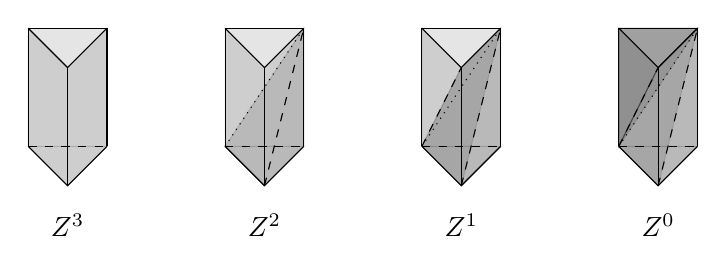
\begin{tikzpicture}[scale=0.5]
\draw (0,0) -- (1,-1) -- (2,0);
\draw[dashed] (0,0) -- (2,0);
\draw (0,3) -- (1,2) -- (2,3);
\draw (0,3) -- (2,3);
\draw (0,0) -- (0,3);
\draw (2,0) -- (2,3);
\draw (1,-1) -- (1,2);
\draw[fill, opacity=0.1] (0,0) -- (0,3) -- (1,2) -- (2,3) -- (2,0) -- (1,-1) -- cycle;
\draw[fill, opacity=0.1] (0,0) -- (2,0) -- (1,-1) -- cycle;
\draw[fill, opacity=0.1] (0,0) -- (2,0) -- (2,3) -- (0,3) --  cycle;


\draw (5,0) -- (6,-1) -- (7,0);
\draw[dashed] (5,0) -- (7,0);
\draw (5,3) -- (6,2) -- (7,3);
\draw (5,3) -- (7,3);
\draw (5,0) -- (5,3);
\draw (7,0) -- (7,3);
\draw (6,-1) -- (6,2);
\draw[fill, opacity=0.1] (5,0) -- (5,3) -- (6,2) -- (7,3) -- (7,0) -- (6,-1) -- cycle;
\draw[fill, opacity=0.1] (5,0) -- (7,0) -- (6,-1) -- cycle;
\draw[fill, opacity=0.1] (5,0) -- (7,0) -- (7,3) -- (5,3) --  cycle;
\draw[dashed] (6,-1) -- (7,3);
\draw[dotted] (5,0) -- (7,3);
\draw[fill, opacity=0.1] (5,0) -- (7,3) -- (7,0) -- (6,-1) --  cycle;



\draw (10,0) -- (11,-1) -- (12,0);
\draw[dashed] (10,0) -- (12,0);
\draw (10,3) -- (11,2) -- (12,3);
\draw (10,3) -- (12,3);
\draw (10,0) -- (10,3);
\draw (12,0) -- (12,3);
\draw (11,-1) -- (11,2);
\draw[fill, opacity=0.1] (10,0) -- (10,3) -- (11,2) -- (12,3) -- (12,0) -- (11,-1) -- cycle;
\draw[fill, opacity=0.1] (10,0) -- (12,0) -- (11,-1) -- cycle;
\draw[fill, opacity=0.1] (10,0) -- (12,0) -- (12,3) -- (10,3) --  cycle;
\draw[dashed] (11,-1) -- (12,3);
\draw[dotted] (10,0) -- (12,3);
\draw[fill, opacity=0.1] (10,0) -- (11,2) -- (12,3) -- (12,0) -- (11,-1) --  cycle;
\draw[fill, opacity=0.1] (10,0) -- (11,2) -- (12,3) -- (11,-1) --  cycle;
\draw[dashed] (10,0) -- (11,2);

\draw (15,0) -- (16,-1) -- (17,0);
\draw[dashed] (15,0) -- (17,0);
\draw (15,3) -- (16,2) -- (17,3);
\draw (15,3) -- (17,3);
\draw (15,0) -- (15,3);
\draw (17,0) -- (17,3);
\draw (16,-1) -- (16,2);
\draw[fill, opacity=0.1] (15,0) -- (15,3) -- (16,2) -- (17,3) -- (17,0) -- (16,-1) -- cycle;
\draw[fill, opacity=0.1] (15,0) -- (17,0) -- (16,-1) -- cycle;
\draw[fill, opacity=0.1] (15,0) -- (17,0) -- (17,3) -- (15,3) --  cycle;
\draw[dashed] (16,-1) -- (17,3);
\draw[dotted] (15,0) -- (17,3);
\draw[fill, opacity=0.1] (15,0) -- (16,2) -- (17,3) -- (17,0) -- (16,-1) --  cycle;
\draw[fill, opacity=0.1] (15,0) -- (16,2) -- (17,3) -- (16,-1) --  cycle;
\draw[dashed] (15,0) -- (16,2);
\draw[fill, opacity=0.3] (15,0) -- (15,3) -- (17,3) -- (16,2) --  cycle;
\draw[fill, opacity=0.1] (15,0) -- (16,2) -- (17,3) -- cycle;
\draw (1,-2) node{$Z^3$};
\draw (6,-2) node{$Z^2$};
\draw (11,-2) node{$Z^1$};
\draw (16,-2) node{$Z^0$};

\end{tikzpicture}
\caption{An illustration of \cref{prop:filtfill} when $n=2$}
\end{figure}













\section{Weak $\infty $-bicategories and $\infty $-bicategories} \label{sn:mainresult} In this section we aim to outline a proof that weak $\infty $-bicategories are $\infty $-bicategories, following the approach of Gagna, Harpaz and Lanari in \cite{GHL}.


\begin{thm}{\cite[Corollary 5.5]{GHL}}\label{weakbiop}
 For a scaled simplicial set $\overline{X} $, the following are equivalent.
 \begin{enumerate}[label={\normalfont(\arabic*)}]
  \item $\overline{X} $ is a weak $\infty $-bicategory.
 \item $\overline{X} ^{\emph{op} }$ is a weak $\infty $-bicategory.
 \item $\overline{X} $ is an $\infty $-bicategory.  
 \end{enumerate}
\end{thm}

We will prove \cref{weakbiop} in parts (see \cref{bicatwk}, \cref{prop:biop},  and \cref{wkbicat}). 
\begin{prop}\label{bicatwk}
 An $\infty $-bicategory is a weak $\infty $-bicategory.  
\end{prop}
\begin{proof}
	Scaled anodyne maps are trivial cofibrations in the bicategorical model structure (see \cite[Proposition 3.1.13]{GC}). Thus, $\infty $-bicategories, being fibrant objects in the bicategorical model structure, satisfy the extension condition with respect to all scaled anodyne maps.
\end{proof}

\begin{prop}\label{prop:biop}
 Bicategorical equivalences are op-invariant. Consequently, a scaled simplicial set is an $\infty $-bicategory if and only if its opposite is an $\infty $-bicategory. 
\end{prop}
\begin{proof}
 Using the necklace construction (see \cref{necklacethm1,necklacethm2}), for a simplicial set $X$ and vertices $x,y\in X_{0}$, we see that there is a natural isomorphism $\phi _{X}:\mathfrak{C}(X)(x,y)\rightarrow \mathfrak{C}(X^{\text{op} })(y,x)$ that takes each representative necklace triple to itself. It is not hard to check that this map is compatible with composition and that the maps $\mathfrak{C}(X)(x,y)\rightarrow \mathfrak{C}(X^{\text{op} })(y,x) \rightarrow  \mathfrak{C}((X^{\text{op}})^{\text{op} })(x,y)\cong \mathfrak{C}(X)(x,y)$ compose to give the identity map. Using the description of the scaled rigidification functor given in \cref{const:scnr}, it follows that $\phi _{X}$ preserves and detects marked edges and hence induces an isomorphisms of mapping marked simplicial sets. This implies that bicategorical equivalences are op-invariant. \end{proof}
To prove \cref{weakbiop}, it remains to be shown that a weak $\infty $-bicategory is an $\infty $-bicategory. We begin with the following proposition that is in similar vein to a familiar result in the Quillen model structure-- If $X\wkeq Y$ is a weak equivalence of topological spaces and the following diagram commutes, then there exists a map $\mathbb{D}^{n}\rightarrow X$  that makes the upper triangle commute and the lower triangle commute upto homotopy relative to $\mathbb{S}^{n}$. (See \cite[Proposition 7.6]{Hq} for a proof)
\[\begin{tikzcd}
	{\mathbb{S}^{n}} && {X} \\
	\\
	{\mathbb{D}^{n}} && {Y}
	\arrow[""', hook, from=1-1, to=3-1]
	\arrow["{\gamma'}"', from=3-1, to=3-3]
	\arrow["\wr", from=1-3, to=3-3]
	\arrow["\gamma", from=1-1, to=1-3]
\end{tikzcd}\]




\begin{prop}\label{quillenesque}
 Let $w:\overline{S}  \rightarrow \overline{T}  $ be a bicategorical equivalence of weak $\infty $-bicategories. Suppose that the following diagram commutes
% https://q.uiver.app/#q=WzAsNCxbMCwwLCJcXHBhcnRpYWwgXFxEZWx0YV5uX3tcXGZsYXR9Il0sWzAsMiwiXFxEZWx0YV5uX1xcZmxhdCJdLFsyLDIsIlxcb3ZlcmxpbmV7VH0iXSxbMiwwLCJcXG92ZXJsaW5le1N9Il0sWzAsMSwiaSIsMix7InN0eWxlIjp7InRhaWwiOnsibmFtZSI6Imhvb2siLCJzaWRlIjoidG9wIn19fV0sWzEsMiwiXFxnYW1tYSciLDJdLFszLDIsIkYiXSxbMCwzLCJcXGdhbW1hIl1d
\begin{equation}
\begin{tikzcd}
	{\partial \Delta^n_{\flat,2}} && {\overline{S}} \\
	\\
{\Delta^n_{\flat,2}} && {\overline{T}}
	\arrow["i"', hook, from=1-1, to=3-1]
	\arrow["{\gamma'}"', from=3-1, to=3-3]
	\arrow["w", from=1-3, to=3-3]
	\arrow["\gamma", from=1-1, to=1-3]
\end{tikzcd}
\end{equation}
Then, there exists a map $\overline{\gamma } :\Delta ^{n}_{\flat,2} \rightarrow \overline{S} $ of scaled simplicial sets such that $\overline{\gamma } \circ i=\gamma $ and there exists a natural transformation $\eta :\Delta ^{1}_{\flat,2}\times \Delta ^{n}_{\flat,2} \rightarrow  \overline{T} $ from $\gamma '$ to $w\circ \overline{\gamma } $ relative to $\partial \Delta ^{n}_{\flat,2}$.  
\end{prop}

\begin{proof}

Since $w$ is a bicategorical equivalence, for any two vertices $s,s'\in S_{0}$, the map $\text{Hom}^{\text{R} }_{\overline{S} }(s,s')\rightarrow  \text{Hom}^{\text{R} }_{\overline{T} }(w(s),w(s'))$ is an equivalence of $\infty $-categories and in particular, is essentially surjective. This clearly implies the assertion for when $n=1$. Assume that $n\geqslant 2$.

We shall carry out the proof in steps.\footnote{Each step is accompanied by heuristic diagrams that roughly illustrate parts of the argument when $n=2$. These are included only to aid the intuition of the reader and do not constitute an integral part of the argument} Let $x:=\gamma (0)$ and $y:=\gamma (n)$. As a notation remark, for a simplicial set $X$ and a scaled simplicial set $\overline{S} $, we shall not distinguish between maps $X_{\flat,2}\rightarrow \overline{S} $ of scaled simplicial sets and the corresponding maps $X\rightarrow S$ of simplicial sets (or similarly between $\overline{S} \rightarrow X_{\sharp,2}$ and $S \rightarrow X$).

\begin{enumerate}
	\item First, using \cref{movinglemma} (in the case $\emptyset\subseteq \partial \Delta ^{n}$), we get $H:(\Delta ^{1}\times \partial \Delta ^{n}, L_{\partial \Delta ^{n}}) \rightarrow \overline{S} $ such that $H|_{\Delta ^{\{ 1 \} }\times \partial \Delta ^{n}}=\gamma $. $H$  ``moves'' $\gamma $ to a map $\mu := H|_{\Delta ^{\{ 0 \} }\times \partial \Delta ^{n}}$ that is easier to deal with. In particular, \cref{movinglemma} guarantees that $\mu |_{\Delta ^{\{ 0,1,\ldots ,n-1 \} }}$ is constant. Hence, we can canonically think of $\mu $ as a map $\nu :\partial \Delta ^{n-1}\rightarrow \text{Hom}^{\text{R} }_{\overline{S}}(x,y)$.
\begin{center}
	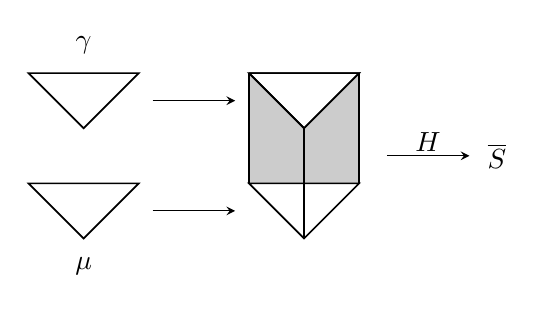
\begin{tikzpicture}[scale=0.7]
\draw[semithick] (1,0) -- (0,1) -- (2,1) -- cycle;
\draw[semithick] (0,3) -- (2,3) -- (1,2) -- cycle;
\draw[semithick] (5,0) -- (4,1) -- (6,1) -- cycle;
\draw[semithick] (4,3) -- (6,3) -- (5,2) -- cycle;
\draw[semithick] (4,1) -- (4,3);
\draw[semithick] (5,0) -- (5,2);
\draw[semithick] (6,1) -- (6,3);
\draw[semithick] (1,-0.5) node{$\mu$};
\draw[semithick] (1,3.5) node{$\gamma $};
\draw[semithick] (7.25,1.75) node{$H$};
\draw[fill, opacity=0.2] (4,1) -- (4,3) -- (5,2) -- (6,3) -- (6,1) -- (4,1);
\draw[semithick] (4,3) -- (5,2) -- (6,3) -- (4,3);
\draw[semithick] (8.5,1.5) node{$\overline{S}$};
\draw[-stealth] (2.25,0.5) -- (3.75,0.5);
\draw[-stealth] (2.25,2.5) -- (3.75,2.5);
\draw[-stealth] (6.5, 1.5) -- (8,1.5);
\end{tikzpicture}
\end{center}

 \item By assumption, $w\gamma $ extends to the $n$-cell $\gamma '$ in $T $. Applying \cref{movinglemma} (this time with respect to the inclusion $\partial \Delta ^{n}\subseteq \Delta ^{n}$) to the map $(\Delta ^{1}\times \partial \Delta ^{n},L_{\partial \Delta ^{n}})\bigsqcup _{\Delta ^{\{ 1 \} }_{\flat,2}\times \partial \Delta ^{n}_{\flat,2}} (\Delta ^{\{ 1 \} }_{\flat,2}\times \Delta ^{n}_{\flat,2})\xrightarrow{wH,\gamma '} \overline{T} $,  we obtain $H': (\Delta ^{1}\times \Delta ^{n}, L_{\Delta ^{n}})\rightarrow  \overline{T} $ that in particular, provides an extension $\mu ':=H'|_{\Delta ^{\{ 0 \} }\times \Delta ^{n}_{\flat,2}}$ of $w\mu $ to an $n$-cell . Again, \cref{movinglemma} guarantees that $\mu '|_{\Delta ^{\{ 0,1,\ldots ,n-1 \} }}$ is constant and we can canonically think of 
$\mu '$ as a map $\nu ':\Delta ^{n-1}\rightarrow \text{Hom} ^{\text{R} }_{\overline{T} }(w(x),w(y))$ that extends $w_{x,y}\circ \nu $, where $w_{x,y}$ denotes the map $\text{Hom}_{\overline{S}}^{\text{R} }(x,y) \rightarrow \text{Hom}^{\text{R} }_{\overline{T} }(w(x),w(y))$ induced by $w$.   


\begin{center}
	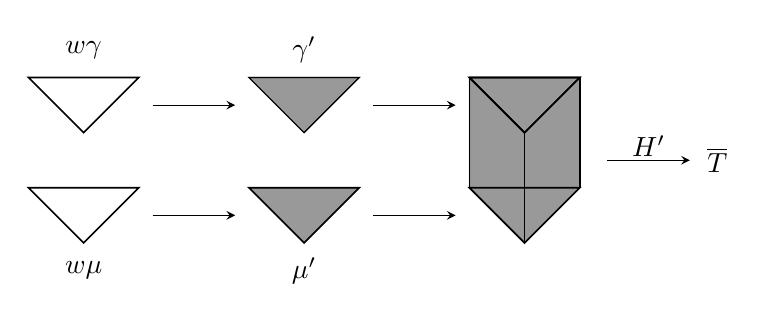
\begin{tikzpicture}[scale=0.7]
		\draw[fill, opacity=0.4] (1,0) -- (0,1) -- (2,1) -- cycle;
		\draw[fill, opacity=0.4] (0,3) -- (2,3) -- (1,2) -- cycle;
\draw[semithick] (1,0) -- (0,1) -- (2,1) -- cycle;
		\draw (0,3) -- (2,3) -- (1,2) -- cycle;

\draw[semithick] (5,0) -- (4,1) -- (6,1) -- cycle;
\draw[semithick] (4,3) -- (6,3) -- (5,2) -- cycle;
\draw[semithick] (4,1) -- (4,3);
\draw[semithick] (5,0) -- (5,2);
\draw[semithick] (6,1) -- (6,3);
\draw[semithick] (1,-0.5) node{$\mu'$};
\draw[semithick] (1,3.5) node{$\gamma'$};
\draw[semithick] (7.25,1.75) node{$H'$};
\draw[fill, opacity=0.4] (4,1) -- (4,3) -- (6,3) -- (6,1) -- (5,0) -- (4,1);
\draw[semithick] (4,3) -- (5,2) -- (6,3) -- (4,3);
\draw (8.5,1.5) node{$\overline{T}$};
\draw[-stealth] (2.25,0.5) -- (3.75,0.5);
\draw[-stealth] (2.25,2.5) -- (3.75,2.5);
\draw[-stealth] (6.5, 1.5) -- (8,1.5);
\draw[-stealth] (-1.75,0.5) -- (-0.25,0.5);
\draw[-stealth] (-1.75,2.5) -- (-0.25,2.5);
\draw[semithick] (-3,0) -- (-4,1) -- (-2,1) -- cycle;
\draw[semithick] (-3,2) -- (-4,3) -- (-2,3) -- cycle;
\draw[semithick] (-3,-0.5) node{$w\mu$};
\draw[semithick] (-3,3.5) node{$w\gamma$};

\end{tikzpicture}
\end{center}


 \item Consider the following commutative diagram. 
% https://q.uiver.app/#q=WzAsNCxbMCwwLCJbXFxEZWx0YV57bi0xfSxcXHRleHR7SG9tfV5cXHRleHR7Un1fe1xcb3ZlcmxpbmV7U319KHgseSldXlxcc2ltZXEiXSxbMCwyLCJbXFxwYXJ0aWFsXFxEZWx0YV57bi0xfSxcXHRleHR7SG9tfV5cXHRleHR7Un1fe1xcb3ZlcmxpbmV7U319KHgseSldXlxcc2ltZXEiXSxbMiwwLCJbXFxEZWx0YV57bi0xfSxcXHRleHR7SG9tfV5cXHRleHR7Un1fe1xcb3ZlcmxpbmV7VH19KHcoeCksdyh5KSldXlxcc2ltZXEiXSxbMiwyLCJbXFxwYXJ0aWFsXFxEZWx0YV57bi0xfSxcXHRleHR7SG9tfV5cXHRleHR7Un1fe1xcb3ZlcmxpbmV7VH19KHcoeCksdyh5KSldXlxcc2ltZXEiXSxbMCwxLCJpXipfe1xcdGV4dHtIb219XlxcdGV4dHtSfV97XFxvdmVybGluZXtTfX0oeCx5KX0iLDIseyJzdHlsZSI6eyJoZWFkIjp7Im5hbWUiOiJlcGkifX19XSxbMCwyLCJcXHNpbSJdLFsxLDMsIlxcc2ltIl0sWzIsMywiaV4qX3tcXHRleHR7SG9tfV5cXHRleHR7Un1fe1xcb3ZlcmxpbmV7VH19KHcoeCksdyh5KSl9IiwwLHsic3R5bGUiOnsiaGVhZCI6eyJuYW1lIjoiZXBpIn19fV1d
\[\begin{tikzcd}
{\underline{\textsf{sSet} } (\Delta^{n-1},\text{Hom}^\text{R}_{\overline{S}}(x,y))^\simeq} && {\underline{\textsf{sSet}}(\Delta^{n-1},\text{Hom}^\text{R}_{\overline{T}}(w(x),w(y)))^\simeq} \\
	\\
	{\underline{\textsf{sSet}} (\partial\Delta^{n-1},\text{Hom}^\text{R}_{\overline{S}}(x,y))^\simeq} && {\underline{\textsf{sSet} }(\partial\Delta^{n-1},\text{Hom}^\text{R}_{\overline{T}}(w(x),w(y)))^\simeq}
	\arrow["{i^*_{\text{Hom}^\text{R}_{\overline{S}}(x,y)}}"', two heads, from=1-1, to=3-1]
	\arrow["\sim", from=1-1, to=1-3]
	\arrow["\sim", from=3-1, to=3-3]
	\arrow["{i^*_{\text{Hom}^\text{R}_{\overline{T}}(w(x),w(y))}}", two heads, from=1-3, to=3-3]
\end{tikzcd}\]




The vertical maps are Kan fibrations by \cite[Proposition 4.4.5.3]{Ker} and since $w$ is a bicategorical equivalence, the horizontal maps are homotopy equivalences of Kan complexes by \cite[Proposition 4.5.1.22]{Ker}. Now, by \cite[Proposition 3.2.9.1]{Ker}, for any vertex in $\underline{\textsf{sSet} } (\partial \Delta ^{n-1},\text{Hom} _{S}^{\text{R} }(x,y))^{\simeq}$, the induced map on fibres is a homotopy equivalence of Kan complexes. In particular, the induced map on fibres corresponding to the vertex $\nu $ is essentially surjective. Hence there exists an extension $\overline{\nu } : \Delta ^{n-1} \rightarrow \text{Hom}_{\overline{S} }^{\text{R}}(x,y)$ of $\nu$ and an invertible natural transformation $\tilde{\eta }:\Delta ^{1} \times \Delta ^{n-1} \rightarrow  \text{Hom}_{\overline{T}}^{\text{R} }(w(x),w(y))$ relative to $\partial \Delta ^{n-1}$. This translates to an extension $\overline{\mu } $ of $\mu $ and an invertible natural transformation $\eta :\Delta ^{1}_{\flat,2} \times \Delta ^{n}_{\flat,2} \rightarrow  \overline{T} $ from $w\overline{\mu } $ to $\mu '$ relative to $\partial \Delta ^{n}_{\flat,2}$. 

\begin{center}
	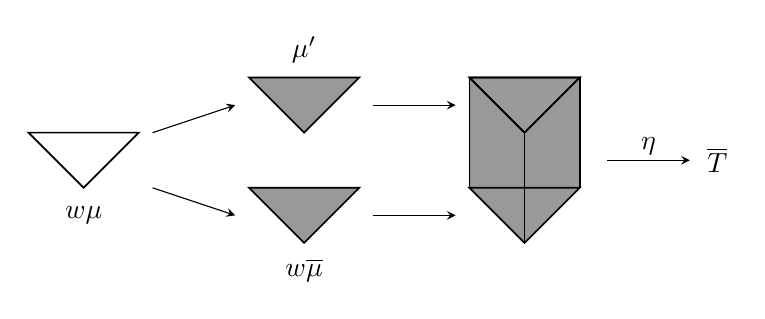
\begin{tikzpicture}[scale=0.7]
		\draw[fill, opacity=0.4] (1,0) -- (0,1) -- (2,1) -- cycle;
		\draw[fill, opacity=0.4] (0,3) -- (2,3) -- (1,2) -- cycle;
\draw[semithick] (1,0) -- (0,1) -- (2,1) -- cycle;
\draw[semithick] (0,3) -- (2,3) -- (1,2) -- cycle;

\draw[semithick] (5,0) -- (4,1) -- (6,1) -- cycle;
\draw[semithick] (4,3) -- (6,3) -- (5,2) -- cycle;
\draw[semithick] (4,1) -- (4,3);
\draw[semithick] (5,0) -- (5,2);
\draw[semithick] (6,1) -- (6,3);
\draw[semithick] (1,-0.5) node{$w\overline{\mu }$};
\draw[semithick] (1,3.5) node{$\mu '$};
\draw[semithick] (7.25,1.75) node{$\eta $};
\draw[fill, opacity=0.4] (4,1) -- (4,3) -- (6,3) -- (6,1) -- (5,0) -- (4,1);
\draw[semithick] (4,3) -- (5,2) -- (6,3) -- (4,3);
\draw[semithick] (8.5,1.5) node{$\overline{T}$};
\draw[-stealth] (2.25,0.5) -- (3.75,0.5);
\draw[-stealth] (2.25,2.5) -- (3.75,2.5);
\draw[-stealth] (6.5, 1.5) -- (8,1.5);
\draw[-stealth] (-1.75,1) -- (-0.25,0.5);
\draw[-stealth] (-1.75,2) -- (-0.25,2.5);
\draw[semithick] (-3,1) -- (-4,2) -- (-2,2) -- cycle;
\draw[semithick] (-3,0.5) node{$w\mu$};
\end{tikzpicture}
\end{center}


\item By \cref{prop:filtfill}, the map $(\Delta ^{1} \times \partial \Delta ^{n}, L_{\partial \Delta ^{n}})\bigsqcup_{ \Delta ^{\{ 0 \}}_{\flat,2} \times \partial \Delta ^{n}_{\flat,2}} (\Delta ^{\{ 0 \} }_{\flat,2}\times \Delta ^{n}_{\flat,2})\xrightarrow{H,\overline{\mu } } \overline{S} $ extends to a map
$\overline{H}:(\Delta ^{1}\times \Delta ^{n},L_{\Delta ^{n}}) \rightarrow \overline{S}  $. Define $\overline{\gamma }:=\overline{H}|_{\Delta ^{\{ 1 \} }_{\flat,2} \times \Delta ^{n}_{\flat,2}}$.
 
\begin{center}
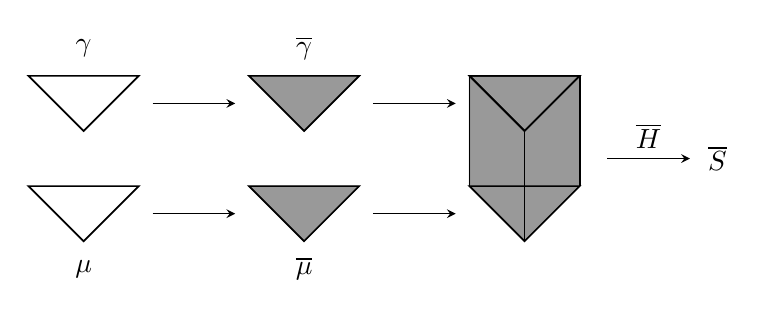
\begin{tikzpicture}[scale=0.7]
		\draw[fill, opacity=0.4] (1,0) -- (0,1) -- (2,1) -- cycle;
		\draw[fill, opacity=0.4] (0,3) -- (2,3) -- (1,2) -- cycle;
\draw[semithick] (1,0) -- (0,1) -- (2,1) -- cycle;
		\draw[semithick] (0,3) -- (2,3) -- (1,2) -- cycle;

\draw[semithick] (5,0) -- (4,1) -- (6,1) -- cycle;
\draw[semithick] (4,3) -- (6,3) -- (5,2) -- cycle;
\draw[semithick] (4,1) -- (4,3);
\draw[semithick] (5,0) -- (5,2);
\draw[semithick] (6,1) -- (6,3);
\draw[semithick] (1,-0.5) node{$\overline{\mu } $};
\draw[semithick] (1,3.5) node{$\overline{\gamma }$};
\draw[semithick] (7.25,1.9) node{$\overline{H} $};
\draw[fill, opacity=0.4] (4,1) -- (4,3) -- (6,3) -- (6,1) -- (5,0) -- (4,1);
\draw[semithick] (4,3) -- (5,2) -- (6,3) -- (4,3);
\draw[semithick] (8.5,1.5) node{$\overline{S}$};
\draw[-stealth] (2.25,0.5) -- (3.75,0.5);
\draw[-stealth] (2.25,2.5) -- (3.75,2.5);
\draw[-stealth] (6.5, 1.5) -- (8,1.5);
\draw[-stealth] (-1.75,0.5) -- (-0.25,0.5);
\draw[-stealth] (-1.75,2.5) -- (-0.25,2.5);
\draw[semithick] (-3,0) -- (-4,1) -- (-2,1) -- cycle;
\draw[semithick] (-3,2) -- (-4,3) -- (-2,3) -- cycle;
\draw[semithick] (-3,-0.5) node{$\mu $};
\draw[semithick] (-3,3.5) node{$\gamma$};

\end{tikzpicture}
\end{center}
\item Lastly, we show that this choice of $\gamma '$ works. Let $X= (\Delta ^{1} \times \partial \Delta ^{n}, L_{\partial \Delta ^{n}})\bigsqcup_{ \Delta ^{\{ 0 \}}_{\flat,2} \times \partial \Delta ^{n}_{\flat,2}} (\Delta ^{\{ 0 \} }_{\flat,2}\times \Delta ^{n}_{\flat,2})$ and $Y=(\Delta ^{1}\times \Delta ^{n}, L_{\Delta ^{n}})$. We have a map $\psi :(\Delta ^{1}_{\flat,2}\times X ) \bigsqcup_{\partial \Delta ^{1 }_{\flat,2} \times X} ( \partial \Delta ^{1}_{\flat,2}\times Y)\rightarrow \overline{S} $ such that
	\begin{enumerate}[label=(\roman*)]
		\item $\psi |_{\Delta ^{\{ 0 \}}_{\flat,2}\times Y}=H'$.
\item $\psi |_{\Delta ^{\{ 1 \} }_{\flat,2}\times Y}=w\overline{H} $.
 \item $\psi |_{\Delta ^{1}_{\flat,2}\times (\Delta ^{1}\times \partial \Delta ^{n}, L_{\partial \Delta ^{n}})}$ is the constant natural transformation.  \item $\psi |_{\Delta ^{1}_{\flat,2} \times (\Delta ^{\{ 0 \} }_{\flat,2}\times \Delta ^{n}_{\flat,2})}=\eta $.
 \end{enumerate}

	 Let $X'=X\bigsqcup_{(\Delta ^{1}\times \Delta ^{\{ 0 \} })} \Delta ^{0}$ and $Y'=Y\bigsqcup_{\Delta ^{1}\times \Delta ^{\{ 0 \} }} \Delta ^{0}$. Then, by \cref{prop:filtfill}, the inclusion $X'\rightarrow Y'$ is scaled anodyne. Further, by \cref{scbox}, the pushout product of this inclusion with the monomorphism $\partial \Delta ^{1}\rightarrow \Delta ^{1}$ is again scaled anodyne. This implies (due to (iii),(iv) of the definition of $\psi $) that $\psi $ extends to a map $\overline{\psi }:\Delta ^{1}_{\flat,2}\times Y \rightarrow  \overline{S} $ and the restriction $\overline{\psi }|_{\Delta ^{1}\times (\Delta ^{\{ 1 \} }\times \Delta ^{n})}$ is the required natural transformation from $\gamma '$ to $w\overline{\gamma } $.\footnote{indicated using a lighter shade in the following diagram}  
	 \begin{center}
		 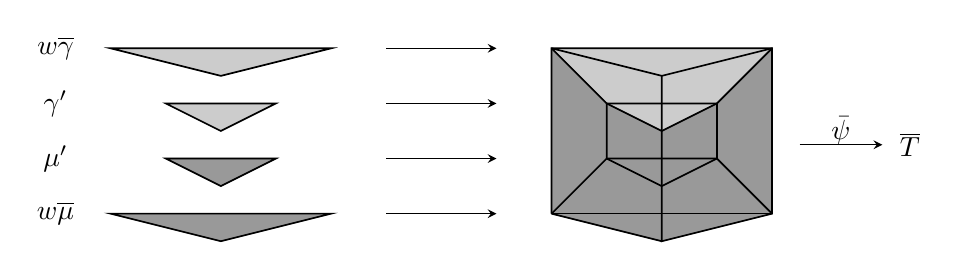
\begin{tikzpicture}[scale=0.7]
			 \draw[semithick] (0,0.5) -- (0,3.5) -- (4,3.5) -- (4,0.5) -- (2,0) -- (2,1) -- (3,1.5) -- (3,2.5) -- (1,2.5) -- (1,1.5) -- (2,1);
			 \draw[semithick] (0,0.5) -- (1,1.5) -- (3,1.5);
			 \draw[semithick] (2,1) -- (2,2) -- (2,3) -- (0,3.5);
			 \draw[semithick] (0,0.5) -- (4,0.5);
			 \draw[semithick] (2,3) -- (4,3.5);
			 \draw[semithick] (3,1.5) -- (4,0.5);
			 \draw[semithick] (0,0.5) -- (2,0);
			 \draw[semithick] (1,2.5) -- (2,2) -- (3,2.5);
			 \draw[semithick] (3,2.5) -- (4,3.5);
			 \draw[semithick] (0,3.5) -- (1,2.5);
			 \draw[-stealth] (4.5,1.75) -- (6,1.75);
			 \draw[fill, opacity=0.2] (0,3.5) -- (1,2.5) -- (2,2) -- (3,2.5) -- (4,3.5) -- (0,3.5);
			\draw[fill, opacity=0.4] (0,0.5) -- (0,3.5) -- (1,2.5) -- (2,2) -- (3,2.5) -- (4,3.5) -- (4,0.5) -- (2,0) -- (0,0.5);

			 \draw (6.5,1.75) node{$\overline{T} $};
			 \draw (5.25,2) node{$\bar{\psi} $};
			 \draw[semithick] (-8,3.5) -- (-6,3) -- (-4,3.5) -- cycle;
\draw[fill, opacity=0.2] (-8,3.5) -- (-6,3) -- (-4,3.5) -- cycle;
 \draw[semithick] (-8,0.5) -- (-6,0) -- (-4,0.5) -- cycle;
\draw[fill, opacity=0.4] (-8,0.5) -- (-6,0) -- (-4,0.5) -- cycle;
\draw[-stealth] (-3.0,3.5) -- (-1,3.5);
\draw[-stealth] (-3.0,0.5) -- (-1,0.5);
\draw[semithick] (-7,2.5) -- (-6,2) -- (-5,2.5) -- cycle;
\draw[fill,opacity=0.2] (-7,2.5) -- (-6,2) -- (-5,2.5) -- cycle;
\draw[semithick] (-7,1.5) -- (-6,1) -- (-5,1.5) -- cycle;
\draw[fill,opacity=0.4] (-7,1.5) -- (-6,1) -- (-5,1.5) -- cycle;
\draw[-stealth] (-3.0,1.5) -- (-1,1.5);
\draw[-stealth] (-3.0,2.5) -- (-1,2.5);
\draw (-9,3.5) node{$ w\overline{\gamma } $};
\draw (-9,2.5) node{$\gamma '$};
\draw (-9,1.5) node{$ \mu '$};
\draw (-9,0.5) node{$ w\overline{\mu } $};
		 \end{tikzpicture}
	 \end{center}
\end{enumerate}
 
\end{proof}







\begin{prop}\label{cylext}
 Let $w:\overline{S} \wkeq \overline{T} $ be a bicategorical equivalence of weak $\infty $-bicategories and $\overline{A} \hookrightarrow \overline{B} $ a cofibration of scaled simplicial sets. Suppose that the following diagram commutes and $\gamma '|_{\Delta ^{1}_{\flat,2}\times \overline{A}}$ is a pointwise invertible natural transformation.
% https://q.uiver.app/#q=WzAsNCxbMCwwLCJcXG92ZXJsaW5le0F9XFx0aW1lc1xcRGVsdGFee1xcezFcXH19X1xcZmxhdCJdLFswLDIsIihcXG92ZXJsaW5le0J9XFx0aW1lc1xcRGVsdGFee1xcezBcXH19X1xcZmxhdCkgXFxiaWdzcWN1cF97XFxvdmVybGluZXtBfVxcdGltZXNcXERlbHRhXntcXHswXFx9fV9cXGZsYXR9IChcXG92ZXJsaW5le0F9XFx0aW1lc1xcRGVsdGFeezF9X1xcZmxhdCkiXSxbMiwyLCJcXG92ZXJsaW5le1R9Il0sWzIsMCwiXFxvdmVybGluZXtTfSJdLFswLDEsIiIsMCx7InN0eWxlIjp7InRhaWwiOnsibmFtZSI6Imhvb2siLCJzaWRlIjoidG9wIn19fV0sWzEsMiwiXFxnYW1tYSciLDJdLFszLDIsInciXSxbMCwzLCJcXGdhbW1hIl1d
\[\begin{tikzcd}
	{\Delta ^{\{ 1 \} }_{\flat,2}\times \overline{A}} && {\overline{S}} \\
	\\
	{(\Delta ^{\{ 0 \} }_{\flat,2}\times \overline{B}) \bigsqcup_{\Delta ^{\{ 0 \} }_{\flat,2}\times \overline{A} } (\Delta ^{1}_{\flat,2}\times \overline{A})} && {\overline{T}}
	\arrow[hook, from=1-1, to=3-1]
	\arrow["{\gamma'}"', from=3-1, to=3-3]
	\arrow["w", from=1-3, to=3-3]
	\arrow["\gamma", from=1-1, to=1-3]
\end{tikzcd}\]
Then, the above diagram extends to the following commutative diagram 
where $\beta '$ is pointwise invertible.
% https://q.uiver.app/#q=WzAsNixbMCwwLCJcXG92ZXJsaW5le0F9XFx0aW1lc1xcRGVsdGFee1xcezFcXH19X1xcZmxhdCJdLFswLDIsIihcXG92ZXJsaW5le0J9XFx0aW1lc1xcRGVsdGFee1xcezBcXH19X1xcZmxhdCkgXFxiaWdzcWN1cF97XFxvdmVybGluZXtBfVxcdGltZXNcXERlbHRhXntcXHswXFx9fV9cXGZsYXR9IChcXG92ZXJsaW5le0F9XFx0aW1lc1xcRGVsdGFeezF9X1xcZmxhdCkiXSxbMiwyLCJcXG92ZXJsaW5le1R9Il0sWzIsMCwiXFxvdmVybGluZXtTfSJdLFsxLDAsIlxcb3ZlcmxpbmV7Qn1cXHRpbWVzXFxEZWx0YV57XFx7MVxcfX1fXFxmbGF0Il0sWzEsMiwiXFxvdmVybGluZXtCfVxcdGltZXMgXFxEZWx0YV4xX1xcZmxhdCJdLFswLDEsIiIsMCx7InN0eWxlIjp7InRhaWwiOnsibmFtZSI6Imhvb2siLCJzaWRlIjoidG9wIn19fV0sWzEsMiwiXFxnYW1tYSciLDIseyJsYWJlbF9wb3NpdGlvbiI6NjAsImN1cnZlIjo1fV0sWzMsMiwidyJdLFswLDMsIlxcZ2FtbWEiLDAseyJjdXJ2ZSI6LTV9XSxbMCw0LCIiLDIseyJzdHlsZSI6eyJ0YWlsIjp7Im5hbWUiOiJob29rIiwic2lkZSI6InRvcCJ9fX1dLFs0LDMsIlxcYmV0YSIsMl0sWzEsNSwiIiwwLHsic3R5bGUiOnsidGFpbCI6eyJuYW1lIjoiaG9vayIsInNpZGUiOiJ0b3AifX19XSxbNSwyLCJcXGJldGEnIl0sWzQsNSwiIiwxLHsic3R5bGUiOnsidGFpbCI6eyJuYW1lIjoiaG9vayIsInNpZGUiOiJ0b3AifX19XV0=
\[\begin{tikzcd}[cramped]
	{\Delta^{\{1\}}_{\flat,2} \times \overline{A} } & {\Delta^{\{1\}}_{\flat,2}\times \overline{B} } & {\overline{S}} \\
	\\
	{(\Delta^{\{0\}}_{\flat,2}\times \overline{B} ) \bigsqcup_{\Delta^{\{0\}}_{\flat,2} \times \overline{A} } (\Delta^{1}_{\flat,2} \times \overline{A} )} & { \Delta^1_{\flat,2} \times \overline{B} } & {\overline{T}}
	\arrow[hook, from=1-1, to=3-1]
	\arrow["{\gamma'}"'{pos=0.6}, curve={height=30pt}, from=3-1, to=3-3]
	\arrow["w", from=1-3, to=3-3]
	\arrow["\gamma", curve={height=-30pt}, from=1-1, to=1-3]
	\arrow[hook, from=1-1, to=1-2]
	\arrow["\beta"', from=1-2, to=1-3]
	\arrow[hook, from=3-1, to=3-2]
	\arrow["{\beta'}", from=3-2, to=3-3]
	\arrow[hook, from=1-2, to=3-2]
\end{tikzcd}\]




\end{prop}
\begin{rem}
We look at some ideas that naturally lead to the above proposition. Let $\mathcal{I} $ denote the collection of cofibrations $f: \overline{A} \hookrightarrow \overline{B} $ such that for every bicategorical equivalence $w:\overline{S} \wkeq \overline{T} $ of weak $\infty $-bicategories and a commutative square of the following form, there exists a map $h:\overline{B}  \rightarrow \overline{S}  $ such that $\gamma =h\circ f$.
\begin{equation}\label{cofcol}
% https://q.uiver.app/#q=WzAsNCxbMCwwLCJcXG92ZXJsaW5le0F9Il0sWzAsMiwiXFxvdmVybGluZXtCfSJdLFsyLDAsIlxcb3ZlcmxpbmV7U30iXSxbMiwyLCJcXG92ZXJsaW5le1R9Il0sWzAsMSwiZiIsMix7InN0eWxlIjp7InRhaWwiOnsibmFtZSI6Imhvb2siLCJzaWRlIjoidG9wIn19fV0sWzIsMywiXFx3ciJdLFsxLDMsIlxcZ2FtbWEnIiwyXSxbMCwyLCJcXGdhbW1hIl0sWzEsMiwiaCIsMCx7InN0eWxlIjp7ImJvZHkiOnsibmFtZSI6ImRhc2hlZCJ9fX1dXQ==
\begin{tikzcd}[cramped]
	{\overline{A}} && {\overline{S}} \\
	\\
	{\overline{B}} && {\overline{T}}
	\arrow["f"', hook, from=1-1, to=3-1]
	\arrow["w", from=1-3, to=3-3]
	\arrow["{\gamma'}"', from=3-1, to=3-3]
	\arrow["\gamma", from=1-1, to=1-3]
	\arrow["h", dashed, from=3-1, to=1-3]
\end{tikzcd}
\end{equation}
 In light of \cref{quillenesque}, we might hope to show that $\mathcal{I} $ is weakly saturated. Indeed, by \cref{quillenesque} and \cref{bicatdet}, the generating cofibrations given in \cref{gencofsc} are all contained in $\mathcal{I} $. Hence, proving that $\mathcal{I}$ is weakly saturated  would imply that $\mathcal{I} $ is precisely the collection of cofibrations. Assuming that this is true, the following diagram indicates that for any trivial cofibration $\overline{C} \tcof \overline{D} $ between weak $\infty $-bicategories, $\overline{C} $ is a retract of $\overline{D} $.
  % https://q.uiver.app/#q=WzAsNCxbMCwwLCJcXG92ZXJsaW5le0N9Il0sWzAsMiwiXFxvdmVybGluZXtEfSJdLFsyLDAsIlxcb3ZlcmxpbmV7Q30iXSxbMiwyLCJcXG92ZXJsaW5le0R9Il0sWzAsMSwiXFx3ciIsMCx7InN0eWxlIjp7InRhaWwiOnsibmFtZSI6Imhvb2siLCJzaWRlIjoidG9wIn19fV0sWzAsMiwiIiwyLHsib2Zmc2V0IjotMSwic3R5bGUiOnsiaGVhZCI6eyJuYW1lIjoibm9uZSJ9fX1dLFswLDIsIiIsMix7InN0eWxlIjp7ImhlYWQiOnsibmFtZSI6Im5vbmUifX19XSxbMSwzLCIiLDAseyJvZmZzZXQiOi0xLCJzdHlsZSI6eyJoZWFkIjp7Im5hbWUiOiJub25lIn19fV0sWzIsMywiXFx3ciIsMix7InN0eWxlIjp7InRhaWwiOnsibmFtZSI6Imhvb2siLCJzaWRlIjoidG9wIn19fV0sWzEsMywiIiwxLHsic3R5bGUiOnsiaGVhZCI6eyJuYW1lIjoibm9uZSJ9fX1dLFsxLDIsIiIsMSx7InN0eWxlIjp7ImJvZHkiOnsibmFtZSI6ImRhc2hlZCJ9fX1dXQ==
\[\begin{tikzcd}[cramped]
	{\overline{C}} && {\overline{C}} \\
	\\
	{\overline{D}} && {\overline{D}}
	\arrow["\wr", hook, from=1-1, to=3-1]
	\arrow[shift left, no head, from=1-1, to=1-3]
	\arrow[no head, from=1-1, to=1-3]
	\arrow[shift left, no head, from=3-1, to=3-3]
	\arrow["\wr"', hook, from=1-3, to=3-3]
	\arrow[no head, from=3-1, to=3-3]
	\arrow[dashed, from=3-1, to=1-3]
\end{tikzcd}\]
We may apply this to the fibrant replacement of a weak $\infty $-bicategory to conclude that a weak $\infty $-bicategory is indeed an $\infty $-bicategory.

It is easily seen that $\mathcal{I} $ is closed under retracts and pushouts. However, the ``routine argument'' to show that $\mathcal{I} $ is closed under compositions fails as the lower triangle of \cref{cofcol} does not commute in general. Alternatively, we could consider an improved version of this idea suggested by \cref{quillenesque} -- additionally require that the lower triangle is a natural transformation relative to $\overline{A}$. We rephrase the same idea as follows. We could consider the collection $\mathcal{J}$ of cofibrations $f:\overline{A}  \hookrightarrow  \overline{B}  $ of  scaled simplicial sets such that whenever \cref{cofcol} commutes such that $\gamma '|_{\Delta ^{1}_{\flat,2}\times \overline{A} }$ is the constant natural transformation, there exists an extension of the following form.
\begin{equation}\label{eq:factordiag2}
 \begin{tikzcd}[cramped]
	 {\overline{A}\times\Delta^{\{1\}}_{\flat,2}} & {\overline{B}\times\Delta^{\{1\}}_{\flat,2}} & {\overline{S}} \\
	\\
	{(\overline{B}\times\Delta^{\{0\}}_{\flat,2}) \bigsqcup_{\overline{A}\times\Delta^{\{0\}}_{\flat,2}} (\overline{A}\times\Delta^{1}_{\flat,2})} & {\overline{B}\times \Delta^1_{\flat,2}} & {\overline{T}}
	\arrow[hook, from=1-1, to=3-1]
	\arrow["{\gamma'}"'{pos=0.6}, curve={height=30pt}, from=3-1, to=3-3]
	\arrow["w", from=1-3, to=3-3]
	\arrow["\gamma", curve={height=-30pt}, from=1-1, to=1-3]
	\arrow[hook, from=1-1, to=1-2]
	\arrow["\beta"', from=1-2, to=1-3]
	\arrow[hook, from=3-1, to=3-2]
	\arrow["{\beta'}", from=3-2, to=3-3]
	\arrow[hook, from=1-2, to=3-2]
\end{tikzcd}
\end{equation}

Unfortunately, as before, the routine argument to show that $\mathcal{J} $ is closed under compositions fails for a similar reason -- we do not require the map $\beta '$ to be as strong as $\gamma '|_{\Delta ^{1}_{\flat,2}\times \overline{A} }$. 

Nevertheless, $\mathcal{I} $ (and also $\mathcal{J} $) does turn out to be the collection of all cofibrations. This can proved by considering those diagrams of the form \cref{cofcol} where $\gamma '|_{\Delta ^{1}_{\flat,2}\times \overline{A} }$ is pointwise invertible and prove the existence of a factorisation as in \cref{eq:factordiag2}  where $\beta '$ is pointwise invertible. This is essentially \cref{cylext}.
\end{rem}

To prove \cref{cylext}, we will need the following scaled analogue of Joyal's special outer horn lifting theorem whose proof is similar to that of  \cref{joyohl}.
















\begin{prop}{\cite[Lemma 5.2]{GHL}}\label{joyohl2}
	Let $\overline{C} $ and $\overline{D} $ be weak $\infty $-bicategories and let $w:\overline{C}  \rightarrow \overline{D}  $ be a map of scaled simplicial sets that satisfies the extension property with respect to generating scaled anodyne maps of type \hyperlink{scanod1}{\emph{(\texttt{SA1})}} and \hyperlink{scanod3}{\emph{(\texttt{SA3})}}. For $n\geqslant 2$, let $T$ be the collection of all triangles in $\Delta ^{n}$ that are degenerate or contain the edge $\langle 0,1 \rangle$. Let $T_{0}\subseteq T$ be the subset consisting of those triangles contained in $\Lambda _{0}^{n}$. Then, a lifting problem of the following form admits a solution provided that $f(\langle 0,1 \rangle )$ is an equivalence.
% https://q.uiver.app/#q=WzAsNCxbMCwwLCIoXFxMYW1iZGFebl8wLFRfMCkiXSxbMCwyLCIoXFxEZWx0YV5uLFQpIl0sWzIsMCwiXFxvdmVybGluZXtDfSJdLFsyLDIsIlxcb3ZlcmxpbmV7RH0iXSxbMCwxLCIiLDAseyJzdHlsZSI6eyJ0YWlsIjp7Im5hbWUiOiJob29rIiwic2lkZSI6InRvcCJ9fX1dLFswLDIsImYiXSxbMSwzLCJnIl0sWzIsMywicCJdXQ==
\[\begin{tikzcd}[cramped]
	{(\Lambda^n_0,T_0)} && {\overline{C}} \\
	\\
	{(\Delta^n,T)} && {\overline{D}}
	\arrow[hook, from=1-1, to=3-1]
	\arrow["f", from=1-1, to=1-3]
	\arrow["g", from=3-1, to=3-3]
	\arrow["w", from=1-3, to=3-3]
\end{tikzcd}\]
\end{prop}





\begin{proof}[Proof of \cref{cylext}]
 For notational ease, let us define for a cofibration $f:\overline{A}  \rightarrow \overline{B}$,  $M _{f}:=(\Delta ^{\{ 1 \} }_{\flat,2}\times \overline{B}) \bigsqcup_{\Delta ^{\{ 1 \} }\times \overline{A} } (\Delta ^{1}_{\flat,2}\times \overline{A} )$.  Let $\mathcal{I} $ denote the collection of cofibrations $\overline{A} \rightarrow \overline{B}$  between scaled simplicial sets for which the assertion is valid. It turns out that $\mathcal{I} $ is weakly saturated. This involves nothing more than diagram chasing but a good amount of it that we defer the proof to \cref{wksat}.
  
 By \cref{gencofsc}, it is sufficient to prove the assertion in the following cases
\begin{enumerate}[label=(\roman*)]
\item $\overline{A}  \hookrightarrow \overline{B} = \Delta ^{2}_{\flat,2} \hookrightarrow \Delta ^{2}_{\sharp,2}$
 \item  $\overline{A}  \hookrightarrow  \overline{B}=\partial \Delta ^{n}_{\flat,2} \hookrightarrow \Delta ^{n}_{\flat,2} $ for some $n\geqslant 0$.
\end{enumerate}
Let us consider case (i). Firstly, we observe that $\gamma '$ carries  any $2$-cell in $M_{f}$ that contains at least one of the edges $\Delta ^{\{ (0,0),(0,1)) \} }$, $\Delta ^{\{ (1,0),(1,1) \} }$ and $\Delta ^{\{ (2,0),(2,1) \} }$  to a scaled $2$-cell of $\overline{T} $. Borrowing notation from  \cref{prop:filtfill}, this implies that $\gamma '$ carries every $2$-cell in $Z^{3}$ to a scaled $2$-cell in $\overline{T} $. Working through the filtration in \cref{prop:filtfill}, we see that $\gamma '$ carries every $2$-cell in $Z_{0}$ to a scaled $2$-cell in $\overline{T} $. In other words, $\gamma '$ extends along $M_{f}\hookrightarrow \Delta ^{1}_{\flat,2}\times \Delta ^{2}_{\sharp,2}$. The assertion now follows from the fact that bicategorical equivalences detect scaled $2$-cells (cf. \cref{bicatdet}).

We now deal with case (ii). First, we consider the easy subcase when $\overline{A} \hookrightarrow \overline{B} =\emptyset \hookrightarrow \Delta ^{0}$. The existence of an invertible natural transformation $\pi '$ and a map $\pi $  that make the following diagram commute is immediate from the essential surjectivity of $w$. 

% https://q.uiver.app/#q=WzAsNixbMCwwLCJcXGVtcHR5c2V0Il0sWzAsMiwiXFxEZWx0YV4wX1xcZmxhdCJdLFsyLDAsIlxcRGVsdGFeMF9cXGZsYXQiXSxbMiwyLCJcXERlbHRhXjBfXFxmbGF0XFx0aW1lc1xcRGVsdGFeMV9cXGZsYXQgXFxjb25nIFxcRGVsdGFeMV9cXGZsYXQiXSxbNCwyLCJcXG92ZXJsaW5le1R9Il0sWzQsMCwiXFxvdmVybGluZXtTfSJdLFswLDFdLFswLDJdLFsxLDMsIlxcRGVsdGFee1xcezBcXH19Il0sWzMsNCwiXFxwaSciLDAseyJzdHlsZSI6eyJib2R5Ijp7Im5hbWUiOiJkYXNoZWQifX19XSxbNSw0LCJ3Il0sWzIsMywiXFxEZWx0YV57XFx7MVxcfX0iLDJdLFsyLDUsIlxccGkiLDAseyJzdHlsZSI6eyJib2R5Ijp7Im5hbWUiOiJkYXNoZWQifX19XSxbMCw1LCJcXGdhbW1hIiwwLHsiY3VydmUiOi00fV0sWzEsNCwiXFxnYW1tYSciLDIseyJjdXJ2ZSI6NH1dXQ==
\[\begin{tikzcd}[cramped]
	\emptyset && {\Delta^0_{\flat,2}} && {\overline{S}} \\
	\\
	{\Delta^0_{\flat,2}} && {\Delta^0_{\flat,2}\times\Delta^1_{\flat,2} \cong \Delta^1_{\flat,2}} && {\overline{T}}
	\arrow[from=1-1, to=3-1]
	\arrow[from=1-1, to=1-3]
	\arrow["{\Delta^{\{0\}}}", from=3-1, to=3-3]
	\arrow["{\pi'}", dashed, from=3-3, to=3-5]
	\arrow["w", from=1-5, to=3-5]
	\arrow["{\Delta^{\{1\}}}"', from=1-3, to=3-3]
	\arrow["\pi", dashed, from=1-3, to=1-5]
	\arrow["\gamma", curve={height=-24pt}, from=1-1, to=1-5]
	\arrow["{\gamma'}"', curve={height=24pt}, from=3-1, to=3-5]
\end{tikzcd}\]


Now, let $\overline{A} \hookrightarrow \overline{B} = \partial \Delta ^{n} \hookrightarrow \Delta ^{n}$ for some $n\geqslant 1$. Note that with respect to the notation used in \cref{prop:filtfill}, $Z^{n+1}=M_{f}$. By arguments discussed in \cref{prop:filtfill}, $\gamma $ can be extended to $Z^{1}$. Further, since $\gamma $ is pointwise invertible, by \cref{joyohl2} $\gamma $  can be extended further to $Z^{0}=\Delta ^{1}_{\flat,2}\times \Delta ^{n}_{\flat,2}$. Let us call this extension $\xi :Z^{0} \rightarrow \overline{T} $. We apply \cref{quillenesque} to the following diagram
% https://q.uiver.app/#q=WzAsNCxbMCwwLCJcXHBhcnRpYWwgXFxEZWx0YV5uIF9cXGZsYXQiXSxbMCwyLCJcXERlbHRhXm5fXFxmbGF0Il0sWzIsMCwiXFxvdmVybGluZXtTfSJdLFsyLDIsIlxcb3ZlcmxpbmV7VH0iXSxbMCwxLCIiLDAseyJzdHlsZSI6eyJ0YWlsIjp7Im5hbWUiOiJob29rIiwic2lkZSI6InRvcCJ9fX1dLFswLDIsIlxcZ2FtbWEiXSxbMiwzLCJ3Il0sWzEsMywiXFx4aV97XFxEZWx0YV57XFx7MVxcfX1cXHRpbWVzXFxEZWx0YV5uX1xcZmxhdH0iLDJdXQ==
\[\begin{tikzcd}[cramped]
	{\partial \Delta^n _{\flat,2}} && {\overline{S}} \\
	\\
	{\Delta^n_{\flat,2}} && {\overline{T}}
	\arrow["\gamma", from=1-1, to=1-3]
	\arrow[hook, from=1-1, to=3-1]
	\arrow["w", from=1-3, to=3-3]
	\arrow["{\xi_{\Delta^{\{1\}}\times\Delta^n_{\flat,2}}}"', from=3-1, to=3-3]
\end{tikzcd}\]
to derive a map $\pi :\Delta ^{n}_{\flat,2}\rightarrow \overline{S} $ such that the composition $\partial \Delta ^{n}_{\flat,2} \hookrightarrow \Delta ^{n}_{\flat,2}\xrightarrow{\pi } \overline{S}$ is equal to $\gamma $. Further, there exists a natural transformation $\eta $  relative to $\partial \Delta ^{n}_{\flat,2 }$ from $\xi |_{\Delta ^{\{ 1 \} }\times \Delta ^{n}_{\flat,2}}$ to $w\pi $. The idea is to glue $\eta $ and $\xi $ together to obtain $\pi '$. Note that for any monomorphism $\overline{C} \hookrightarrow \overline{C'} $ of scaled simplicial sets and a weak $\infty $-bicategory $\overline{U} $, the map $\underline{\textsf{msSet}_{2}}(\overline{C'} , \overline{U})\rightarrow \underline{\textsf{msSet}_{2}}(\overline{C} ,\overline{U} )$  is a fibration in the bicategorical model structure by adjunction and \cref{scbox}. Since $(\Lambda _{1}^{2})_{\flat,2}\rightarrow \Delta ^{2}_{\sharp,2}$ is scaled anodyne, there exists a solution $\psi$  to the following lifting problem
% https://q.uiver.app/#q=WzAsNSxbMCwwLCIoXFxMYW1iZGFeMl8xKV9cXGZsYXQiXSxbMCwyLCJcXERlbHRhXjJfXFxzaGFycCJdLFsyLDIsIlxcRGVsdGFeMSJdLFs0LDAsIltcXERlbHRhXm4sIFxcb3ZlcmxpbmV7U31dXntcXHRleHR7c2N9fSJdLFs0LDIsIltcXHBhcnRpYWxcXERlbHRhXm4sIFxcb3ZlcmxpbmV7U31dXntcXHRleHR7c2N9fSJdLFswLDFdLFsxLDIsIlxcc2lnbWFeMSJdLFswLDMsIlxceGksXFxldGEiXSxbMiw0LCJcXGdhbW1hJyJdLFszLDRdLFsxLDMsIlxccGknIiwwLHsic3R5bGUiOnsiYm9keSI6eyJuYW1lIjoiZGFzaGVkIn19fV1d
\[\begin{tikzcd}[cramped]
	{(\Lambda^2_1)_{\flat,2}} &&&& {\underline{\textsf{msSet}_{2}}(\Delta^n, \overline{S})} \\
	\\
	{\Delta^2_{\sharp,2}} && {\Delta^1} && {\underline{\textsf{msSet}_{2}}(\partial\Delta^n, \overline{S})}
	\arrow["{\xi,\eta}", from=1-1, to=1-5]
	\arrow[from=1-1, to=3-1]
	\arrow[from=1-5, to=3-5]
	\arrow["{\psi}", dashed, from=3-1, to=1-5]
	\arrow["{\sigma^1}", from=3-1, to=3-3]
	\arrow["{\gamma'}", from=3-3, to=3-5]
\end{tikzcd}\]
Put $\pi '=d_{1}(\psi )$. It is straightforward that $\pi $ and $\pi '$ satisfy the required properties.   
\end{proof}
























\begin{prop}\label{wkbicat}
 A weak $\infty $-bicategory $\overline{S} $ is also an $\infty $-bicategory.  
\end{prop}
\begin{proof}
 Let $\overline{S} \tcof \overline{T}\twoheadrightarrow \ast$ be a fibrant replacement of $\overline{S} $. Here, $\overline{T} $ is an $\infty $-bicategory and in particular, by \cref{bicatwk},  a weak $\infty $-bicategory. Applying \cref{cylext} to the following commutative diagram,

% https://q.uiver.app/#q=WzAsNSxbMCwwLCJcXG92ZXJsaW5le1N9XFx0aW1lcyBcXERlbHRhXntcXHsxXFx9fV97XFxmbGF0fSJdLFswLDIsIihcXG92ZXJsaW5le1R9XFx0aW1lcyBcXERlbHRhXntcXHsxXFx9fV97XFxmbGF0fSkgXFxiaWdzcWN1cF97XFxvdmVybGluZXtTfVxcdGltZXMgXFxEZWx0YV57XFx7MFxcfX1fe1xcZmxhdH19IChcXG92ZXJsaW5le1N9XFx0aW1lcyBcXERlbHRhXnsxfV97XFxmbGF0fSkiXSxbNCwyLCJcXG92ZXJsaW5le1R9Il0sWzQsMCwiXFxvdmVybGluZXtTfSJdLFsyLDIsIlxcb3ZlcmxpbmV7VH0gXFx0aW1lc1xcRGVsdGFfXFxmbGF0XntcXHsxXFx9fSJdLFswLDEsIiIsMCx7InN0eWxlIjp7InRhaWwiOnsibmFtZSI6Imhvb2siLCJzaWRlIjoidG9wIn19fV0sWzAsMywiXFxjb25nIl0sWzMsMiwiXFx3ciIsMCx7InN0eWxlIjp7InRhaWwiOnsibmFtZSI6Imhvb2siLCJzaWRlIjoidG9wIn19fV0sWzMsMl0sWzEsNF0sWzQsMiwiXFxjb25nIl1d
\[\begin{tikzcd}
	{\overline{S}\times \Delta^{\{1\}}_{\flat,2}} &&&& {\overline{S}} \\
	\\
	{(\overline{T}\times \Delta^{\{1\}}_{\flat,2}) \bigsqcup_{\overline{S}\times \Delta^{\{0\}}_{\flat,2}} (\overline{S}\times \Delta^{1}_{\flat,2})} && {\overline{T} \times\Delta_{\flat,2}^{\{1\}}} && {\overline{T}}
	\arrow[hook, from=1-1, to=3-1]
	\arrow["\cong", from=1-1, to=1-5]
	\arrow["\wr", hook, from=1-5, to=3-5]
	\arrow[from=1-5, to=3-5]
	\arrow[from=3-1, to=3-3]
	\arrow["\cong", from=3-3, to=3-5]
\end{tikzcd}\]
we obtain the following factorisation of the isomorphism $\overline{S}\times \Delta ^{\{ 1 \} }_{\flat,2} \xrightarrow{\cong} \overline{S} $ 

% https://q.uiver.app/#q=WzAsMyxbMCwwLCJcXG92ZXJsaW5le1N9XFx0aW1lcyBcXERlbHRhXjFfe1xcZmxhdH0iXSxbMiwwLCJcXG92ZXJsaW5le1R9XFx0aW1lcyBcXERlbHRhXjFfXFxmbGF0Il0sWzEsMSwiXFxvdmVybGluZXtTfSJdLFswLDFdLFswLDIsIlxcY29uZyIsMl0sWzEsMl1d
\[\begin{tikzcd}
	{\overline{S}\times \Delta^{\{1\}}_{\flat,2}} && {\overline{T}\times \Delta^{\{1\}}_{\flat,2}} \\
	& {\overline{S}}
	\arrow[from=1-1, to=1-3]
	\arrow["\cong"', from=1-1, to=2-2]
	\arrow[from=1-3, to=2-2]
\end{tikzcd}\]
Hence, $\overline{S} $ is a retract of $\overline{T} $, which is fibrant.
In other words, $\overline{S}\rightarrow \ast $ is a retract of the fibration $\overline{T} \rightarrow \ast$. Thus, $\overline{S}$ is fibrant.
\end{proof}


\section{Weak $\infty $-bicategories and $(\infty ,2)$-categories} \label{sn:mainresult2}
In this section, we will prove that weak $\infty $-bicategories are the same (see \cref{cor:wkinfinf2}) as $\infty $-bicategories, thereby completing the proofs of some of the statements in \cref{thm:consolidated1} that are yet to be justified.

\begin{prop}\label{prop:wkdeg}
	Let $\mathcal{C} $ be an $(\infty ,2)$-category. Let $n\geqslant 3$ and  $G: \Lambda _{0}^{n} \rightarrow \mathcal{C} $ such that $G(\langle 0,1,n \rangle )$ is thin and $G|_{\Delta ^{\{0,1\}}}$ is constant. Then, $G$ extends to an $n$-simplex of $\mathcal{C} $.        
\end{prop}
\begin{proof}
We shall show this by induction on $n$. Firstly, let $n=3$. We shall construct a map $H:\Lambda _{2}^{4} \rightarrow \mathcal{C}$ by inductively defining it on a filtration of simplicial subsets of $\Lambda _{2}^{4}$ defined below.
\begin{align*}
	F_{0}&=\delta _{2}^{3}(\Lambda _{0}^{3})\\
	F_{1}&=F_{0}\cup \Delta ^{\{ 0,1,2 \} }\cup \Delta ^{\{ 1,2,3 \} } \cup \Delta ^{\{ 0,2,4 \} }\\
F_{2}&=F_{1}\cup \Delta ^{\{0,1,2,3\}}\\
F_{3}&=F_{2}\cup \Delta ^{\{ 0,2,3,4 \}}\\
F_{4}&=F_{3}\cup \Delta ^{\{ 0,1,2,4 \} }\\
\end{align*}
Define $H|_{F_{0}}=G$ and $H|_{F_{1}}$ to be any extension of $H|_{F_{0}}$ such that $H|_{\Delta ^{\{ 0,1,2 \} }}$ is constant, $H(\langle0,2,4\rangle)$ is left-degenerate and $H(\langle1,2,3\rangle)$ is thin. Since $H(\langle0,1,2\rangle)$ is thin, there exists an extension $H|_{F_{2}}$  of $H|_{F_{1}}$ to $F_{2}$ and subsequently, since $H(\langle0,2,4\rangle)$ is left degenerate, there exists an extension $H|_{F_{3}}$ of $H|_{F_{2}}$ to $F_{3}$. Since $\text{Pith}(\mathcal{C} )$ is an $\infty $-category, using \cref{joyohl} on $H|_{\delta _3^{3}(\Lambda _{0}^{3})}$, there exists $H|_{F_{4}}$ extending $H|_{F_{3}}$ to $F_{4}$. Finally, since $H(\langle1,2,3\rangle)$ is thin, $H|_{F_{4}}$ extends to $H:\Lambda _{2}^{4} \rightarrow \mathcal{C} $ which in turn admits an extension $\tilde{H}:\Delta ^{4} \rightarrow \mathcal{C} $. The composition $\Delta ^{3}\xrightarrow{\delta _{2}} \Delta ^{4}\xrightarrow{\tilde{H}} \mathcal{C} $ is the required filler for $G$.

Let $n=k>3$ and suppose that the proposition holds true for all $3\leqslant n<k$. Let $S$ denote the collection of maps $H:X \rightarrow \mathcal{C} $ that satisfy the following conditions:
\begin{enumerate}
	\item $X$ is a simplicial subset of $\Lambda _{2}^{k+1}$ containing $\text{Im} (\Lambda _{0}^{k}\overset{\iota}{\hookrightarrow} \Delta ^{k}\xrightarrow{\delta _{2}} \Delta ^{k+1})$ and all $2$-cells of $\Lambda _{2}^{n+1}$. 
	\item 	$H|_{\text{Im}(\delta _{2}\circ \iota)}=G$ 
 \item $H|_{\Delta ^{\{ 0,1,2 \} }}$ is constant.
	 \item $H(\langle1,2,\alpha \rangle)$ is thin for all $2<\alpha \leqslant k+1$
	 \item $H(\langle0,2,k+1\rangle)$ is left-degenerate. 
\end{enumerate}
Let $N$ denote the collection of non-degenerate simplices of $\Lambda _{2}^{k+1}$. We endow $N$ with a total order $\leqslant $ where we define $\langle\alpha _{1},\ldots ,\alpha _{u}\rangle\leqslant \langle\beta _{1},\ldots ,\beta _{v} \rangle$ precisely when $u< v$ or $\alpha _{i}<\beta _{i}$ for the smallest $i$ (if it exists) such that $\alpha _{i}\neq \beta _{i}$. This induces a preorder\footnote{In general, this is only a preorder as there might exist more than one map in $S$ with the same domain} on $S$ given by $(H :X \rightarrow \mathcal{C} )\preceq (H':X' \rightarrow \mathcal{C})$ iff the smallest element (if it exists) of $(X^{\text{nd} }\setminus (X')^{\text{nd} })\cup ((X')^{\text{nd} }\setminus X^{\text{nd} })$ belongs to $X'$.
To show that $S$ is non-empty, we shall construct a certain element $\phi :F \rightarrow \mathcal{C}$ of $S$ in steps using a filtration of simplicial subsets defined below. Let
\begin{align*}
	F_{0}&=\Delta ^{\{ 0,1,2 \} }\\
 F_{1}&=F_{0}\cup \text{Im}(\Lambda _{0}^{k}\overset{\iota }{\hookrightarrow} \Delta ^{k}\xrightarrow{\delta _{2}}\Delta ^{k+1})  \\
F_{2}&=F_1 \cup \left( \bigcup_{2<r<k+1} \Delta ^{\{1,2, r \} }\right) \\
 F_{3}&=F_{2}\cup \Delta ^{\{ 0,2,k+1 \} }\\
 F_{4}&=F_{3}\cup \Delta ^{\{ 0,1,2,k+1 \} } \\
F_{5}&=F_4 \cup \left( \bigcup_{2< r_{1}<r_{2}\leqslant k+1} \Delta ^{\{1,2, r_{1},r_{2} \} }\right) \\
F&=F_5 \cup \left( \bigcup_{2<r<k+1} \Delta ^{\{0,1,2, r \} }\right) \\
\end{align*}
We suitably define $\phi $ as indicated below
\begin{enumerate}\addtocounter{enumi}{-1}
	\item Define $\phi|_{F_{0}}$ to be constant at $G(\langle0\rangle)$
	 \item Extend $\phi|_{F_{0}}$  to $F_{1}$ using the map $G$.
	 \item Extend $\phi|_{F_{1}}$  to $F_{2}$ such that $\phi (\langle1,2,r\rangle)$ for $2<r<k+1$ is thin. 	
 \item Extend $\phi|_{F_{2}}$  to $F_{3}$ by defining $\phi (\langle0,2,k+1\rangle)=s_{0}(\phi (\langle0,k+1\rangle))$ 
	 \item The previous definitions imply that $\phi(\Lambda ^{\{ 0,1,2,k+1 \} }_{0})\subseteq \text{Pith}(\mathcal{C} )$. Hence, by \cref{joyohl}, there exists an extension of $\phi |_{F_{3}}$ to $F_{4}$ such that $\phi (\langle1,2,k+1\rangle)$ is thin. 
	 \item By some choices of horn extensions (made possible by the induction hypothesis), $\phi |_{F_{4}}$ can be extended to $F_{5}$ and further yet to $F$. 
 \end{enumerate}
It is straightforward to check that $\phi \in S$. Since $S$ is non-empty, it is easily seen that $S$ has at least one maximal element, say $M: Y \rightarrow  \mathcal{C} $.

Suppose towards contradiction that $Y\neq \Lambda _{2}^{k+1}$. Let $\langle \Gamma \rangle\in N\setminus Y^{\text{nd} }$ be minimum. We consider the following exhaustive cases:

\begin{flushleft}
 \textsc{Case 1:} $\{0,1,2\}\subseteq  \Gamma $ 
\end{flushleft}
Define $Z$ to be the largest simplicial subset of $Y$ such that $Z^{\text{nd} }\subseteq Y^{\text{nd} }\setminus \{\langle\Gamma \setminus \{ 1 \} \rangle\}$. It is evident from the construction of $\phi $ that $|\Gamma |>3$.  By an inner horn extension, there exists an extension of $M|_{Z}$ to a map $M':Z\cup \Delta ^{\Gamma } \rightarrow \mathcal{C} $ in $S$ contradicting the maximality of $M$. 
\begin{flushleft}
 \textsc{Case 2:} $\{ 0,1,2 \} \cap  \Gamma =\{ 2 \} $ 
\end{flushleft}
If $\Gamma =\{ 2,3,\ldots ,k+1 \} $, then by left degeneracy of $M(\langle0,2,k+1\rangle)$, $M$ admits an extension $M':Y\cup \Delta ^{\{ 0 \}\cup \Gamma } \rightarrow \mathcal{C} $ in $S$ contradicting the maximality of $M$. Otherwise, by the induction hypothesis, $M$ admits an extension $M':Y \cup \Delta ^{\{ 1 \} \cup \Gamma  }\rightarrow \mathcal{C}  $ in $S$  again contradicting the maximality of $M$.  
\begin{flushleft}
 \textsc{Case 3:} $\{ 0,1,2 \} \cap \Gamma =\{ 0,2 \} $  or $\{ 0,1,2 \}\cap \Gamma = \{ 1,2 \} $ 
\end{flushleft}
\begin{flushleft}
 \emph{Subcase 3.1:} $\Gamma =\{ 1,2,\ldots ,k+1 \}$  
\end{flushleft}

Let $Z$ be the largest simplicial subset of $Y$ such that $Z^{\text{nd} }\subseteq Y^{\text{nd} }\setminus \{\langle 1,3,\ldots ,k+1 \rangle\}$. Now, $M|_{Z}$ extends to a map $M':M\cup \Delta ^{\{1,2,\ldots ,k+1\}} \rightarrow \mathcal{C} $ since $M(\langle 1,2,3 \rangle )$ is thin. Clearly, $M'$ is in $S$ again and contradicts the maximality of $M$.   

\begin{flushleft}
 \emph{Subcase 3.2:} $\Gamma =\{ 0,2,\ldots ,k+1 \}$  
\end{flushleft}

     Define $Z$ to be the largest simplicial subset of $Y$ such that $Z^{\text{nd} }\subseteq Y^{\text{nd} }\setminus \{\langle\Gamma \setminus \{ 0,1 \} \rangle\}$. By left degeneracy of $M(\langle 0,2,k+1\rangle)$, $M|_{Z}$ can be extended to a map $M':Z \cup \Delta ^{\Gamma }\rightarrow \mathcal{C}$ contradicting the maximality of $M$. 

\begin{flushleft}
 \emph{Subcase 3.3:} Subcases 3.1 and 3.2 do not hold
\end{flushleft}
 Again,  define $Z$ to be the largest simplicial subset of $Y$ such that $Z^{\text{nd} }\subseteq Y^{\text{nd} }\setminus \{\langle\Gamma \setminus \{ 0,1 \} \rangle\}$. By the induction hypothesis, $M|_{Z}$ can be extended to a map $M':Z\cup \Delta ^{\{ 1 \} \cup (\Gamma \setminus \{ 0 \} ) } \rightarrow \mathcal{C} $. It is easily verified that $M'\in S$. As $M'(\langle0,1,2\rangle)$ is thin, we may further extend $M'$ to a map $M'': Z\cup \Delta ^{\Gamma  \cup \{ 0,1 \} } \rightarrow \mathcal{C}  $ which again belongs to $S$. This is in contradiction to the maximality of $M$. 
\begin{flushleft}
 \textsc{Case 4:} $2\notin \Gamma $ 
\end{flushleft}
Then, $\Gamma = \{ 0,1,\ldots ,k+1 \} \setminus \{ 0,2 \} $. Let $Z$ be the largest simplicial subset of $Y$ such that for each $\sigma \in Z^{\text{nd} }$, $\sigma \leqslant \langle\Gamma \rangle$. Since $M(\langle0,2,k+1\rangle)$ is thin, there exists an extension of $M|_{Z}$ to a map $M':Z\cup \Delta ^{\{0,2,3\ldots ,k+1\}} \rightarrow \mathcal{C} $. Since $M'(\langle0,1,2\rangle)$ is thin, $M'$ can be further extended to a map $M'':Z\cup \Delta ^{\{ 0,2,3,\ldots ,k+1 \} }\cup \Delta ^{\{ 1,2,3,\ldots ,k+1 \} } \rightarrow \mathcal{C} $. Clearly, $M''\in S$ and contradicts the maximality of $M$. 

Hence, $M:\Lambda _{2}^{k+1} \rightarrow \mathcal{C} $. As $M\in S$, $M(\langle1,2,3\rangle)$ is thin and $M$ extends to a $(k+1)$-cell $\tau$ of $\mathcal{C} $. The composition $\Delta ^{k}\xrightarrow{\delta _{2}} \Delta ^{k+1}\xrightarrow{\tau} \mathcal{C} $ acts as a filler for $G$.
      
\end{proof}
\begin{prop}\label{prop:inf2weak}
 If $\mathcal{C}$ is an $(\infty,2)$-category, then $(\mathcal{C} ,\emph{thin}(\mathcal{C} ))$ is a weak $\infty $-bicategory.  
\end{prop}
\begin{proof}
$(\mathcal{C} ,\text{thin}(\mathcal{C} ))$ satisfies the extension property with respect to maps in \hyperlink{scanod1}{(\texttt{SA1})} by definition of thin $2$-cells and since $\mathcal{C} $ satisfies \hyperlink{inf2cat1}{(\texttt{I1})}. Extension against maps in \hyperlink{scanod2}{(\texttt{SA2})} can be derived using \cref{innerexch} and \cref{fourfive}. Lastly, by \cref{prop:wkdeg}, $(\mathcal{C}, \text{thin}(\mathcal{C}))$  satisfies the extension property with respect to maps in \hyperlink{scanod3}{(\texttt{SA3})}.
\end{proof}
\begin{prop}\label{prop:thinscal}
 Let $\overline{X} $ be a weak $\infty $-bicategory. Then, a $2$-cell in $X$ is scaled if and only if it is thin.  
\end{prop}
\begin{proof}
Clearly, every scaled $2$-cell in a weak $\infty $-bicategory is thin. Conversely, let $\gamma $ be a thin $2$-cell in $X$. Let $\gamma '$ be a scaled $2$-cell such that the horn inclusion $\Lambda _{1}^{2}\hookrightarrow \Delta ^{2}$ equalises $\gamma $ and $\gamma '$. It is not hard to construct a $4$-cell $\tau\in X_{4}$ satisfying the following properties
\begin{enumerate}[label=(\roman*)]
 \item $\tau\circ \delta _{4}^{4}=(\gamma \circ \delta^{2} _{2})\circ (\sigma^{1} _{0}\circ \sigma^{2} _{0})$
 \item $\tau \circ \delta^{4} _{2}\circ \delta^{3} _{0}=\gamma '$
 \item $\tau\circ \delta _{1}^{4} = \gamma \circ \sigma _{0}^{2}$
\end{enumerate}
It follows from \hyperlink{scanod2}{(\texttt{SA2})} that $\gamma $ is also scaled.  
\end{proof}

\begin{prop}\label{weakinf2}
 If $\overline{X}$ is a weak $\infty $-bicategory, then $X$ is an $(\infty ,2)$-category. 
\end{prop}
\begin{proof}
 Follows immediately from \cref{prop:thinscal} and \cref{weakbiop}.
\end{proof}


We summarise the results of this section as follows.
\begin{cor}\label{cor:wkinfinf2}
We have the following canonical bijective correspondence.
\begin{align*}
	\{ \text{Weak } \infty\text{-bicategories }\} &\leftrightarrow \{ (\infty ,2)\text{-categories }\} \\
 \overline{X} &\mapsto X\\
 (Y,{\emph{thin} }(Y))&\mapsfrom Y
\end{align*}
\end{cor}


















































\section{Bicategorical Equivalences}\label{4.8}
Summarising, we have the following equivalent descriptions of fibrant objects in $\textsf{msSet}_{2}$. We will use these descriptions interchangeably.
		\begin{enumerate}
			\item $\overline{S} $ is an $\infty $-bicategory (\cref{defn:infbicat}).
			\item $\overline{S} $ is a weak $\infty $-bicategory (\cref{defn:weakinfbicat}).
			\item $S$ is an $(\infty,2)$-category (\cref{defn:inf2cat}) and $\overline{S}=(S,\text{thin}(S))$.  
	\end{enumerate}



In this section, we extend \cref{bicatlocal}, providing two more equivalent formulations along the lines of \cref{prop:infequiv}, which we recall here. 

\begin{rec}
 The following are equivalent for a map $F:X \rightarrow Y$ of $\infty $-categories.   
 \begin{enumerate}[label=\normalfont(\arabic*)]
	 \item $\mathfrak{C}(F)$ is a weak equivalence in $\emph{\textsf{sSet}\text{-}\textsf{Cat}}$.  
 \item $F$ is fully faithful and essentially surjective.
 \item $F$ is an $E$-homotopy equivalence. That is, there exists a functor $G:Y \rightarrow X$ of $\infty $-categories such that $\emph{Id}_{X}$ is $E$-homotopic to $GF$ and $\emph{Id}_{Y}$ is $E$-homotopic to $FG$.
 \item $F$ is a categorical equivalence. That is, $(F^{*})^{\simeq}:\underline{\emph{\textsf{sSet}}} (Y,Z)^{\simeq}\rightarrow \underline{\emph{\textsf{sSet}}}(X,Z)^{\simeq}$ is a homotopy equivalence of Kan complexes for every $\infty $-category $Z$.  
\end{enumerate}
\end{rec}

\begin{rem}
In the proof of \cref{bequiv}, for scaled simplicial sets $\overline{S}$ and $\overline{T} $, by abuse of notation, we at times write $\underline{\textsf{msSet}_{2}}(\overline{S},\overline{T})$ to denote its underlying simplicial set.   
\end{rem}




\begin{prop}\label{bequiv}
 The following are equivalent for a functor $F:\mathcal{C}  \rightarrow \mathcal{D}  $ of $(\infty ,2)$-categories.
 \begin{enumerate}[label={\normalfont (\arabic*)}]
	 \item $F$ is a bicategorical equivalence. That is, $\mathfrak{C}^{\emph{sc}}(F)$ is a weak equivalence in $\emph{\textsf{msSet}}_{1}\emph{\text{-}\textsf{Cat}}$
\item For any two vertices $c_0,c_1$ in $\mathcal{C} $, $\emph{Hom}_{\mathcal{C} }^{\emph{R}}(c_0,c_1)\rightarrow \emph{Hom}_{\mathcal{D} }^{\emph{R}}(Fc_0,Fc_1)$ is an equivalence of $\infty $-categories and for any vertex $d$ of $\mathcal{D} $, there exists a vertex $c$ of $\mathcal{C} $ such that there exists an equivalence $F(c)\rightarrow d$.
	 \item For any two vertices $c_0,c_1$ in $\mathcal{C} $, $\emph{Hom}_{\mathcal{C} }^{\emph{L}}(c_0,c_1)\rightarrow \emph{Hom}_{\mathcal{D} }^{\emph{L}}(Fc_0,Fc_1)$ is an equivalence of $\infty $-categories and for any vertex $d$ of $\mathcal{D} $, there exists a vertex $c$ of $\mathcal{C} $ such that there exists an equivalence $F(c)\rightarrow  d$.
	 \item There exist maps $G:\mathcal{D}  \rightarrow \mathcal{C}  $, $H :E \times \mathcal{C}  \rightarrow  \mathcal{C} $ and $H':E  \times \mathcal{D}  \rightarrow  \mathcal{D} $ of $\infty $-bicategories such that
		 \begin{enumerate}[label={\normalfont (\roman*)}]
		  \item $H|_{\{ 0 \} \times \mathcal{C} }=\emph{Id}_{\mathcal{C} }$
\item $H|_{\{ 1 \} \times \mathcal{C} }= GF$
\item $H'|_{\{ 0 \} \times \mathcal{D} }=\emph{Id}_{\mathcal{D} }$
\item $H'|_{\{ 1 \} \times \mathcal{D} }=FG$
		 \end{enumerate}
	 \item $\emph{Pith}(F^{*}):\emph{Pith}(\underline{\emph{\textsf{msSet}}_{2}}(\mathcal{D} ,\mathcal{E})) \rightarrow \emph{Pith}(\underline{\emph{\textsf{msSet}}_{2}}(\mathcal{C},\mathcal{E}))$ is an equivalence of $\infty $-categories for every $(\infty ,2)$-category $\mathcal{E} $. 
 \end{enumerate}

\end{prop}

\begin{proof}
	\flushleft{(1) $\Leftrightarrow $ (2)}\quad See \cref{bicatlocal}.
	\flushleft{(2) $\Leftrightarrow$ (3)} This follows from \cref{weakbiop} and \cref{rem:bequivop}.
	\flushleft{(1) $\Leftrightarrow $ (4)}\quad  For any $(\infty ,2)$-category $\mathcal{E} $, $E\times \mathcal{E} $ is a cylinder object for $\mathcal{E}$ (see \cref{thm:consolidated1}). Since $(\infty ,2)$-categories are bifibrant objects in the bicategorical model structure, statement (4) essentially says that $F$ is a homotopy equivalence in the bicategorical model structure. By \cref{prop:whitehead}, we have (1) $\Leftrightarrow$ (4). 
\flushleft{(4) $\Rightarrow $ (5)} \quad Let $G: \mathcal{D} \rightarrow \mathcal{C}  $ and $H':E\times \mathcal{D}  \rightarrow \mathcal{D}$ be as described in (4). For scaled simplicial sets $\overline{X},\overline{Y}$, let $\varepsilon _{\overline{Y},\overline{X}}: \overline{X}\times \underline{\textsf{msSet}_{2}}(\overline{X},\overline{Y})\rightarrow  \overline{Y}$ denote the component corresponding to $\overline{X}$ of the counit of the adjunction $(\_\times \overline{Y}) \dashv \underline{\textsf{msSet}_{2}}(\overline{Y},\_)$. By adjunction, the composition $$(E\times \mathcal{D}) \times  \underline{\textsf{msSet}_{2}}(\mathcal{D},\mathcal{E} )\xrightarrow{H'\times \text{Id}} \mathcal{D}\times \underline{\textsf{msSet}_{2}}(\mathcal{D},\mathcal{E} ) \xrightarrow{\varepsilon _{\mathcal{E}  , \mathcal{D} }} \mathcal{E} $$ corresponds to a functor $\phi :E \times \underline{\textsf{msSet}_{2}}(\mathcal{D} ,\mathcal{E} )\rightarrow \underline{\textsf{msSet}_{2}}(\mathcal{D} ,\mathcal{E} )$ of $(\infty ,2)$-categories satisfying $\phi |_{\{ 0 \} \times \underline{\textsf{msSet}_{2}}(\mathcal{D} ,\mathcal{E} )}=\text{Id}_{\underline{\textsf{msSet}_{2}}(\mathcal{D} ,\mathcal{E} )}$ and $\phi |_{\{ 1 \} \times \underline{\textsf{msSet}_{2}}(\mathcal{D} ,\mathcal{E} )}=G^{*}F^{*}$. Similarly, we can construct 
$\psi :E_{}\times \underline{\textsf{msSet}_{2}}(\mathcal{C},\mathcal{E} ) \rightarrow \underline{\textsf{msSet}_{2}}(\mathcal{C} ,\mathcal{E} )$ satisfying $\psi |_{\{ 0 \} \times \underline{\textsf{msSet}_{2}}(\mathcal{C} ,\mathcal{E} )}=\text{Id}_{\underline{\textsf{msSet}_{2}}(\mathcal{C} ,\mathcal{E} )}$ and $\psi |_{\{ 1 \} \times \underline{\textsf{msSet}_{2}}(\mathcal{C} ,\mathcal{E} )}=F^{*}G^{*}$. Now, $\text{Pith}(\phi ):E\times \text{Pith}(\underline{\textsf{msSet}_{2}}(\mathcal{D},\mathcal{E} ))\rightarrow \text{Pith}(\underline{\textsf{msSet}_{2}}(\mathcal{D},\mathcal{E} ))$  and $\text{Pith}(\psi ):E\times \text{Pith}(\underline{\textsf{msSet}_{2}}(\mathcal{C},\mathcal{E} )) \rightarrow  \text{Pith}(\underline{\textsf{msSet}_{2}}(\mathcal{C},\mathcal{E}  ))$ 
satisfy the following 
\begin{align*}
	\text{Pith}(\phi )|_{\{ 0 \} \times \text{Pith}(\underline{\textsf{msSet}_{2}}(\mathcal{D},\mathcal{E} )) }&=\text{Id}_{\underline{\textsf{msSet}_{2}}(\mathcal{D},\mathcal{E}  )}\\
	\text{Pith}(\phi )|_{\{ 1 \} \times \text{Pith}(\underline{\textsf{msSet}_{2}}(\mathcal{D},\mathcal{E} )) }&= \text{Pith}(G^{*})\text{Pith}(F^{*})\\ 
	\text{Pith}(\phi )|_{\{ 0 \} \times \text{Pith}(\underline{\textsf{msSet}_{2}}(\mathcal{C} , \mathcal{E} )) }&=\text{Id}_{\underline{\textsf{msSet}_{2}}(\mathcal{C},\mathcal{E}  )}\\
\text{Pith}(\phi )|_{\{ 1 \} \times \text{Pith}(\underline{\textsf{msSet}_{2}}(\mathcal{C},\mathcal{E} )) }&= \text{Pith}(F^{*})\text{Pith}(G^{*})\\ 
\end{align*}
Thus, $\text{Pith}(F^{*})$ is an equivalence of $\infty $-categories.  
\flushleft{(5) $\Rightarrow $ (4)}\quad Suppose that for every $(\infty ,2)$-category $\mathcal{E} $,   $\text{Pith}(F^{*}):\text{Pith}(\underline{\textsf{msSet}_{2}}(\mathcal{D},\mathcal{E}))\rightarrow \text{Pith}(\underline{\textsf{msSet}_{2}}(\mathcal{C},\mathcal{E})) $ is an equivalence $\infty $-categories. Then, $\chi _{\mathcal{E} }:=\pi _{0}(\text{Pith}(F^{*})^{\simeq}):\pi _{0}(\text{Pith}(\underline{\textsf{msSet}_{2}}(\mathcal{D} ,\mathcal{E} ))^\simeq) \rightarrow \pi _{0}(\text{Pith}(\underline{\textsf{msSet}_{2}}(\mathcal{D} ,\mathcal{E}))^\simeq)$ is a bijection of sets for every $(\infty ,2)$-category $\mathcal{E} $. Since $\chi _{\mathcal{C} }$ is surjective, there exists $G\in \text{Pith}(\underline{\textsf{msSet}_{2}}(\mathcal{D},\mathcal{E}))^{\simeq}_{0}$ such that $\chi_{\mathcal{C} }(G)=[\text{Id} _{\mathcal{C}} ]$. In other words, there exists $a: E \rightarrow \text{Pith} (\underline{\textsf{msSet}_{2}}(\mathcal{C},\mathcal{C} ))$
such that $a(0)=\text{Id}_{\mathcal{C} }$ and $a(1)=GF$. Now, consider the composition
\begin{align*}
	E \xrightarrow{\text{Id}_{F},a} \text{Pith}(\underline{\textsf{msSet}_{2}}(\mathcal{C},\mathcal{D} )) &\times  \text{Pith}(\underline{\textsf{msSet}_{2}}(\mathcal{C},\mathcal{C})) \\ & \cong \\ \text{Pith}(\underline{\textsf{msSet}_{2}}(\mathcal{C},\mathcal{D} ) &\times \underline{\textsf{msSet}_{2}}(\mathcal{C},\mathcal{C} )) \xrightarrow{\text{Pith}(c_{\mathcal{\mathcal{D} ,\mathcal{C} ,\mathcal{C} } })} \text{Pith}(\underline{\textsf{msSet}_{2}} (\mathcal{C},\mathcal{D} ))  
\end{align*}
which maps vertices $0$ and $1$ of $E$ to $F$ and $FGF$ respectively. Here, $c_{\mathcal{D},\mathcal{C},\mathcal{C} }$ refers to the composition map that is part of the enriched structure. This implies that $[F]=[FGF]$ in $\pi _{0}(\text{Pith}(\underline{\textsf{msSet}_{2}}(\mathcal{C},\mathcal{D} ))^{\simeq})$. Thus, by injectivity of $\chi _{\mathcal{D} }$, there exists $a':E\rightarrow \text{Pith}(\underline{\textsf{msSet}_{2}}(\mathcal{D},\mathcal{D}))$ such that $a'(0)=\text{Id}_{\mathcal{D} }$ and $a'(1)=FG$. By adjunction, $a$ and $a'$ correspond to maps $H:E \rightarrow \underline{\textsf{msSet}_{2}}(\mathcal{C},\mathcal{C})$ and $H': E \rightarrow \underline{\textsf{msSet}_{2}} (\mathcal{D} ,\mathcal{D} ) $ of $(\infty ,2)$-categories. It is immediate that $G,H$ and $H'$ as constructed satisfy (4).        
\end{proof}




















\newpage
\chapter{$\infty $-Preorders and Locally $0$-Truncated $\infty $-Categories }\label{preloc}

\tikzset{
    ncbar angle/.initial=90,
    ncbar/.style={
        to path=(\tikztostart)
        -- ($(\tikztostart)!#1!\pgfkeysvalueof{/tikz/ncbar angle}:(\tikztotarget)$)
        -- ($(\tikztotarget)!($(\tikztostart)!#1!\pgfkeysvalueof{/tikz/ncbar angle}:(\tikztotarget)$)!\pgfkeysvalueof{/tikz/ncbar angle}:(\tikztostart)$)
        -- (\tikztotarget)
    },
    ncbar/.default=0.5cm,
}

\tikzset{square left brace/.style={ncbar=0.5cm}}
\tikzset{square right brace/.style={ncbar=-0.5cm}}

\tikzset{round left paren/.style={ncbar=0.5cm,out=120,in=-120}}
\tikzset{round right paren/.style={ncbar=0.5cm,out=60,in=-60}}


In this chapter, we study locally $n$-truncated $\infty $-categories for $n=-1,0$ and show that $(\infty ,2)$-categories representative of their homotopy theories are homotopy equivalent to those representing preorders and categories respectively. 

\section{Definitions}\label{preloc2}

\begin{defn}\label{defn:truncatedkc}
	Let $K$ be a Kan complex. For $n\geqslant 0$, $K$ is said to be $n$-\emph{truncated} if $\pi _{m}(K)$ is trivial for all $m>n$ (for any choice of basepoint). It is convenient to say that 
\begin{enumerate}
	\item $K$ is $(-1)$-\emph{truncated} if it is either empty or contractible.
	\item $K$ is $(-2)$-\emph{truncated} if it is contractible (and non-empty). 
\end{enumerate}
\end{defn}


\begin{defn}\label{defn:truncinf}
	For $n\geqslant 0$, an $\infty $-category $S$ is said to be \emph{locally} $n$-\emph{truncated} if for all $a,b\in S_{0}$, $\text{Hom}^{\text{L} }_{S}(a,b)$ is $n$-truncated. Locally $(-1)$-truncated $\infty $-categories will be called $\infty $-\emph{preorders}. For $n\geqslant -2$, let $\mathcal{T}^{n}$ denote the full subcategory of $\textsf{sSet}$ consisting of locally $n$-truncated $\infty $-categories.    
\end{defn}

\begin{defn}\label{defn:POtranslated}
 Let $\overline{\textsf{PO}}$ (resp. $\overline{\textsf{Cat}}$) denote the full subcategory of $\textsf{sSet}$ consisting of the nerves of small preorder categories (resp.  small categories).
\end{defn}
\begin{rem}
	We shall regard $\mathcal{T}^{-1}$, $\overline{\textsf{PO}}$, $\mathcal{T}^{0}$ and $\overline{\textsf{Cat}}$ as simplicial categories with the $\textsf{sSet}$-structure derived from the internal hom in $\textsf{sSet} $. Note that for $\mathscr{C} ,\mathscr{D} \in \textsf{Cat}$, $\underline{\textsf{sSet}}(N_{\bullet}(\mathscr{C} ),N_{\bullet}(\mathscr{D} ))\cong _{\mathscr{C} , \mathscr{D} } N_{\bullet}(\text{Func}(\mathscr{C} ,\mathscr{D} ))$ (by \cref{prop:funcnerve}). Thus, the $\textsf{sSet}$-structure on $\overline{\textsf{PO}}$ (resp. $\overline{\textsf{Cat}}$) contains just as much information as $\textsf{PO}$ and $\textsf{Cat}$ when regarded as $2$-categories.   
\end{rem}


\begin{rem}\label{cohinf2}
 We think of the simplicial sets $N_{\bullet}^{\text{hc}}(\mathcal{T}^{-1})$, $N_{\bullet}^{\text{hc}}(\overline{\textsf{PO} } ) $, $N_{\bullet}^{\text{hc}}({\mathcal{T}^{0}} ) $ and $N_{\bullet}^{\text{hc}}(\overline{\textsf{Cat} } ) $ as representatives of the homotopy theories of $\infty $-preorders, preorder categories, locally $0$-truncated $\infty $-categories and ordinary categories respectively. It is easy to see that all of these simplicial categories are locally quasicategorical. Hence, by \cref{qcoh}, their homotopy coherent nerves are all $(\infty ,2)$-categories. The following argument shows that they are not $\infty $-categories however. 

\end{rem}

\begin{prop}\label{locquasilockan}
 Let $\mathcal{C} $ be a simplicial category. If $\mathcal{C} $ is locally quasicategorical and $N_{\bullet}^{\emph{hc} }(\mathcal{C} )$ is an $\infty $-category, then $\mathcal{C} $ is locally Kan. 
\end{prop}
\begin{proof}
	Suppose that $\mathcal{C} $ is locally quasicategorical. Then, by \cref{qcoh},  $N_{\bullet}^{\text{hc}}(\mathcal{C})$ is an $(\infty,2)$-category. If $N^{\text{hc} }_{\bullet}(\mathcal{C} )$ is further an $\infty $-category, then every $2$-cell in $N_{\bullet}^{\text{hc} }(\mathcal{C} )$ is thin. By \cref{locthiniso}, for every pair of vertices $v_{0},v_{1}\in \mathcal{C}$, every edge in $\text{Hom}^{\text{L} }_{N_{\bullet}^{\text{hc}}( \mathcal{C})}(v_{0},v_{1})$ is an equivalence. By \cite[Theorem 4.6.8.9]{Ker}, $\text{Hom}^{\text{L} }_{N_{\bullet}^{\text{hc}}( \mathcal{C})}(v_{0},v_{1})$ and  $\underline{\text{Hom} }_{\mathcal{C}}(v_{0},v_{1})$ are equivalent. Since $\mathcal{C} $ is locally quasicategorical, by \cite[Proposition 4.6.2.9]{Ker}, $\mathcal{C} $ is also locally Kan. 
\end{proof}

\begin{rem}\label{notinf}
	Let us momentarily assume that $\overline{\textsf{PO}}\subseteq \mathcal{T} ^{-1}$ and $\overline{\textsf{Cat} }\subseteq {\mathcal{T}^{0}}$. These follow from \cref{classnerve}, which we prove independently of our conclusions here. Let $\mathbf{1}$ denote the preorder category with two objects $0$ and $1$ and exactly one non-identity arrow (say from $0$ to $1$). The functor category $\text{Func}(\mathbf{1},\mathbf{1})$ is not a groupoid since there is no (left/right) inverse to the natural transformation from the constant functor at $0$ to that at $1$. Now, $\underline{\textsf{sSet}}(N_{\bullet}(\mathbf{1}),N_{\bullet}(\mathbf{1}))\cong N_{\bullet}(\text{Func}(\mathbf{1},\mathbf{1}))$ and hence, $\underline{\textsf{sSet}}(N_{\bullet}(\mathbf{1}), N_{\bullet}(\mathbf{1}))$ is not an $\infty $-groupoid. Thus, none of the simplicial categories in consideration are locally Kan. By \cref{locquasilockan}, the homotopy coherent nerves $N_{\bullet}^{\text{hc}}(\mathcal{T}^{-1})$, $N_{\bullet}^{\text{hc}}(\overline{\textsf{PO} } ) $, $N_{\bullet}^{\text{hc}}({\mathcal{T}^{0}} ) $ and $N_{\bullet}^{\text{hc}}(\overline{\textsf{Cat} } ) $ are not $\infty $-categories. 
\end{rem}



  
\section{Homotopy Category}\label{preloc3}
\begin{prop}\label{hopre}
	For any $\infty $-category $P$  whose mapping spaces are empty or connected, $\emph{Ho}(P)$ is a preorder. In particular, $\emph{Ho}(P)$ is a preorder for any $\infty $-preorder $P$.    \end{prop}
\begin{proof}
	Let $a,b \in P_{0}$. If $\exists f,g:a\rightarrow b$ in $P$, then there is a zig-zag of arrows in $\text{Hom}_{P}^{\text{L}}(a,b)$ from $f$ to $g$ by connectedness of mapping spaces. We observe that an edge in $\text{Hom}_{P}^{\text{L}}(a,b)$ witnesses a homotopy in $P$ between its incident vertices. Hence, $f$ and $g$ are homotopic and $\text{Ho}(P)(a,b)$ is either empty or singleton. 
\end{proof}

\begin{prop}\label{hoprefun}
	$\emph{Ho}:\emph{\textsf{sSet}} \rightarrow \emph{\textsf{Cat}}  $ restricts to functors $\emph{Ho}_{\emph{po} }:\mathcal{T}^{-1}  \rightarrow \emph{\textsf{PO}}$ and $\emph{Ho}_{\emph{tr}_0}: \mathcal{T} ^{0} \rightarrow  \emph{\textsf{Cat}}$ 
\end{prop}

\begin{proof}
 
	Let $S,T \in \text{Ob}(\mathcal{T}^{-1}) $. There is a natural (in $S$ and $T$) map of sets $\mathcal{T}^{-1} (S,T)=\textsf{sSet} (S_{},T_{})\rightarrow \textsf{PO}(\text{Ho}(S_{}),\text{Ho}(T_{}) ) $ given by $(\phi _{}:S_{} \rightarrow T_{})\mapsto (\phi _{0}: S_{0} \rightarrow  T_{0})$. By direct inspection of $\phi _{1}$, we see that $\phi _{0}$ is ``order preserving'' (see \cref{ordprespre}).  Thus, $\text{Ho} :\textsf{sSet}  \rightarrow  \textsf{Cat} $ restricts to a functor $\text{Ho} _{\text{po}} : \mathcal{T}^{-1}  \rightarrow  \textsf{PO} $. The other restriction is trivial. 
\end{proof}
 

 \begin{rem}\label{ordprespre}
For any $\infty $-preorder $Q$, $Q_{0}$ is endowed with a preorder relation $\preceq$ given by $a\preceq b$ if and only if there is a morphism $a\rightarrow b$ in $Q_{}$. It is clear that $\text{Ho}(Q_{})$ is precisely the preorder category corresponding to the preorder $(Q_{0},\preceq)$. In view of this, we do not distinguish between preorder categories and preorder relations arising in this context, and use them interchangeably.
 \end{rem}
 

\section{Characterisation of $\infty $-preorders and locally $0$-truncated $\infty $-categories}\label{preloc4}
We now establish a convenient characterisation of locally $n$-truncated $\infty $-categories and record some of the consequences. We begin with the following lemma.


\begin{lem}\label{lem:key}
 For an $\infty $-category $S$ and vertices $a,b\in S_{0}$, the following are equivalent
\begin{enumerate}[label={\normalfont(\arabic*)}]
 \item Any map $\partial \Delta ^{n+1}\rightarrow S$ such that $0\mapsto a$ and $(n+1)\mapsto b$ extends to a map $\Delta ^{n+1}\rightarrow S$.  
	\item Any map $\partial \Delta ^{n} \rightarrow  \emph{Hom}^{\emph{L} }_{S}(a,b) $ extends to a map $\Delta ^{n}\rightarrow \emph{Hom}^{\emph{L} }_{S}(a,b) $.
\end{enumerate}
\end{lem}
\begin{proof}(\emph{due to N. Strickland})
Assume that (1) holds. Suppose that $f:\partial \Delta^{n} \rightarrow \text{Hom}^{\text{L} }_{S}(a,b)$. By definition, $f$ uniquely corresponds to a map $\partial \Delta ^{n}\rightarrow S_{a/}$ which on precomposition with the slice projection yields the constant map at $b$. We shall also call this map $f$. To show (2), it is sufficient to show that there exists $\psi :\Delta ^{n}\rightarrow S_{a/}$ that makes the following diagram commute, where $i:\partial \Delta^{n} \rightarrow  \Delta ^{n}$ denotes the inclusion. 
\[\begin{tikzcd}[cramped]
	{\partial\Delta^n} && {\Delta^0} \\
	& {\Delta^n} \\
	{S_{a/}} && S
	\arrow[from=1-1, to=1-3]
	\arrow["b", from=1-3, to=3-3]
	\arrow[from=3-1, to=3-3]
	\arrow["f"', from=1-1, to=3-1]
	\arrow["i"', hook, from=1-1, to=2-2]
	\arrow["\psi"', from=2-2, to=3-1]
	\arrow[from=2-2, to=1-3]
\end{tikzcd}\]
By adjunction, $f:\partial \Delta ^{n} \rightarrow S_{a/}$ corresponds to a map $\tilde{f}:\Delta ^{0}\star \partial \Delta ^{n} \cong \Lambda _{0}^{n+1} \rightarrow S$ such that  $\tilde{f}|_{\Delta ^{0}}$ and $\tilde{f}|_{\partial \Delta ^{n}}$ are constant at $a$ and $b$ respectively. Hence, $\tilde{f}$ extends to a map $\tilde{g}: \partial \Delta ^{n+1} \rightarrow S $ such that $\tilde{g}|_{\delta _{0}( \Delta ^{n+1})\subseteq \partial \Delta ^{n+1}}$ is constant at $b$. By assumption, $\tilde{g}$ extends to an $(n+1)$-cell $\tilde{\psi}$ of $S$. By adjunction, $\tilde{\psi} :\Delta ^{n+1}\cong \Delta ^{0}\star \Delta ^{n} \rightarrow  S$ corresponds an $n$-cell of $S_{a/}$ which we take to be $\psi $. It is easily verified that $\psi $ makes the above diagram commute.   

Conversely, assume that (2) holds. First, any nonempty proper subset $V\subset [n+1]$ gives a simplicial subset of $\partial \Delta ^{n+1}$, which we will also call $V$. Suppose that $\phi :\partial \Delta ^{n+1} \rightarrow S$ such that $\phi (0)=a$ and $\phi (n+1)=b$. For any $k$ in $\{ 1,\ldots ,n +1\} $, we can consider the restriction of $\phi $ to the subcomplex $\{ k,k+1,\ldots ,n+1 \} \simeq \Delta ^{n+1-k}$. We say that $\phi $ is $k$-degenerate if this map is constant. Clearly every map $\partial \Delta ^{n+1}\rightarrow S$  is $(n+1)$-degenerate, so we can argue by induction on $k$.

Suppose that $\phi $ is $1$-degenerate. Then, $a=\phi (0)$ and $b=\phi (1)=\ldots =\phi (n+1)$. In this case, $\phi $ represents a map from $\partial \Delta ^{n}$ to the space $\text{Hom}_{S}^{\text{L} }(a,b)$ which, by our assumption, can be extended over $\Delta ^{n}$. It follows that our original map $\phi :\partial \Delta ^{n+1} \rightarrow S $ can be extended over $\Delta ^{n+1}$ as required.

Now suppose that $\phi $ is $(k+1)$-degenerate for some $k$ with $1\leqslant k< n+1$. Let $F_{i}$ be the $i^{\text{th} }$ face of $\Delta ^{n+2}$ (so $F_{n+2}$ can be identified with $\Delta ^{n+1}$). We define subcomplexes of $\Delta ^{n+2}$ as follows:
\begin{align*}
	&Z=\partial F_{n+1} \cup \bigcup\{ F_{i}|i\in [n+2]\setminus \{ k,n+1,n+2 \}  \} \\
	&Y=Z\cup F_{n+2}=\partial F_{n+1}\cup \bigcup\{ F_{i}|i\in [n+2]\setminus \{ k,n+1 \}  \} \\
	&X=Y\cup F_{k}=\partial F_{n+1}\cup \bigcup\{ F_{i}|i\in [n+2]\setminus \{ n+1 \}  \} 
\end{align*}
It is not hard to check that 
\begin{align*}
	\sigma _{n+1}(Z)&\subseteq \partial \Delta ^{n+1}\\
 Z\cap F_{n+2}&=\Lambda _{k}^{n+1}\\
 Y\cap F_{k}&=\partial F_{k}\\
 X&=\Lambda _{n+1}^{n+2}
\end{align*}
As $\sigma _{n+1}(Z)\subseteq \partial \Delta ^{n+1}$, we can define $\psi =\phi \sigma _{n+1}:Z\rightarrow S$. Note here that $\Lambda _{k}^{n+1}$ is an inner horn and $S$ is an $\infty $-category, so we can extend $\psi $ over $Y$. The face $E=\{ k+1,\ldots ,n+2 \} $ of $\Delta ^{n+2}$ is contained in $F_{0}\subseteq Z$, so $\psi $ agrees with $\phi \sigma  _{n+1}$ on $E$. As $\phi $ is assumed to be constant on $\{ k+1,\ldots ,n+1 \} $, we see that $\psi $ is constant on $E$. Thus, if we compose $\psi :\partial F_{k} \rightarrow S $ with the isomorphism $\delta _{k}:\partial \Delta ^{n+1} \rightarrow \partial F_{k} $, we get a map $\partial \Delta ^{n+1}\rightarrow S$ 
which is $k$-degenerate. By our induction hypothesis, this can be extended over $\Delta ^{n+1}$. As $\Lambda _{n+1}^{n+2}=X=Y\cup F_{k}$ with $Y\cap F_{k}=\partial F_{k}$, we conclude that $\psi $ can be extended over 
$\Lambda _{n+1}^{n+2}$. As this is an inner horn and $S$ is an $\infty $-category, we can extend still further over $\Delta ^{n+2}$. Now consider the composite $\psi \delta _{n+1}:\Delta ^{n+1} \rightarrow S $. As $\delta _{n+1}(\partial (\Delta ^{n+1}))=\partial(F_{n+1})\subseteq Z$, we see that $\psi \delta _{n+1}$ agrees with $\phi \sigma _{n+1}\delta _{n+1}=\phi $ on $\partial \Delta ^{n+1}$. Thus $\psi \delta _{n+1}$ is the required extension of $\phi $.         
\end{proof}


The following are immediate consequences of \cref{lem:key}.
\begin{cor}\label{classresults}
 An $\infty $-category $S$ is locally $k$-truncated if and only if for $n\geqslant k+3$, every map $\partial \Delta ^{n}\rightarrow S$ of simplicial sets extends to an $n$-cell of $S$. In particular, 
 \begin{enumerate}[label=\normalfont(\arabic*)]
 \item $S\in \mathcal{T}^{-2}$ if and only if for all $n\geqslant 1$, any map $\partial \Delta ^{n}\rightarrow S$ extends to an $n$-cell. Equivalently, $S$ is either empty or a contractible Kan complex.
 \item $S\in \mathcal{T}^{-1}$ if and only if for all $n\geqslant 2$, any map $\partial \Delta ^{n}\rightarrow S$ extends to an $n$-cell.
 \item $S\in \mathcal{T}^{0}$ if and only if for all $n\geqslant 3$, any map $\partial \Delta ^{n}\rightarrow S$ extends to an $n$-cell.  
\end{enumerate}
\end{cor}


\begin{cor}\label{classnerve}
 For any small category $\mathscr{C} $, \begin{enumerate}[label={\normalfont(\arabic*)}]
  \item  $N_{\bullet}(\mathscr{C} )\in \mathcal{T}^{-1}$ if and only if $\mathscr{C} $ is a preorder.
 \item $N_{\bullet}(\mathscr{C} )$ is locally $0$-truncated.  
 \end{enumerate}
\end{cor}
\begin{proof}
	Since nerves of small categories are $2$-coskeletal, for $n\geqslant 3$, any map $\partial \Delta ^{n}\rightarrow N_{\bullet}(\mathscr{C} )$ extends to an $n$-cell. Hence, (2) follows from \cref{classresults}. If $\mathscr{C} $ is additionally a preorder category, then for any two morphisms $f:A_1 \rightarrow A_2$ and $g:A_2 \rightarrow A_3$ in $\mathscr{C} $, $g\circ f$ is the unique morphism in $\mathscr{C} (A_1,A_3)$. Hence, every map $\partial \Delta ^{2}\rightarrow N_{\bullet}(\mathscr{C} )$ extends to a $2$-cell. By \cref{classresults}, $N_{\bullet}(\mathscr{C} )$ is an $\infty $-preorder. Conversely, if $N_{\bullet}(\mathscr{C} )$ is an $\infty $-preorder, then $\mathscr{C} =\text{Ho}(N_{\bullet}(\mathscr{C} ))$ is a preorder by \cref{hopre}.  
\end{proof}
\begin{rem}
By \cref{classresults}, a Kan complex is an $\infty $-preorder if and only if all of its connected components are contractible. Singular complexes of many contractible topological spaces turn out to be $\infty $-preorders that are not nerves of preorder categories. Hence, nerves of preorder categories form a proper subcollection of the collection of $\infty $-preorders. A similar argument shows that nerves of categories form a proper subcollection of that of locally $0$-truncated $\infty $-categories.  
\end{rem}


\begin{cor}\label{prevertext}
	Let $P$, $Q\in \mathcal{T}^{-1}$ and  $f:P_{0} \rightarrow Q_{0} $ be order preserving. Then, there exists a map $G:P\rightarrow Q$  of simplicial sets  such that $G_{0}=f$. 
\end{cor}
\begin{proof}
	Since $f$ is order preserving, it admits an extension to the $1$-skeleton of $P$. By \cref{classresults} and skeletal induction, this can be further extended to a map $G:P \rightarrow Q $ of simplicial sets such that $G_{0}=f$.  
\end{proof}
\begin{cor}\label{cor4.12}
 Let $P,Q$ be $\infty $-preorders. Let $\phi, \psi :P \rightarrow Q$. There exists a simplicial homotopy from $\phi$ to $\psi$ if and only if $\phi _{0}(v)\preceq_{Q} \psi_{0}(v)$ for all vertices $v\in P_{0}$, where $\preceq_{Q}$ denotes the induced preorder relation on $Q_{0}$. 
\end{cor}
\begin{proof}
	Suppose that $\phi, \psi :P \rightarrow Q $ such that $\phi_{0}(v)\preceq_{Q} \psi _{0}(v)$ for all $v\in P_{0}$. Define for every vertex $v$ of $P$,
\begin{align*}
 H_{0}(i,v)=\begin{cases}
 	\phi (v) &\text{ if } i=0\\
\psi (v) & \text{ if } i=1 
 \end{cases}
\end{align*}
Note that $\Delta ^{1}\times P$ is an $\infty $-preorder by \cref{prodprelt} and $H_{0} $ is order preserving. Hence, by \cref{prevertext}, there exists a simplicial homotopy $H$  from $\phi $ to $\psi $ that restricts to $H_{0}$ on the vertices. Conversely, suppose that there exists a simplicial homotopy $H$ from $\phi $ to $\psi $. Then, for all $v\in P_{0}$, $H(0\rightarrow 1, v\xrightarrow{\text{Id} } v):\phi _{0}(v)\rightarrow \psi _{0}(v)$. Hence, $\phi _{0}(v)\preceq_{Q}\psi _{0}(v)$. 

\end{proof}



\begin{prop}\label{prodprelt}
	For $n\geqslant -2$, $\mathcal{T}^{n}$ is closed under taking products in \emph{\textsf{sSet}}.     
\end{prop}
\begin{proof}
	Let $S_{i}$ for $i\in I$ be locally $n$-truncated $\infty $-categories.    Consider the following diagrams. The first diagram says that the product of $\infty $-categories is again an $\infty $-category, using the universal property of products. Further, by \cref{classresults} and the universal property, the product of locally $n$-truncated $\infty $-categories are again locally $n$-truncated. This is indicated by the second diagram (for $m\geqslant n+3$).    

	% https://q.uiver.app/#q=WzAsOCxbMCwwLCJcXExhbWJkYV9pXm4iXSxbMCwxLCJcXERlbHRhXm4iXSxbMSwwLCJcXHByb2Rfe2kgXFxpbiBJfSBQX2kiXSxbMiwwLCJQX2oiXSxbMywwLCJcXHBhcnRpYWwgXFxEZWx0YV5tIl0sWzMsMSwiXFxEZWx0YV5tIl0sWzQsMCwiXFxwcm9kX3tpIFxcaW4gSX0gUF9pIl0sWzUsMCwiUF9qIl0sWzAsMV0sWzAsMl0sWzIsMywiXFxwaV9qIl0sWzEsMiwiIiwyLHsic3R5bGUiOnsiYm9keSI6eyJuYW1lIjoiZGFzaGVkIn19fV0sWzEsM10sWzQsNV0sWzQsNl0sWzYsNywiXFxwaV9qIl0sWzUsNiwiIiwxLHsic3R5bGUiOnsiYm9keSI6eyJuYW1lIjoiZGFzaGVkIn19fV0sWzUsN11d
\[\begin{tikzcd}
{\Lambda_j^n} & {\prod_{i \in I} S_i} & {S_{i'}} & {\partial \Delta^m} & {\prod_{i \in I} S_i} & {S_{i'}} \\
	{\Delta^n} &&& {\Delta^m}
	\arrow[from=1-1, to=2-1]
	\arrow[from=1-1, to=1-2]
	\arrow["{\pi_{i'}}", from=1-2, to=1-3]
	\arrow[dashed, from=2-1, to=1-2]
	\arrow[from=2-1, to=1-3]
	\arrow[from=1-4, to=2-4]
	\arrow[from=1-4, to=1-5]
	\arrow["{\pi_{i'}}", from=1-5, to=1-6]
	\arrow[dashed, from=2-4, to=1-5]
	\arrow[from=2-4, to=1-6]
\end{tikzcd}\]
\end{proof}



\begin{prop}\label{prop4.13}
	Let $k\geqslant -2$. For $X\in \emph{\textsf{sSet}}$ and $\mathcal{T}^{k}$, the mapping complex $\underline{\emph{\textsf{sSet}}}(X,S)\in \mathcal{T}^{k}$. 
\end{prop}
\begin{proof}
Let $n\geqslant k+3$. Using the Cartesian closed monoidal structure, we may transfer the extension problem on the left to the one on the right.
 % https://q.uiver.app/#q=WzAsNixbMCwwLCJcXHBhcnRpYWxcXERlbHRhXm4iXSxbMCwxLCJcXERlbHRhXm4iXSxbMSwwLCJbUF97XFxidWxsZXR9LFFfe1xcYnVsbGV0fV1fe1xcYnVsbGV0fSJdLFszLDAsIlxccGFydGlhbCBcXERlbHRhXm4gXFx0aW1lcyBQX3tcXGJ1bGxldH0iXSxbMywxLCJcXERlbHRhXm4gXFx0aW1lcyBQX3tcXGJ1bGxldH0iXSxbNSwwLCJRX3tcXGJ1bGxldH0iXSxbMCwxLCIiLDAseyJzdHlsZSI6eyJ0YWlsIjp7Im5hbWUiOiJob29rIiwic2lkZSI6InRvcCJ9fX1dLFsxLDIsIiIsMCx7InN0eWxlIjp7ImJvZHkiOnsibmFtZSI6ImRhc2hlZCJ9fX1dLFszLDQsIiIsMCx7InN0eWxlIjp7InRhaWwiOnsibmFtZSI6Imhvb2siLCJzaWRlIjoidG9wIn19fV0sWzQsNSwiIiwwLHsic3R5bGUiOnsiYm9keSI6eyJuYW1lIjoiZGFzaGVkIn19fV0sWzMsNV0sWzAsMl1d
\[\begin{tikzcd}
	{\partial\Delta^n} & {\underline{\textsf{sSet}}(X,S)} && {\partial \Delta^n \times X} && {S} \\
	{\Delta^n} &&& {\Delta^n \times X}
	\arrow[hook, from=1-1, to=2-1]
	\arrow[dashed, from=2-1, to=1-2]
	\arrow[hook, from=1-4, to=2-4]
	\arrow[dashed, from=2-4, to=1-6]
	\arrow[from=1-4, to=1-6]
	\arrow[from=1-1, to=1-2]
\end{tikzcd}\]
Treating $\partial \Delta ^{n}\times X$ as a simplicial subset of  $\Delta ^{n}\times X$, observe that the only $n$-cells in $\Delta ^{n}\times X$ that are not contained in $\partial \Delta ^{n} \times X$, have all their faces lying inside $\partial \Delta ^{n}\times X$. Since $S$ is an locally $k$-truncated, by \cref{classresults}, there exists a solution to the extension problem on the right. 
\end{proof}


\section{Comparison Results}\label{preloc5}
In this section, we show that the simplicial categories $\mathcal{T}^{-1}$ and $\overline{\textsf{PO} }$ (resp. ${\mathcal{T}^{0}} $ and $\overline{\textsf{Cat} } $) are weakly equivalent in $\textsf{sSet}_{\text{Joyal} }$-$\textsf{Cat} $ and deduce that their homotopy coherent nerves are homotopy equivalent as $(\infty ,2)$-categories with respect to the bicategorical model structure.
\begin{notn}
 Hereon, for a simplicial set $X$, we shall denote the component map $X\rightarrow N_{\bullet}(\text{Ho} (X))$  of the unit of the nerve-homotopy adjunction by $\eta _{X}$.
\end{notn}

\begin{lem}\label{lem:boundaryunit}
 For an $\infty $-category $X$, $\eta _{X}:X\rightarrow N_{\bullet}(\emph{Ho}(X))$ has the right lifting property with respect to the boundary inclusion $\partial \Delta ^{2}\rightarrow \Delta ^{2}$.     
\end{lem}
\begin{proof}
	It is sufficient to show that following: If $f_0,f_1,f_2\in X_{1}$ are edges such that $[f_1]=[f_0]\circ [f_2]$ in $\text{Ho}(X)$, then there exists a $2$-cell $\gamma \in X_{2}$ such that $d_{i}(\gamma )=f_{i}$ for $i=0,1,2$. Since $X$ is an $\infty $-category, there exists a $2$-cell $\alpha  \in X_{2}$ such that $d_{i}(\alpha  )=f_{i}$ for $i=0,2$ and by \cref{prop:horelbetter}, a $2$-cell $\beta $ such that $d_{0}(\beta )$ is degenerate, $d_{1}(\beta )=f_{1}$ and $d_{2}(\beta )=d_{1}(\alpha )$. Let $\phi :\Lambda _{2}^{3}\rightarrow X$ such that the compositions
	\begin{enumerate}
		\item $\Delta ^{2}\xrightarrow{\delta _{0}} \Lambda _{2}^{3} \rightarrow X = s_{0}(f_{0})$.
		\item $\Delta ^{2}\xrightarrow{\delta _{1}} \Lambda _{2}^{3}\rightarrow X=\alpha  $.
		\item  $\Delta ^{2}\xrightarrow{\delta _{3}} \Lambda _{2}^{3} \rightarrow X = \beta $.  
	\end{enumerate}
	Take $\gamma $ to be a $d_{2}(\tilde{\phi })$ for any chosen filler $\tilde{\phi }$ of $\phi $.  
\end{proof}

\begin{prop}\label{Homor}
	Suppose that $X$ is an $\infty $-category and $S\in {\mathcal{T}^{0}} $. Then, for any functor $\emph{Ho}(X)\xrightarrow{\phi } \emph{Ho}(S)$ of categories, there exists a morphism $X\xrightarrow{\psi } S$ of simplicial sets such that $\emph{Ho}(\psi) =\phi  $       
\end{prop}
\begin{proof}
 We construct $\psi $ inductively as follows:
 \begin{enumerate}
  \item Let $\psi (x):=\phi (x)$ for all $x\in X_{0}$.
  \item For $f\in X_{1}^{\text{nd} }$, define $\psi (f):=g$ for some choice of $g\in S_{1}$ such that $\phi ([f])=[g]$.
  \item Let $\beta \in X_{2}^{\text{nd} }$. Suppose that $d_{0}(\beta)=f_{0}$, $d_{1}(\beta )=f_{1}$ and $d_{2}(\beta )=f_{2}$. Then, $\phi([f_{0}])\circ \phi ([f_{2}])=\phi ([f_{1}])$ and for any triple of $1$-cells $\tilde{f}_{0}$, $\tilde{f}_{1}$ and $\tilde{f}_{2}$ in $S$ such that $[\tilde{f}_{i}]=\phi ([f_{i}])$ for $i=0,1,2$, by \cref{lem:boundaryunit}, there exists a $2$-cell $\gamma _{\tilde{f}_{0},\tilde{f}_{1},\tilde{f}_{2}}\in S_{2}$ satisfying $d_{i}(\gamma _{\tilde{f}_{0},\tilde{f}_{1},\tilde{f}_{2}})=\tilde{f}_{i}$ for $i=0,1,2$. Define $\psi (\beta )=\gamma_{\psi(f_{0}),\psi(f_{1}),\psi(f_{2})}$.
  \item Since $S\in {\mathcal{T}^{0}} $, by \cref{classresults} and skeletal induction, the above set of definitions can be extended (not necessarily uniquely) to a morphism $\psi :X\rightarrow S$ of simplicial sets that satisfies $\text{Ho}(\psi )=\phi $. 
 \end{enumerate}
\end{proof}


\begin{const}
	For $\infty $-categories $X$ and $S$, we construct a canonical functor $$G_{X,S}:\text{Ho}(\underline{\textsf{sSet}}(X,S))\rightarrow \text{Func}(\text{Ho}(X),\text{Ho}(S) )$$ as follows.
	\begin{enumerate}
		\item At the level of objects, define $G_{X,S}$ to be $\underline{\textsf{sSet}}(X,S)_{0}\cong \textsf{sSet}(X,S)\xrightarrow{\text{Ho} } \textsf{Cat}(\text{Ho}(X),\text{Ho}(S))$. 
	\item For a morphism $\Delta ^{1}\times X\xrightarrow{\phi } S$ in $\underline{\textsf{sSet}}(X,S)$, define $G_{X,S}([\phi])=\text{Ho}(\phi )$. This is well defined as for any $2$-cell $\beta $ in $\underline{\textsf{sSet}}(X,S)$ with $d_{0}(\beta  )=\text{Id}$, $\text{Ho}(d_{1}(\beta  ))=\text{Ho}(d_{2}(\beta  ))$. 
		  
 \end{enumerate}
\end{const}
\begin{prop}\label{prop:Geqcat}
 If $X$ is an $\infty $-category and $S\in {\mathcal{T}^{0}} $, then $G_{X,S}$ is an equivalence of categories.  
\end{prop}
\begin{proof}
	By \cref{Homor}, $G_{X,S}$ essentially surjective. Applying \cref{Homor} by putting $X=\Delta ^{1}\times X$ and $S=S$, we see that $G_{X,S}$ is full. Finally, if $\phi _{1},\phi _{2}: \Delta ^{1}\times X \rightarrow S$ are two homotopies from $F:X \rightarrow S $ to $F':X \rightarrow S$ such that $\text{Ho}(\phi _{1})=\text{Ho}(\phi _{2})$, then by \cref{lem:boundaryunit}, there exists a $2$-cell $\beta $  in $\underline{\textsf{sSet} } (X,S)$ such that $d_{0}(\beta )=\text{Id}_{F'}$, $d_{1}(\beta )=\phi _{1}$ and $d_{2}(\beta )=\phi _{2}$. That is, $\phi _{1}$ and $\phi _{2}$  are homotopic in $\underline{\textsf{sSet}}(X,S)$. Hence, $G_{X,S}$ is also faithful.         
\end{proof}
\begin{cor}\label{nervehomap}
	If $X$ is an $\infty $-category and $S\in {\mathcal{T}^{0}} $, then     $$N_{\bullet}(\emph{Ho}(\underline{\emph{\textsf{sSet}}}(X,S)))\xrightarrow{N_{\bullet}(G_{X,S})} N_{\bullet}(\emph{Func}(\emph{Ho}(X),\emph{Ho}(S)))$$ is an equivalence of $\infty $-categories. 
\end{cor}
\begin{proof}
	It is straightforward from the definitions that a functor $F:\mathscr{C}  \rightarrow \mathscr{D}$ of categories is an equivalence if and only if $N_{\bullet}(F):N_{\bullet}(\mathscr{C} ) \rightarrow  N_{\bullet}(\mathscr{D} )$ is an equivalence of $\infty $-categories. The assertion then follows using \cref{prop:Geqcat}.
\end{proof}

\begin{const}
We define a simplicial functor $F^{\text{tr}_0}:\mathcal{T}^{0}\rightarrow \overline{\textsf{Cat}} $ as follows:
\begin{enumerate}
 \item At the level of objects, define $F^{\text{tr}_0}(S)=N_{\bullet}(\text{Ho}(S))$ for all $S\in \mathcal{T}^{0}$.
 \item For $S,T\in \mathcal{T}^{0}$, define $F^{\text{tr}_0}:\underline{\textsf{sSet} }(S,T)\rightarrow \underline{\textsf{sSet} }(N_{\bullet}(\text{Ho}(S)), N_{\bullet}(\text{Ho}(T)))$ to be the composition $\underline{\textsf{sSet} }(S,T)\xrightarrow{\eta_{\underline{\textsf{sSet} }(S,T)}} N_{\bullet}(\text{Ho}(\underline{\textsf{sSet} }(S,T)))\xrightarrow{N_{\bullet}(G_{S,T})} N_{\bullet}(\text{Func}(\text{Ho}(S),\text{Ho}(T)))\xrightarrow{\cong} \underline{\textsf{sSet} }(N_{\bullet}(\text{Ho}(S)),N_{\bullet}(\text{Ho}(T))) $.
\end{enumerate}
It is easily verified that for locally $0$-truncated $\infty $-categories $S,T$ and $U$, the following diagram with the obvious maps commutes at the level of $1$-cells. Since $\underline{\textsf{sSet} }(N_{\bullet}(\text{Ho}(S)),N_{\bullet}(\text{Ho}(U) ))$ is isomorphic to a nerve, this implies the commutativity of the diagram. Similarly, the unit conditions are also easily verified. Hence, $F^{\text{tr}_0}$ is a functor of simplicial categories. By restriction, we also have a simplicial functor $F^{\text{po}}: \mathcal{T}^{-1} \rightarrow  \overline{\textsf{PO} } $.

% https://q.uiver.app/#q=WzAsOCxbMCwwLCJbUSxSXVxcdGltZXNbUCxRXSJdLFsyLDAsIltQLFJdIl0sWzAsMiwiTl9cXGJ1bGxldChcXHRleHR7SG99KFtRLFJdKSkgXFx0aW1lcyBOX1xcYnVsbGV0KFxcdGV4dHtIb30oW1AsUV0pKSJdLFsyLDIsIk5fXFxidWxsZXQoXFx0ZXh0e0hvfShbUCxSXSkpIl0sWzAsNCwiTl9cXGJ1bGxldChcXHRleHR7RnVuY30oUV8wLFJfMCkpXFx0aW1lcyBOX1xcYnVsbGV0KFxcdGV4dHtGdW5jfShQXzAsUV8wKSkiXSxbMiw0LCJOX1xcYnVsbGV0KFxcdGV4dHtGdW5jfShQXzAsUl8wKSkiXSxbMCw2LCJbTl9cXGJ1bGxldCAoUV8wKSxOX1xcYnVsbGV0KFJfMCldXFx0aW1lcyBbTl9cXGJ1bGxldCAoUF8wKSxOX1xcYnVsbGV0KFFfMCldIl0sWzIsNiwiW05fXFxidWxsZXQgKFBfMCksTl9cXGJ1bGxldChSXzApXSJdLFswLDFdLFswLDJdLFsxLDNdLFsyLDRdLFszLDVdLFs0LDYsIlxcTGFyZ2VcXGNvbmciLDMseyJzdHlsZSI6eyJib2R5Ijp7Im5hbWUiOiJub25lIn0sImhlYWQiOnsibmFtZSI6Im5vbmUifX19XSxbNiw3XSxbNSw3LCJcXExhcmdlXFxjb25nIiwzLHsic3R5bGUiOnsiYm9keSI6eyJuYW1lIjoibm9uZSJ9LCJoZWFkIjp7Im5hbWUiOiJub25lIn19fV1d
\[\begin{tikzcd}[cramped]
	{\underline{\textsf{sSet} }(T,U)\times \underline{\textsf{sSet} }(S,T)} && {\underline{\textsf{sSet} }(S,U)} \\
	\\
	{N_\bullet(\text{Ho}(\underline{\textsf{sSet} }(T,U))) \times N_\bullet(\text{Ho}(\underline{\textsf{sSet} }(S,T)))} && {N_\bullet(\text{Ho}(\underline{\textsf{sSet} }(S,U)))} \\
	\\
	{N_\bullet(\text{Func}(\text{Ho}(T) ,\text{Ho}(U) ))\times N_\bullet(\text{Func}(\text{Ho} (S),\text{Ho} (T)))} && {N_\bullet(\text{Func}(\text{Ho}(S) ,\text{Ho} (U)))} \\
	\\
	{\underline{\textsf{sSet} }(N_\bullet (\text{Ho}(T)),N_\bullet(\text{Ho}(U)))\times \underline{\textsf{sSet} }(N_\bullet (\text{Ho}(S)),N_\bullet(\text{Ho}(T)))} && {\underline{\textsf{sSet} } (N_\bullet (\text{Ho}(S)),N_\bullet(\text{Ho} (U)))}
	\arrow[from=1-1, to=1-3]
	\arrow[from=1-1, to=3-1]
	\arrow[from=1-3, to=3-3]
	\arrow[from=3-1, to=5-1]
	\arrow[from=3-3, to=5-3]
	\arrow["\Large\cong"{marking, allow upside down}, draw=none, from=5-1, to=7-1]
	\arrow[from=7-1, to=7-3]
	\arrow["\Large\cong"{marking, allow upside down}, draw=none, from=5-3, to=7-3]
\end{tikzcd}\]

\end{const}


\begin{prop}\label{trunitE1}
 For any $S\in {\mathcal{T}^{0}} $, $\eta _{S}:S \rightarrow N_{\bullet}(\emph{Ho}(S))$ is an $E$-homotopy equivalence. 
\end{prop}
\begin{proof}
 We shall inductively construct an $E$-homotopy inverse $\mu _{S}:N_{\bullet}(\text{Ho}(S)) \rightarrow S $ to $\eta _{S}$.
 \begin{enumerate}
  \item Define $\mu _{S}$ to be identity at the level of vertices.
  \item For each non-degenerate morphism $f$ in $N_{\bullet}(\text{Ho}(S))$ (viewed as a non-identity map in $\text{Ho}(S)$), define $\mu_{S}(f)$ to be some morphism $\tilde{f}$ in $S$ such that $[\tilde{f}]=f$.

  \item  For a $2$-cell $\beta $ in $N_{\bullet}(\text{Ho}(S))$, by \cref{lem:boundaryunit}, there exists a $2$-cell $\tilde{\beta } \in S_{2}$ such that $\eta _{S}(d_{i}(\tilde{\beta }))=d_{i}(\beta )$ for $i=0,1,2$. We define $\mu _{S}(\beta )=\tilde{\beta }$.    
  \item Since $S\in {\mathcal{T}^{0}} $, by \cref{classresults}, the above definition of $\mu _{S}$ on $\text{Sk}_{2}(N_{\bullet}(\text{Ho}(S)))$ can be extended to $N_{\bullet}(\text{Ho}(S))$. 
 \end{enumerate}
Since $\eta _{S}\circ \mu _{S}=\text{Id}$, it is sufficient to show that there exists $H:E \times S \rightarrow  S$ making the following diagram commute.
\[\begin{tikzcd}
	{\Delta^{\{ 0 \}} \times S} \\
	{E\times S} && {S} \\
{\Delta^{\{ 1 \}} \times S}
	\arrow["H"{description}, dashed, from=2-1, to=2-3]
	\arrow["{(0,\text{Id})}", hook, from=1-1, to=2-1]
	\arrow["{(1,\text{Id})}"', hook', from=3-1, to=2-1]
	\arrow["\text{Id}", from=1-1, to=2-3]
	\arrow[" \mu _{S}\circ \eta_S"', from=3-1, to=2-3]
\end{tikzcd}\]
We inductively define $H$ as follows.
\begin{enumerate}
 \item Define $H(0,s):=s=:H(1,s)$ for all vertices $s$ of $S$.
 \item For all non-degenerate $1$-cells $(f,g)$ of $E \times S$, define
	 \begin{align*}
	  H(f,g):=\begin{cases}
		  \mu _{S}\circ \eta _{S} \quad\text{ if } &f=1\rightarrow 1 \\
		  g  &\text{otherwise} 
	  \end{cases}
	 \end{align*}
 \item Let $(\beta _{1}, \beta _{2})$ be a non-degenerate $2$-cell in $E \times S$. Define $H(\beta _{1}, \beta  _{2})$ to be $\beta _{2}$ if $\beta _{1}$ is constant at $0$ and $(\mu _{S}\circ \eta _{S})(\beta  _{2})$ if $\beta _{1}$ is constant at $1$. Observe that $H(d_{i}(\beta_{1}, \beta _{2}))$ is homotopic to $ d_{i}(\beta_{2})$ for $i=0,1,2$. As a result, by \cref{lem:boundaryunit}, there exists a $2$-cell $\tau$ in $S$ such that $d_{i}(\tau)=H(d_{i}(\beta _{1},\beta _{2}))$ for $i=0,1,2$. Define, in all other cases, $H(\beta  _{1}, \beta _{2}):=\tau$.
	 \item Since $S\in {\mathcal{T}^{0}} $, this extends to the required map $H$ that makes the above diagram commute.
\end{enumerate}
\end{proof}
\begin{cor}\label{loccateq}
The maps $F^{\emph{tr}_0}$ and $F^{\emph{po}}$ are locally equivalences of $\infty $-categories. In other words, for any $S,T\in \mathcal{T} ^{0}$ \emph{(}resp. $P,Q\in \mathcal{T}^{-1}$\emph{)}, the map $F^{\emph{tr}_0}:\underline{\emph{\textsf{sSet}}}(S,T)\rightarrow \underline{\emph{\textsf{sSet}}}(N_{\bullet}(\emph{Ho}(S)), N_{\bullet}(\emph{Ho}(T)))$ \emph{(}resp. $F^{\emph{po}}:\underline{\emph{\textsf{sSet}}} (P,Q)\rightarrow \underline{\emph{\textsf{sSet}}}(N_{\bullet}(\emph{Ho}(P)), N_{\bullet}(\emph{Ho}(Q)))$\;\emph{)} is an equivalence of $\infty $-categories.        
\end{cor}
\begin{proof}
	Follows from \cref{trunitE1} and \cref{nervehomap}.
\end{proof}




\begin{prop}\label{prop:mainwkeq}
	$F^{\emph{tr}_0}$ and $F^{\emph{po}}$ are weak equivalences in $\emph{\textsf{sSet}}_{\emph{Joyal} }$-$\emph{\textsf{Cat}}$ \emph{(}see \cref{thm:consolidated2}\emph{)}.
\end{prop}
\begin{proof}
	Note that $F^{\emph{\text{tr}}_{0}}$ is surjective on objects (see \cref{conv:ho}). Hence, the assertion follows from \cref{loccateq}. 
\end{proof}
\begin{comment}
We argue for $F^{\text{tr}_{0}}$. The other case is similar. 
	\begin{enumerate}
		\item For $S,T\in {\mathcal{T}^{0}} $, $[S,T]\xrightarrow{F^{\text{tr}_0}} [N_{\bullet}(\text{Ho}(S)),N_{\bullet}(\text{Ho}(T))]$ is a weak equivalence due to \cref{loccateq}	\item For any $C\in \overline{\textsf{Cat} } $, $F^{\text{tr}_0}(C)\cong C$. Hence, borrowing notation from \cref{thm:consolidated2}, $\text{Ho} F^{\text{tr}_0}$ is essentially surjective. 
 \end{enumerate}
\end{comment}
\begin{cor}\label{cor:lastresult}
  $N_{\bullet}^{\emph{hc}}(F^{\emph{tr}_{0}}) $ and $N_{\bullet}^{\emph{hc}}(F^{\emph{po}})$ are bicategorical equivalences.
 \end{cor}
 \begin{proof}
	 Recall the following Quillen equivalences from \cref{thm:qequivenriched}.
\[\begin{tikzcd}[cramped]
	{\textsf{msSet}_{2}} && {\textsf{msSet}_{1}\text{-}\textsf{Cat}} && {\textsf{sSet}_{\text{Joyal} } \text{\text{-}\textsf{Cat}}}
	\arrow["{\mathfrak{C}^{\text{sc}}}", shift left, from=1-1, to=1-3]
	\arrow["{N_{\bullet}^{\text{sc}}}", shift left, from=1-3, to=1-1]
\arrow["{U^1\text{-}\text{\textsf{Cat}}}", shift left, from=1-3, to=1-5]
	\arrow["{(\_)_{\sharp,1}\text{-}\text{\textsf{Cat}}}", shift left, from=1-5, to=1-3]
\end{tikzcd}\]
We show this for $N_{\bullet}^{\text{hc}}(\mathcal{T}^{0})$  By \cref{prop:mainwkeq}, $F^{\text{tr}_{0}}$ and $F^{\text{po} }$ are weak equivalences between fibrant objects in  $\textsf{sSet}_{\text{Joyal} }\text{-}\textsf{Cat} $. Since right Quillen functors preserve weak equivalences between fibrant objects, the maps $N_{\bullet}^{\text{hc} }F^{\text{tr}_{0}}:(N_{\bullet}^{\text{hc} }(\mathcal{T}^{0}), \text{thin}(N_{\bullet}^{\text{hc} }(\mathcal{T}^{0}))) \rightarrow  (N_{\bullet}^{\text{hc} }(\overline{\textsf{Cat} } ), \text{thin}(N_{\bullet}^{\text{hc} }(\overline{\textsf{Cat} } )))$ are bicategorical equivalences of weak $\infty $-bicategories. Hence, by \cref{bequiv}, the underlying maps of simplicial sets are bicategorical equivalences of $(\infty ,2)$-categories. 
\end{proof}

\begin{comment}
\section{Bicategorical equivalence of homotopy coherent nerves}\label{preloc6} 
The functors $F^{\text{tr}_0}: {\mathcal{T}^{0}} \rightarrow  \overline{\textsf{Cat}}$ and $F^{\text{po}}: \mathcal{T}^{-1}  \rightarrow \overline{\textsf{PO}}  $ of simplicial categories constructed in the previous section induce maps $\tilde{F^{\text{tr}_0}}:=N_{\bullet}^{\text{hc}}(F^{\text{tr}_0}): N_{\bullet}^{\text{hc}}({\mathcal{T}^{0}}) \rightarrow N_{\bullet}^{\text{hc}}(\overline{\textsf{Cat}})$ and $\tilde{F}^{\text{po}}:= N_{\bullet}^{\text{hc}}(F^{\text{po}}): N_{\bullet}^{\text{hc}}(\mathcal{T}^{-1}) \rightarrow N_{\bullet}^{\text{hc}}(\overline{\textsf{PO}})$ of homotopy coherent nerves. Each of these homotopy coherent nerves is an $(\infty,2)$-category (see \cref{cohinf2}) and by \cref{thincoh}, it is easily seen that $\tilde{F}^{\text{po}}$ and $\tilde{F}^{\text{tr}_0}$ are functors of $(\infty ,2)$-categories. We shall now show that $\tilde{F}^{\text{po}}$ and $\tilde{F}^{\text{tr}_0}$ are bicategorical equivalences of $(\infty ,2)$-categories. Conceptually, this is true because of \cref{loccateq}.

\begin{prop}\label{bicatequivcoh}
	$\tilde{F}^{\emph{tr}_0}:=N_{\bullet}^{\emph{hc}}({F}^{\emph{tr}_0}): N_{\bullet}^{\emph{hc}}({\mathcal{T}^{0}}) \rightarrow N_{\bullet}^{\emph{hc}}(\overline{\emph{\textsf{Cat}}})$ and $ \tilde{F}^{\emph{po}}:= N_{\bullet}^{\emph{hc}}({F}^{\emph{po}}): N_{\bullet}^{\emph{hc}}(\mathcal{T}^{-1}) \rightarrow N_{\bullet}^{\emph{hc}}(\overline{\emph{\textsf{PO}}})$ are bicategorical equivalences.
\end{prop}
 \begin{proof}
	 We show this for $F^{\text{tr}_0}$. The same argument goes through for $F^{\text{po}}$ upon appropriate domain/codomain restrictions. To this end, we check that $F^{\text{tr}_0}$ satisfies condition (2) of \cref{bequiv}. Let $S_{1},S_{2}$ be locally $0$-truncated $\infty $-categories. We have the following commutative diagram
% https://q.uiver.app/#q=WzAsNSxbMCwyLCJcXHRleHR7SG9tfV5cXHRleHR7TH1fe05fXFxidWxsZXReXFx0ZXh0e2hjfShcXG92ZXJsaW5le1xcdGV4dHNme0NhdH19KX0oUV8xLFFfMikiXSxbNCwyLCJbTl97XFxidWxsZXR9KFxcdGV4dHtIb30oUV8xKSksTl97XFxidWxsZXR9KFxcdGV4dHtIb30oUV8yKSldIl0sWzAsMCwiXFx0ZXh0e0hvbX1eXFx0ZXh0e0x9X3tOX1xcYnVsbGV0XlxcdGV4dHtoY30oXFxtYXRoZnJha3tEfSl9KFFfMSxRXzIpIl0sWzQsMCwiW1FfMSxRXzJdIl0sWzIsMSwiXFxjaXJjbGVhcnJvd2xlZnQiXSxbMCwxLCJcXHRoZXRhXntcXG92ZXJsaW5le1xcdGV4dHNme0NhdH19fV97Tl9cXGJ1bGxldChcXHRleHR7SG99KFFfMSkpLE5fXFxidWxsZXQoXFx0ZXh0e0hvfShRXzIpKX0iXSxbMiwzLCJcXHRoZXRhXlxcbWF0aGZyYWt7RH1fe1FfMSxRXzJ9Il0sWzMsMSwiR197UV8xLFFfMn0iXSxbMiwwLCJGX3tRXzEsUV8yfSIsMl1d
\[\begin{tikzcd}[cramped]
	{\text{Hom}^\text{L}_{N_\bullet^\text{hc}(\mathcal{T}^{0} )}(S_1,S_2)} &&&& {[S_1,S_2]} \\
	&&  \\
	{\text{Hom}^\text{L}_{N_\bullet^\text{hc}(\overline{\textsf{Cat}})}(N_{\bullet}(\text{Ho}( S_1)), N_{\bullet}(\text{Ho}( S_2)))} &&&& {[N_{\bullet}(\text{Ho}(S_1)),N_{\bullet}(\text{Ho}(S_2))]}
	\arrow["{\theta^{\overline{\textsf{Cat}}}_{N_\bullet(\text{Ho}(S_1)),N_\bullet(\text{Ho}(S_2))}}", from=3-1, to=3-5]
	\arrow["{\theta^{\mathcal{T}^{0}} _{S_1,S_2}}", from=1-1, to=1-5]
	\arrow["{F^{\text{tr}_0}}", from=1-5, to=3-5]
	\arrow["{F^{\text{tr}_0}_{S_1,S_2}}"', from=1-1, to=3-1]
\end{tikzcd}\]
where $\theta^{\mathcal{T}^{0}} _{S_1,S_2}$ and $\theta^{\overline{\textsf{Cat}}}_{N_\bullet(\text{Ho}(S_1)),N_\bullet(\text{Ho}(S_2))}$ are equivalences of $\infty $-categories as constructed\footnote{\cite[Theorem 4.6.8.9]{Ker}. An internal link will be added} in ???. Also, by \cref{trunitE1} and \cref{nervehomap}, $F^{\text{tr}_0}:[S_{1},S_{2}] \rightarrow [N_{\bullet}(\text{Ho}(S_{1})), N_{\bullet}(\text{Ho}(S_{2}))]$ is an equivalence of $\infty $-categories. Hence, by the $2$-out-of-$3$ property of weak equivalences in $\textsf{sSet}_{\text{Joyal} }$ , $F^{\text{tr}_0}_{S_{1},S_{2}}$ is an equivalence of $\infty $-categories. Lastly, for any object $S\in \overline{\textsf{Cat}}\subseteq {\mathcal{T}^{0}}$, $\tilde{F}^{\text{tr}_0}(S)\cong S$. 
\end{proof}

\end{comment}









\newpage
\appendix
\chapter{Proof of Weak Saturation}\label{wksat}
\vspace{0.6cm}
\numberwithin{thm}{chapter}
The aim of this appendix is to show that the collection of maps $\mathcal{I} $ (defined in the proof of \cref{cylext}) is weakly saturated. For ease of reference, we briefly recall what is necessary.

\begin{rec}[\cref{cylext}]
 Let $w:\overline{S} \wkeq \overline{T} $ be a bicategorical equivalence of weak $\infty $-bicategories and $\overline{A} \hookrightarrow \overline{B} $ a cofibration of scaled simplicial sets. Suppose that the following diagram commutes and $\gamma '|_{\Delta ^{1}_{\flat,2}\times \overline{A}}$ is a pointwise invertible natural transformation.
% https://q.uiver.app/#q=WzAsNCxbMCwwLCJcXG92ZXJsaW5le0F9XFx0aW1lc1xcRGVsdGFee1xcezFcXH19X1xcZmxhdCJdLFswLDIsIihcXG92ZXJsaW5le0J9XFx0aW1lc1xcRGVsdGFee1xcezBcXH19X1xcZmxhdCkgXFxiaWdzcWN1cF97XFxvdmVybGluZXtBfVxcdGltZXNcXERlbHRhXntcXHswXFx9fV9cXGZsYXR9IChcXG92ZXJsaW5le0F9XFx0aW1lc1xcRGVsdGFeezF9X1xcZmxhdCkiXSxbMiwyLCJcXG92ZXJsaW5le1R9Il0sWzIsMCwiXFxvdmVybGluZXtTfSJdLFswLDEsIiIsMCx7InN0eWxlIjp7InRhaWwiOnsibmFtZSI6Imhvb2siLCJzaWRlIjoidG9wIn19fV0sWzEsMiwiXFxnYW1tYSciLDJdLFszLDIsInciXSxbMCwzLCJcXGdhbW1hIl1d
\[\begin{tikzcd}
	{\Delta ^{\{ 1 \} }_{\flat,2}\times \overline{A}} && {\overline{S}} \\
	\\
	{(\Delta ^{\{ 0 \} }_{\flat,2}\times \overline{B}) \bigsqcup_{\Delta ^{\{ 0 \} }_{\flat,2}\times \overline{A} } (\Delta ^{1}_{\flat,2}\times \overline{A})} && {\overline{T}}
	\arrow[hook, from=1-1, to=3-1]
	\arrow["{\gamma'}"', from=3-1, to=3-3]
	\arrow["w", from=1-3, to=3-3]
	\arrow["\gamma", from=1-1, to=1-3]
\end{tikzcd}\]
Then, the above diagram extends to the following commutative diagram 
where $\beta '$ is pointwise invertible.
% https://q.uiver.app/#q=WzAsNixbMCwwLCJcXG92ZXJsaW5le0F9XFx0aW1lc1xcRGVsdGFee1xcezFcXH19X1xcZmxhdCJdLFswLDIsIihcXG92ZXJsaW5le0J9XFx0aW1lc1xcRGVsdGFee1xcezBcXH19X1xcZmxhdCkgXFxiaWdzcWN1cF97XFxvdmVybGluZXtBfVxcdGltZXNcXERlbHRhXntcXHswXFx9fV9cXGZsYXR9IChcXG92ZXJsaW5le0F9XFx0aW1lc1xcRGVsdGFeezF9X1xcZmxhdCkiXSxbMiwyLCJcXG92ZXJsaW5le1R9Il0sWzIsMCwiXFxvdmVybGluZXtTfSJdLFsxLDAsIlxcb3ZlcmxpbmV7Qn1cXHRpbWVzXFxEZWx0YV57XFx7MVxcfX1fXFxmbGF0Il0sWzEsMiwiXFxvdmVybGluZXtCfVxcdGltZXMgXFxEZWx0YV4xX1xcZmxhdCJdLFswLDEsIiIsMCx7InN0eWxlIjp7InRhaWwiOnsibmFtZSI6Imhvb2siLCJzaWRlIjoidG9wIn19fV0sWzEsMiwiXFxnYW1tYSciLDIseyJsYWJlbF9wb3NpdGlvbiI6NjAsImN1cnZlIjo1fV0sWzMsMiwidyJdLFswLDMsIlxcZ2FtbWEiLDAseyJjdXJ2ZSI6LTV9XSxbMCw0LCIiLDIseyJzdHlsZSI6eyJ0YWlsIjp7Im5hbWUiOiJob29rIiwic2lkZSI6InRvcCJ9fX1dLFs0LDMsIlxcYmV0YSIsMl0sWzEsNSwiIiwwLHsic3R5bGUiOnsidGFpbCI6eyJuYW1lIjoiaG9vayIsInNpZGUiOiJ0b3AifX19XSxbNSwyLCJcXGJldGEnIl0sWzQsNSwiIiwxLHsic3R5bGUiOnsidGFpbCI6eyJuYW1lIjoiaG9vayIsInNpZGUiOiJ0b3AifX19XV0=
\[\begin{tikzcd}[cramped]
	{\Delta^{\{1\}}_{\flat,2} \times \overline{A} } & {\Delta^{\{1\}}_{\flat,2}\times \overline{B} } & {\overline{S}} \\
	\\
	{(\Delta^{\{0\}}_{\flat,2}\times \overline{B} ) \bigsqcup_{\Delta^{\{0\}}_{\flat,2} \times \overline{A} } (\Delta^{1}_{\flat,2} \times \overline{A} )} & { \Delta^1_{\flat,2} \times \overline{B} } & {\overline{T}}
	\arrow[hook, from=1-1, to=3-1]
	\arrow["{\gamma'}"'{pos=0.6}, curve={height=30pt}, from=3-1, to=3-3]
	\arrow["w", from=1-3, to=3-3]
	\arrow["\gamma", curve={height=-30pt}, from=1-1, to=1-3]
	\arrow[hook, from=1-1, to=1-2]
	\arrow["\beta"', from=1-2, to=1-3]
	\arrow[hook, from=3-1, to=3-2]
	\arrow["{\beta'}", from=3-2, to=3-3]
	\arrow[hook, from=1-2, to=3-2]
\end{tikzcd}\]
\end{rec}
In the beginning of the proof of \cref{cylext}, we defined $\mathcal{I} $ to be the collection of all cofibrations $f : \overline{A}  \hookrightarrow \overline{B}  $  that satisfy the above assertion and completed the proof assuming that $\mathcal{I} $ is weakly saturated. We provide a proof of this here.


\begin{notn}
We introduce some notation that will be used throughout the rest of the appendix.
\begin{enumerate}
 \item For a scaled simplicial set $\overline{A} $, $\iota^{0} _{\overline{A} }$ denotes the map $\overline{A}\cong \Delta ^{\{ 0 \} }_{\flat,2}\times \overline{A} \hookrightarrow \Delta ^{1}_{\flat,2}\times \overline{A}$ and likewise, $\iota^{1} _{\overline{A} }$ denotes the map $\overline{A}\cong \Delta ^{\{ 1 \} }_{\flat,2}\times \overline{A} \hookrightarrow \Delta ^{1}_{\flat,2}\times \overline{A}$.
\item   For a cofibration $f:\overline{A}  \rightarrow \overline{B}  $, we let $M _{f}$ denote the pushout $(\Delta ^{1}_{\flat,2}\times \overline{A}) \bigsqcup _{\Delta ^{\{ 0 \} }\times \overline{A} } (\Delta ^{\{ 0 \} }_{\flat,2} \times \overline{B})$. 
 \item For a cofibration $f:\overline{A}  \rightarrow \overline{B}  $ of scaled simplicial sets, $c_{f}$ and $c'_{f}$ denote the obvious inclusions $\Delta ^{1}_{\flat,2}\times \overline{A} \hookrightarrow M _{f} $ and $M _{f} \hookrightarrow \Delta ^{1}_{\flat,2} \times \overline{B} $.
\end{enumerate}

\end{notn}






\begin{prop}
	$\mathcal{I} $ is weakly saturated in $\emph{\textsf{msSet}}_{2}$. 
\end{prop}







\begin{proof} 
Let $f':\overline{A'} \hookrightarrow  \overline{B'}$ be a cofibration. In each of the following three cases, we shall exhibit appropriate factorisations showing that $f'\in \mathcal{I} $. 
\begin{enumerate}[label=(\roman*)]
 \item $f'$ is a pushout of some $(f:\overline{A}  \rightarrow \overline{B})  \in \mathcal{I} $.
 \item $f'$ is a retract of some $(f:\overline{A}  \rightarrow \overline{B})  \in \mathcal{I} $.
 \item $f'$ is the transfinite composition of a $\lambda $-sequence in $\mathcal{I} $ for some small ordinal $\lambda $. 
\end{enumerate}
In cases (i) and (ii), let us suppose that the following diagram commutes, where $\gamma '|_{\Delta ^{1}_{\flat,2}\times \overline{A'}}$ is pointwise invertible and $w:\overline{S}  \rightarrow \overline{T}  $ is a weak equivalence of weak $\infty $-bicategories.     
\begin{equation}\label{appendix:gendiag1}
\begin{tikzcd}[cramped]
	\overline{A'}  && \overline{S}  \\
	\\
	M _{f'}  && \overline{T} 
	\arrow["\gamma ", from=1-1, to=1-3]
	\arrow["w", from=1-3, to=3-3]
	\arrow[hook, from=1-1, to=3-1]
	\arrow["\gamma '"', from=3-1, to=3-3]
\end{tikzcd}
\end{equation}

\flushleft{\textsc{Case} (i)} \quad Suppose that the following diagram is a pushout square.

\begin{equation}\label{diag:wkpo1}
\begin{tikzcd}[cramped]
	\overline{A}  && \overline{A'}  \\
	\\
	\overline{B}  && \overline{B'} 
	\arrow["\mu ",from=1-1, to=1-3]
	\arrow["f'", hook,from=1-3, to=3-3]
	\arrow["f"', hook,from=1-1, to=3-1]
	\arrow["\nu "',from=3-1, to=3-3]
\end{tikzcd}
\end{equation}

We make some useful observations first. The above diagram extends to the following commutative diagram, where the dotted arrow is given by universality. The top, left and bottom faces of this diagram are clearly pushout squares. Hence, by \cite[Propositions 7.2.13, 7.2.14]{Hm}, the right face is also a pushout square.
% https://q.uiver.app/#q=WzAsOCxbMCwyLCJcXG92ZXJsaW5le0F9Il0sWzEsMywiXFxvdmVybGluZXtCfSJdLFsxLDEsIlxcb3ZlcmxpbmV7Qid9Il0sWzAsMCwiXFxvdmVybGluZXtBJ30iXSxbMiwyLCJcXERlbHRhXjFfXFxmbGF0IFxcdGltZXMgXFxvdmVybGluZXtBfSJdLFszLDMsIlxcR2FtbWFfZiJdLFsyLDAsIlxcRGVsdGFeMV9cXGZsYXQgXFx0aW1lcyBcXG92ZXJsaW5le0EnfSJdLFszLDEsIlxcR2FtbWFfe2YnfSJdLFswLDEsImYiLDFdLFsxLDIsIlxcbnUiLDEseyJsYWJlbF9wb3NpdGlvbiI6NzB9XSxbMCwzLCJcXG11IiwxXSxbMywyLCJmJyIsMV0sWzQsNV0sWzQsNiwiKFxcdGV4dHtJZH0sXFxtdSkiLDEseyJsYWJlbF9wb3NpdGlvbiI6ODB9XSxbNiw3XSxbNSw3LCIiLDIseyJzdHlsZSI6eyJib2R5Ijp7Im5hbWUiOiJkYXNoZWQifX19XSxbMiw3XSxbMyw2XSxbMCw0LCJpX0FeMCIsMSx7ImxhYmVsX3Bvc2l0aW9uIjo3MH1dLFsxLDVdXQ==
\[\begin{tikzcd}[cramped,sep=small]
	{\overline{A'}} && {\Delta^1_{\flat,2} \times \overline{A'}} \\
	& {\overline{B'}} && {M_{f'}} \\
	{\overline{A}} && {\Delta^1_{\flat,2} \times \overline{A}} \\
	& {\overline{B}} && {M_f}
	\arrow["f"{description}, from=3-1, to=4-2]
	\arrow["\nu"{description, pos=0.7}, from=4-2, to=2-2]
	\arrow["\mu"{description}, from=3-1, to=1-1]
	\arrow["{f'}"{description}, from=1-1, to=2-2]
	\arrow["c_{f}",from=3-3, to=4-4]
	\arrow["{(\text{Id},\mu)}"{description, pos=0.7}, from=3-3, to=1-3]
	\arrow["c_{f'}",from=1-3, to=2-4]
	\arrow[dashed, from=4-4, to=2-4]
	\arrow[from=2-2, to=2-4]
	\arrow["{i_{A'}^0}"{description}, from=1-1, to=1-3]
	\arrow["{i_A^0}"{description, pos=0.7}, from=3-1, to=3-3]
	\arrow[from=4-2, to=4-4]
\end{tikzcd}\]

Now consider the following commutative diagram where the outer rectangle is a pushout square due to the functor $\Delta^{1}_{\flat,2}\times \_$ being a left adjoint and the square labelled (I) is a pushout square by the above argument. Using \cite[Proposition 7.2.14]{Hm}, we conclude that (II) is also a pushout square.
% https://q.uiver.app/#q=WzAsOCxbMCwwLCJcXERlbHRhXjFfXFxmbGF0IFxcdGltZXMgXFxvdmVybGluZXtBfSJdLFswLDIsIlxcRGVsdGFeMV9cXGZsYXQgXFx0aW1lcyBcXG92ZXJsaW5le0EnfSJdLFsyLDAsIlxcR2FtbWFfZiJdLFsyLDIsIlxcR2FtbWFfe2YnfSJdLFs0LDAsIlxcRGVsdGFeMV9cXGZsYXQgXFx0aW1lcyBcXG92ZXJsaW5le0J9Il0sWzQsMiwiXFxEZWx0YV4xX1xcZmxhdCBcXHRpbWVzIFxcb3ZlcmxpbmV7Qid9Il0sWzEsMSwiXFx0ZXh0eyhJKX0iXSxbMywxLCJcXHRleHR7KElJKX0iXSxbMCwxXSxbMCwyXSxbMiwzXSxbMSwzXSxbMiw0XSxbNCw1XSxbMyw1XV0=
\begin{equation}\label{diag:wkpo2}
\begin{tikzcd}[cramped,sep=small]
	{\Delta^1_{\flat,2} \times \overline{A}} && {M_f} && {\Delta^1_{\flat,2} \times \overline{B}} \\
	& {\text{(I)}} && {\text{(II)}} \\
	{\Delta^1_{\flat,2} \times \overline{A'}} && {M_{f'}} && {\Delta^1_{\flat,2} \times \overline{B'}}
	\arrow[from=1-1, to=3-1]
	\arrow[from=1-1, to=1-3]
	\arrow[from=1-3, to=3-3]
	\arrow[from=3-1, to=3-3]
	\arrow[from=1-3, to=1-5]
	\arrow[from=1-5, to=3-5]
	\arrow[from=3-3, to=3-5]
\end{tikzcd}
\end{equation}
Since $f\in \mathcal{I} $, there exist a map $\pi :\overline{B}  \rightarrow \overline{S}  $ and a pointwise invertible natural transformation $\pi ':\Delta ^{1}_{\flat,2 } \times \overline{B}  \rightarrow  \overline{T} $ making the following diagram commute. Furthermore, this makes $\overline{S} $ and $\overline{T} $ cocones as indicated by the red arrows. Thus, by universality, we obtain maps $\overline{B'}\xrightarrow{\theta } \overline{S} $ and $\Delta ^{1}_{\flat,2}\times \overline{B'} \xrightarrow{\theta '} \overline{T} $. Since $\pi '$ and $\gamma '$  are pointwise invertible natural transformations, the same holds for $\theta '$. 

% https://q.uiver.app/#q=WzAsOCxbNCwxLCJcXG92ZXJsaW5le0EnfSJdLFs2LDEsIlxcb3ZlcmxpbmV7U30iXSxbNCwzLCJcXEdhbW1hX3tmJ30iXSxbNiwzLCJcXG92ZXJsaW5le1R9Il0sWzIsMSwiXFxvdmVybGluZXtBfSJdLFsyLDMsIlxcR2FtbWFfe2Z9Il0sWzAsMCwiXFxvdmVybGluZXtCfSJdLFswLDQsIlxcRGVsdGFeMVxcdGltZXNcXG92ZXJsaW5le0J9Il0sWzAsMSwiXFxnYW1tYSIsMix7ImNvbG91ciI6WzAsNjAsNjBdfSxbMCw2MCw2MCwxXV0sWzAsMiwiIiwxLHsic3R5bGUiOnsidGFpbCI6eyJuYW1lIjoiaG9vayIsInNpZGUiOiJ0b3AifX19XSxbMiwzLCJcXGdhbW1hJyIsMCx7ImNvbG91ciI6WzAsNjAsNjBdfSxbMCw2MCw2MCwxXV0sWzEsMywicCJdLFs0LDAsIlxcbXUiLDEseyJjb2xvdXIiOlswLDYwLDYwXX0sWzAsNjAsNjAsMV1dLFs0LDUsIiIsMCx7InN0eWxlIjp7InRhaWwiOnsibmFtZSI6Imhvb2siLCJzaWRlIjoidG9wIn19fV0sWzUsMiwiIiwwLHsiY29sb3VyIjpbMCw2MCw2MF19XSxbNCw2LCIiLDAseyJjb2xvdXIiOlswLDYwLDYwXSwic3R5bGUiOnsidGFpbCI6eyJuYW1lIjoiaG9vayIsInNpZGUiOiJ0b3AifX19XSxbNiwxLCJcXHBpIiwwLHsiY29sb3VyIjpbMCw2MCw2MF19LFswLDYwLDYwLDFdXSxbNSw3LCIiLDAseyJjb2xvdXIiOlswLDYwLDYwXSwic3R5bGUiOnsidGFpbCI6eyJuYW1lIjoiaG9vayIsInNpZGUiOiJ0b3AifX19XSxbNywzLCJcXHBpJyIsMix7ImNvbG91ciI6WzAsNjAsNjBdfSxbMCw2MCw2MCwxXV0sWzYsNywiIiwxLHsic3R5bGUiOnsidGFpbCI6eyJuYW1lIjoiaG9vayIsInNpZGUiOiJ0b3AifX19XV0=
\[\begin{tikzcd}[cramped,sep=small]
	{\overline{B}} \\
	&& {\overline{A}} && {\overline{A'}} && {\overline{S}} \\
	\\
	&& {M_{f}} && {M_{f'}} && {\overline{T}} \\
	{\Delta^1_{\flat,2}\times\overline{B}}
	\arrow["\pi", color={rgb,255:red,214;green,92;blue,92}, from=1-1, to=2-7]
	\arrow[hook, from=1-1, to=5-1]
	\arrow[draw={rgb,255:red,214;green,92;blue,92}, hook, from=2-3, to=1-1]
	\arrow["\mu"{description}, color={rgb,255:red,214;green,92;blue,92}, from=2-3, to=2-5]
	\arrow[hook, from=2-3, to=4-3]
	\arrow["\gamma"', color={rgb,255:red,214;green,92;blue,92}, from=2-5, to=2-7]
	\arrow[hook, from=2-5, to=4-5]
	\arrow["w", from=2-7, to=4-7]
	\arrow[draw={rgb,255:red,214;green,92;blue,92}, from=4-3, to=4-5]
	\arrow[draw={rgb,255:red,214;green,92;blue,92}, hook, from=4-3, to=5-1]
	\arrow["{\gamma'}", color={rgb,255:red,214;green,92;blue,92}, from=4-5, to=4-7]
	\arrow["{\pi'}"', color={rgb,255:red,214;green,92;blue,92}, from=5-1, to=4-7]
\end{tikzcd}\]




It remains to be verified that $w\circ \theta = \theta '\circ \iota ^{1}_{\overline{B'} }$. Since $\overline{B'} $ is a pushout, we check (see \cref{coconecheck1} and \cref{coconecheck2}) that the cocone structures induced by these maps are the same and this is sufficient.
\begin{equation}\label{coconecheck1}
 w\circ \theta \circ \nu = w\circ \pi = \pi' \circ \iota ^{1}_{\overline{B'} }= \theta ' \circ (\text{Id}_{\Delta ^{1}_{\flat,2}} ,\nu ) \circ \iota ^{1}_{\overline{B} } = \theta ' \circ \iota ^{1}_{\overline{B'} } \circ \nu 
\end{equation}
 
\begin{equation}\label{coconecheck2}
w\circ \theta \circ f'=\gamma '\circ c_{f'}\circ \iota _{\overline{A'} }^{1} = \theta '\circ c'_{f'}\circ c_{f'}\circ \iota ^{1}_{\overline{A'} } = \theta ' \circ \iota _{\overline{B'} }^{1} \circ f'
\end{equation}

\begin{flushleft}
 \textsc{Case} (ii): 
\end{flushleft}
By assumption, there exist maps $\mu _{1}, \mu _{2}, \nu _{1}, \nu _{2}$ of scaled simplicial sets that make the following diagram commute.
% https://q.uiver.app/#q=WzAsNixbMCwwLCJcXG92ZXJsaW5le0EnfSJdLFsyLDAsIlxcb3ZlcmxpbmV7QX0iXSxbNCwwLCJcXG92ZXJsaW5le0EnfSJdLFswLDIsIlxcb3ZlcmxpbmV7Qid9Il0sWzIsMiwiXFxvdmVybGluZXtCfSJdLFs0LDIsIlxcb3ZlcmxpbmV7Qid9Il0sWzAsMSwiXFxtdV8xIl0sWzEsMiwiXFxtdV8yIl0sWzAsMywiZiciLDJdLFszLDQsIlxcbnVfMSIsMl0sWzQsNSwiXFxudV8yIiwyXSxbMiw1LCJmJyJdLFsxLDQsImYiXSxbMCwyLCJcXHRleHR7SWR9X3tcXG92ZXJsaW5le0EnfX0iLDEseyJjdXJ2ZSI6LTR9XSxbMyw1LCJcXHRleHR7SWR9X3tcXG92ZXJsaW5le0InfX0iLDEseyJjdXJ2ZSI6NH1dXQ==
\[\begin{tikzcd}[cramped]
	{\overline{A'}} && {\overline{A}} && {\overline{A'}} \\
	\\
	{\overline{B'}} && {\overline{B}} && {\overline{B'}}
	\arrow["{\mu_1}", from=1-1, to=1-3]
	\arrow["{\mu_2}", from=1-3, to=1-5]
	\arrow["{f'}"', from=1-1, to=3-1]
	\arrow["{\nu_1}"', from=3-1, to=3-3]
	\arrow["{\nu_2}"', from=3-3, to=3-5]
	\arrow["{f'}", from=1-5, to=3-5]
	\arrow["f", from=1-3, to=3-3]
	\arrow["{\text{Id}_{\overline{A'}}}"{description}, curve={height=-24pt}, from=1-1, to=1-5]
	\arrow["{\text{Id}_{\overline{B'}}}"{description}, curve={height=24pt}, from=3-1, to=3-5]
\end{tikzcd}\]
As a result, the following diagram commutes as well. In particular, $c_{f}\circ \iota_{\overline{A}}^{1}$ is a retract of $c_{f'}\circ \iota _{\overline{A'}}^{1}$.  
% https://q.uiver.app/#q=WzAsNixbMCwwLCJcXG92ZXJsaW5le0EnfSJdLFszLDAsIlxcb3ZlcmxpbmV7QX0iXSxbNiwwLCJcXG92ZXJsaW5le0EnfSJdLFswLDIsIlxcR2FtbWFfe2YnfSJdLFszLDIsIlxcR2FtbWFfZiJdLFs2LDIsIlxcR2FtbWFfe2YnfSJdLFswLDEsIlxcbXVfMSJdLFsxLDIsIlxcbXVfMiJdLFswLDMsImNfe2YnfSIsMl0sWzQsNSwiKChcXHRleHR7SWR9X3tcXERlbHRhXjFfXFxmbGF0fVxcdGltZXNcXG11XzIpLFxcbnVfMikiXSxbMiw1LCJjX3tmJ30iXSxbMSw0LCJjX3tmfSJdLFszLDQsIigoXFx0ZXh0e0lkfV97XFxEZWx0YV4xX1xcZmxhdH1cXHRpbWVzXFxtdV8xKSxcXG51XzEpIl0sWzAsMiwiXFx0ZXh0e0lkfV97XFxvdmVybGluZXtBJ319IiwxLHsiY3VydmUiOi00fV0sWzMsNSwiXFx0ZXh0e0lkfV97XFxvdmVybGluZXtcXEdhbW1hX3tmJ319fSIsMSx7ImN1cnZlIjo0fV1d
\[\begin{tikzcd}[cramped]
	{\overline{A'}} &&& {\overline{A}} &&& {\overline{A'}} \\
	\\
	{M_{f'}} &&& {M_f} &&& {M_{f'}}
	\arrow["{\mu_1}", from=1-1, to=1-4]
	\arrow["{\mu_2}", from=1-4, to=1-7]
	\arrow["{c_{f'}\circ \iota _{\overline{A'}}^{1}}"', from=1-1, to=3-1]
	\arrow["{((\text{Id}_{\Delta^1_{\flat,2}}\times\mu_2),\nu_2)}", from=3-4, to=3-7]
	\arrow["{c_{f'}\circ \iota _{\overline{A'}}^{1}}", from=1-7, to=3-7]
	\arrow["{c_{f}\circ \iota _{\overline{A}}^{1}}"', from=1-4, to=3-4]
	\arrow["{((\text{Id}_{\Delta^1_{\flat,2}}\times\mu_1),\nu_1)}", from=3-1, to=3-4]
	\arrow["{\text{Id}_{\overline{A'}}}"{description}, curve={height=-24pt}, from=1-1, to=1-7]
	\arrow["{\text{Id}_{\overline{M_{f'}}}}"{description}, curve={height=24pt}, from=3-1, to=3-7]
\end{tikzcd}\]
Since $f\in \mathcal{I} $, the above diagram extends to the following commutative diagram where $\pi '$ is a pointwise invertible natural transformation. It is easily verified that $\pi \circ \nu _{1}$ and $\pi '\circ (\text{Id}_{\Delta ^{1}_{\flat,2}}\times \nu _{1})$ are the required maps.  
% https://q.uiver.app/#q=WzAsMTIsWzAsMSwiXFxvdmVybGluZXtBJ30iXSxbMSwxLCJcXG92ZXJsaW5le0F9Il0sWzIsMSwiXFxvdmVybGluZXtBJ30iXSxbMCwyLCJcXEdhbW1hX3tmJ30iXSxbMSwyLCJcXEdhbW1hX3tmfSJdLFsyLDIsIlxcR2FtbWFfe2YnfSJdLFszLDEsIlxcb3ZlcmxpbmV7U30iXSxbMywyLCJcXG92ZXJsaW5le1R9Il0sWzAsMywiXFxEZWx0YV4xX1xcZmxhdCBcXHRpbWVzIFxcb3ZlcmxpbmV7Qid9Il0sWzEsMywiXFxEZWx0YV4xX1xcZmxhdCBcXHRpbWVzIFxcb3ZlcmxpbmV7Qn0iXSxbMCwwLCJcXG92ZXJsaW5le0InfSJdLFsxLDAsIlxcb3ZlcmxpbmV7Qn0iXSxbMCwxXSxbMSwyXSxbMyw0XSxbNCw1XSxbMCwzXSxbMSw0XSxbMiw1XSxbMiw2XSxbNiw3XSxbNSw3XSxbMyw4XSxbNCw5XSxbOCw5XSxbOSw3LCJcXHBpJyIsMSx7ImNvbG91ciI6WzAsNjAsNjBdfSxbMCw2MCw2MCwxXV0sWzAsMTBdLFsxMCwxMV0sWzEsMTFdLFsxMSw2LCJcXHBpIiwxLHsiY29sb3VyIjpbMCw2MCw2MF19LFswLDYwLDYwLDFdXV0=
\[\begin{tikzcd}[cramped]
	{\overline{B'}} & {\overline{B}} \\
	{\overline{A'}} & {\overline{A}} & {\overline{A'}} & {\overline{S}} \\
	{M_{f'}} & {M_{f}} & {M_{f'}} & {\overline{T}} \\
	{\Delta^1_{\flat,2} \times \overline{B'}} & {\Delta^1_{\flat,2} \times \overline{B}}
	\arrow["\mu _{1}",from=2-1, to=2-2]
	\arrow["\mu _{2}",from=2-2, to=2-3]
	\arrow[from=3-1, to=3-2]
	\arrow[from=3-2, to=3-3]
	\arrow["c_{f'}\circ \iota^{1}_{\overline{A'} }",from=2-1, to=3-1]
	\arrow["c_{f} \circ \iota^{1}_{\overline{A} }",from=2-2, to=3-2]
	\arrow[from=2-3, to=3-3]
	\arrow["\gamma",from=2-3, to=2-4]
	\arrow["w",from=2-4, to=3-4]
	\arrow["\gamma '",from=3-3, to=3-4]
	\arrow["c'_{f'}",from=3-1, to=4-1]
	\arrow["c'_{f}",from=3-2, to=4-2]
	\arrow["\text{Id} \times \nu _1",from=4-1, to=4-2]
	\arrow["{\pi'}"{description}, color={rgb,255:red,214;green,92;blue,92}, from=4-2, to=3-4]
	\arrow["f'",from=2-1, to=1-1]
	\arrow["\nu_1",from=1-1, to=1-2]
	\arrow["f",from=2-2, to=1-2]
	\arrow["\pi"{description}, color={rgb,255:red,214;green,92;blue,92}, from=1-2, to=2-4]
\end{tikzcd}\]


\begin{flushleft}
 \textsc{Case} (iii): 
\end{flushleft}

  Finally, we show that $\mathcal{I} $ is closed under transfinite compositions. Let $\lambda $ be a small ordinal and $X:\lambda  \rightarrow \textsf{msSet}_{2}$ be a $\lambda $-sequence in $\mathcal{I} $. The composition of $X$ obviously lies in $\mathcal{I} $ when $\lambda = \mathbf{0} $ or $\lambda =\mathbf{1} $. It is sufficient to show that the composition of $X$ lies in $\mathcal{I} $ when $\lambda =\mathbf{2}$ (That is $\mathcal{I} $ is closed under composition) and when $\lambda $ is a limit ordinal. 
Suppose that $f:\overline{A} \rightarrow \overline{B}, g:\overline{B}  \rightarrow \overline{C}  $ are contained in $\mathcal{I} $. Also suppose that the following diagram commutes and that $\gamma '|_{\Delta ^{1}\times \overline{A} }$ is pointwise invertible. 
\[\begin{tikzcd}[cramped]
	\overline{A}  && \overline{S}  \\
	\\
	M_{gf} && \overline{T} 
	\arrow["\gamma ", from=1-1, to=1-3]
	\arrow["w", from=1-3, to=3-3]
	\arrow[""', from=1-1, to=3-1]
	\arrow["\gamma '"', from=3-1, to=3-3]
\end{tikzcd}\]

Firstly, the following diagram indicates that the map $\overline{A} \rightarrow M _{gf}$ factors through $M _{f}$.  
 % https://q.uiver.app/#q=WzAsNyxbMiwwLCJcXG92ZXJsaW5le0F9Il0sWzQsMCwiXFxvdmVybGluZXtCfSJdLFs2LDAsIlxcb3ZlcmxpbmV7Q30iXSxbMiwyLCJcXERlbHRhXjEgXFx0aW1lcyBcXG92ZXJsaW5le0F9Il0sWzQsMiwiXFxHYW1tYV9mIl0sWzYsMiwiXFxHYW1tYV97Z2Z9Il0sWzAsMiwiXFxvdmVybGluZXtBfSJdLFswLDEsIkYiXSxbMSwyLCJHIl0sWzAsMywiaV4wX3tBfSIsMl0sWzMsNCwiIiwyLHsiY29sb3VyIjpbMCw2MCw2MF19XSxbNCw1LCIiLDIseyJjb2xvdXIiOlswLDYwLDYwXX1dLFsyLDVdLFsxLDRdLFs0LDAsIiIsMix7InN0eWxlIjp7Im5hbWUiOiJjb3JuZXIifX1dLFs1LDEsIiIsMix7InN0eWxlIjp7Im5hbWUiOiJjb3JuZXIifX1dLFs2LDMsImleMV9BIiwyLHsiY29sb3VyIjpbMCw2MCw2MF19LFswLDYwLDYwLDFdXV0=
\[\begin{tikzcd}[cramped]
	&& {\overline{A}} && {\overline{B}} && {\overline{C}} \\
	\\
	{\overline{A}} && {\Delta^1 \times \overline{A}} && {M_f} && {M_{gf}}
	\arrow["f", from=1-3, to=1-5]
	\arrow["g", from=1-5, to=1-7]
	\arrow["{\iota^0_{\overline{A} }}"', from=1-3, to=3-3]
	\arrow[color={rgb,255:red,214;green,92;blue,92}, from=3-3, to=3-5]
	\arrow[color={rgb,255:red,214;green,92;blue,92}, from=3-5, to=3-7]
	\arrow[from=1-7, to=3-7]
	\arrow[from=1-5, to=3-5]
	\arrow["\lrcorner"{anchor=center, pos=0.125, rotate=180}, draw=none, from=3-5, to=1-3]
	\arrow["\lrcorner"{anchor=center, pos=0.125, rotate=180}, draw=none, from=3-7, to=1-5]
	\arrow["{\iota^1_{\overline{A} }}"', color={rgb,255:red,214;green,92;blue,92}, from=3-1, to=3-3]
\end{tikzcd}\]
Since $f\in \mathcal{I} $, the above diagram extends to the following commutative diagram where $\pi' $ is pointwise invertible.
% https://q.uiver.app/#q=WzAsMTAsWzEsMCwiXFxvdmVybGluZXtBfSJdLFsxLDEsIlxcR2FtbWFfZiJdLFsxLDIsIlxcR2FtbWFfe2dmfSJdLFswLDEsIlxcb3ZlcmxpbmV7Qn0iXSxbMCwyLCJcXG92ZXJsaW5le0N9Il0sWzIsMSwiXFxEZWx0YV4xIFxcdGltZXMgXFxvdmVybGluZXtCfSJdLFsyLDMsIlxcR2FtbWFfZyJdLFszLDAsIlxcb3ZlcmxpbmV7U30iXSxbMywyLCJcXG92ZXJsaW5le1R9Il0sWzIsMCwiXFxvdmVybGluZXtCfSJdLFswLDFdLFsxLDJdLFszLDRdLFszLDFdLFs0LDJdLFsyLDMsIiIsMSx7InN0eWxlIjp7Im5hbWUiOiJjb3JuZXIifX1dLFsxLDVdLFs1LDZdLFs0LDZdLFs2LDMsIiIsMSx7InN0eWxlIjp7Im5hbWUiOiJjb3JuZXIifX1dLFs3LDhdLFsyLDgsIlxcZ2FtbWEnIiwxLHsibGFiZWxfcG9zaXRpb24iOjMwfV0sWzUsOCwiXFxwaSIsMSx7ImNvbG91ciI6WzAsNjAsNjBdfSxbMCw2MCw2MCwxXV0sWzAsOV0sWzksNywiIiwyLHsiY29sb3VyIjpbMCw2MCw2MF19XSxbMCw3LCJcXGdhbW1hIiwxLHsiY3VydmUiOi0zfV0sWzksNSwiaV4xX0IiLDFdXQ==
\[\begin{tikzcd}[cramped]
	& {\overline{A}} & {\overline{B}} & {\overline{S}} \\
	{\overline{B}} & {M_f} & {\Delta^1 \times \overline{B}} \\
	{\overline{C}} & {M_{gf}} && {\overline{T}} \\
	&& {M_g}
	\arrow[from=1-2, to=2-2]
	\arrow[from=2-2, to=3-2]
	\arrow[from=2-1, to=3-1]
	\arrow[from=2-1, to=2-2]
	\arrow[from=3-1, to=3-2]
	\arrow["\lrcorner"{anchor=center, pos=0.125, rotate=180}, draw=none, from=3-2, to=2-1]
	\arrow[from=2-2, to=2-3]
	\arrow[from=2-3, to=4-3]
	\arrow[from=3-1, to=4-3]
	\arrow["\lrcorner"{anchor=center, pos=0.125, rotate=180}, draw=none, from=4-3, to=2-1]
	\arrow["w",from=1-4, to=3-4]
	\arrow["{\gamma'}"{description, pos=0.3}, from=3-2, to=3-4]
	\arrow["\pi'"{description}, color={rgb,255:red,214;green,92;blue,92}, from=2-3, to=3-4]
	\arrow[from=1-2, to=1-3]
	\arrow["\pi"{description},color={rgb,255:red,214;green,92;blue,92}, from=1-3, to=1-4]
	\arrow["\gamma"{description}, curve={height=-18pt}, from=1-2, to=1-4]
	\arrow["{\iota^1_{\overline{B} }}"{description}, from=1-3, to=2-3]
\end{tikzcd}\]
This further extends to the following diagram, where $\theta $ exists by universality and is such that $\theta |_{\Delta ^{1}\times \overline{B} }$ is pointwise invertible, $\omega $ and $\omega '$ exist since $g\in \mathcal{I} $ and further, $\omega '$ is pointwise invertible. This shows that $g\circ f$ is contained in $\mathcal{I} $. 
% https://q.uiver.app/#q=WzAsMTIsWzEsMCwiXFxvdmVybGluZXtBfSJdLFsxLDEsIlxcR2FtbWFfZiJdLFsxLDIsIlxcR2FtbWFfe2dmfSJdLFswLDEsIlxcb3ZlcmxpbmV7Qn0iXSxbMCwyLCJcXG92ZXJsaW5le0N9Il0sWzIsMSwiXFxEZWx0YV4xIFxcdGltZXMgXFxvdmVybGluZXtCfSJdLFsyLDMsIlxcR2FtbWFfZyJdLFs0LDAsIlxcb3ZlcmxpbmV7U30iXSxbNCwyLCJcXG92ZXJsaW5le1R9Il0sWzIsMCwiXFxvdmVybGluZXtCfSJdLFszLDAsIlxcb3ZlcmxpbmV7Q30iXSxbMywzLCJcXERlbHRhXjEgXFx0aW1lcyBcXG92ZXJsaW5le0N9Il0sWzAsMV0sWzEsMl0sWzMsNF0sWzMsMV0sWzQsMl0sWzIsMywiIiwxLHsic3R5bGUiOnsibmFtZSI6ImNvcm5lciJ9fV0sWzEsNV0sWzUsNl0sWzQsNl0sWzYsMywiIiwxLHsic3R5bGUiOnsibmFtZSI6ImNvcm5lciJ9fV0sWzcsOF0sWzIsOCwiXFxnYW1tYSciLDFdLFs1LDgsIlxccGknIiwxLHsibGFiZWxfcG9zaXRpb24iOjMwLCJjb2xvdXIiOlswLDYwLDYwXX0sWzAsNjAsNjAsMV1dLFswLDldLFs5LDcsIlxccGkiLDEseyJjdXJ2ZSI6LTMsImNvbG91ciI6WzAsNjAsNjBdfSxbMCw2MCw2MCwxXV0sWzAsNywiXFxnYW1tYSIsMSx7ImN1cnZlIjotNX1dLFs5LDUsImleMV9CIiwxXSxbNiw4LCJcXHRoZXRhIiwxLHsibGFiZWxfcG9zaXRpb24iOjQwLCJjb2xvdXIiOlsyNDAsNjAsNjBdfSxbMjQwLDYwLDYwLDFdXSxbOSwxMF0sWzEwLDcsIlxcb21lZ2EiLDIseyJjb2xvdXIiOlsxMjAsNjAsMzNdfSxbMTIwLDYwLDMzLDFdXSxbNiwxMV0sWzExLDgsIlxcb21lZ2EnIiwyLHsiY29sb3VyIjpbMTIwLDYwLDMzXX0sWzEyMCw2MCwzMywxXV0sWzEwLDExXV0=
\[\begin{tikzcd}[cramped]
	& {\overline{A}} & {\overline{B}} & {\overline{C}} & {\overline{S}} \\
	{\overline{B}} & {M_f} & {\Delta^1 \times \overline{B}} \\
	{\overline{C}} & {M_{gf}} &&& {\overline{T}} \\
	&& {M_g} & {\Delta^1 \times \overline{C}}
	\arrow[from=1-2, to=2-2]
	\arrow[from=2-2, to=3-2]
	\arrow[from=2-1, to=3-1]
	\arrow[from=2-1, to=2-2]
	\arrow[from=3-1, to=3-2]
	\arrow["\lrcorner"{anchor=center, pos=0.125, rotate=180}, draw=none, from=3-2, to=2-1]
	\arrow[from=2-2, to=2-3]
	\arrow[from=2-3, to=4-3]
	\arrow[from=3-1, to=4-3]
	\arrow["\lrcorner"{anchor=center, pos=0.125, rotate=180}, draw=none, from=4-3, to=2-1]
	\arrow["w",from=1-5, to=3-5]
	\arrow["{\gamma'}"{description}, from=3-2, to=3-5]
	\arrow["{\pi'}"{description, pos=0.3}, color={rgb,255:red,214;green,92;blue,92}, from=2-3, to=3-5]
	\arrow[from=1-2, to=1-3]
	\arrow["\pi"{description}, color={rgb,255:red,214;green,92;blue,92}, curve={height=-18pt}, from=1-3, to=1-5]
	\arrow["\gamma"{description}, curve={height=-30pt}, from=1-2, to=1-5]
	\arrow["{\iota^1_{\overline{B} }}"{description}, from=1-3, to=2-3]
	\arrow["\theta"{description, pos=0.4}, color={rgb,255:red,92;green,92;blue,214}, from=4-3, to=3-5]
	\arrow[from=1-3, to=1-4]
	\arrow["\omega"', color={rgb,255:red,34;green,135;blue,34}, from=1-4, to=1-5]
	\arrow[from=4-3, to=4-4]
	\arrow["{\omega'}"', color={rgb,255:red,34;green,135;blue,34}, from=4-4, to=3-5]
	\arrow["\iota _{\overline{C} }^{1}"{description},from=1-4, to=4-4]
\end{tikzcd}\]


Finally, let $\lambda $ be a limit ordinal and let $f:X_{0}\rightarrow \text{colim}_\lambda X$ be the composition of $X$. Suppose that the following diagram commutes and that that $\gamma '|_{\Delta ^{1}_{\flat,2}\times X_{0}}$ is pointwise invertible. 

% https://q.uiver.app/#q=WzAsNCxbMCwwLCJYXzAiXSxbMCwyLCJcXHRleHR7Y29saW19X1xcbGFtYmRhIFgiXSxbMiwyLCJcXG92ZXJsaW5le1R9Il0sWzIsMCwiXFxvdmVybGluZXtTfSJdLFswLDEsImYiLDJdLFsxLDIsIlxcZ2FtbWEnIiwyXSxbMywyLCJ3Il0sWzAsMywiXFxnYW1tYSJdXQ==
\[\begin{tikzcd}[cramped]
	{X_0} && {\overline{S}} \\
	\\
	{M_f} && {\overline{T}}
	\arrow["f"', from=1-1, to=3-1]
	\arrow["{\gamma'}"', from=3-1, to=3-3]
	\arrow["w", from=1-3, to=3-3]
	\arrow["\gamma", from=1-1, to=1-3]
\end{tikzcd}\]
Then, by the induction hypothesis and a straightforward Zorn's lemma argument, for every $\kappa <\lambda $, the above diagram extends (coherently in $\kappa$) to the following commutative diagram where $g$ denotes the composition $ X_{0}\rightarrow X_{\kappa }$ and $\pi '_{\kappa}$ is pointwise invertible.
% https://q.uiver.app/#q=WzAsNyxbMCwwLCJYXzAiXSxbMCwyLCJcXEdhbW1hX2YiXSxbMiwyLCJcXG92ZXJsaW5le1R9Il0sWzIsMCwiXFxvdmVybGluZXtTfSJdLFswLDEsIlxcR2FtbWFfZyJdLFsxLDEsIlxcRGVsdGFeMV9cXGZsYXQgXFx0aW1lcyBYX1xca2FwcGEiXSxbMSwwLCJYX1xca2FwcGEiXSxbMSwyLCJcXGdhbW1hJyIsMl0sWzMsMiwidyJdLFswLDRdLFs0LDFdLFs0LDVdLFs1LDIsIlxccGknIiwxXSxbMCw2XSxbNiwzLCJcXHBpIl0sWzYsNV1d
\[\begin{tikzcd}[cramped]
	{X_0} & {X_\kappa} & {\overline{S}} \\
	{M_g} & {\Delta^1_{\flat,2} \times X_\kappa} \\
	{M_f} && {\overline{T}}
	\arrow["{\gamma'}"', from=3-1, to=3-3]
	\arrow["w", from=1-3, to=3-3]
	\arrow[from=1-1, to=2-1]
	\arrow[from=2-1, to=3-1]
	\arrow[from=2-1, to=2-2]
	\arrow["{\pi'_\kappa}"{description}, from=2-2, to=3-3]
	\arrow[from=1-1, to=1-2]
	\arrow["\pi_\kappa", from=1-2, to=1-3]
	\arrow[from=1-2, to=2-2]
\end{tikzcd}\]

It is not hard to check that the maps induced on colimits by $\pi_{\kappa}$ and $\pi '_{\kappa}$ respectively are indeed the required maps.
\end{proof}






\begin{thebibliography}{Neil1234}
	\bibitem[AR94]{AR} Ji\v{r}\'{i} Ad\'{a}mek and Ji\v{r}\'{i} Rosick\'{y}. \emph{Locally presentable and accessible categories}, volume 189. Cambridge University Press, 1994.
	\bibitem[BV06]{BV} John Michael Boardman and Rainer M Vogt. \emph{Homotopy invariant algebraic structures on topological spaces}, volume 347. Springer, 2006.
\bibitem[Cis19]{Cis} Denis-Charles Cisinski. \emph{Higher categories and homotopical algebra}, volume 180. Cambridge University Press, 2019.
\bibitem[Cor82]{Cord} Jean-Marc Cordier, \emph{Sur la notion de diagramme homotopiquement coh\'{e}rent}. Cahier Top. et Geom. Diff. XXIII  1:93-112, 1982.
\bibitem[CP86]{CP} Jean-Marc Cordier and Tim Porter. \emph{Vogt's theorem on categories of homotopy coherent diagrams}, Math Proc. Cambridge Philos. Soc. 100:65-90, 1986.
\bibitem[DK80a]{DK1} William Dwyer and Daniel Kan, \emph{Simplicial localizations of categories}. J. Pure Appl. Algebra, 17(3):267-284, 1980.
\bibitem[DK80b]{DK2} William Dwyer and Daniel Kan, \emph{Calculating simplicial localizations}. J. Pure Appl. Algebra, 18:17-35, 1980. \bibitem[DK80c]{DK3} William Dwyer and Daniel Kan, \emph{Function complexes in homotopical algebra}. Topology, 19:427-440, 1980.
\bibitem[DS11a]{DS1} Daniel Dugger and David I Spivak. \emph{Mapping spaces in quasi-categories}. Algebraic and Geometric Topology, 11(1):263-325, 2011.
\bibitem[DS11b]{DS2} Daniel Dugger and David I Spivak. \emph{Rigidification of quasi-categories}. Algebraic and Geometric Topology, 11(1):225-261, 2011.
\bibitem[Fri12]{GF} Greg Friedman. \emph{Survey article: An elementary illustrated introduction to simplicial sets}. The Rocky Mountain Journal of Mathematics, pages 353-423, 2012.
\bibitem[Gie50]{Giever} John B Giever. \emph{On the equivalence of two singular homology theories}. Annals of Mathematics, 178-191, 1950.
\bibitem[GHL22]{GHL} Andrea Gagna, Yonatan Harpaz, and Edoardo Lanari. \emph{On the equivalence of all models for }$(\infty ,2)$-\emph{categories}. Journal of the London Mathematical Society, 106(3):1920-1982, 2022.
\bibitem[GJ09]{GJ} Paul G Goerss and John F Jardine. \emph{Simplicial Homotopy Theory}. Springer Science and Business Media, 2009.
\bibitem[Gro83]{PS} Alexander Grothendieck. \emph{Pursuing Stacks}, 1983.
\bibitem[Hir03]{Hm} Philip S Hirschhorn. \emph{Model categories and their localizations}. Number 99. American Mathematical Soc., 2003.
\bibitem[Hir19]{Hq} Philip S Hirschhorn. \emph{The Quillen model category of topological spaces}. Expositiones Mathematicae, 37(1):2-24, 2019. 
\bibitem[Hov07]{Ho} Mark Hovey. \emph{Model Categories}. American Mathematical Soc., No.63, 2007.
\bibitem[Joy08]{Joy} Andr\'{e} Joyal. \emph{Notes on quasi-categories}. preprint, 2008.
\bibitem[Lan21]{L} Markus Land. \emph{Introduction to Infinity-categories}. Springer Nature, 2021.
\bibitem[Law16]{Law} Tyler Lawson. \emph{Localization of enriched categories and cubical sets}, 2016. \href{https://arxiv.org/abs/1602.05313}{arXiv:1602.05313}.
\bibitem[Lur09a]{HTT} Jacob Lurie. \emph{Higher topos theory}. Princeton University Press, 2016.
\bibitem[Lu09b]{GC} Jacob Lurie. $(\infty ,2)$-\emph{Categories and the Goodwillie calculus I}, 2009. \href{https://arxiv.org/abs/1602.05313}{arXiv:0905.0462}.
\bibitem[Lur18]{Ker} Jacob Lurie. \emph{Kerodon}, 2018. \url{https://kerodon.net}.
\bibitem[Mal10]{Malt} Georges Maltsiniotis. \emph{Grothendieck }$\infty $-\emph{groupoids and still another definition of }$\infty $-\emph{categories}, 2010.     
\bibitem[ML13]{ML} Saunders Mac Lane. \emph{Categories for the working mathematician}, volume 5. Springer Science and Business Media, 2013.
\bibitem[GZ12]{GZ} Peter Gabriel and Michel Zisman. \emph{Calculus of fractions and homotopy theory}, volume 35. Springer Science and Business Media, 2012.
\bibitem[Qui06]{Q} Daniel G Quillen. \emph{Homotopical Algebra}, volume 43. Springer, 2006.
\bibitem[Rie14]{rcht} Emily Riehl. \emph{Categorical homotopy theory}, volume 24. Cambridge University Press, 2014.
\bibitem[Rie19]{rhc} Emily Riehl. \emph{Homotopical categories: from model categories to $(\infty ,1)$-categories}, 2019. \href{https://arxiv.org/abs/1602.05313}{arXiv:1904.00886}
\bibitem[RR14]{RR} George Raptis and Ji\v{r}\'{i} Rosick\'{y}. \emph{The accessibility rank of weak equivalences}, Theory and Applications of Categories, Vol. 30, 2015, No. 19, pp 687-703.
\bibitem[Shu08]{Shu} Michael A Shulman. \emph{Set theory for category theory}, 2008. \href{https://arxiv.org/abs/0810.1279}{arXiv:0810.1279}.
\bibitem[Ver07]{V1} Dominic R Verity. \emph{Weak complicial sets II. Nerves of complicial Gray-categories}, Contemporary Mathematics, Vol.431, pp 441-467, 2007.
\bibitem[Ver08a]{V2} Dominic R Verity. \emph{Weak complicial sets I. Basic homotopy theory}, Advances in Mathematics, Vol.219, 2008, No. 4, pp 1081-1149.
\bibitem[Ver08b]{V3} Dominic R Verity. \emph{Complicial Sets Characterising the Simplicial Nerves of Strict $\omega$-Categories}, American Mathematical Soc., Vol.193, 2008.

\end{thebibliography}




\newpage
\begin{center}
	{\Large \textbf{Index of Categories}\footnote{The underlying sets of the objects in all of these categories are assumed to be small}} 
\end{center}
\vspace{1cm}
\phantomsection\label{ioc}
\newcolumntype{P}[1]{>{\centering\arraybackslash}p{#1}}
{\renewcommand{\arraystretch}{1.25}%
\begin{tabularx}{15cm}{P{4cm}  p{11cm}}
	\textsf{Set} & Category of sets and functions\\
	\textsf{Cat} & Category of categories and functors\\ 
	\textsf{PO} & Full subcategory of $\textsf{Cat}$ consisting of preorder categories (see \cref{defn:preorder})\\  
	\textsf{Lin} & Full subcategory of $\textsf{PO}$ consisting of finite totally ordered sets. \\
	\textsf{Bicat} & Category of bicategories and lax functors (see \S \hyperref[4.1]{4.1}) \\
	\textsf{Top} & Category of compactly generated weak Hausdorff topological spaces and continuous maps\\
	\textsf{sSet} & Category of simplicial sets and maps of simplicial sets (see \cref{defn:sset})\\
	\textsf{QCat} & Full subcategory of $\textsf{sSet}$ consisting of $\infty $-categories (see \cref{defn:infcat})\\
	\textsf{Kan} & Full subcategory of $\textsf{sSet} $ consisting of Kan complexes (see \cref{defn:infcat}) \\
		$\textsf{msSet}_{n}$ & Category of $n$-marked simplicial sets (see \cref{defn:nmarkedsset}) \\
		\textsf{sSet-Cat} & Category of simplicially enriched categories (or, in short, simplicial categories)\\
$\textsf{msSet}_{1}$-\textsf{Cat} & Category of categories enriched over $1$-marked simplicial sets \\
$\overline{\textsf{PO}}$ & Full subcategory of $\textsf{sSet}$ consisting of nerves of preorder categories\\
$\overline{\textsf{Cat} } $ & Full subcategory of $\textsf{sSet} $ consisting of nerves of categories \\ 
$\mathcal{T}^{n}$ & Full subcategory of $\textsf{sSet}$ consisting of locally $n$-truncated $\infty $-categories.    
\end{tabularx}

\newpage
\begin{center}
	{\Large \textbf{Index of Definitions}} 
\end{center}
\phantomsection\label{iod}
\vspace{0.1cm}
\begin{scriptsize}
	\begin{minipage}[t]{0.48\linewidth}

	\begin{tabularx}{150pt}{p{140pt} P{10pt}}
$(\sigma \dashv \rho )$-admissible subset & \pageref{defn:admissible} \\

$(\sigma \dashv \rho )$-transformation  & \pageref{defn:admtra} \\

		$(\infty ,2)$-category & \pageref{defn:inf2cat}\\ 
		$\infty $-bicategory & \pageref{defn:infbicat}\\  
		$\infty $-category & \pageref{defn:infcat} \\
$\infty $-category of spaces  & \pageref{defn:infcatspaces} \\

		$\infty $-groupoid  & \pageref{defn:infgpd} \\
		
		$\infty $-preorder  & \pageref{defn:truncinf} \\
		anodyne map (and variants) & \pageref{defn:anodyne} \\
		augmented simplicial set & \pageref{defn:augmented} \\
		bicategorical equivalence & \pageref{defn:bicatequiv} \\
		boundary ($\partial \Delta ^{n}$) & \pageref{defn:stdsset}\\
		box join & \pageref{defn:boxjoin} \\
		
	Cartesian model category & \pageref{defn:combinatorial}\\
	cofibrant/fibrant/bifibrant objects & \pageref{defn:coffibbi} \\
	cofibrant/fibrant replacement & \pageref{defn:coffibbi} \\
	combinatorial model category & \pageref{defn:combinatorial}\\
	contractible Kan complex & \pageref{defn:contractible} \\
	core of an $\infty $-category  & \pageref{defn:core} \\
	
	cosimplicial object & \pageref{defn:sset}\\
	cylinder object & \pageref{defn:pathcylinder} \\
	derived functors (left/right/total)  & \pageref{defn:derfunc} \\
	
	discrete simplicial set & \pageref{ex:discsset} \\
	Duskin nerve ($N_{\bullet}^{\text{D} }$) & \pageref{defn:duskin}\\
	$E$ (inverible arrow) & \pageref{ex:invertiblearrow}\\
	$E$-homotopy & \pageref{defn:Ehomotopy} \\
	essentially surjective (for a map of $\infty $-categories) & \pageref{defn:ffes} \\
	
	equivalence (in an $\infty $-category) & \pageref{prop:isomequiv} \\
	equivalence (in an $(\infty ,2)$-category) & \pageref{defn:equivinf2} \\
	equivalence of $\infty $-categories  & \pageref{defn:infequiv} \\
	
	excellent model category & \pageref{defn:excellentmodcat}\\
	fibrations (left, inner, Kan, trivial, iso) & \pageref{defn:fibrations}\\
	forgetful functor $(U^{n})$  & \pageref{defn:functorsmarked}\\
	fully faithful (map of $\infty $-categories) & \pageref{defn:ffes} \\
	
	functorial (co)fibrant replacement & \pageref{defn:funcrep} \\
	
	functorial factorisation & \pageref{rem:funfact} \\
	
	geometric realisation & \pageref{singcomp}\\
	homotopy category of a model category & \pageref{defn:homodel} \\
	homotopy coherent nerve ($N_{\bullet}^{\text{hc} }$ ) & \pageref{defn:cnrigid} \\
		homotopy groups of a Kan complex & \pageref{rem:homotopygroups}\\
	homotopy relation in a model category & \pageref{defn:leftrighthomotopy} \\

	
		
 
\end{tabularx}
\end{minipage}
\hfill%
\begin{minipage}[t]{0.48\linewidth}
\begin{tabularx}{150pt}{p{140pt} P{10pt}}

horn ($\Lambda _{i}^{n}$)  & \pageref{defn:stdsset} \\
	join of simplicial sets & \pageref{defn:joinsimpset}\\
	Kan complex & \pageref{defn:infcat} \\
	
	left/right degenerate $2$-cell & \pageref{defn:lrdeg}\\ 
	lifting problem, (left/right) lifting properties & \pageref{defn:liftprob} \\
	locally Kan, locally quasicategorical & \pageref{defn:locqclockan}\\
	locally $n$-truncated $\infty $-category & \pageref{defn:truncinf}\\  
	mapping spaces ($\text{Hom}^{\text{R} }$,$\text{Hom}^{\text{L} }$,$\text{Hom}$) & \pageref{defn:pinch} \\
	
	marking functor $(M^{n}_{\_})$ & \pageref{defn:functorsmarked}\\ 
maximal marking functor $(\_)_{\sharp,n}$ & \pageref{defn:functorsmarked}\\ 
minimal marking functor $(\_)_{\flat,n}$ & \pageref{defn:functorsmarked} \\
	model category/model structure & \pageref{defn:modcat}\\
	monoidal model category & \pageref{defn:monoidalmodelcat} \\

 $n$-marked simplicial set & \pageref{defn:nmarkedsset}\\
natural transformation (of maps between scaled simplicial sets) & \pageref{defn:ntsss}\\ 
	path object & \pageref{defn:pathcylinder} \\
	pith & \pageref{defn:pith}\\
	proper model category (also, left/right proper) & \pageref{defn:proper}\\
	pushout product (alternatively, box product) & \pageref{defn:popro} \\
	
	Quillen adjunction & \pageref{defn:qadj} \\
	Quillen equivalence  & \pageref{defn:qequiv} \\
	
	Quillen model structure on \textsf{Top} & \pageref{ex:quillenmodstruc} \\
	rigidification ($\mathfrak{C}$) & \pageref{defn:cnrigid} \\
	scaled anodyne map & \pageref{defn:scalanod} \\					scaled nerve ($N_{\bullet}^{\text{sc} }$) & \pageref{const:scnr} \\
	scaled rigidification ($\mathfrak{C}^{\text{sc} }$) & \pageref{const:scnr}	\\
	simplex category & \pageref{defn:simplexcategory} \\
	simplicial homotopy & \pageref{rem:homotopygroups} \\
	
	simplicial object & \pageref{defn:sset}\\
	simplicial set & \pageref{defn:sset} \\
	simplicial subset & \pageref{defn:ssub} \\
	
	singular complex & \pageref{singcomp}\\
	slice/coslice simplicial sets & \pageref{defn:slicecoslice} \\
	
standard simplicial set ($\Delta ^{n}$) & \pageref{defn:stdsset} \\
thin $2$-cell  & \pageref{defn:thin} \\

trivial (co)fibration  & \pageref{defn:coffibbi} \\
truncated Kan complex & \pageref{defn:truncatedkc} \\
weak $\infty $-bicategory & \pageref{defn:weakinfbicat}\\
weakly (co)saturated collection of morphisms & \pageref{defn:weaksat} \\

\end{tabularx}
\end{minipage}
\end{scriptsize}




\end{document}

